% Second version of the paper: the same data, told as a narrative. Findings first (Sections 1 to 7), then
% the record (methods, setup, related work, limitations, reproducibility), rewritten in the same voice.
\documentclass[10pt,a4paper]{article}
\usepackage[T1]{fontenc}
\usepackage[utf8]{inputenc}
\usepackage{lmodern}
\usepackage[margin=2.2cm]{geometry}
\usepackage{microtype}
\usepackage{amsmath,amssymb}
\usepackage{booktabs}
\usepackage{adjustbox}
\usepackage{rotating}
% fittable: typesets a tabular in a box, logs its natural width (grep FITTABLE in main.log) and shrinks it only if it is
% wider than the text block, so that tables print as large as the page allows
\newsavebox{\fittablebox}
\newenvironment{fittable}[1]{\def\fittablelabel{#1}\begin{lrbox}{\fittablebox}}{\end{lrbox}%
  \typeout{FITTABLE \fittablelabel\space width \the\wd\fittablebox\space of \the\linewidth}%
  \ifdim\wd\fittablebox>\linewidth\resizebox{\linewidth}{!}{\usebox{\fittablebox}}\else\usebox{\fittablebox}\fi}
\usepackage{graphicx}
\usepackage{xcolor}
\usepackage{tikz}
\usetikzlibrary{arrows.meta,positioning}
\usepackage{array}
\usepackage{caption}
\usepackage[numbers,sort]{natbib}
\usepackage[hidelinks]{hyperref}
\usepackage{url}
\usepackage{etoolbox}
% keep every float inside the section that cites it (a \FloatBarrier at each \section)
\usepackage[section]{placeins}
\setlength{\emergencystretch}{3em}

% Data macros. Every measured number in the paper is printed with \dv{key}; the values come from
% paper/generated/values.tex, written by `make analyze` from files under data/ (see provenance.json).
%   \dv{key}            the value, or a visible red NOT RUN marker if the key was never produced
%   \notrunblock{p}{w}  a framed placeholder for a table or figure whose data (expected at p) does not exist
% With \strictdatatrue (make paper STRICT=1) both stop the build with an error instead.
\makeatletter
\newif\ifstrictdata
\strictdatafalse
\newcommand{\dvset}[2]{\expandafter\gdef\csname dv@#1\endcsname{#2}}
\newcommand{\dv}[1]{%
  \ifcsname dv@#1\endcsname\csname dv@#1\endcsname%
  \else\ifstrictdata\PackageError{datamacros}{missing data value #1}{Run make analyze or the experiment.}%
  \else\typeout{DATAMACROS NOT RUN value: \detokenize{#1}}\textcolor{red}{\textbf{[NOT RUN: \detokenize{#1}]}}\fi\fi}
\newcommand{\notrunblock}[2]{%
  \ifstrictdata\PackageError{datamacros}{missing data for #2 (expected at #1)}{Run the experiment.}\fi
  \typeout{DATAMACROS NOT RUN block: #1}%
  \begin{center}\fcolorbox{red}{white}{\parbox{0.9\linewidth}{\centering\small
    \textcolor{red}{\textbf{NOT RUN}}\\[2pt] #2\\[2pt]
    \footnotesize Results will be generated from \texttt{#1} by \texttt{make analyze}.}}\end{center}}
\makeatother

% `make paper STRICT=1` defines \strictbuild, which turns every missing value into a build error
\ifdefined\strictbuild\strictdatatrue\fi
% Generated by hostoffload.analysis.pipeline. Do not edit. Every value cites its source in
% provenance.json.
\dvset{agent.E13.agent.C}{6}% controlled: data/controlled/E13-coding-agent/agent/20261007T120153Z/requests.jsonl
\dvset{agent.E13.agent.C_text}{6}% controlled: data/controlled/E13-coding-agent/agent/20261007T120153Z/requests.jsonl
\dvset{agent.E13.agent.Cprov}{4}% controlled: data/controlled/E13-coding-agent/agent/20261007T120153Z/requests.jsonl
\dvset{agent.E13.agent.Cprov_text}{4}% controlled: data/controlled/E13-coding-agent/agent/20261007T120153Z/requests.jsonl
\dvset{agent.E13.agent.at.N}{6}% controlled: data/controlled/E13-coding-agent/agent/20261007T120153Z/requests.jsonl
\dvset{agent.E13.agent.at.agg}{178}% controlled: data/controlled/E13-coding-agent/agent/20261007T120153Z/requests.jsonl
\dvset{agent.E13.agent.at.rate_p5}{34}% controlled: data/controlled/E13-coding-agent/agent/20261007T120153Z/requests.jsonl
\dvset{agent.E13.agent.at.rate_p50}{40}% controlled: data/controlled/E13-coding-agent/agent/20261007T120153Z/requests.jsonl
\dvset{agent.E13.agent.at.rate_p95}{58}% controlled: data/controlled/E13-coding-agent/agent/20261007T120153Z/requests.jsonl
\dvset{agent.E13.agent.at.ttft_p95}{2.99}% controlled: data/controlled/E13-coding-agent/agent/20261007T120153Z/requests.jsonl
\dvset{agent.E13.agent.break_even_util}{5.8}% controlled: data/controlled/E13-coding-agent/agent/20261007T120153Z/requests.jsonl, experiments/agent_workload.yaml, experiments/pricing.yaml
\dvset{agent.E13.agent.cost.m10.extra}{923}% controlled: experiments/agent_workload.yaml, experiments/pricing.yaml
\dvset{agent.E13.agent.cost.m10.pods}{1}% controlled: experiments/agent_workload.yaml, experiments/pricing.yaml
\dvset{agent.E13.agent.cost.m10.saving}{-923}% controlled: experiments/agent_workload.yaml, experiments/pricing.yaml
\dvset{agent.E13.agent.cost.m10.saving_pct}{-51}% controlled: experiments/agent_workload.yaml, experiments/pricing.yaml
\dvset{agent.E13.agent.cost.m100.pods}{4}% controlled: experiments/agent_workload.yaml, experiments/pricing.yaml
\dvset{agent.E13.agent.cost.m100.saving}{7,106}% controlled: experiments/agent_workload.yaml, experiments/pricing.yaml
\dvset{agent.E13.agent.cost.m100.saving_pct}{39}% controlled: experiments/agent_workload.yaml, experiments/pricing.yaml
\dvset{agent.E13.agent.cost.m15.extra}{23}% controlled: experiments/agent_workload.yaml, experiments/pricing.yaml
\dvset{agent.E13.agent.cost.m15.pods}{1}% controlled: experiments/agent_workload.yaml, experiments/pricing.yaml
\dvset{agent.E13.agent.cost.m15.saving}{-23}% controlled: experiments/agent_workload.yaml, experiments/pricing.yaml
\dvset{agent.E13.agent.cost.m15.saving_pct}{-1}% controlled: experiments/agent_workload.yaml, experiments/pricing.yaml
\dvset{agent.E13.agent.cost.m20.extra}{1,847}% controlled: experiments/agent_workload.yaml, experiments/pricing.yaml
\dvset{agent.E13.agent.cost.m20.pods}{2}% controlled: experiments/agent_workload.yaml, experiments/pricing.yaml
\dvset{agent.E13.agent.cost.m20.saving}{-1,847}% controlled: experiments/agent_workload.yaml, experiments/pricing.yaml
\dvset{agent.E13.agent.cost.m20.saving_pct}{-51}% controlled: experiments/agent_workload.yaml, experiments/pricing.yaml
\dvset{agent.E13.agent.cost.m25.extra}{947}% controlled: experiments/agent_workload.yaml, experiments/pricing.yaml
\dvset{agent.E13.agent.cost.m25.pods}{2}% controlled: experiments/agent_workload.yaml, experiments/pricing.yaml
\dvset{agent.E13.agent.cost.m25.saving}{-947}% controlled: experiments/agent_workload.yaml, experiments/pricing.yaml
\dvset{agent.E13.agent.cost.m25.saving_pct}{-21}% controlled: experiments/agent_workload.yaml, experiments/pricing.yaml
\dvset{agent.E13.agent.cost.m250.pods}{7}% controlled: experiments/agent_workload.yaml, experiments/pricing.yaml
\dvset{agent.E13.agent.cost.m250.saving}{25,936}% controlled: experiments/agent_workload.yaml, experiments/pricing.yaml
\dvset{agent.E13.agent.cost.m250.saving_pct}{58}% controlled: experiments/agent_workload.yaml, experiments/pricing.yaml
\dvset{agent.E13.agent.cost.m50.pods}{2}% controlled: experiments/agent_workload.yaml, experiments/pricing.yaml
\dvset{agent.E13.agent.cost.m50.saving}{3,553}% controlled: experiments/agent_workload.yaml, experiments/pricing.yaml
\dvset{agent.E13.agent.cost.m50.saving_pct}{39}% controlled: experiments/agent_workload.yaml, experiments/pricing.yaml
\dvset{agent.E13.agent.fail.N}{8}% controlled: data/controlled/E13-coding-agent/agent/20261007T120153Z/requests.jsonl
\dvset{agent.E13.agent.fail.agg}{186}% controlled: data/controlled/E13-coding-agent/agent/20261007T120153Z/requests.jsonl
\dvset{agent.E13.agent.fail.rate_p5}{24}% controlled: data/controlled/E13-coding-agent/agent/20261007T120153Z/requests.jsonl
\dvset{agent.E13.agent.fail.rate_p50}{31}% controlled: data/controlled/E13-coding-agent/agent/20261007T120153Z/requests.jsonl
\dvset{agent.E13.agent.fail.rate_p95}{42}% controlled: data/controlled/E13-coding-agent/agent/20261007T120153Z/requests.jsonl
\dvset{agent.E13.agent.fail.ttft_p95}{4.22}% controlled: data/controlled/E13-coding-agent/agent/20261007T120153Z/requests.jsonl
\dvset{agent.E13.agent.kv_max_pct}{62}% controlled: data/controlled/E13-coding-agent/agent/20261007T120153Z/samples.jsonl
\dvset{agent.E13.agent.prov.N}{4}% controlled: data/controlled/E13-coding-agent/agent/20261007T120153Z/requests.jsonl
\dvset{agent.E13.agent.prov.agg}{168}% controlled: data/controlled/E13-coding-agent/agent/20261007T120153Z/requests.jsonl
\dvset{agent.E13.agent.prov.rate_p5}{52}% controlled: data/controlled/E13-coding-agent/agent/20261007T120153Z/requests.jsonl
\dvset{agent.E13.agent.prov.rate_p50}{59}% controlled: data/controlled/E13-coding-agent/agent/20261007T120153Z/requests.jsonl
\dvset{agent.E13.agent.prov.rate_p95}{80}% controlled: data/controlled/E13-coding-agent/agent/20261007T120153Z/requests.jsonl
\dvset{agent.E13.agent.prov.ttft_p95}{2.34}% controlled: data/controlled/E13-coding-agent/agent/20261007T120153Z/requests.jsonl
\dvset{agent.E13.agent.seats_conc_e1}{19}% controlled: data/controlled/E13-coding-agent/agent/20261007T120153Z/requests.jsonl, experiments/agent_workload.yaml
\dvset{agent.E13.agent.seats_conc_e5}{28}% controlled: data/controlled/E13-coding-agent/agent/20261007T120153Z/requests.jsonl, experiments/agent_workload.yaml
\dvset{agent.E13.agent.seats_volume_u100}{262}% controlled: data/controlled/E13-coding-agent/agent/20261007T120153Z/requests.jsonl, experiments/agent_workload.yaml
\dvset{agent.E13.agent.seats_volume_u30}{78}% controlled: data/controlled/E13-coding-agent/agent/20261007T120153Z/requests.jsonl, experiments/agent_workload.yaml
\dvset{agent.E13.agent.seats_volume_u50}{131}% controlled: data/controlled/E13-coding-agent/agent/20261007T120153Z/requests.jsonl, experiments/agent_workload.yaml
\dvset{agent.E13.agent.seats_volume_u70}{183}% controlled: data/controlled/E13-coding-agent/agent/20261007T120153Z/requests.jsonl, experiments/agent_workload.yaml
\dvset{agent.E13.agent.volume_over_conc_u100}{14}% controlled: data/controlled/E13-coding-agent/agent/20261007T120153Z/requests.jsonl, experiments/agent_workload.yaml
\dvset{agent.E13.agent.volume_over_conc_u30}{4}% controlled: data/controlled/E13-coding-agent/agent/20261007T120153Z/requests.jsonl, experiments/agent_workload.yaml
\dvset{agent.E13.agent.volume_over_conc_u50}{7}% controlled: data/controlled/E13-coding-agent/agent/20261007T120153Z/requests.jsonl, experiments/agent_workload.yaml
\dvset{agent.E13.agent.volume_over_conc_u70}{10}% controlled: data/controlled/E13-coding-agent/agent/20261007T120153Z/requests.jsonl, experiments/agent_workload.yaml
\dvset{agent.E13.all.bursts}{6}% controlled: data/controlled/E13-coding-agent/agent/20261007T120153Z/samples.jsonl
\dvset{agent.E13.all.errors}{0}% controlled: data/controlled/E13-coding-agent/agent/20261007T120153Z/samples.jsonl
\dvset{agent.E13.all.gpu_mem_max}{90.6}% controlled: data/controlled/E13-coding-agent/agent/20261007T120153Z/samples.jsonl
\dvset{agent.E13.all.gpu_mem_min}{86.2}% controlled: data/controlled/E13-coding-agent/agent/20261007T120153Z/samples.jsonl
\dvset{agent.E13.all.host_max}{214}% controlled: data/controlled/E13-coding-agent/agent/20261007T120153Z/samples.jsonl
\dvset{agent.E13.all.kv_max_pct}{62}% controlled: data/controlled/E13-coding-agent/agent/20261007T120153Z/samples.jsonl
\dvset{agent.E13.all.pcie_max}{91}% controlled: data/controlled/E13-coding-agent/agent/20261007T120153Z/samples.jsonl
\dvset{agent.E13.all.preemptions}{0}% controlled: data/controlled/E13-coding-agent/agent/20261007T120153Z/samples.jsonl
\dvset{agent.E13.all.requests}{366}% controlled: data/controlled/E13-coding-agent/agent/20261007T120153Z/samples.jsonl
\dvset{agent.E13.cached128k.C}{6}% controlled: data/controlled/E13-coding-agent/agent/20261007T120153Z/requests.jsonl
\dvset{agent.E13.cached128k.C_text}{6}% controlled: data/controlled/E13-coding-agent/agent/20261007T120153Z/requests.jsonl
\dvset{agent.E13.cached128k.Cprov}{4}% controlled: data/controlled/E13-coding-agent/agent/20261007T120153Z/requests.jsonl
\dvset{agent.E13.cached128k.Cprov_text}{4}% controlled: data/controlled/E13-coding-agent/agent/20261007T120153Z/requests.jsonl
\dvset{agent.E13.cached128k.at.N}{6}% controlled: data/controlled/E13-coding-agent/agent/20261007T120153Z/requests.jsonl
\dvset{agent.E13.cached128k.at.agg}{176}% controlled: data/controlled/E13-coding-agent/agent/20261007T120153Z/requests.jsonl
\dvset{agent.E13.cached128k.at.rate_p5}{40}% controlled: data/controlled/E13-coding-agent/agent/20261007T120153Z/requests.jsonl
\dvset{agent.E13.cached128k.at.rate_p50}{48}% controlled: data/controlled/E13-coding-agent/agent/20261007T120153Z/requests.jsonl
\dvset{agent.E13.cached128k.at.rate_p95}{54}% controlled: data/controlled/E13-coding-agent/agent/20261007T120153Z/requests.jsonl
\dvset{agent.E13.cached128k.at.ttft_p95}{0.87}% controlled: data/controlled/E13-coding-agent/agent/20261007T120153Z/requests.jsonl
\dvset{agent.E13.cached128k.break_even_util}{7.2}% controlled: data/controlled/E13-coding-agent/agent/20261007T120153Z/requests.jsonl, experiments/agent_workload.yaml, experiments/pricing.yaml
\dvset{agent.E13.cached128k.cost.m10.extra}{923}% controlled: experiments/agent_workload.yaml, experiments/pricing.yaml
\dvset{agent.E13.cached128k.cost.m10.pods}{1}% controlled: experiments/agent_workload.yaml, experiments/pricing.yaml
\dvset{agent.E13.cached128k.cost.m10.saving}{-923}% controlled: experiments/agent_workload.yaml, experiments/pricing.yaml
\dvset{agent.E13.cached128k.cost.m10.saving_pct}{-51}% controlled: experiments/agent_workload.yaml, experiments/pricing.yaml
\dvset{agent.E13.cached128k.cost.m100.pods}{4}% controlled: experiments/agent_workload.yaml, experiments/pricing.yaml
\dvset{agent.E13.cached128k.cost.m100.saving}{7,106}% controlled: experiments/agent_workload.yaml, experiments/pricing.yaml
\dvset{agent.E13.cached128k.cost.m100.saving_pct}{39}% controlled: experiments/agent_workload.yaml, experiments/pricing.yaml
\dvset{agent.E13.cached128k.cost.m15.extra}{23}% controlled: experiments/agent_workload.yaml, experiments/pricing.yaml
\dvset{agent.E13.cached128k.cost.m15.pods}{1}% controlled: experiments/agent_workload.yaml, experiments/pricing.yaml
\dvset{agent.E13.cached128k.cost.m15.saving}{-23}% controlled: experiments/agent_workload.yaml, experiments/pricing.yaml
\dvset{agent.E13.cached128k.cost.m15.saving_pct}{-1}% controlled: experiments/agent_workload.yaml, experiments/pricing.yaml
\dvset{agent.E13.cached128k.cost.m20.extra}{1,847}% controlled: experiments/agent_workload.yaml, experiments/pricing.yaml
\dvset{agent.E13.cached128k.cost.m20.pods}{2}% controlled: experiments/agent_workload.yaml, experiments/pricing.yaml
\dvset{agent.E13.cached128k.cost.m20.saving}{-1,847}% controlled: experiments/agent_workload.yaml, experiments/pricing.yaml
\dvset{agent.E13.cached128k.cost.m20.saving_pct}{-51}% controlled: experiments/agent_workload.yaml, experiments/pricing.yaml
\dvset{agent.E13.cached128k.cost.m25.extra}{947}% controlled: experiments/agent_workload.yaml, experiments/pricing.yaml
\dvset{agent.E13.cached128k.cost.m25.pods}{2}% controlled: experiments/agent_workload.yaml, experiments/pricing.yaml
\dvset{agent.E13.cached128k.cost.m25.saving}{-947}% controlled: experiments/agent_workload.yaml, experiments/pricing.yaml
\dvset{agent.E13.cached128k.cost.m25.saving_pct}{-21}% controlled: experiments/agent_workload.yaml, experiments/pricing.yaml
\dvset{agent.E13.cached128k.cost.m250.pods}{7}% controlled: experiments/agent_workload.yaml, experiments/pricing.yaml
\dvset{agent.E13.cached128k.cost.m250.saving}{25,936}% controlled: experiments/agent_workload.yaml, experiments/pricing.yaml
\dvset{agent.E13.cached128k.cost.m250.saving_pct}{58}% controlled: experiments/agent_workload.yaml, experiments/pricing.yaml
\dvset{agent.E13.cached128k.cost.m50.pods}{2}% controlled: experiments/agent_workload.yaml, experiments/pricing.yaml
\dvset{agent.E13.cached128k.cost.m50.saving}{3,553}% controlled: experiments/agent_workload.yaml, experiments/pricing.yaml
\dvset{agent.E13.cached128k.cost.m50.saving_pct}{39}% controlled: experiments/agent_workload.yaml, experiments/pricing.yaml
\dvset{agent.E13.cached128k.fail.N}{8}% controlled: data/controlled/E13-coding-agent/agent/20261007T120153Z/requests.jsonl
\dvset{agent.E13.cached128k.fail.agg}{178}% controlled: data/controlled/E13-coding-agent/agent/20261007T120153Z/requests.jsonl
\dvset{agent.E13.cached128k.fail.rate_p5}{32}% controlled: data/controlled/E13-coding-agent/agent/20261007T120153Z/requests.jsonl
\dvset{agent.E13.cached128k.fail.rate_p50}{37}% controlled: data/controlled/E13-coding-agent/agent/20261007T120153Z/requests.jsonl
\dvset{agent.E13.cached128k.fail.rate_p95}{55}% controlled: data/controlled/E13-coding-agent/agent/20261007T120153Z/requests.jsonl
\dvset{agent.E13.cached128k.fail.ttft_p95}{1.00}% controlled: data/controlled/E13-coding-agent/agent/20261007T120153Z/requests.jsonl
\dvset{agent.E13.cached128k.kv_max_pct}{12}% controlled: data/controlled/E13-coding-agent/agent/20261007T120153Z/samples.jsonl
\dvset{agent.E13.cached128k.prov.N}{4}% controlled: data/controlled/E13-coding-agent/agent/20261007T120153Z/requests.jsonl
\dvset{agent.E13.cached128k.prov.agg}{135}% controlled: data/controlled/E13-coding-agent/agent/20261007T120153Z/requests.jsonl
\dvset{agent.E13.cached128k.prov.rate_p5}{58}% controlled: data/controlled/E13-coding-agent/agent/20261007T120153Z/requests.jsonl
\dvset{agent.E13.cached128k.prov.rate_p50}{83}% controlled: data/controlled/E13-coding-agent/agent/20261007T120153Z/requests.jsonl
\dvset{agent.E13.cached128k.prov.rate_p95}{112}% controlled: data/controlled/E13-coding-agent/agent/20261007T120153Z/requests.jsonl
\dvset{agent.E13.cached128k.prov.ttft_p95}{0.84}% controlled: data/controlled/E13-coding-agent/agent/20261007T120153Z/requests.jsonl
\dvset{agent.E13.cached128k.seats_conc_e1}{19}% controlled: data/controlled/E13-coding-agent/agent/20261007T120153Z/requests.jsonl, experiments/agent_workload.yaml
\dvset{agent.E13.cached128k.seats_conc_e5}{28}% controlled: data/controlled/E13-coding-agent/agent/20261007T120153Z/requests.jsonl, experiments/agent_workload.yaml
\dvset{agent.E13.cached128k.seats_volume_u100}{210}% controlled: data/controlled/E13-coding-agent/agent/20261007T120153Z/requests.jsonl, experiments/agent_workload.yaml
\dvset{agent.E13.cached128k.seats_volume_u30}{63}% controlled: data/controlled/E13-coding-agent/agent/20261007T120153Z/requests.jsonl, experiments/agent_workload.yaml
\dvset{agent.E13.cached128k.seats_volume_u50}{105}% controlled: data/controlled/E13-coding-agent/agent/20261007T120153Z/requests.jsonl, experiments/agent_workload.yaml
\dvset{agent.E13.cached128k.seats_volume_u70}{147}% controlled: data/controlled/E13-coding-agent/agent/20261007T120153Z/requests.jsonl, experiments/agent_workload.yaml
\dvset{agent.E13.cached128k.volume_over_conc_u100}{11}% controlled: data/controlled/E13-coding-agent/agent/20261007T120153Z/requests.jsonl, experiments/agent_workload.yaml
\dvset{agent.E13.cached128k.volume_over_conc_u30}{3}% controlled: data/controlled/E13-coding-agent/agent/20261007T120153Z/requests.jsonl, experiments/agent_workload.yaml
\dvset{agent.E13.cached128k.volume_over_conc_u50}{6}% controlled: data/controlled/E13-coding-agent/agent/20261007T120153Z/requests.jsonl, experiments/agent_workload.yaml
\dvset{agent.E13.cached128k.volume_over_conc_u70}{8}% controlled: data/controlled/E13-coding-agent/agent/20261007T120153Z/requests.jsonl, experiments/agent_workload.yaml
\dvset{agent.E13.cached256k.C}{4}% controlled: data/controlled/E13-coding-agent/agent/20261007T120153Z/requests.jsonl
\dvset{agent.E13.cached256k.C_text}{4}% controlled: data/controlled/E13-coding-agent/agent/20261007T120153Z/requests.jsonl
\dvset{agent.E13.cached256k.Cprov}{4}% controlled: data/controlled/E13-coding-agent/agent/20261007T120153Z/requests.jsonl
\dvset{agent.E13.cached256k.Cprov_text}{4}% controlled: data/controlled/E13-coding-agent/agent/20261007T120153Z/requests.jsonl
\dvset{agent.E13.cached256k.at.N}{4}% controlled: data/controlled/E13-coding-agent/agent/20261007T120153Z/requests.jsonl
\dvset{agent.E13.cached256k.at.agg}{155}% controlled: data/controlled/E13-coding-agent/agent/20261007T120153Z/requests.jsonl
\dvset{agent.E13.cached256k.at.rate_p5}{62}% controlled: data/controlled/E13-coding-agent/agent/20261007T120153Z/requests.jsonl
\dvset{agent.E13.cached256k.at.rate_p50}{73}% controlled: data/controlled/E13-coding-agent/agent/20261007T120153Z/requests.jsonl
\dvset{agent.E13.cached256k.at.rate_p95}{96}% controlled: data/controlled/E13-coding-agent/agent/20261007T120153Z/requests.jsonl
\dvset{agent.E13.cached256k.at.ttft_p95}{1.30}% controlled: data/controlled/E13-coding-agent/agent/20261007T120153Z/requests.jsonl
\dvset{agent.E13.cached256k.break_even_util}{6.3}% controlled: data/controlled/E13-coding-agent/agent/20261007T120153Z/requests.jsonl, experiments/agent_workload.yaml, experiments/pricing.yaml
\dvset{agent.E13.cached256k.fail.N}{5}% controlled: data/controlled/E13-coding-agent/agent/20261007T120153Z/requests.jsonl
\dvset{agent.E13.cached256k.fail.agg}{131}% controlled: data/controlled/E13-coding-agent/agent/20261007T120153Z/requests.jsonl
\dvset{agent.E13.cached256k.fail.rate_p5}{35}% controlled: data/controlled/E13-coding-agent/agent/20261007T120153Z/requests.jsonl
\dvset{agent.E13.cached256k.fail.rate_p50}{40}% controlled: data/controlled/E13-coding-agent/agent/20261007T120153Z/requests.jsonl
\dvset{agent.E13.cached256k.fail.rate_p95}{48}% controlled: data/controlled/E13-coding-agent/agent/20261007T120153Z/requests.jsonl
\dvset{agent.E13.cached256k.fail.ttft_p95}{1.53}% controlled: data/controlled/E13-coding-agent/agent/20261007T120153Z/requests.jsonl
\dvset{agent.E13.cached256k.kv_max_pct}{21}% controlled: data/controlled/E13-coding-agent/agent/20261007T120153Z/samples.jsonl
\dvset{agent.E13.cached256k.prov.N}{4}% controlled: data/controlled/E13-coding-agent/agent/20261007T120153Z/requests.jsonl
\dvset{agent.E13.cached256k.prov.agg}{155}% controlled: data/controlled/E13-coding-agent/agent/20261007T120153Z/requests.jsonl
\dvset{agent.E13.cached256k.prov.rate_p5}{62}% controlled: data/controlled/E13-coding-agent/agent/20261007T120153Z/requests.jsonl
\dvset{agent.E13.cached256k.prov.rate_p50}{73}% controlled: data/controlled/E13-coding-agent/agent/20261007T120153Z/requests.jsonl
\dvset{agent.E13.cached256k.prov.rate_p95}{96}% controlled: data/controlled/E13-coding-agent/agent/20261007T120153Z/requests.jsonl
\dvset{agent.E13.cached256k.prov.ttft_p95}{1.30}% controlled: data/controlled/E13-coding-agent/agent/20261007T120153Z/requests.jsonl
\dvset{agent.E13.cached256k.seats_conc_e1}{19}% controlled: data/controlled/E13-coding-agent/agent/20261007T120153Z/requests.jsonl, experiments/agent_workload.yaml
\dvset{agent.E13.cached256k.seats_conc_e5}{28}% controlled: data/controlled/E13-coding-agent/agent/20261007T120153Z/requests.jsonl, experiments/agent_workload.yaml
\dvset{agent.E13.cached256k.seats_volume_u100}{242}% controlled: data/controlled/E13-coding-agent/agent/20261007T120153Z/requests.jsonl, experiments/agent_workload.yaml
\dvset{agent.E13.cached256k.seats_volume_u30}{73}% controlled: data/controlled/E13-coding-agent/agent/20261007T120153Z/requests.jsonl, experiments/agent_workload.yaml
\dvset{agent.E13.cached256k.seats_volume_u50}{121}% controlled: data/controlled/E13-coding-agent/agent/20261007T120153Z/requests.jsonl, experiments/agent_workload.yaml
\dvset{agent.E13.cached256k.seats_volume_u70}{169}% controlled: data/controlled/E13-coding-agent/agent/20261007T120153Z/requests.jsonl, experiments/agent_workload.yaml
\dvset{agent.E13.cached256k.volume_over_conc_u100}{13}% controlled: data/controlled/E13-coding-agent/agent/20261007T120153Z/requests.jsonl, experiments/agent_workload.yaml
\dvset{agent.E13.cached256k.volume_over_conc_u30}{4}% controlled: data/controlled/E13-coding-agent/agent/20261007T120153Z/requests.jsonl, experiments/agent_workload.yaml
\dvset{agent.E13.cached256k.volume_over_conc_u50}{6}% controlled: data/controlled/E13-coding-agent/agent/20261007T120153Z/requests.jsonl, experiments/agent_workload.yaml
\dvset{agent.E13.cached256k.volume_over_conc_u70}{9}% controlled: data/controlled/E13-coding-agent/agent/20261007T120153Z/requests.jsonl, experiments/agent_workload.yaml
\dvset{agent.E13.own.kv_max_pct}{56}% controlled: data/controlled/E13-coding-agent/agent/20261007T120153Z/samples.jsonl
\dvset{agent.E13.own128k.C}{4}% controlled: data/controlled/E13-coding-agent/agent/20261007T120153Z/requests.jsonl
\dvset{agent.E13.own128k.C_text}{4}% controlled: data/controlled/E13-coding-agent/agent/20261007T120153Z/requests.jsonl
\dvset{agent.E13.own128k.Cprov}{4}% controlled: data/controlled/E13-coding-agent/agent/20261007T120153Z/requests.jsonl
\dvset{agent.E13.own128k.Cprov_text}{4}% controlled: data/controlled/E13-coding-agent/agent/20261007T120153Z/requests.jsonl
\dvset{agent.E13.own128k.at.N}{4}% controlled: data/controlled/E13-coding-agent/agent/20261007T120153Z/requests.jsonl
\dvset{agent.E13.own128k.at.agg}{172}% controlled: data/controlled/E13-coding-agent/agent/20261007T120153Z/requests.jsonl
\dvset{agent.E13.own128k.at.rate_p5}{49}% controlled: data/controlled/E13-coding-agent/agent/20261007T120153Z/requests.jsonl
\dvset{agent.E13.own128k.at.rate_p50}{58}% controlled: data/controlled/E13-coding-agent/agent/20261007T120153Z/requests.jsonl
\dvset{agent.E13.own128k.at.rate_p95}{67}% controlled: data/controlled/E13-coding-agent/agent/20261007T120153Z/requests.jsonl
\dvset{agent.E13.own128k.at.ttft_p95}{1.72}% controlled: data/controlled/E13-coding-agent/agent/20261007T120153Z/requests.jsonl
\dvset{agent.E13.own128k.break_even_util}{5.6}% controlled: data/controlled/E13-coding-agent/agent/20261007T120153Z/requests.jsonl, experiments/agent_workload.yaml, experiments/pricing.yaml
\dvset{agent.E13.own128k.cost.m10.extra}{923}% controlled: experiments/agent_workload.yaml, experiments/pricing.yaml
\dvset{agent.E13.own128k.cost.m10.pods}{1}% controlled: experiments/agent_workload.yaml, experiments/pricing.yaml
\dvset{agent.E13.own128k.cost.m10.saving}{-923}% controlled: experiments/agent_workload.yaml, experiments/pricing.yaml
\dvset{agent.E13.own128k.cost.m10.saving_pct}{-51}% controlled: experiments/agent_workload.yaml, experiments/pricing.yaml
\dvset{agent.E13.own128k.cost.m100.pods}{4}% controlled: experiments/agent_workload.yaml, experiments/pricing.yaml
\dvset{agent.E13.own128k.cost.m100.saving}{7,106}% controlled: experiments/agent_workload.yaml, experiments/pricing.yaml
\dvset{agent.E13.own128k.cost.m100.saving_pct}{39}% controlled: experiments/agent_workload.yaml, experiments/pricing.yaml
\dvset{agent.E13.own128k.cost.m15.extra}{23}% controlled: experiments/agent_workload.yaml, experiments/pricing.yaml
\dvset{agent.E13.own128k.cost.m15.pods}{1}% controlled: experiments/agent_workload.yaml, experiments/pricing.yaml
\dvset{agent.E13.own128k.cost.m15.saving}{-23}% controlled: experiments/agent_workload.yaml, experiments/pricing.yaml
\dvset{agent.E13.own128k.cost.m15.saving_pct}{-1}% controlled: experiments/agent_workload.yaml, experiments/pricing.yaml
\dvset{agent.E13.own128k.cost.m20.extra}{1,847}% controlled: experiments/agent_workload.yaml, experiments/pricing.yaml
\dvset{agent.E13.own128k.cost.m20.pods}{2}% controlled: experiments/agent_workload.yaml, experiments/pricing.yaml
\dvset{agent.E13.own128k.cost.m20.saving}{-1,847}% controlled: experiments/agent_workload.yaml, experiments/pricing.yaml
\dvset{agent.E13.own128k.cost.m20.saving_pct}{-51}% controlled: experiments/agent_workload.yaml, experiments/pricing.yaml
\dvset{agent.E13.own128k.cost.m25.extra}{947}% controlled: experiments/agent_workload.yaml, experiments/pricing.yaml
\dvset{agent.E13.own128k.cost.m25.pods}{2}% controlled: experiments/agent_workload.yaml, experiments/pricing.yaml
\dvset{agent.E13.own128k.cost.m25.saving}{-947}% controlled: experiments/agent_workload.yaml, experiments/pricing.yaml
\dvset{agent.E13.own128k.cost.m25.saving_pct}{-21}% controlled: experiments/agent_workload.yaml, experiments/pricing.yaml
\dvset{agent.E13.own128k.cost.m250.pods}{7}% controlled: experiments/agent_workload.yaml, experiments/pricing.yaml
\dvset{agent.E13.own128k.cost.m250.saving}{25,936}% controlled: experiments/agent_workload.yaml, experiments/pricing.yaml
\dvset{agent.E13.own128k.cost.m250.saving_pct}{58}% controlled: experiments/agent_workload.yaml, experiments/pricing.yaml
\dvset{agent.E13.own128k.cost.m50.pods}{2}% controlled: experiments/agent_workload.yaml, experiments/pricing.yaml
\dvset{agent.E13.own128k.cost.m50.saving}{3,553}% controlled: experiments/agent_workload.yaml, experiments/pricing.yaml
\dvset{agent.E13.own128k.cost.m50.saving_pct}{39}% controlled: experiments/agent_workload.yaml, experiments/pricing.yaml
\dvset{agent.E13.own128k.fail.N}{5}% controlled: data/controlled/E13-coding-agent/agent/20261007T120153Z/requests.jsonl
\dvset{agent.E13.own128k.fail.agg}{120}% controlled: data/controlled/E13-coding-agent/agent/20261007T120153Z/requests.jsonl
\dvset{agent.E13.own128k.fail.rate_p5}{27}% controlled: data/controlled/E13-coding-agent/agent/20261007T120153Z/requests.jsonl
\dvset{agent.E13.own128k.fail.rate_p50}{32}% controlled: data/controlled/E13-coding-agent/agent/20261007T120153Z/requests.jsonl
\dvset{agent.E13.own128k.fail.rate_p95}{40}% controlled: data/controlled/E13-coding-agent/agent/20261007T120153Z/requests.jsonl
\dvset{agent.E13.own128k.fail.ttft_p95}{2.07}% controlled: data/controlled/E13-coding-agent/agent/20261007T120153Z/requests.jsonl
\dvset{agent.E13.own128k.kv_max_pct}{48}% controlled: data/controlled/E13-coding-agent/agent/20261007T120153Z/samples.jsonl
\dvset{agent.E13.own128k.prov.N}{4}% controlled: data/controlled/E13-coding-agent/agent/20261007T120153Z/requests.jsonl
\dvset{agent.E13.own128k.prov.agg}{172}% controlled: data/controlled/E13-coding-agent/agent/20261007T120153Z/requests.jsonl
\dvset{agent.E13.own128k.prov.rate_p5}{49}% controlled: data/controlled/E13-coding-agent/agent/20261007T120153Z/requests.jsonl
\dvset{agent.E13.own128k.prov.rate_p50}{58}% controlled: data/controlled/E13-coding-agent/agent/20261007T120153Z/requests.jsonl
\dvset{agent.E13.own128k.prov.rate_p95}{67}% controlled: data/controlled/E13-coding-agent/agent/20261007T120153Z/requests.jsonl
\dvset{agent.E13.own128k.prov.ttft_p95}{1.72}% controlled: data/controlled/E13-coding-agent/agent/20261007T120153Z/requests.jsonl
\dvset{agent.E13.own128k.seats_conc_e1}{19}% controlled: data/controlled/E13-coding-agent/agent/20261007T120153Z/requests.jsonl, experiments/agent_workload.yaml
\dvset{agent.E13.own128k.seats_conc_e5}{28}% controlled: data/controlled/E13-coding-agent/agent/20261007T120153Z/requests.jsonl, experiments/agent_workload.yaml
\dvset{agent.E13.own128k.seats_volume_u100}{268}% controlled: data/controlled/E13-coding-agent/agent/20261007T120153Z/requests.jsonl, experiments/agent_workload.yaml
\dvset{agent.E13.own128k.seats_volume_u30}{81}% controlled: data/controlled/E13-coding-agent/agent/20261007T120153Z/requests.jsonl, experiments/agent_workload.yaml
\dvset{agent.E13.own128k.seats_volume_u50}{134}% controlled: data/controlled/E13-coding-agent/agent/20261007T120153Z/requests.jsonl, experiments/agent_workload.yaml
\dvset{agent.E13.own128k.seats_volume_u70}{188}% controlled: data/controlled/E13-coding-agent/agent/20261007T120153Z/requests.jsonl, experiments/agent_workload.yaml
\dvset{agent.E13.own128k.volume_over_conc_u100}{14}% controlled: data/controlled/E13-coding-agent/agent/20261007T120153Z/requests.jsonl, experiments/agent_workload.yaml
\dvset{agent.E13.own128k.volume_over_conc_u30}{4}% controlled: data/controlled/E13-coding-agent/agent/20261007T120153Z/requests.jsonl, experiments/agent_workload.yaml
\dvset{agent.E13.own128k.volume_over_conc_u50}{7}% controlled: data/controlled/E13-coding-agent/agent/20261007T120153Z/requests.jsonl, experiments/agent_workload.yaml
\dvset{agent.E13.own128k.volume_over_conc_u70}{10}% controlled: data/controlled/E13-coding-agent/agent/20261007T120153Z/requests.jsonl, experiments/agent_workload.yaml
\dvset{agent.E13.own256k.C}{3}% controlled: data/controlled/E13-coding-agent/agent/20261007T120153Z/requests.jsonl
\dvset{agent.E13.own256k.C_text}{at least 3}% controlled: data/controlled/E13-coding-agent/agent/20261007T120153Z/requests.jsonl
\dvset{agent.E13.own256k.Cprov}{3}% controlled: data/controlled/E13-coding-agent/agent/20261007T120153Z/requests.jsonl
\dvset{agent.E13.own256k.Cprov_text}{at least 3}% controlled: data/controlled/E13-coding-agent/agent/20261007T120153Z/requests.jsonl
\dvset{agent.E13.own256k.at.N}{3}% controlled: data/controlled/E13-coding-agent/agent/20261007T120153Z/requests.jsonl
\dvset{agent.E13.own256k.at.agg}{155}% controlled: data/controlled/E13-coding-agent/agent/20261007T120153Z/requests.jsonl
\dvset{agent.E13.own256k.at.rate_p5}{65}% controlled: data/controlled/E13-coding-agent/agent/20261007T120153Z/requests.jsonl
\dvset{agent.E13.own256k.at.rate_p50}{87}% controlled: data/controlled/E13-coding-agent/agent/20261007T120153Z/requests.jsonl
\dvset{agent.E13.own256k.at.rate_p95}{95}% controlled: data/controlled/E13-coding-agent/agent/20261007T120153Z/requests.jsonl
\dvset{agent.E13.own256k.at.ttft_p95}{1.76}% controlled: data/controlled/E13-coding-agent/agent/20261007T120153Z/requests.jsonl
\dvset{agent.E13.own256k.break_even_util}{6.2}% controlled: data/controlled/E13-coding-agent/agent/20261007T120153Z/requests.jsonl, experiments/agent_workload.yaml, experiments/pricing.yaml
\dvset{agent.E13.own256k.kv_max_pct}{56}% controlled: data/controlled/E13-coding-agent/agent/20261007T120153Z/samples.jsonl
\dvset{agent.E13.own256k.prov.N}{3}% controlled: data/controlled/E13-coding-agent/agent/20261007T120153Z/requests.jsonl
\dvset{agent.E13.own256k.prov.agg}{155}% controlled: data/controlled/E13-coding-agent/agent/20261007T120153Z/requests.jsonl
\dvset{agent.E13.own256k.prov.rate_p5}{65}% controlled: data/controlled/E13-coding-agent/agent/20261007T120153Z/requests.jsonl
\dvset{agent.E13.own256k.prov.rate_p50}{87}% controlled: data/controlled/E13-coding-agent/agent/20261007T120153Z/requests.jsonl
\dvset{agent.E13.own256k.prov.rate_p95}{95}% controlled: data/controlled/E13-coding-agent/agent/20261007T120153Z/requests.jsonl
\dvset{agent.E13.own256k.prov.ttft_p95}{1.76}% controlled: data/controlled/E13-coding-agent/agent/20261007T120153Z/requests.jsonl
\dvset{agent.E13.own256k.seats_conc_e1}{12}% controlled: data/controlled/E13-coding-agent/agent/20261007T120153Z/requests.jsonl, experiments/agent_workload.yaml
\dvset{agent.E13.own256k.seats_conc_e5}{20}% controlled: data/controlled/E13-coding-agent/agent/20261007T120153Z/requests.jsonl, experiments/agent_workload.yaml
\dvset{agent.E13.own256k.seats_volume_u100}{242}% controlled: data/controlled/E13-coding-agent/agent/20261007T120153Z/requests.jsonl, experiments/agent_workload.yaml
\dvset{agent.E13.own256k.seats_volume_u30}{73}% controlled: data/controlled/E13-coding-agent/agent/20261007T120153Z/requests.jsonl, experiments/agent_workload.yaml
\dvset{agent.E13.own256k.seats_volume_u50}{121}% controlled: data/controlled/E13-coding-agent/agent/20261007T120153Z/requests.jsonl, experiments/agent_workload.yaml
\dvset{agent.E13.own256k.seats_volume_u70}{170}% controlled: data/controlled/E13-coding-agent/agent/20261007T120153Z/requests.jsonl, experiments/agent_workload.yaml
\dvset{agent.E13.own256k.volume_over_conc_u100}{20}% controlled: data/controlled/E13-coding-agent/agent/20261007T120153Z/requests.jsonl, experiments/agent_workload.yaml
\dvset{agent.E13.own256k.volume_over_conc_u30}{6}% controlled: data/controlled/E13-coding-agent/agent/20261007T120153Z/requests.jsonl, experiments/agent_workload.yaml
\dvset{agent.E13.own256k.volume_over_conc_u50}{10}% controlled: data/controlled/E13-coding-agent/agent/20261007T120153Z/requests.jsonl, experiments/agent_workload.yaml
\dvset{agent.E13.own256k.volume_over_conc_u70}{14}% controlled: data/controlled/E13-coding-agent/agent/20261007T120153Z/requests.jsonl, experiments/agent_workload.yaml
\dvset{agent.E13.short.C}{4}% controlled: data/controlled/E13-coding-agent/agent/20261007T120153Z/requests.jsonl
\dvset{agent.E13.short.C_text}{4}% controlled: data/controlled/E13-coding-agent/agent/20261007T120153Z/requests.jsonl
\dvset{agent.E13.short.Cprov}{4}% controlled: data/controlled/E13-coding-agent/agent/20261007T120153Z/requests.jsonl
\dvset{agent.E13.short.Cprov_text}{4}% controlled: data/controlled/E13-coding-agent/agent/20261007T120153Z/requests.jsonl
\dvset{agent.E13.short.at.N}{4}% controlled: data/controlled/E13-coding-agent/agent/20261007T120153Z/requests.jsonl
\dvset{agent.E13.short.at.agg}{131}% controlled: data/controlled/E13-coding-agent/agent/20261007T120153Z/requests.jsonl
\dvset{agent.E13.short.at.rate_p5}{45}% controlled: data/controlled/E13-coding-agent/agent/20261007T120153Z/requests.jsonl
\dvset{agent.E13.short.at.rate_p50}{55}% controlled: data/controlled/E13-coding-agent/agent/20261007T120153Z/requests.jsonl
\dvset{agent.E13.short.at.rate_p95}{80}% controlled: data/controlled/E13-coding-agent/agent/20261007T120153Z/requests.jsonl
\dvset{agent.E13.short.at.ttft_p95}{1.15}% controlled: data/controlled/E13-coding-agent/agent/20261007T120153Z/requests.jsonl
\dvset{agent.E13.short.break_even_util}{7.4}% controlled: data/controlled/E13-coding-agent/agent/20261007T120153Z/requests.jsonl, experiments/agent_workload.yaml, experiments/pricing.yaml
\dvset{agent.E13.short.cost.m10.extra}{923}% controlled: experiments/agent_workload.yaml, experiments/pricing.yaml
\dvset{agent.E13.short.cost.m10.pods}{1}% controlled: experiments/agent_workload.yaml, experiments/pricing.yaml
\dvset{agent.E13.short.cost.m10.saving}{-923}% controlled: experiments/agent_workload.yaml, experiments/pricing.yaml
\dvset{agent.E13.short.cost.m10.saving_pct}{-51}% controlled: experiments/agent_workload.yaml, experiments/pricing.yaml
\dvset{agent.E13.short.cost.m100.pods}{4}% controlled: experiments/agent_workload.yaml, experiments/pricing.yaml
\dvset{agent.E13.short.cost.m100.saving}{7,106}% controlled: experiments/agent_workload.yaml, experiments/pricing.yaml
\dvset{agent.E13.short.cost.m100.saving_pct}{39}% controlled: experiments/agent_workload.yaml, experiments/pricing.yaml
\dvset{agent.E13.short.cost.m15.extra}{23}% controlled: experiments/agent_workload.yaml, experiments/pricing.yaml
\dvset{agent.E13.short.cost.m15.pods}{1}% controlled: experiments/agent_workload.yaml, experiments/pricing.yaml
\dvset{agent.E13.short.cost.m15.saving}{-23}% controlled: experiments/agent_workload.yaml, experiments/pricing.yaml
\dvset{agent.E13.short.cost.m15.saving_pct}{-1}% controlled: experiments/agent_workload.yaml, experiments/pricing.yaml
\dvset{agent.E13.short.cost.m20.extra}{1,847}% controlled: experiments/agent_workload.yaml, experiments/pricing.yaml
\dvset{agent.E13.short.cost.m20.pods}{2}% controlled: experiments/agent_workload.yaml, experiments/pricing.yaml
\dvset{agent.E13.short.cost.m20.saving}{-1,847}% controlled: experiments/agent_workload.yaml, experiments/pricing.yaml
\dvset{agent.E13.short.cost.m20.saving_pct}{-51}% controlled: experiments/agent_workload.yaml, experiments/pricing.yaml
\dvset{agent.E13.short.cost.m25.extra}{947}% controlled: experiments/agent_workload.yaml, experiments/pricing.yaml
\dvset{agent.E13.short.cost.m25.pods}{2}% controlled: experiments/agent_workload.yaml, experiments/pricing.yaml
\dvset{agent.E13.short.cost.m25.saving}{-947}% controlled: experiments/agent_workload.yaml, experiments/pricing.yaml
\dvset{agent.E13.short.cost.m25.saving_pct}{-21}% controlled: experiments/agent_workload.yaml, experiments/pricing.yaml
\dvset{agent.E13.short.cost.m250.pods}{7}% controlled: experiments/agent_workload.yaml, experiments/pricing.yaml
\dvset{agent.E13.short.cost.m250.saving}{25,936}% controlled: experiments/agent_workload.yaml, experiments/pricing.yaml
\dvset{agent.E13.short.cost.m250.saving_pct}{58}% controlled: experiments/agent_workload.yaml, experiments/pricing.yaml
\dvset{agent.E13.short.cost.m50.pods}{2}% controlled: experiments/agent_workload.yaml, experiments/pricing.yaml
\dvset{agent.E13.short.cost.m50.saving}{3,553}% controlled: experiments/agent_workload.yaml, experiments/pricing.yaml
\dvset{agent.E13.short.cost.m50.saving_pct}{39}% controlled: experiments/agent_workload.yaml, experiments/pricing.yaml
\dvset{agent.E13.short.fail.N}{5}% controlled: data/controlled/E13-coding-agent/agent/20261007T120153Z/requests.jsonl
\dvset{agent.E13.short.fail.agg}{110}% controlled: data/controlled/E13-coding-agent/agent/20261007T120153Z/requests.jsonl
\dvset{agent.E13.short.fail.rate_p5}{27}% controlled: data/controlled/E13-coding-agent/agent/20261007T120153Z/requests.jsonl
\dvset{agent.E13.short.fail.rate_p50}{32}% controlled: data/controlled/E13-coding-agent/agent/20261007T120153Z/requests.jsonl
\dvset{agent.E13.short.fail.rate_p95}{41}% controlled: data/controlled/E13-coding-agent/agent/20261007T120153Z/requests.jsonl
\dvset{agent.E13.short.fail.ttft_p95}{1.39}% controlled: data/controlled/E13-coding-agent/agent/20261007T120153Z/requests.jsonl
\dvset{agent.E13.short.kv_max_pct}{17}% controlled: data/controlled/E13-coding-agent/agent/20261007T120153Z/samples.jsonl
\dvset{agent.E13.short.prov.N}{4}% controlled: data/controlled/E13-coding-agent/agent/20261007T120153Z/requests.jsonl
\dvset{agent.E13.short.prov.agg}{131}% controlled: data/controlled/E13-coding-agent/agent/20261007T120153Z/requests.jsonl
\dvset{agent.E13.short.prov.rate_p5}{45}% controlled: data/controlled/E13-coding-agent/agent/20261007T120153Z/requests.jsonl
\dvset{agent.E13.short.prov.rate_p50}{55}% controlled: data/controlled/E13-coding-agent/agent/20261007T120153Z/requests.jsonl
\dvset{agent.E13.short.prov.rate_p95}{80}% controlled: data/controlled/E13-coding-agent/agent/20261007T120153Z/requests.jsonl
\dvset{agent.E13.short.prov.ttft_p95}{1.15}% controlled: data/controlled/E13-coding-agent/agent/20261007T120153Z/requests.jsonl
\dvset{agent.E13.short.seats_conc_e1}{19}% controlled: data/controlled/E13-coding-agent/agent/20261007T120153Z/requests.jsonl, experiments/agent_workload.yaml
\dvset{agent.E13.short.seats_conc_e5}{28}% controlled: data/controlled/E13-coding-agent/agent/20261007T120153Z/requests.jsonl, experiments/agent_workload.yaml
\dvset{agent.E13.short.seats_volume_u100}{204}% controlled: data/controlled/E13-coding-agent/agent/20261007T120153Z/requests.jsonl, experiments/agent_workload.yaml
\dvset{agent.E13.short.seats_volume_u30}{61}% controlled: data/controlled/E13-coding-agent/agent/20261007T120153Z/requests.jsonl, experiments/agent_workload.yaml
\dvset{agent.E13.short.seats_volume_u50}{102}% controlled: data/controlled/E13-coding-agent/agent/20261007T120153Z/requests.jsonl, experiments/agent_workload.yaml
\dvset{agent.E13.short.seats_volume_u70}{143}% controlled: data/controlled/E13-coding-agent/agent/20261007T120153Z/requests.jsonl, experiments/agent_workload.yaml
\dvset{agent.E13.short.volume_over_conc_u100}{11}% controlled: data/controlled/E13-coding-agent/agent/20261007T120153Z/requests.jsonl, experiments/agent_workload.yaml
\dvset{agent.E13.short.volume_over_conc_u30}{3}% controlled: data/controlled/E13-coding-agent/agent/20261007T120153Z/requests.jsonl, experiments/agent_workload.yaml
\dvset{agent.E13.short.volume_over_conc_u50}{5}% controlled: data/controlled/E13-coding-agent/agent/20261007T120153Z/requests.jsonl, experiments/agent_workload.yaml
\dvset{agent.E13.short.volume_over_conc_u70}{8}% controlled: data/controlled/E13-coding-agent/agent/20261007T120153Z/requests.jsonl, experiments/agent_workload.yaml
\dvset{agent.break_even_seats}{15.1}% static: experiments/pricing.yaml, experiments/agent_workload.yaml
\dvset{agent.break_even_seats_sched}{5.5}% static: experiments/pricing.yaml, experiments/agent_workload.yaml
\dvset{agent.dev.busy_h_week}{2.8}% controlled: experiments/agent_workload.yaml, data/controlled/E12-long-context/long/20261007T061605Z/requests.jsonl
\dvset{agent.dev.output_month}{1.69}% static: experiments/agent_workload.yaml
\dvset{agent.pod.eur_h}{3.73}% static: experiments/pricing.yaml
\dvset{agent.pod.eur_month}{2,723}% static: experiments/pricing.yaml, experiments/agent_workload.yaml
\dvset{agent.pod.sched_eur_month}{985}% static: experiments/pricing.yaml, experiments/agent_workload.yaml
\dvset{agent.pod.sched_hours}{264}% static: experiments/agent_workload.yaml
\dvset{agent.prefill_tok_s}{7,152}% controlled: data/controlled/E12-long-context/long/20261007T061605Z/requests.jsonl
\dvset{agent.q.h12}{4.7}% controlled: experiments/agent_workload.yaml, data/controlled/E12-long-context/long/20261007T061605Z/requests.jsonl
\dvset{agent.q.h24}{2.4}% controlled: experiments/agent_workload.yaml, data/controlled/E12-long-context/long/20261007T061605Z/requests.jsonl
\dvset{agent.q.h4}{14.1}% controlled: experiments/agent_workload.yaml, data/controlled/E12-long-context/long/20261007T061605Z/requests.jsonl
\dvset{agent.q.h8}{7.1}% controlled: experiments/agent_workload.yaml, data/controlled/E12-long-context/long/20261007T061605Z/requests.jsonl
\dvset{agent.q.week}{1.7}% controlled: experiments/agent_workload.yaml, data/controlled/E12-long-context/long/20261007T061605Z/requests.jsonl
\dvset{agent.ratio.read_per_output}{234}% static: experiments/agent_workload.yaml
\dvset{agent.ratio.write_per_output}{8.8}% static: experiments/agent_workload.yaml
\dvset{agent.sample.active_days}{5}% static: experiments/agent_workload.yaml
\dvset{agent.sample.cache_read_week}{90,800,000}% static: experiments/agent_workload.yaml
\dvset{agent.sample.cache_write_week}{3,400,000}% static: experiments/agent_workload.yaml
\dvset{agent.sample.input_week}{892}% static: experiments/agent_workload.yaml
\dvset{agent.sample.output_share_pct}{0.4}% static: experiments/agent_workload.yaml
\dvset{agent.sample.output_week}{387,700}% static: experiments/agent_workload.yaml
\dvset{agent.sample.sessions}{9}% static: experiments/agent_workload.yaml
\dvset{agent.sample.total_week}{94,600,000}% static: experiments/agent_workload.yaml
\dvset{agent.seat_eur}{180}% static: experiments/agent_workload.yaml
\dvset{agent.turn.context_read}{93,681}% static: experiments/agent_workload.yaml
\dvset{agent.turn.new_tokens}{3,508}% static: experiments/agent_workload.yaml
\dvset{agent.turn.output}{400}% static: experiments/agent_workload.yaml
\dvset{api.price_in_peak}{0.30}% static: experiments/pricing.yaml
\dvset{api.price_out_peak}{1.20}% static: experiments/pricing.yaml
\dvset{cfg.engram_layers}{1, 14}% static: data/static/hub/diffbot__DeepSeek-V4.1-Flash-EXL3-3bpw-2x-RTX-PRO-6000@a1cf1bd2.config.json
\dvset{cfg.engram_tables}{2}% static: data/static/hub/diffbot__DeepSeek-V4.1-Flash-EXL3-3bpw-2x-RTX-PRO-6000@a1cf1bd2.config.json
\dvset{cfg.exl3_bits}{3}% static: data/static/hub/diffbot__DeepSeek-V4.1-Flash-EXL3-3bpw-2x-RTX-PRO-6000@a1cf1bd2.config.json
\dvset{cfg.hidden_size}{5,120}% static: data/static/hub/diffbot__DeepSeek-V4.1-Flash-EXL3-3bpw-2x-RTX-PRO-6000@a1cf1bd2.config.json
\dvset{cfg.index_topk}{512}% static: data/static/hub/diffbot__DeepSeek-V4.1-Flash-EXL3-3bpw-2x-RTX-PRO-6000@a1cf1bd2.config.json
\dvset{cfg.max_position_embeddings}{1,048,576}% static: data/static/hub/diffbot__DeepSeek-V4.1-Flash-EXL3-3bpw-2x-RTX-PRO-6000@a1cf1bd2.config.json
\dvset{cfg.moe_intermediate_size}{2,304}% static: data/static/hub/diffbot__DeepSeek-V4.1-Flash-EXL3-3bpw-2x-RTX-PRO-6000@a1cf1bd2.config.json
\dvset{cfg.n_routed_experts}{384}% static: data/static/hub/diffbot__DeepSeek-V4.1-Flash-EXL3-3bpw-2x-RTX-PRO-6000@a1cf1bd2.config.json
\dvset{cfg.n_shared_experts}{1}% static: data/static/hub/diffbot__DeepSeek-V4.1-Flash-EXL3-3bpw-2x-RTX-PRO-6000@a1cf1bd2.config.json
\dvset{cfg.num_experts_per_tok}{6}% static: data/static/hub/diffbot__DeepSeek-V4.1-Flash-EXL3-3bpw-2x-RTX-PRO-6000@a1cf1bd2.config.json
\dvset{cfg.num_hidden_layers}{40}% static: data/static/hub/diffbot__DeepSeek-V4.1-Flash-EXL3-3bpw-2x-RTX-PRO-6000@a1cf1bd2.config.json
\dvset{cfg.sliding_window}{128}% static: data/static/hub/diffbot__DeepSeek-V4.1-Flash-EXL3-3bpw-2x-RTX-PRO-6000@a1cf1bd2.config.json
\dvset{ctl.E10.gsm8k_cot_llama.exact_match}{0.9600}% controlled: data/controlled/E10-quality-exl3/exl3-offload-gen30-lean-v2/20261006T211059Z/lm_eval/gsm8k_cot_llama/deepseek-v4.1-flash/results_2026-10-06T21-16-49.217730.json
\dvset{ctl.E10.humaneval_instruct.pass_at_1}{0.9634}% controlled: data/controlled/E10-quality-exl3/exl3-offload-gen30-lean-v2/20261006T211059Z/lm_eval/humaneval_instruct/deepseek-v4.1-flash/results_2026-10-06T21-23-04.342085.json
\dvset{ctl.E10.ifeval.prompt_level_strict_acc}{0.8667}% controlled: data/controlled/E10-quality-exl3/exl3-offload-gen30-lean-v2/20261006T211059Z/lm_eval/ifeval/deepseek-v4.1-flash/results_2026-10-06T21-21-44.119809.json
\dvset{ctl.E10.invalid.gsm8k_cot_llama.exact_match}{0.960}% controlled: data/controlled/E10-quality-exl3/exl3-offload-gen30-lean/20261006T203546Z/lm_eval/gsm8k_cot_llama/deepseek-v4.1-flash/results_2026-10-06T20-41-35.680461.json
\dvset{ctl.E10.invalid.humaneval_instruct.pass_at_1}{0.244}% controlled: data/controlled/E10-quality-exl3/exl3-offload-gen30-lean/20261006T203546Z/lm_eval/humaneval_instruct/deepseek-v4.1-flash/results_2026-10-06T20-47-38.969386.json
\dvset{ctl.E10.invalid.ifeval.prompt_level_strict_acc}{0.860}% controlled: data/controlled/E10-quality-exl3/exl3-offload-gen30-lean/20261006T203546Z/lm_eval/ifeval/deepseek-v4.1-flash/results_2026-10-06T20-46-19.674346.json
\dvset{ctl.E11.api.output_tokens}{80,741}% controlled: data/controlled/E11-quality-reference/api/20261006T181137Z/api_usage.jsonl
\dvset{ctl.E11.api.requests}{464}% controlled: data/controlled/E11-quality-reference/api/20261006T181137Z/api_usage.jsonl
\dvset{ctl.E11.api.usd_peak}{0.12}% controlled: data/controlled/E11-quality-reference/api/20261006T181137Z/api_usage.jsonl, experiments/pricing.yaml
\dvset{ctl.E11.gsm8k_cot_llama.exact_match}{0.9600}% controlled: data/controlled/E11-quality-reference/api/20261006T181137Z/lm_eval/gsm8k_cot_llama/deepseek-flash/results_2026-10-06T18-11-55.642205.json
\dvset{ctl.E11.humaneval_instruct.pass_at_1}{0.9817}% controlled: data/controlled/E11-quality-reference/api/20261006T181137Z/lm_eval/humaneval_instruct/deepseek-flash/results_2026-10-06T18-12-52.741151.json
\dvset{ctl.E11.ifeval.prompt_level_strict_acc}{0.8533}% controlled: data/controlled/E11-quality-reference/api/20261006T181137Z/lm_eval/ifeval/deepseek-flash/results_2026-10-06T18-12-24.390630.json
\dvset{ctl.E12.long.B-prefix-128k.closed:1.agg_mean}{111}% controlled: data/controlled/E12-long-context/long/20261007T061605Z/requests.jsonl
\dvset{ctl.E12.long.B-prefix-128k.closed:1.e2e_p50}{2.29}% controlled: data/controlled/E12-long-context/long/20261007T061605Z/requests.jsonl
\dvset{ctl.E12.long.B-prefix-128k.closed:1.e2e_p99}{2.34}% controlled: data/controlled/E12-long-context/long/20261007T061605Z/requests.jsonl
\dvset{ctl.E12.long.B-prefix-128k.closed:1.tpot_p50}{0.01}% controlled: data/controlled/E12-long-context/long/20261007T061605Z/requests.jsonl
\dvset{ctl.E12.long.B-prefix-128k.closed:1.tpot_p50_ms}{6.8}% controlled: data/controlled/E12-long-context/long/20261007T061605Z/requests.jsonl
\dvset{ctl.E12.long.B-prefix-128k.closed:1.tpot_p95}{0.01}% controlled: data/controlled/E12-long-context/long/20261007T061605Z/requests.jsonl
\dvset{ctl.E12.long.B-prefix-128k.closed:1.tpot_p95_ms}{7.2}% controlled: data/controlled/E12-long-context/long/20261007T061605Z/requests.jsonl
\dvset{ctl.E12.long.B-prefix-128k.closed:1.ttft_p50}{0.52}% controlled: data/controlled/E12-long-context/long/20261007T061605Z/requests.jsonl
\dvset{ctl.E12.long.B-prefix-128k.closed:1.ttft_p95}{0.57}% controlled: data/controlled/E12-long-context/long/20261007T061605Z/requests.jsonl
\dvset{ctl.E12.long.B-prefix-128k.closed:1.ttft_p99}{0.57}% controlled: data/controlled/E12-long-context/long/20261007T061605Z/requests.jsonl
\dvset{ctl.E12.long.B-prefix-128k.closed:1.usd_per_m_out}{10.46}% controlled: data/controlled/E12-long-context/long/20261007T061605Z/requests.jsonl, experiments/pricing.yaml
\dvset{ctl.E12.long.B-prefix-128k.closed:2.agg_mean}{91}% controlled: data/controlled/E12-long-context/long/20261007T061605Z/requests.jsonl
\dvset{ctl.E12.long.B-prefix-128k.closed:2.e2e_p50}{2.84}% controlled: data/controlled/E12-long-context/long/20261007T061605Z/requests.jsonl
\dvset{ctl.E12.long.B-prefix-128k.closed:2.e2e_p99}{3.43}% controlled: data/controlled/E12-long-context/long/20261007T061605Z/requests.jsonl
\dvset{ctl.E12.long.B-prefix-128k.closed:2.tpot_p50}{0.01}% controlled: data/controlled/E12-long-context/long/20261007T061605Z/requests.jsonl
\dvset{ctl.E12.long.B-prefix-128k.closed:2.tpot_p50_ms}{8.7}% controlled: data/controlled/E12-long-context/long/20261007T061605Z/requests.jsonl
\dvset{ctl.E12.long.B-prefix-128k.closed:2.tpot_p95}{0.01}% controlled: data/controlled/E12-long-context/long/20261007T061605Z/requests.jsonl
\dvset{ctl.E12.long.B-prefix-128k.closed:2.tpot_p95_ms}{11.1}% controlled: data/controlled/E12-long-context/long/20261007T061605Z/requests.jsonl
\dvset{ctl.E12.long.B-prefix-128k.closed:2.ttft_p50}{0.54}% controlled: data/controlled/E12-long-context/long/20261007T061605Z/requests.jsonl
\dvset{ctl.E12.long.B-prefix-128k.closed:2.ttft_p95}{0.68}% controlled: data/controlled/E12-long-context/long/20261007T061605Z/requests.jsonl
\dvset{ctl.E12.long.B-prefix-128k.closed:2.ttft_p99}{0.70}% controlled: data/controlled/E12-long-context/long/20261007T061605Z/requests.jsonl
\dvset{ctl.E12.long.B-prefix-128k.closed:2.usd_per_m_out}{12.78}% controlled: data/controlled/E12-long-context/long/20261007T061605Z/requests.jsonl, experiments/pricing.yaml
\dvset{ctl.E12.long.B-prefix-128k.closed:4.agg_mean}{115}% controlled: data/controlled/E12-long-context/long/20261007T061605Z/requests.jsonl
\dvset{ctl.E12.long.B-prefix-128k.closed:4.e2e_p50}{3.98}% controlled: data/controlled/E12-long-context/long/20261007T061605Z/requests.jsonl
\dvset{ctl.E12.long.B-prefix-128k.closed:4.e2e_p99}{6.08}% controlled: data/controlled/E12-long-context/long/20261007T061605Z/requests.jsonl
\dvset{ctl.E12.long.B-prefix-128k.closed:4.tpot_p50}{0.01}% controlled: data/controlled/E12-long-context/long/20261007T061605Z/requests.jsonl
\dvset{ctl.E12.long.B-prefix-128k.closed:4.tpot_p50_ms}{13.2}% controlled: data/controlled/E12-long-context/long/20261007T061605Z/requests.jsonl
\dvset{ctl.E12.long.B-prefix-128k.closed:4.tpot_p95}{0.02}% controlled: data/controlled/E12-long-context/long/20261007T061605Z/requests.jsonl
\dvset{ctl.E12.long.B-prefix-128k.closed:4.tpot_p95_ms}{19.2}% controlled: data/controlled/E12-long-context/long/20261007T061605Z/requests.jsonl
\dvset{ctl.E12.long.B-prefix-128k.closed:4.ttft_p50}{0.66}% controlled: data/controlled/E12-long-context/long/20261007T061605Z/requests.jsonl
\dvset{ctl.E12.long.B-prefix-128k.closed:4.ttft_p95}{1.19}% controlled: data/controlled/E12-long-context/long/20261007T061605Z/requests.jsonl
\dvset{ctl.E12.long.B-prefix-128k.closed:4.ttft_p99}{1.33}% controlled: data/controlled/E12-long-context/long/20261007T061605Z/requests.jsonl
\dvset{ctl.E12.long.B-prefix-128k.closed:4.usd_per_m_out}{10.07}% controlled: data/controlled/E12-long-context/long/20261007T061605Z/requests.jsonl, experiments/pricing.yaml
\dvset{ctl.E12.long.B-prefix-128k.closed:8.agg_mean}{127}% controlled: data/controlled/E12-long-context/long/20261007T061605Z/requests.jsonl
\dvset{ctl.E12.long.B-prefix-128k.closed:8.e2e_p50}{10.47}% controlled: data/controlled/E12-long-context/long/20261007T061605Z/requests.jsonl
\dvset{ctl.E12.long.B-prefix-128k.closed:8.e2e_p99}{12.66}% controlled: data/controlled/E12-long-context/long/20261007T061605Z/requests.jsonl
\dvset{ctl.E12.long.B-prefix-128k.closed:8.tpot_p50}{0.04}% controlled: data/controlled/E12-long-context/long/20261007T061605Z/requests.jsonl
\dvset{ctl.E12.long.B-prefix-128k.closed:8.tpot_p50_ms}{38.3}% controlled: data/controlled/E12-long-context/long/20261007T061605Z/requests.jsonl
\dvset{ctl.E12.long.B-prefix-128k.closed:8.tpot_p95}{0.05}% controlled: data/controlled/E12-long-context/long/20261007T061605Z/requests.jsonl
\dvset{ctl.E12.long.B-prefix-128k.closed:8.tpot_p95_ms}{46.7}% controlled: data/controlled/E12-long-context/long/20261007T061605Z/requests.jsonl
\dvset{ctl.E12.long.B-prefix-128k.closed:8.ttft_p50}{0.79}% controlled: data/controlled/E12-long-context/long/20261007T061605Z/requests.jsonl
\dvset{ctl.E12.long.B-prefix-128k.closed:8.ttft_p95}{1.18}% controlled: data/controlled/E12-long-context/long/20261007T061605Z/requests.jsonl
\dvset{ctl.E12.long.B-prefix-128k.closed:8.ttft_p99}{1.24}% controlled: data/controlled/E12-long-context/long/20261007T061605Z/requests.jsonl
\dvset{ctl.E12.long.B-prefix-128k.closed:8.usd_per_m_out}{9.16}% controlled: data/controlled/E12-long-context/long/20261007T061605Z/requests.jsonl, experiments/pricing.yaml
\dvset{ctl.E12.long.B-prefix-256k.closed:1.agg_mean}{93}% controlled: data/controlled/E12-long-context/long/20261007T061605Z/requests.jsonl
\dvset{ctl.E12.long.B-prefix-256k.closed:1.e2e_p50}{2.74}% controlled: data/controlled/E12-long-context/long/20261007T061605Z/requests.jsonl
\dvset{ctl.E12.long.B-prefix-256k.closed:1.e2e_p99}{2.82}% controlled: data/controlled/E12-long-context/long/20261007T061605Z/requests.jsonl
\dvset{ctl.E12.long.B-prefix-256k.closed:1.tpot_p50}{0.01}% controlled: data/controlled/E12-long-context/long/20261007T061605Z/requests.jsonl
\dvset{ctl.E12.long.B-prefix-256k.closed:1.tpot_p50_ms}{7.3}% controlled: data/controlled/E12-long-context/long/20261007T061605Z/requests.jsonl
\dvset{ctl.E12.long.B-prefix-256k.closed:1.tpot_p95}{0.01}% controlled: data/controlled/E12-long-context/long/20261007T061605Z/requests.jsonl
\dvset{ctl.E12.long.B-prefix-256k.closed:1.tpot_p95_ms}{7.5}% controlled: data/controlled/E12-long-context/long/20261007T061605Z/requests.jsonl
\dvset{ctl.E12.long.B-prefix-256k.closed:1.ttft_p50}{0.88}% controlled: data/controlled/E12-long-context/long/20261007T061605Z/requests.jsonl
\dvset{ctl.E12.long.B-prefix-256k.closed:1.ttft_p95}{0.89}% controlled: data/controlled/E12-long-context/long/20261007T061605Z/requests.jsonl
\dvset{ctl.E12.long.B-prefix-256k.closed:1.ttft_p99}{0.89}% controlled: data/controlled/E12-long-context/long/20261007T061605Z/requests.jsonl
\dvset{ctl.E12.long.B-prefix-256k.closed:1.usd_per_m_out}{12.55}% controlled: data/controlled/E12-long-context/long/20261007T061605Z/requests.jsonl, experiments/pricing.yaml
\dvset{ctl.E12.long.B-prefix-256k.closed:2.agg_mean}{92}% controlled: data/controlled/E12-long-context/long/20261007T061605Z/requests.jsonl
\dvset{ctl.E12.long.B-prefix-256k.closed:2.e2e_p50}{3.47}% controlled: data/controlled/E12-long-context/long/20261007T061605Z/requests.jsonl
\dvset{ctl.E12.long.B-prefix-256k.closed:2.e2e_p99}{3.70}% controlled: data/controlled/E12-long-context/long/20261007T061605Z/requests.jsonl
\dvset{ctl.E12.long.B-prefix-256k.closed:2.tpot_p50}{0.01}% controlled: data/controlled/E12-long-context/long/20261007T061605Z/requests.jsonl
\dvset{ctl.E12.long.B-prefix-256k.closed:2.tpot_p50_ms}{9.9}% controlled: data/controlled/E12-long-context/long/20261007T061605Z/requests.jsonl
\dvset{ctl.E12.long.B-prefix-256k.closed:2.tpot_p95}{0.01}% controlled: data/controlled/E12-long-context/long/20261007T061605Z/requests.jsonl
\dvset{ctl.E12.long.B-prefix-256k.closed:2.tpot_p95_ms}{10.8}% controlled: data/controlled/E12-long-context/long/20261007T061605Z/requests.jsonl
\dvset{ctl.E12.long.B-prefix-256k.closed:2.ttft_p50}{0.93}% controlled: data/controlled/E12-long-context/long/20261007T061605Z/requests.jsonl
\dvset{ctl.E12.long.B-prefix-256k.closed:2.ttft_p95}{0.94}% controlled: data/controlled/E12-long-context/long/20261007T061605Z/requests.jsonl
\dvset{ctl.E12.long.B-prefix-256k.closed:2.ttft_p99}{0.94}% controlled: data/controlled/E12-long-context/long/20261007T061605Z/requests.jsonl
\dvset{ctl.E12.long.B-prefix-256k.closed:2.usd_per_m_out}{12.65}% controlled: data/controlled/E12-long-context/long/20261007T061605Z/requests.jsonl, experiments/pricing.yaml
\dvset{ctl.E12.long.B-prefix-256k.closed:4.agg_mean}{178}% controlled: data/controlled/E12-long-context/long/20261007T061605Z/requests.jsonl
\dvset{ctl.E12.long.B-prefix-256k.closed:4.e2e_p50}{5.42}% controlled: data/controlled/E12-long-context/long/20261007T061605Z/requests.jsonl
\dvset{ctl.E12.long.B-prefix-256k.closed:4.e2e_p99}{6.13}% controlled: data/controlled/E12-long-context/long/20261007T061605Z/requests.jsonl
\dvset{ctl.E12.long.B-prefix-256k.closed:4.tpot_p50}{0.02}% controlled: data/controlled/E12-long-context/long/20261007T061605Z/requests.jsonl
\dvset{ctl.E12.long.B-prefix-256k.closed:4.tpot_p50_ms}{16.6}% controlled: data/controlled/E12-long-context/long/20261007T061605Z/requests.jsonl
\dvset{ctl.E12.long.B-prefix-256k.closed:4.tpot_p95}{0.02}% controlled: data/controlled/E12-long-context/long/20261007T061605Z/requests.jsonl
\dvset{ctl.E12.long.B-prefix-256k.closed:4.tpot_p95_ms}{19.6}% controlled: data/controlled/E12-long-context/long/20261007T061605Z/requests.jsonl
\dvset{ctl.E12.long.B-prefix-256k.closed:4.ttft_p50}{1.26}% controlled: data/controlled/E12-long-context/long/20261007T061605Z/requests.jsonl
\dvset{ctl.E12.long.B-prefix-256k.closed:4.ttft_p95}{1.66}% controlled: data/controlled/E12-long-context/long/20261007T061605Z/requests.jsonl
\dvset{ctl.E12.long.B-prefix-256k.closed:4.ttft_p99}{1.70}% controlled: data/controlled/E12-long-context/long/20261007T061605Z/requests.jsonl
\dvset{ctl.E12.long.B-prefix-256k.closed:4.usd_per_m_out}{6.53}% controlled: data/controlled/E12-long-context/long/20261007T061605Z/requests.jsonl, experiments/pricing.yaml
\dvset{ctl.E12.long.decode-128k.closed:1.agg_mean}{21}% controlled: data/controlled/E12-long-context/long/20261007T061605Z/requests.jsonl
\dvset{ctl.E12.long.decode-128k.closed:1.e2e_p50}{26.91}% controlled: data/controlled/E12-long-context/long/20261007T061605Z/requests.jsonl
\dvset{ctl.E12.long.decode-128k.closed:1.e2e_p99}{28.90}% controlled: data/controlled/E12-long-context/long/20261007T061605Z/requests.jsonl
\dvset{ctl.E12.long.decode-128k.closed:1.tpot_p50}{0.01}% controlled: data/controlled/E12-long-context/long/20261007T061605Z/requests.jsonl
\dvset{ctl.E12.long.decode-128k.closed:1.tpot_p50_ms}{8.7}% controlled: data/controlled/E12-long-context/long/20261007T061605Z/requests.jsonl
\dvset{ctl.E12.long.decode-128k.closed:1.tpot_p95}{0.01}% controlled: data/controlled/E12-long-context/long/20261007T061605Z/requests.jsonl
\dvset{ctl.E12.long.decode-128k.closed:1.tpot_p95_ms}{10.4}% controlled: data/controlled/E12-long-context/long/20261007T061605Z/requests.jsonl
\dvset{ctl.E12.long.decode-128k.closed:1.ttft_p50}{22.45}% controlled: data/controlled/E12-long-context/long/20261007T061605Z/requests.jsonl
\dvset{ctl.E12.long.decode-128k.closed:1.ttft_p95}{25.13}% controlled: data/controlled/E12-long-context/long/20261007T061605Z/requests.jsonl
\dvset{ctl.E12.long.decode-128k.closed:1.ttft_p99}{25.36}% controlled: data/controlled/E12-long-context/long/20261007T061605Z/requests.jsonl
\dvset{ctl.E12.long.decode-128k.closed:1.usd_per_m_out}{56.41}% controlled: data/controlled/E12-long-context/long/20261007T061605Z/requests.jsonl, experiments/pricing.yaml
\dvset{ctl.E12.long.decode-128k.closed:2.agg_mean}{24}% controlled: data/controlled/E12-long-context/long/20261007T061605Z/requests.jsonl
\dvset{ctl.E12.long.decode-128k.closed:2.e2e_p50}{41.99}% controlled: data/controlled/E12-long-context/long/20261007T061605Z/requests.jsonl
\dvset{ctl.E12.long.decode-128k.closed:2.e2e_p99}{42.19}% controlled: data/controlled/E12-long-context/long/20261007T061605Z/requests.jsonl
\dvset{ctl.E12.long.decode-128k.closed:2.tpot_p50}{0.03}% controlled: data/controlled/E12-long-context/long/20261007T061605Z/requests.jsonl
\dvset{ctl.E12.long.decode-128k.closed:2.tpot_p50_ms}{29.1}% controlled: data/controlled/E12-long-context/long/20261007T061605Z/requests.jsonl
\dvset{ctl.E12.long.decode-128k.closed:2.tpot_p95}{0.04}% controlled: data/controlled/E12-long-context/long/20261007T061605Z/requests.jsonl
\dvset{ctl.E12.long.decode-128k.closed:2.tpot_p95_ms}{43.1}% controlled: data/controlled/E12-long-context/long/20261007T061605Z/requests.jsonl
\dvset{ctl.E12.long.decode-128k.closed:2.ttft_p50}{27.10}% controlled: data/controlled/E12-long-context/long/20261007T061605Z/requests.jsonl
\dvset{ctl.E12.long.decode-128k.closed:2.ttft_p95}{34.05}% controlled: data/controlled/E12-long-context/long/20261007T061605Z/requests.jsonl
\dvset{ctl.E12.long.decode-128k.closed:2.ttft_p99}{34.67}% controlled: data/controlled/E12-long-context/long/20261007T061605Z/requests.jsonl
\dvset{ctl.E12.long.decode-128k.closed:2.usd_per_m_out}{47.84}% controlled: data/controlled/E12-long-context/long/20261007T061605Z/requests.jsonl, experiments/pricing.yaml
\dvset{ctl.E12.long.decode-128k.closed:4.agg_mean}{24}% controlled: data/controlled/E12-long-context/long/20261007T061605Z/requests.jsonl
\dvset{ctl.E12.long.decode-128k.closed:4.e2e_p50}{83.65}% controlled: data/controlled/E12-long-context/long/20261007T061605Z/requests.jsonl
\dvset{ctl.E12.long.decode-128k.closed:4.e2e_p99}{84.18}% controlled: data/controlled/E12-long-context/long/20261007T061605Z/requests.jsonl
\dvset{ctl.E12.long.decode-128k.closed:4.tpot_p50}{0.07}% controlled: data/controlled/E12-long-context/long/20261007T061605Z/requests.jsonl
\dvset{ctl.E12.long.decode-128k.closed:4.tpot_p50_ms}{68.4}% controlled: data/controlled/E12-long-context/long/20261007T061605Z/requests.jsonl
\dvset{ctl.E12.long.decode-128k.closed:4.tpot_p95}{0.12}% controlled: data/controlled/E12-long-context/long/20261007T061605Z/requests.jsonl
\dvset{ctl.E12.long.decode-128k.closed:4.tpot_p95_ms}{118.4}% controlled: data/controlled/E12-long-context/long/20261007T061605Z/requests.jsonl
\dvset{ctl.E12.long.decode-128k.closed:4.ttft_p50}{48.20}% controlled: data/controlled/E12-long-context/long/20261007T061605Z/requests.jsonl
\dvset{ctl.E12.long.decode-128k.closed:4.ttft_p95}{71.72}% controlled: data/controlled/E12-long-context/long/20261007T061605Z/requests.jsonl
\dvset{ctl.E12.long.decode-128k.closed:4.ttft_p99}{73.77}% controlled: data/controlled/E12-long-context/long/20261007T061605Z/requests.jsonl
\dvset{ctl.E12.long.decode-128k.closed:4.usd_per_m_out}{47.73}% controlled: data/controlled/E12-long-context/long/20261007T061605Z/requests.jsonl, experiments/pricing.yaml
\dvset{ctl.E12.long.decode-256k.closed:1.agg_mean}{11}% controlled: data/controlled/E12-long-context/long/20261007T061605Z/requests.jsonl
\dvset{ctl.E12.long.decode-256k.closed:1.e2e_p50}{48.97}% controlled: data/controlled/E12-long-context/long/20261007T061605Z/requests.jsonl
\dvset{ctl.E12.long.decode-256k.closed:1.e2e_p99}{52.87}% controlled: data/controlled/E12-long-context/long/20261007T061605Z/requests.jsonl
\dvset{ctl.E12.long.decode-256k.closed:1.tpot_p50}{0.01}% controlled: data/controlled/E12-long-context/long/20261007T061605Z/requests.jsonl
\dvset{ctl.E12.long.decode-256k.closed:1.tpot_p50_ms}{8.3}% controlled: data/controlled/E12-long-context/long/20261007T061605Z/requests.jsonl
\dvset{ctl.E12.long.decode-256k.closed:1.tpot_p95}{0.01}% controlled: data/controlled/E12-long-context/long/20261007T061605Z/requests.jsonl
\dvset{ctl.E12.long.decode-256k.closed:1.tpot_p95_ms}{9.3}% controlled: data/controlled/E12-long-context/long/20261007T061605Z/requests.jsonl
\dvset{ctl.E12.long.decode-256k.closed:1.ttft_p50}{44.75}% controlled: data/controlled/E12-long-context/long/20261007T061605Z/requests.jsonl
\dvset{ctl.E12.long.decode-256k.closed:1.ttft_p95}{47.79}% controlled: data/controlled/E12-long-context/long/20261007T061605Z/requests.jsonl
\dvset{ctl.E12.long.decode-256k.closed:1.ttft_p99}{48.06}% controlled: data/controlled/E12-long-context/long/20261007T061605Z/requests.jsonl
\dvset{ctl.E12.long.decode-256k.closed:1.usd_per_m_out}{102.04}% controlled: data/controlled/E12-long-context/long/20261007T061605Z/requests.jsonl, experiments/pricing.yaml
\dvset{ctl.E12.long.decode-256k.closed:2.agg_mean}{12}% controlled: data/controlled/E12-long-context/long/20261007T061605Z/requests.jsonl
\dvset{ctl.E12.long.decode-256k.closed:2.e2e_p50}{83.35}% controlled: data/controlled/E12-long-context/long/20261007T061605Z/requests.jsonl
\dvset{ctl.E12.long.decode-256k.closed:2.e2e_p99}{83.50}% controlled: data/controlled/E12-long-context/long/20261007T061605Z/requests.jsonl
\dvset{ctl.E12.long.decode-256k.closed:2.tpot_p50}{0.05}% controlled: data/controlled/E12-long-context/long/20261007T061605Z/requests.jsonl
\dvset{ctl.E12.long.decode-256k.closed:2.tpot_p50_ms}{48.2}% controlled: data/controlled/E12-long-context/long/20261007T061605Z/requests.jsonl
\dvset{ctl.E12.long.decode-256k.closed:2.tpot_p95}{0.08}% controlled: data/controlled/E12-long-context/long/20261007T061605Z/requests.jsonl
\dvset{ctl.E12.long.decode-256k.closed:2.tpot_p95_ms}{81.8}% controlled: data/controlled/E12-long-context/long/20261007T061605Z/requests.jsonl
\dvset{ctl.E12.long.decode-256k.closed:2.ttft_p50}{58.74}% controlled: data/controlled/E12-long-context/long/20261007T061605Z/requests.jsonl
\dvset{ctl.E12.long.decode-256k.closed:2.ttft_p95}{75.79}% controlled: data/controlled/E12-long-context/long/20261007T061605Z/requests.jsonl
\dvset{ctl.E12.long.decode-256k.closed:2.ttft_p99}{77.30}% controlled: data/controlled/E12-long-context/long/20261007T061605Z/requests.jsonl
\dvset{ctl.E12.long.decode-256k.closed:2.usd_per_m_out}{94.68}% controlled: data/controlled/E12-long-context/long/20261007T061605Z/requests.jsonl, experiments/pricing.yaml
\dvset{ctl.E12.long.prefill-long-131072.closed:1.agg_mean}{0}% controlled: data/controlled/E12-long-context/long/20261007T061605Z/requests.jsonl
\dvset{ctl.E12.long.prefill-long-131072.closed:1.e2e_p50}{18.33}% controlled: data/controlled/E12-long-context/long/20261007T061605Z/requests.jsonl
\dvset{ctl.E12.long.prefill-long-131072.closed:1.e2e_p99}{18.48}% controlled: data/controlled/E12-long-context/long/20261007T061605Z/requests.jsonl
\dvset{ctl.E12.long.prefill-long-131072.closed:1.ttft_p50}{18.33}% controlled: data/controlled/E12-long-context/long/20261007T061605Z/requests.jsonl
\dvset{ctl.E12.long.prefill-long-131072.closed:1.ttft_p95}{18.46}% controlled: data/controlled/E12-long-context/long/20261007T061605Z/requests.jsonl
\dvset{ctl.E12.long.prefill-long-131072.closed:1.ttft_p99}{18.48}% controlled: data/controlled/E12-long-context/long/20261007T061605Z/requests.jsonl
\dvset{ctl.E12.long.prefill-long-260000.closed:1.agg_mean}{0}% controlled: data/controlled/E12-long-context/long/20261007T061605Z/requests.jsonl
\dvset{ctl.E12.long.prefill-long-260000.closed:1.e2e_p50}{45.07}% controlled: data/controlled/E12-long-context/long/20261007T061605Z/requests.jsonl
\dvset{ctl.E12.long.prefill-long-260000.closed:1.e2e_p99}{59.89}% controlled: data/controlled/E12-long-context/long/20261007T061605Z/requests.jsonl
\dvset{ctl.E12.long.prefill-long-260000.closed:1.ttft_p50}{45.07}% controlled: data/controlled/E12-long-context/long/20261007T061605Z/requests.jsonl
\dvset{ctl.E12.long.prefill-long-260000.closed:1.ttft_p95}{58.68}% controlled: data/controlled/E12-long-context/long/20261007T061605Z/requests.jsonl
\dvset{ctl.E12.long.prefill-long-260000.closed:1.ttft_p99}{59.89}% controlled: data/controlled/E12-long-context/long/20261007T061605Z/requests.jsonl
\dvset{ctl.E12.long.prefill-long-32768.closed:1.agg_mean}{0}% controlled: data/controlled/E12-long-context/long/20261007T061605Z/requests.jsonl
\dvset{ctl.E12.long.prefill-long-32768.closed:1.e2e_p50}{7.57}% controlled: data/controlled/E12-long-context/long/20261007T061605Z/requests.jsonl
\dvset{ctl.E12.long.prefill-long-32768.closed:1.e2e_p99}{11.04}% controlled: data/controlled/E12-long-context/long/20261007T061605Z/requests.jsonl
\dvset{ctl.E12.long.prefill-long-32768.closed:1.ttft_p50}{7.57}% controlled: data/controlled/E12-long-context/long/20261007T061605Z/requests.jsonl
\dvset{ctl.E12.long.prefill-long-32768.closed:1.ttft_p95}{10.75}% controlled: data/controlled/E12-long-context/long/20261007T061605Z/requests.jsonl
\dvset{ctl.E12.long.prefill-long-32768.closed:1.ttft_p99}{11.04}% controlled: data/controlled/E12-long-context/long/20261007T061605Z/requests.jsonl
\dvset{ctl.E12.long.prefill-long-65536.closed:1.agg_mean}{0}% controlled: data/controlled/E12-long-context/long/20261007T061605Z/requests.jsonl
\dvset{ctl.E12.long.prefill-long-65536.closed:1.e2e_p50}{10.14}% controlled: data/controlled/E12-long-context/long/20261007T061605Z/requests.jsonl
\dvset{ctl.E12.long.prefill-long-65536.closed:1.e2e_p99}{15.34}% controlled: data/controlled/E12-long-context/long/20261007T061605Z/requests.jsonl
\dvset{ctl.E12.long.prefill-long-65536.closed:1.ttft_p50}{10.14}% controlled: data/controlled/E12-long-context/long/20261007T061605Z/requests.jsonl
\dvset{ctl.E12.long.prefill-long-65536.closed:1.ttft_p95}{14.91}% controlled: data/controlled/E12-long-context/long/20261007T061605Z/requests.jsonl
\dvset{ctl.E12.long.prefill-long-65536.closed:1.ttft_p99}{15.34}% controlled: data/controlled/E12-long-context/long/20261007T061605Z/requests.jsonl
\dvset{ctl.E13.agent.A-short-4k.closed:1.agg_mean}{38}% controlled: data/controlled/E13-coding-agent/agent/20261007T120153Z/requests.jsonl
\dvset{ctl.E13.agent.A-short-4k.closed:1.e2e_p50}{3.44}% controlled: data/controlled/E13-coding-agent/agent/20261007T120153Z/requests.jsonl
\dvset{ctl.E13.agent.A-short-4k.closed:1.e2e_p99}{24.88}% controlled: data/controlled/E13-coding-agent/agent/20261007T120153Z/requests.jsonl
\dvset{ctl.E13.agent.A-short-4k.closed:1.tpot_p50}{0.01}% controlled: data/controlled/E13-coding-agent/agent/20261007T120153Z/requests.jsonl
\dvset{ctl.E13.agent.A-short-4k.closed:1.tpot_p50_ms}{7.0}% controlled: data/controlled/E13-coding-agent/agent/20261007T120153Z/requests.jsonl
\dvset{ctl.E13.agent.A-short-4k.closed:1.tpot_p95}{0.01}% controlled: data/controlled/E13-coding-agent/agent/20261007T120153Z/requests.jsonl
\dvset{ctl.E13.agent.A-short-4k.closed:1.tpot_p95_ms}{10.1}% controlled: data/controlled/E13-coding-agent/agent/20261007T120153Z/requests.jsonl
\dvset{ctl.E13.agent.A-short-4k.closed:1.ttft_p50}{0.66}% controlled: data/controlled/E13-coding-agent/agent/20261007T120153Z/requests.jsonl
\dvset{ctl.E13.agent.A-short-4k.closed:1.ttft_p95}{18.22}% controlled: data/controlled/E13-coding-agent/agent/20261007T120153Z/requests.jsonl
\dvset{ctl.E13.agent.A-short-4k.closed:1.ttft_p99}{20.69}% controlled: data/controlled/E13-coding-agent/agent/20261007T120153Z/requests.jsonl
\dvset{ctl.E13.agent.A-short-4k.closed:1.usd_per_m_out}{30.96}% controlled: data/controlled/E13-coding-agent/agent/20261007T120153Z/requests.jsonl, experiments/pricing.yaml
\dvset{ctl.E13.agent.A-short-4k.closed:12.agg_mean}{120}% controlled: data/controlled/E13-coding-agent/agent/20261007T120153Z/requests.jsonl
\dvset{ctl.E13.agent.A-short-4k.closed:12.e2e_p50}{30.27}% controlled: data/controlled/E13-coding-agent/agent/20261007T120153Z/requests.jsonl
\dvset{ctl.E13.agent.A-short-4k.closed:12.e2e_p99}{38.34}% controlled: data/controlled/E13-coding-agent/agent/20261007T120153Z/requests.jsonl
\dvset{ctl.E13.agent.A-short-4k.closed:12.tpot_p50}{0.07}% controlled: data/controlled/E13-coding-agent/agent/20261007T120153Z/requests.jsonl
\dvset{ctl.E13.agent.A-short-4k.closed:12.tpot_p50_ms}{70.2}% controlled: data/controlled/E13-coding-agent/agent/20261007T120153Z/requests.jsonl
\dvset{ctl.E13.agent.A-short-4k.closed:12.tpot_p95}{0.08}% controlled: data/controlled/E13-coding-agent/agent/20261007T120153Z/requests.jsonl
\dvset{ctl.E13.agent.A-short-4k.closed:12.tpot_p95_ms}{85.0}% controlled: data/controlled/E13-coding-agent/agent/20261007T120153Z/requests.jsonl
\dvset{ctl.E13.agent.A-short-4k.closed:12.ttft_p50}{1.53}% controlled: data/controlled/E13-coding-agent/agent/20261007T120153Z/requests.jsonl
\dvset{ctl.E13.agent.A-short-4k.closed:12.ttft_p95}{2.61}% controlled: data/controlled/E13-coding-agent/agent/20261007T120153Z/requests.jsonl
\dvset{ctl.E13.agent.A-short-4k.closed:12.ttft_p99}{2.65}% controlled: data/controlled/E13-coding-agent/agent/20261007T120153Z/requests.jsonl
\dvset{ctl.E13.agent.A-short-4k.closed:12.usd_per_m_out}{9.65}% controlled: data/controlled/E13-coding-agent/agent/20261007T120153Z/requests.jsonl, experiments/pricing.yaml
\dvset{ctl.E13.agent.A-short-4k.closed:2.agg_mean}{84}% controlled: data/controlled/E13-coding-agent/agent/20261007T120153Z/requests.jsonl
\dvset{ctl.E13.agent.A-short-4k.closed:2.e2e_p50}{5.40}% controlled: data/controlled/E13-coding-agent/agent/20261007T120153Z/requests.jsonl
\dvset{ctl.E13.agent.A-short-4k.closed:2.e2e_p99}{6.77}% controlled: data/controlled/E13-coding-agent/agent/20261007T120153Z/requests.jsonl
\dvset{ctl.E13.agent.A-short-4k.closed:2.tpot_p50}{0.01}% controlled: data/controlled/E13-coding-agent/agent/20261007T120153Z/requests.jsonl
\dvset{ctl.E13.agent.A-short-4k.closed:2.tpot_p50_ms}{11.9}% controlled: data/controlled/E13-coding-agent/agent/20261007T120153Z/requests.jsonl
\dvset{ctl.E13.agent.A-short-4k.closed:2.tpot_p95}{0.01}% controlled: data/controlled/E13-coding-agent/agent/20261007T120153Z/requests.jsonl
\dvset{ctl.E13.agent.A-short-4k.closed:2.tpot_p95_ms}{14.1}% controlled: data/controlled/E13-coding-agent/agent/20261007T120153Z/requests.jsonl
\dvset{ctl.E13.agent.A-short-4k.closed:2.ttft_p50}{0.68}% controlled: data/controlled/E13-coding-agent/agent/20261007T120153Z/requests.jsonl
\dvset{ctl.E13.agent.A-short-4k.closed:2.ttft_p95}{1.03}% controlled: data/controlled/E13-coding-agent/agent/20261007T120153Z/requests.jsonl
\dvset{ctl.E13.agent.A-short-4k.closed:2.ttft_p99}{1.08}% controlled: data/controlled/E13-coding-agent/agent/20261007T120153Z/requests.jsonl
\dvset{ctl.E13.agent.A-short-4k.closed:2.usd_per_m_out}{13.88}% controlled: data/controlled/E13-coding-agent/agent/20261007T120153Z/requests.jsonl, experiments/pricing.yaml
\dvset{ctl.E13.agent.A-short-4k.closed:3.agg_mean}{115}% controlled: data/controlled/E13-coding-agent/agent/20261007T120153Z/requests.jsonl
\dvset{ctl.E13.agent.A-short-4k.closed:3.e2e_p50}{5.96}% controlled: data/controlled/E13-coding-agent/agent/20261007T120153Z/requests.jsonl
\dvset{ctl.E13.agent.A-short-4k.closed:3.e2e_p99}{6.85}% controlled: data/controlled/E13-coding-agent/agent/20261007T120153Z/requests.jsonl
\dvset{ctl.E13.agent.A-short-4k.closed:3.tpot_p50}{0.01}% controlled: data/controlled/E13-coding-agent/agent/20261007T120153Z/requests.jsonl
\dvset{ctl.E13.agent.A-short-4k.closed:3.tpot_p50_ms}{13.1}% controlled: data/controlled/E13-coding-agent/agent/20261007T120153Z/requests.jsonl
\dvset{ctl.E13.agent.A-short-4k.closed:3.tpot_p95}{0.02}% controlled: data/controlled/E13-coding-agent/agent/20261007T120153Z/requests.jsonl
\dvset{ctl.E13.agent.A-short-4k.closed:3.tpot_p95_ms}{15.3}% controlled: data/controlled/E13-coding-agent/agent/20261007T120153Z/requests.jsonl
\dvset{ctl.E13.agent.A-short-4k.closed:3.ttft_p50}{0.72}% controlled: data/controlled/E13-coding-agent/agent/20261007T120153Z/requests.jsonl
\dvset{ctl.E13.agent.A-short-4k.closed:3.ttft_p95}{0.82}% controlled: data/controlled/E13-coding-agent/agent/20261007T120153Z/requests.jsonl
\dvset{ctl.E13.agent.A-short-4k.closed:3.ttft_p99}{0.83}% controlled: data/controlled/E13-coding-agent/agent/20261007T120153Z/requests.jsonl
\dvset{ctl.E13.agent.A-short-4k.closed:3.usd_per_m_out}{10.06}% controlled: data/controlled/E13-coding-agent/agent/20261007T120153Z/requests.jsonl, experiments/pricing.yaml
\dvset{ctl.E13.agent.A-short-4k.closed:4.agg_mean}{131}% controlled: data/controlled/E13-coding-agent/agent/20261007T120153Z/requests.jsonl
\dvset{ctl.E13.agent.A-short-4k.closed:4.e2e_p50}{8.11}% controlled: data/controlled/E13-coding-agent/agent/20261007T120153Z/requests.jsonl
\dvset{ctl.E13.agent.A-short-4k.closed:4.e2e_p99}{9.71}% controlled: data/controlled/E13-coding-agent/agent/20261007T120153Z/requests.jsonl
\dvset{ctl.E13.agent.A-short-4k.closed:4.tpot_p50}{0.02}% controlled: data/controlled/E13-coding-agent/agent/20261007T120153Z/requests.jsonl
\dvset{ctl.E13.agent.A-short-4k.closed:4.tpot_p50_ms}{18.5}% controlled: data/controlled/E13-coding-agent/agent/20261007T120153Z/requests.jsonl
\dvset{ctl.E13.agent.A-short-4k.closed:4.tpot_p95}{0.02}% controlled: data/controlled/E13-coding-agent/agent/20261007T120153Z/requests.jsonl
\dvset{ctl.E13.agent.A-short-4k.closed:4.tpot_p95_ms}{22.4}% controlled: data/controlled/E13-coding-agent/agent/20261007T120153Z/requests.jsonl
\dvset{ctl.E13.agent.A-short-4k.closed:4.ttft_p50}{0.73}% controlled: data/controlled/E13-coding-agent/agent/20261007T120153Z/requests.jsonl
\dvset{ctl.E13.agent.A-short-4k.closed:4.ttft_p95}{1.15}% controlled: data/controlled/E13-coding-agent/agent/20261007T120153Z/requests.jsonl
\dvset{ctl.E13.agent.A-short-4k.closed:4.ttft_p99}{1.15}% controlled: data/controlled/E13-coding-agent/agent/20261007T120153Z/requests.jsonl
\dvset{ctl.E13.agent.A-short-4k.closed:4.usd_per_m_out}{8.89}% controlled: data/controlled/E13-coding-agent/agent/20261007T120153Z/requests.jsonl, experiments/pricing.yaml
\dvset{ctl.E13.agent.A-short-4k.closed:5.agg_mean}{110}% controlled: data/controlled/E13-coding-agent/agent/20261007T120153Z/requests.jsonl
\dvset{ctl.E13.agent.A-short-4k.closed:5.e2e_p50}{13.55}% controlled: data/controlled/E13-coding-agent/agent/20261007T120153Z/requests.jsonl
\dvset{ctl.E13.agent.A-short-4k.closed:5.e2e_p99}{16.15}% controlled: data/controlled/E13-coding-agent/agent/20261007T120153Z/requests.jsonl
\dvset{ctl.E13.agent.A-short-4k.closed:5.tpot_p50}{0.03}% controlled: data/controlled/E13-coding-agent/agent/20261007T120153Z/requests.jsonl
\dvset{ctl.E13.agent.A-short-4k.closed:5.tpot_p50_ms}{31.7}% controlled: data/controlled/E13-coding-agent/agent/20261007T120153Z/requests.jsonl
\dvset{ctl.E13.agent.A-short-4k.closed:5.tpot_p95}{0.04}% controlled: data/controlled/E13-coding-agent/agent/20261007T120153Z/requests.jsonl
\dvset{ctl.E13.agent.A-short-4k.closed:5.tpot_p95_ms}{36.6}% controlled: data/controlled/E13-coding-agent/agent/20261007T120153Z/requests.jsonl
\dvset{ctl.E13.agent.A-short-4k.closed:5.ttft_p50}{0.85}% controlled: data/controlled/E13-coding-agent/agent/20261007T120153Z/requests.jsonl
\dvset{ctl.E13.agent.A-short-4k.closed:5.ttft_p95}{1.39}% controlled: data/controlled/E13-coding-agent/agent/20261007T120153Z/requests.jsonl
\dvset{ctl.E13.agent.A-short-4k.closed:5.ttft_p99}{1.39}% controlled: data/controlled/E13-coding-agent/agent/20261007T120153Z/requests.jsonl
\dvset{ctl.E13.agent.A-short-4k.closed:5.usd_per_m_out}{10.58}% controlled: data/controlled/E13-coding-agent/agent/20261007T120153Z/requests.jsonl, experiments/pricing.yaml
\dvset{ctl.E13.agent.A-short-4k.closed:6.agg_mean}{157}% controlled: data/controlled/E13-coding-agent/agent/20261007T120153Z/requests.jsonl
\dvset{ctl.E13.agent.A-short-4k.closed:6.e2e_p50}{10.70}% controlled: data/controlled/E13-coding-agent/agent/20261007T120153Z/requests.jsonl
\dvset{ctl.E13.agent.A-short-4k.closed:6.e2e_p99}{13.40}% controlled: data/controlled/E13-coding-agent/agent/20261007T120153Z/requests.jsonl
\dvset{ctl.E13.agent.A-short-4k.closed:6.tpot_p50}{0.02}% controlled: data/controlled/E13-coding-agent/agent/20261007T120153Z/requests.jsonl
\dvset{ctl.E13.agent.A-short-4k.closed:6.tpot_p50_ms}{24.9}% controlled: data/controlled/E13-coding-agent/agent/20261007T120153Z/requests.jsonl
\dvset{ctl.E13.agent.A-short-4k.closed:6.tpot_p95}{0.03}% controlled: data/controlled/E13-coding-agent/agent/20261007T120153Z/requests.jsonl
\dvset{ctl.E13.agent.A-short-4k.closed:6.tpot_p95_ms}{29.4}% controlled: data/controlled/E13-coding-agent/agent/20261007T120153Z/requests.jsonl
\dvset{ctl.E13.agent.A-short-4k.closed:6.ttft_p50}{0.85}% controlled: data/controlled/E13-coding-agent/agent/20261007T120153Z/requests.jsonl
\dvset{ctl.E13.agent.A-short-4k.closed:6.ttft_p95}{1.38}% controlled: data/controlled/E13-coding-agent/agent/20261007T120153Z/requests.jsonl
\dvset{ctl.E13.agent.A-short-4k.closed:6.ttft_p99}{1.38}% controlled: data/controlled/E13-coding-agent/agent/20261007T120153Z/requests.jsonl
\dvset{ctl.E13.agent.A-short-4k.closed:6.usd_per_m_out}{7.38}% controlled: data/controlled/E13-coding-agent/agent/20261007T120153Z/requests.jsonl, experiments/pricing.yaml
\dvset{ctl.E13.agent.A-short-4k.closed:8.agg_mean}{147}% controlled: data/controlled/E13-coding-agent/agent/20261007T120153Z/requests.jsonl
\dvset{ctl.E13.agent.A-short-4k.closed:8.e2e_p50}{14.02}% controlled: data/controlled/E13-coding-agent/agent/20261007T120153Z/requests.jsonl
\dvset{ctl.E13.agent.A-short-4k.closed:8.e2e_p99}{17.56}% controlled: data/controlled/E13-coding-agent/agent/20261007T120153Z/requests.jsonl
\dvset{ctl.E13.agent.A-short-4k.closed:8.tpot_p50}{0.03}% controlled: data/controlled/E13-coding-agent/agent/20261007T120153Z/requests.jsonl
\dvset{ctl.E13.agent.A-short-4k.closed:8.tpot_p50_ms}{31.6}% controlled: data/controlled/E13-coding-agent/agent/20261007T120153Z/requests.jsonl
\dvset{ctl.E13.agent.A-short-4k.closed:8.tpot_p95}{0.04}% controlled: data/controlled/E13-coding-agent/agent/20261007T120153Z/requests.jsonl
\dvset{ctl.E13.agent.A-short-4k.closed:8.tpot_p95_ms}{40.2}% controlled: data/controlled/E13-coding-agent/agent/20261007T120153Z/requests.jsonl
\dvset{ctl.E13.agent.A-short-4k.closed:8.ttft_p50}{0.90}% controlled: data/controlled/E13-coding-agent/agent/20261007T120153Z/requests.jsonl
\dvset{ctl.E13.agent.A-short-4k.closed:8.ttft_p95}{1.65}% controlled: data/controlled/E13-coding-agent/agent/20261007T120153Z/requests.jsonl
\dvset{ctl.E13.agent.A-short-4k.closed:8.ttft_p99}{1.99}% controlled: data/controlled/E13-coding-agent/agent/20261007T120153Z/requests.jsonl
\dvset{ctl.E13.agent.A-short-4k.closed:8.usd_per_m_out}{7.88}% controlled: data/controlled/E13-coding-agent/agent/20261007T120153Z/requests.jsonl, experiments/pricing.yaml
\dvset{ctl.E13.agent.B-cached-128k.closed:1.agg_mean}{118}% controlled: data/controlled/E13-coding-agent/agent/20261007T120153Z/requests.jsonl
\dvset{ctl.E13.agent.B-cached-128k.closed:1.e2e_p50}{3.43}% controlled: data/controlled/E13-coding-agent/agent/20261007T120153Z/requests.jsonl
\dvset{ctl.E13.agent.B-cached-128k.closed:1.e2e_p99}{3.66}% controlled: data/controlled/E13-coding-agent/agent/20261007T120153Z/requests.jsonl
\dvset{ctl.E13.agent.B-cached-128k.closed:1.tpot_p50}{0.01}% controlled: data/controlled/E13-coding-agent/agent/20261007T120153Z/requests.jsonl
\dvset{ctl.E13.agent.B-cached-128k.closed:1.tpot_p50_ms}{7.0}% controlled: data/controlled/E13-coding-agent/agent/20261007T120153Z/requests.jsonl
\dvset{ctl.E13.agent.B-cached-128k.closed:1.tpot_p95}{0.01}% controlled: data/controlled/E13-coding-agent/agent/20261007T120153Z/requests.jsonl
\dvset{ctl.E13.agent.B-cached-128k.closed:1.tpot_p95_ms}{7.6}% controlled: data/controlled/E13-coding-agent/agent/20261007T120153Z/requests.jsonl
\dvset{ctl.E13.agent.B-cached-128k.closed:1.ttft_p50}{0.61}% controlled: data/controlled/E13-coding-agent/agent/20261007T120153Z/requests.jsonl
\dvset{ctl.E13.agent.B-cached-128k.closed:1.ttft_p95}{0.63}% controlled: data/controlled/E13-coding-agent/agent/20261007T120153Z/requests.jsonl
\dvset{ctl.E13.agent.B-cached-128k.closed:1.ttft_p99}{0.63}% controlled: data/controlled/E13-coding-agent/agent/20261007T120153Z/requests.jsonl
\dvset{ctl.E13.agent.B-cached-128k.closed:1.usd_per_m_out}{9.86}% controlled: data/controlled/E13-coding-agent/agent/20261007T120153Z/requests.jsonl, experiments/pricing.yaml
\dvset{ctl.E13.agent.B-cached-128k.closed:12.agg_mean}{146}% controlled: data/controlled/E13-coding-agent/agent/20261007T120153Z/requests.jsonl
\dvset{ctl.E13.agent.B-cached-128k.closed:12.e2e_p50}{24.29}% controlled: data/controlled/E13-coding-agent/agent/20261007T120153Z/requests.jsonl
\dvset{ctl.E13.agent.B-cached-128k.closed:12.e2e_p99}{30.04}% controlled: data/controlled/E13-coding-agent/agent/20261007T120153Z/requests.jsonl
\dvset{ctl.E13.agent.B-cached-128k.closed:12.tpot_p50}{0.06}% controlled: data/controlled/E13-coding-agent/agent/20261007T120153Z/requests.jsonl
\dvset{ctl.E13.agent.B-cached-128k.closed:12.tpot_p50_ms}{58.8}% controlled: data/controlled/E13-coding-agent/agent/20261007T120153Z/requests.jsonl
\dvset{ctl.E13.agent.B-cached-128k.closed:12.tpot_p95}{0.07}% controlled: data/controlled/E13-coding-agent/agent/20261007T120153Z/requests.jsonl
\dvset{ctl.E13.agent.B-cached-128k.closed:12.tpot_p95_ms}{72.3}% controlled: data/controlled/E13-coding-agent/agent/20261007T120153Z/requests.jsonl
\dvset{ctl.E13.agent.B-cached-128k.closed:12.ttft_p50}{1.04}% controlled: data/controlled/E13-coding-agent/agent/20261007T120153Z/requests.jsonl
\dvset{ctl.E13.agent.B-cached-128k.closed:12.ttft_p95}{1.50}% controlled: data/controlled/E13-coding-agent/agent/20261007T120153Z/requests.jsonl
\dvset{ctl.E13.agent.B-cached-128k.closed:12.ttft_p99}{1.54}% controlled: data/controlled/E13-coding-agent/agent/20261007T120153Z/requests.jsonl
\dvset{ctl.E13.agent.B-cached-128k.closed:12.usd_per_m_out}{7.94}% controlled: data/controlled/E13-coding-agent/agent/20261007T120153Z/requests.jsonl, experiments/pricing.yaml
\dvset{ctl.E13.agent.B-cached-128k.closed:2.agg_mean}{141}% controlled: data/controlled/E13-coding-agent/agent/20261007T120153Z/requests.jsonl
\dvset{ctl.E13.agent.B-cached-128k.closed:2.e2e_p50}{4.33}% controlled: data/controlled/E13-coding-agent/agent/20261007T120153Z/requests.jsonl
\dvset{ctl.E13.agent.B-cached-128k.closed:2.e2e_p99}{4.79}% controlled: data/controlled/E13-coding-agent/agent/20261007T120153Z/requests.jsonl
\dvset{ctl.E13.agent.B-cached-128k.closed:2.tpot_p50}{0.01}% controlled: data/controlled/E13-coding-agent/agent/20261007T120153Z/requests.jsonl
\dvset{ctl.E13.agent.B-cached-128k.closed:2.tpot_p50_ms}{9.3}% controlled: data/controlled/E13-coding-agent/agent/20261007T120153Z/requests.jsonl
\dvset{ctl.E13.agent.B-cached-128k.closed:2.tpot_p95}{0.01}% controlled: data/controlled/E13-coding-agent/agent/20261007T120153Z/requests.jsonl
\dvset{ctl.E13.agent.B-cached-128k.closed:2.tpot_p95_ms}{10.2}% controlled: data/controlled/E13-coding-agent/agent/20261007T120153Z/requests.jsonl
\dvset{ctl.E13.agent.B-cached-128k.closed:2.ttft_p50}{0.62}% controlled: data/controlled/E13-coding-agent/agent/20261007T120153Z/requests.jsonl
\dvset{ctl.E13.agent.B-cached-128k.closed:2.ttft_p95}{0.68}% controlled: data/controlled/E13-coding-agent/agent/20261007T120153Z/requests.jsonl
\dvset{ctl.E13.agent.B-cached-128k.closed:2.ttft_p99}{0.69}% controlled: data/controlled/E13-coding-agent/agent/20261007T120153Z/requests.jsonl
\dvset{ctl.E13.agent.B-cached-128k.closed:2.usd_per_m_out}{8.21}% controlled: data/controlled/E13-coding-agent/agent/20261007T120153Z/requests.jsonl, experiments/pricing.yaml
\dvset{ctl.E13.agent.B-cached-128k.closed:3.agg_mean}{145}% controlled: data/controlled/E13-coding-agent/agent/20261007T120153Z/requests.jsonl
\dvset{ctl.E13.agent.B-cached-128k.closed:3.e2e_p50}{5.88}% controlled: data/controlled/E13-coding-agent/agent/20261007T120153Z/requests.jsonl
\dvset{ctl.E13.agent.B-cached-128k.closed:3.e2e_p99}{6.67}% controlled: data/controlled/E13-coding-agent/agent/20261007T120153Z/requests.jsonl
\dvset{ctl.E13.agent.B-cached-128k.closed:3.tpot_p50}{0.01}% controlled: data/controlled/E13-coding-agent/agent/20261007T120153Z/requests.jsonl
\dvset{ctl.E13.agent.B-cached-128k.closed:3.tpot_p50_ms}{12.9}% controlled: data/controlled/E13-coding-agent/agent/20261007T120153Z/requests.jsonl
\dvset{ctl.E13.agent.B-cached-128k.closed:3.tpot_p95}{0.01}% controlled: data/controlled/E13-coding-agent/agent/20261007T120153Z/requests.jsonl
\dvset{ctl.E13.agent.B-cached-128k.closed:3.tpot_p95_ms}{14.6}% controlled: data/controlled/E13-coding-agent/agent/20261007T120153Z/requests.jsonl
\dvset{ctl.E13.agent.B-cached-128k.closed:3.ttft_p50}{0.72}% controlled: data/controlled/E13-coding-agent/agent/20261007T120153Z/requests.jsonl
\dvset{ctl.E13.agent.B-cached-128k.closed:3.ttft_p95}{0.80}% controlled: data/controlled/E13-coding-agent/agent/20261007T120153Z/requests.jsonl
\dvset{ctl.E13.agent.B-cached-128k.closed:3.ttft_p99}{0.81}% controlled: data/controlled/E13-coding-agent/agent/20261007T120153Z/requests.jsonl
\dvset{ctl.E13.agent.B-cached-128k.closed:3.usd_per_m_out}{7.99}% controlled: data/controlled/E13-coding-agent/agent/20261007T120153Z/requests.jsonl, experiments/pricing.yaml
\dvset{ctl.E13.agent.B-cached-128k.closed:4.agg_mean}{135}% controlled: data/controlled/E13-coding-agent/agent/20261007T120153Z/requests.jsonl
\dvset{ctl.E13.agent.B-cached-128k.closed:4.e2e_p50}{5.46}% controlled: data/controlled/E13-coding-agent/agent/20261007T120153Z/requests.jsonl
\dvset{ctl.E13.agent.B-cached-128k.closed:4.e2e_p99}{7.66}% controlled: data/controlled/E13-coding-agent/agent/20261007T120153Z/requests.jsonl
\dvset{ctl.E13.agent.B-cached-128k.closed:4.tpot_p50}{0.01}% controlled: data/controlled/E13-coding-agent/agent/20261007T120153Z/requests.jsonl
\dvset{ctl.E13.agent.B-cached-128k.closed:4.tpot_p50_ms}{12.1}% controlled: data/controlled/E13-coding-agent/agent/20261007T120153Z/requests.jsonl
\dvset{ctl.E13.agent.B-cached-128k.closed:4.tpot_p95}{0.02}% controlled: data/controlled/E13-coding-agent/agent/20261007T120153Z/requests.jsonl
\dvset{ctl.E13.agent.B-cached-128k.closed:4.tpot_p95_ms}{17.3}% controlled: data/controlled/E13-coding-agent/agent/20261007T120153Z/requests.jsonl
\dvset{ctl.E13.agent.B-cached-128k.closed:4.ttft_p50}{0.64}% controlled: data/controlled/E13-coding-agent/agent/20261007T120153Z/requests.jsonl
\dvset{ctl.E13.agent.B-cached-128k.closed:4.ttft_p95}{0.84}% controlled: data/controlled/E13-coding-agent/agent/20261007T120153Z/requests.jsonl
\dvset{ctl.E13.agent.B-cached-128k.closed:4.ttft_p99}{0.91}% controlled: data/controlled/E13-coding-agent/agent/20261007T120153Z/requests.jsonl
\dvset{ctl.E13.agent.B-cached-128k.closed:4.usd_per_m_out}{8.60}% controlled: data/controlled/E13-coding-agent/agent/20261007T120153Z/requests.jsonl, experiments/pricing.yaml
\dvset{ctl.E13.agent.B-cached-128k.closed:5.agg_mean}{155}% controlled: data/controlled/E13-coding-agent/agent/20261007T120153Z/requests.jsonl
\dvset{ctl.E13.agent.B-cached-128k.closed:5.e2e_p50}{10.66}% controlled: data/controlled/E13-coding-agent/agent/20261007T120153Z/requests.jsonl
\dvset{ctl.E13.agent.B-cached-128k.closed:5.e2e_p99}{11.83}% controlled: data/controlled/E13-coding-agent/agent/20261007T120153Z/requests.jsonl
\dvset{ctl.E13.agent.B-cached-128k.closed:5.tpot_p50}{0.02}% controlled: data/controlled/E13-coding-agent/agent/20261007T120153Z/requests.jsonl
\dvset{ctl.E13.agent.B-cached-128k.closed:5.tpot_p50_ms}{25.0}% controlled: data/controlled/E13-coding-agent/agent/20261007T120153Z/requests.jsonl
\dvset{ctl.E13.agent.B-cached-128k.closed:5.tpot_p95}{0.03}% controlled: data/controlled/E13-coding-agent/agent/20261007T120153Z/requests.jsonl
\dvset{ctl.E13.agent.B-cached-128k.closed:5.tpot_p95_ms}{27.8}% controlled: data/controlled/E13-coding-agent/agent/20261007T120153Z/requests.jsonl
\dvset{ctl.E13.agent.B-cached-128k.closed:5.ttft_p50}{0.74}% controlled: data/controlled/E13-coding-agent/agent/20261007T120153Z/requests.jsonl
\dvset{ctl.E13.agent.B-cached-128k.closed:5.ttft_p95}{0.88}% controlled: data/controlled/E13-coding-agent/agent/20261007T120153Z/requests.jsonl
\dvset{ctl.E13.agent.B-cached-128k.closed:5.ttft_p99}{0.93}% controlled: data/controlled/E13-coding-agent/agent/20261007T120153Z/requests.jsonl
\dvset{ctl.E13.agent.B-cached-128k.closed:5.usd_per_m_out}{7.48}% controlled: data/controlled/E13-coding-agent/agent/20261007T120153Z/requests.jsonl, experiments/pricing.yaml
\dvset{ctl.E13.agent.B-cached-128k.closed:6.agg_mean}{176}% controlled: data/controlled/E13-coding-agent/agent/20261007T120153Z/requests.jsonl
\dvset{ctl.E13.agent.B-cached-128k.closed:6.e2e_p50}{8.99}% controlled: data/controlled/E13-coding-agent/agent/20261007T120153Z/requests.jsonl
\dvset{ctl.E13.agent.B-cached-128k.closed:6.e2e_p99}{10.78}% controlled: data/controlled/E13-coding-agent/agent/20261007T120153Z/requests.jsonl
\dvset{ctl.E13.agent.B-cached-128k.closed:6.tpot_p50}{0.02}% controlled: data/controlled/E13-coding-agent/agent/20261007T120153Z/requests.jsonl
\dvset{ctl.E13.agent.B-cached-128k.closed:6.tpot_p50_ms}{20.7}% controlled: data/controlled/E13-coding-agent/agent/20261007T120153Z/requests.jsonl
\dvset{ctl.E13.agent.B-cached-128k.closed:6.tpot_p95}{0.02}% controlled: data/controlled/E13-coding-agent/agent/20261007T120153Z/requests.jsonl
\dvset{ctl.E13.agent.B-cached-128k.closed:6.tpot_p95_ms}{24.8}% controlled: data/controlled/E13-coding-agent/agent/20261007T120153Z/requests.jsonl
\dvset{ctl.E13.agent.B-cached-128k.closed:6.ttft_p50}{0.79}% controlled: data/controlled/E13-coding-agent/agent/20261007T120153Z/requests.jsonl
\dvset{ctl.E13.agent.B-cached-128k.closed:6.ttft_p95}{0.87}% controlled: data/controlled/E13-coding-agent/agent/20261007T120153Z/requests.jsonl
\dvset{ctl.E13.agent.B-cached-128k.closed:6.ttft_p99}{0.92}% controlled: data/controlled/E13-coding-agent/agent/20261007T120153Z/requests.jsonl
\dvset{ctl.E13.agent.B-cached-128k.closed:6.usd_per_m_out}{6.59}% controlled: data/controlled/E13-coding-agent/agent/20261007T120153Z/requests.jsonl, experiments/pricing.yaml
\dvset{ctl.E13.agent.B-cached-128k.closed:8.agg_mean}{178}% controlled: data/controlled/E13-coding-agent/agent/20261007T120153Z/requests.jsonl
\dvset{ctl.E13.agent.B-cached-128k.closed:8.e2e_p50}{11.75}% controlled: data/controlled/E13-coding-agent/agent/20261007T120153Z/requests.jsonl
\dvset{ctl.E13.agent.B-cached-128k.closed:8.e2e_p99}{14.61}% controlled: data/controlled/E13-coding-agent/agent/20261007T120153Z/requests.jsonl
\dvset{ctl.E13.agent.B-cached-128k.closed:8.tpot_p50}{0.03}% controlled: data/controlled/E13-coding-agent/agent/20261007T120153Z/requests.jsonl
\dvset{ctl.E13.agent.B-cached-128k.closed:8.tpot_p50_ms}{27.3}% controlled: data/controlled/E13-coding-agent/agent/20261007T120153Z/requests.jsonl
\dvset{ctl.E13.agent.B-cached-128k.closed:8.tpot_p95}{0.03}% controlled: data/controlled/E13-coding-agent/agent/20261007T120153Z/requests.jsonl
\dvset{ctl.E13.agent.B-cached-128k.closed:8.tpot_p95_ms}{31.8}% controlled: data/controlled/E13-coding-agent/agent/20261007T120153Z/requests.jsonl
\dvset{ctl.E13.agent.B-cached-128k.closed:8.ttft_p50}{0.84}% controlled: data/controlled/E13-coding-agent/agent/20261007T120153Z/requests.jsonl
\dvset{ctl.E13.agent.B-cached-128k.closed:8.ttft_p95}{1.00}% controlled: data/controlled/E13-coding-agent/agent/20261007T120153Z/requests.jsonl
\dvset{ctl.E13.agent.B-cached-128k.closed:8.ttft_p99}{1.00}% controlled: data/controlled/E13-coding-agent/agent/20261007T120153Z/requests.jsonl
\dvset{ctl.E13.agent.B-cached-128k.closed:8.usd_per_m_out}{6.51}% controlled: data/controlled/E13-coding-agent/agent/20261007T120153Z/requests.jsonl, experiments/pricing.yaml
\dvset{ctl.E13.agent.B-cached-256k.closed:1.agg_mean}{113}% controlled: data/controlled/E13-coding-agent/agent/20261007T120153Z/requests.jsonl
\dvset{ctl.E13.agent.B-cached-256k.closed:1.e2e_p50}{3.45}% controlled: data/controlled/E13-coding-agent/agent/20261007T120153Z/requests.jsonl
\dvset{ctl.E13.agent.B-cached-256k.closed:1.e2e_p99}{3.73}% controlled: data/controlled/E13-coding-agent/agent/20261007T120153Z/requests.jsonl
\dvset{ctl.E13.agent.B-cached-256k.closed:1.tpot_p50}{0.01}% controlled: data/controlled/E13-coding-agent/agent/20261007T120153Z/requests.jsonl
\dvset{ctl.E13.agent.B-cached-256k.closed:1.tpot_p50_ms}{6.2}% controlled: data/controlled/E13-coding-agent/agent/20261007T120153Z/requests.jsonl
\dvset{ctl.E13.agent.B-cached-256k.closed:1.tpot_p95}{0.01}% controlled: data/controlled/E13-coding-agent/agent/20261007T120153Z/requests.jsonl
\dvset{ctl.E13.agent.B-cached-256k.closed:1.tpot_p95_ms}{6.8}% controlled: data/controlled/E13-coding-agent/agent/20261007T120153Z/requests.jsonl
\dvset{ctl.E13.agent.B-cached-256k.closed:1.ttft_p50}{0.96}% controlled: data/controlled/E13-coding-agent/agent/20261007T120153Z/requests.jsonl
\dvset{ctl.E13.agent.B-cached-256k.closed:1.ttft_p95}{1.02}% controlled: data/controlled/E13-coding-agent/agent/20261007T120153Z/requests.jsonl
\dvset{ctl.E13.agent.B-cached-256k.closed:1.ttft_p99}{1.03}% controlled: data/controlled/E13-coding-agent/agent/20261007T120153Z/requests.jsonl
\dvset{ctl.E13.agent.B-cached-256k.closed:1.usd_per_m_out}{10.29}% controlled: data/controlled/E13-coding-agent/agent/20261007T120153Z/requests.jsonl, experiments/pricing.yaml
\dvset{ctl.E13.agent.B-cached-256k.closed:12.agg_mean}{132}% controlled: data/controlled/E13-coding-agent/agent/20261007T120153Z/requests.jsonl
\dvset{ctl.E13.agent.B-cached-256k.closed:12.e2e_p50}{24.80}% controlled: data/controlled/E13-coding-agent/agent/20261007T120153Z/requests.jsonl
\dvset{ctl.E13.agent.B-cached-256k.closed:12.e2e_p99}{31.55}% controlled: data/controlled/E13-coding-agent/agent/20261007T120153Z/requests.jsonl
\dvset{ctl.E13.agent.B-cached-256k.closed:12.tpot_p50}{0.06}% controlled: data/controlled/E13-coding-agent/agent/20261007T120153Z/requests.jsonl
\dvset{ctl.E13.agent.B-cached-256k.closed:12.tpot_p50_ms}{58.5}% controlled: data/controlled/E13-coding-agent/agent/20261007T120153Z/requests.jsonl
\dvset{ctl.E13.agent.B-cached-256k.closed:12.tpot_p95}{0.07}% controlled: data/controlled/E13-coding-agent/agent/20261007T120153Z/requests.jsonl
\dvset{ctl.E13.agent.B-cached-256k.closed:12.tpot_p95_ms}{70.5}% controlled: data/controlled/E13-coding-agent/agent/20261007T120153Z/requests.jsonl
\dvset{ctl.E13.agent.B-cached-256k.closed:12.ttft_p50}{1.31}% controlled: data/controlled/E13-coding-agent/agent/20261007T120153Z/requests.jsonl
\dvset{ctl.E13.agent.B-cached-256k.closed:12.ttft_p95}{1.57}% controlled: data/controlled/E13-coding-agent/agent/20261007T120153Z/requests.jsonl
\dvset{ctl.E13.agent.B-cached-256k.closed:12.ttft_p99}{1.73}% controlled: data/controlled/E13-coding-agent/agent/20261007T120153Z/requests.jsonl
\dvset{ctl.E13.agent.B-cached-256k.closed:12.usd_per_m_out}{8.78}% controlled: data/controlled/E13-coding-agent/agent/20261007T120153Z/requests.jsonl, experiments/pricing.yaml
\dvset{ctl.E13.agent.B-cached-256k.closed:2.agg_mean}{128}% controlled: data/controlled/E13-coding-agent/agent/20261007T120153Z/requests.jsonl
\dvset{ctl.E13.agent.B-cached-256k.closed:2.e2e_p50}{4.38}% controlled: data/controlled/E13-coding-agent/agent/20261007T120153Z/requests.jsonl
\dvset{ctl.E13.agent.B-cached-256k.closed:2.e2e_p99}{4.51}% controlled: data/controlled/E13-coding-agent/agent/20261007T120153Z/requests.jsonl
\dvset{ctl.E13.agent.B-cached-256k.closed:2.tpot_p50}{0.01}% controlled: data/controlled/E13-coding-agent/agent/20261007T120153Z/requests.jsonl
\dvset{ctl.E13.agent.B-cached-256k.closed:2.tpot_p50_ms}{8.5}% controlled: data/controlled/E13-coding-agent/agent/20261007T120153Z/requests.jsonl
\dvset{ctl.E13.agent.B-cached-256k.closed:2.tpot_p95}{0.01}% controlled: data/controlled/E13-coding-agent/agent/20261007T120153Z/requests.jsonl
\dvset{ctl.E13.agent.B-cached-256k.closed:2.tpot_p95_ms}{8.8}% controlled: data/controlled/E13-coding-agent/agent/20261007T120153Z/requests.jsonl
\dvset{ctl.E13.agent.B-cached-256k.closed:2.ttft_p50}{0.99}% controlled: data/controlled/E13-coding-agent/agent/20261007T120153Z/requests.jsonl
\dvset{ctl.E13.agent.B-cached-256k.closed:2.ttft_p95}{1.00}% controlled: data/controlled/E13-coding-agent/agent/20261007T120153Z/requests.jsonl
\dvset{ctl.E13.agent.B-cached-256k.closed:2.ttft_p99}{1.00}% controlled: data/controlled/E13-coding-agent/agent/20261007T120153Z/requests.jsonl
\dvset{ctl.E13.agent.B-cached-256k.closed:2.usd_per_m_out}{9.04}% controlled: data/controlled/E13-coding-agent/agent/20261007T120153Z/requests.jsonl, experiments/pricing.yaml
\dvset{ctl.E13.agent.B-cached-256k.closed:3.agg_mean}{155}% controlled: data/controlled/E13-coding-agent/agent/20261007T120153Z/requests.jsonl
\dvset{ctl.E13.agent.B-cached-256k.closed:3.e2e_p50}{5.18}% controlled: data/controlled/E13-coding-agent/agent/20261007T120153Z/requests.jsonl
\dvset{ctl.E13.agent.B-cached-256k.closed:3.e2e_p99}{6.37}% controlled: data/controlled/E13-coding-agent/agent/20261007T120153Z/requests.jsonl
\dvset{ctl.E13.agent.B-cached-256k.closed:3.tpot_p50}{0.01}% controlled: data/controlled/E13-coding-agent/agent/20261007T120153Z/requests.jsonl
\dvset{ctl.E13.agent.B-cached-256k.closed:3.tpot_p50_ms}{10.2}% controlled: data/controlled/E13-coding-agent/agent/20261007T120153Z/requests.jsonl
\dvset{ctl.E13.agent.B-cached-256k.closed:3.tpot_p95}{0.01}% controlled: data/controlled/E13-coding-agent/agent/20261007T120153Z/requests.jsonl
\dvset{ctl.E13.agent.B-cached-256k.closed:3.tpot_p95_ms}{13.1}% controlled: data/controlled/E13-coding-agent/agent/20261007T120153Z/requests.jsonl
\dvset{ctl.E13.agent.B-cached-256k.closed:3.ttft_p50}{1.02}% controlled: data/controlled/E13-coding-agent/agent/20261007T120153Z/requests.jsonl
\dvset{ctl.E13.agent.B-cached-256k.closed:3.ttft_p95}{1.17}% controlled: data/controlled/E13-coding-agent/agent/20261007T120153Z/requests.jsonl
\dvset{ctl.E13.agent.B-cached-256k.closed:3.ttft_p99}{1.20}% controlled: data/controlled/E13-coding-agent/agent/20261007T120153Z/requests.jsonl
\dvset{ctl.E13.agent.B-cached-256k.closed:3.usd_per_m_out}{7.51}% controlled: data/controlled/E13-coding-agent/agent/20261007T120153Z/requests.jsonl, experiments/pricing.yaml
\dvset{ctl.E13.agent.B-cached-256k.closed:4.agg_mean}{155}% controlled: data/controlled/E13-coding-agent/agent/20261007T120153Z/requests.jsonl
\dvset{ctl.E13.agent.B-cached-256k.closed:4.e2e_p50}{6.65}% controlled: data/controlled/E13-coding-agent/agent/20261007T120153Z/requests.jsonl
\dvset{ctl.E13.agent.B-cached-256k.closed:4.e2e_p99}{7.42}% controlled: data/controlled/E13-coding-agent/agent/20261007T120153Z/requests.jsonl
\dvset{ctl.E13.agent.B-cached-256k.closed:4.tpot_p50}{0.01}% controlled: data/controlled/E13-coding-agent/agent/20261007T120153Z/requests.jsonl
\dvset{ctl.E13.agent.B-cached-256k.closed:4.tpot_p50_ms}{13.7}% controlled: data/controlled/E13-coding-agent/agent/20261007T120153Z/requests.jsonl
\dvset{ctl.E13.agent.B-cached-256k.closed:4.tpot_p95}{0.02}% controlled: data/controlled/E13-coding-agent/agent/20261007T120153Z/requests.jsonl
\dvset{ctl.E13.agent.B-cached-256k.closed:4.tpot_p95_ms}{16.0}% controlled: data/controlled/E13-coding-agent/agent/20261007T120153Z/requests.jsonl
\dvset{ctl.E13.agent.B-cached-256k.closed:4.ttft_p50}{1.04}% controlled: data/controlled/E13-coding-agent/agent/20261007T120153Z/requests.jsonl
\dvset{ctl.E13.agent.B-cached-256k.closed:4.ttft_p95}{1.30}% controlled: data/controlled/E13-coding-agent/agent/20261007T120153Z/requests.jsonl
\dvset{ctl.E13.agent.B-cached-256k.closed:4.ttft_p99}{1.34}% controlled: data/controlled/E13-coding-agent/agent/20261007T120153Z/requests.jsonl
\dvset{ctl.E13.agent.B-cached-256k.closed:4.usd_per_m_out}{7.48}% controlled: data/controlled/E13-coding-agent/agent/20261007T120153Z/requests.jsonl, experiments/pricing.yaml
\dvset{ctl.E13.agent.B-cached-256k.closed:5.agg_mean}{131}% controlled: data/controlled/E13-coding-agent/agent/20261007T120153Z/requests.jsonl
\dvset{ctl.E13.agent.B-cached-256k.closed:5.e2e_p50}{11.32}% controlled: data/controlled/E13-coding-agent/agent/20261007T120153Z/requests.jsonl
\dvset{ctl.E13.agent.B-cached-256k.closed:5.e2e_p99}{12.69}% controlled: data/controlled/E13-coding-agent/agent/20261007T120153Z/requests.jsonl
\dvset{ctl.E13.agent.B-cached-256k.closed:5.tpot_p50}{0.03}% controlled: data/controlled/E13-coding-agent/agent/20261007T120153Z/requests.jsonl
\dvset{ctl.E13.agent.B-cached-256k.closed:5.tpot_p50_ms}{25.2}% controlled: data/controlled/E13-coding-agent/agent/20261007T120153Z/requests.jsonl
\dvset{ctl.E13.agent.B-cached-256k.closed:5.tpot_p95}{0.03}% controlled: data/controlled/E13-coding-agent/agent/20261007T120153Z/requests.jsonl
\dvset{ctl.E13.agent.B-cached-256k.closed:5.tpot_p95_ms}{28.8}% controlled: data/controlled/E13-coding-agent/agent/20261007T120153Z/requests.jsonl
\dvset{ctl.E13.agent.B-cached-256k.closed:5.ttft_p50}{1.08}% controlled: data/controlled/E13-coding-agent/agent/20261007T120153Z/requests.jsonl
\dvset{ctl.E13.agent.B-cached-256k.closed:5.ttft_p95}{1.53}% controlled: data/controlled/E13-coding-agent/agent/20261007T120153Z/requests.jsonl
\dvset{ctl.E13.agent.B-cached-256k.closed:5.ttft_p99}{1.62}% controlled: data/controlled/E13-coding-agent/agent/20261007T120153Z/requests.jsonl
\dvset{ctl.E13.agent.B-cached-256k.closed:5.usd_per_m_out}{8.87}% controlled: data/controlled/E13-coding-agent/agent/20261007T120153Z/requests.jsonl, experiments/pricing.yaml
\dvset{ctl.E13.agent.B-cached-256k.closed:6.agg_mean}{166}% controlled: data/controlled/E13-coding-agent/agent/20261007T120153Z/requests.jsonl
\dvset{ctl.E13.agent.B-cached-256k.closed:6.e2e_p50}{9.46}% controlled: data/controlled/E13-coding-agent/agent/20261007T120153Z/requests.jsonl
\dvset{ctl.E13.agent.B-cached-256k.closed:6.e2e_p99}{11.61}% controlled: data/controlled/E13-coding-agent/agent/20261007T120153Z/requests.jsonl
\dvset{ctl.E13.agent.B-cached-256k.closed:6.tpot_p50}{0.02}% controlled: data/controlled/E13-coding-agent/agent/20261007T120153Z/requests.jsonl
\dvset{ctl.E13.agent.B-cached-256k.closed:6.tpot_p50_ms}{21.1}% controlled: data/controlled/E13-coding-agent/agent/20261007T120153Z/requests.jsonl
\dvset{ctl.E13.agent.B-cached-256k.closed:6.tpot_p95}{0.03}% controlled: data/controlled/E13-coding-agent/agent/20261007T120153Z/requests.jsonl
\dvset{ctl.E13.agent.B-cached-256k.closed:6.tpot_p95_ms}{26.0}% controlled: data/controlled/E13-coding-agent/agent/20261007T120153Z/requests.jsonl
\dvset{ctl.E13.agent.B-cached-256k.closed:6.ttft_p50}{1.09}% controlled: data/controlled/E13-coding-agent/agent/20261007T120153Z/requests.jsonl
\dvset{ctl.E13.agent.B-cached-256k.closed:6.ttft_p95}{1.34}% controlled: data/controlled/E13-coding-agent/agent/20261007T120153Z/requests.jsonl
\dvset{ctl.E13.agent.B-cached-256k.closed:6.ttft_p99}{1.40}% controlled: data/controlled/E13-coding-agent/agent/20261007T120153Z/requests.jsonl
\dvset{ctl.E13.agent.B-cached-256k.closed:6.usd_per_m_out}{6.99}% controlled: data/controlled/E13-coding-agent/agent/20261007T120153Z/requests.jsonl, experiments/pricing.yaml
\dvset{ctl.E13.agent.B-cached-256k.closed:8.agg_mean}{212}% controlled: data/controlled/E13-coding-agent/agent/20261007T120153Z/requests.jsonl
\dvset{ctl.E13.agent.B-cached-256k.closed:8.e2e_p50}{12.57}% controlled: data/controlled/E13-coding-agent/agent/20261007T120153Z/requests.jsonl
\dvset{ctl.E13.agent.B-cached-256k.closed:8.e2e_p99}{14.55}% controlled: data/controlled/E13-coding-agent/agent/20261007T120153Z/requests.jsonl
\dvset{ctl.E13.agent.B-cached-256k.closed:8.tpot_p50}{0.03}% controlled: data/controlled/E13-coding-agent/agent/20261007T120153Z/requests.jsonl
\dvset{ctl.E13.agent.B-cached-256k.closed:8.tpot_p50_ms}{27.9}% controlled: data/controlled/E13-coding-agent/agent/20261007T120153Z/requests.jsonl
\dvset{ctl.E13.agent.B-cached-256k.closed:8.tpot_p95}{0.03}% controlled: data/controlled/E13-coding-agent/agent/20261007T120153Z/requests.jsonl
\dvset{ctl.E13.agent.B-cached-256k.closed:8.tpot_p95_ms}{31.7}% controlled: data/controlled/E13-coding-agent/agent/20261007T120153Z/requests.jsonl
\dvset{ctl.E13.agent.B-cached-256k.closed:8.ttft_p50}{1.34}% controlled: data/controlled/E13-coding-agent/agent/20261007T120153Z/requests.jsonl
\dvset{ctl.E13.agent.B-cached-256k.closed:8.ttft_p95}{1.67}% controlled: data/controlled/E13-coding-agent/agent/20261007T120153Z/requests.jsonl
\dvset{ctl.E13.agent.B-cached-256k.closed:8.ttft_p99}{1.98}% controlled: data/controlled/E13-coding-agent/agent/20261007T120153Z/requests.jsonl
\dvset{ctl.E13.agent.B-cached-256k.closed:8.usd_per_m_out}{5.47}% controlled: data/controlled/E13-coding-agent/agent/20261007T120153Z/requests.jsonl, experiments/pricing.yaml
\dvset{ctl.E13.agent.C-own-128k.closed:1.agg_mean}{103}% controlled: data/controlled/E13-coding-agent/agent/20261007T120153Z/requests.jsonl
\dvset{ctl.E13.agent.C-own-128k.closed:1.e2e_p50}{3.62}% controlled: data/controlled/E13-coding-agent/agent/20261007T120153Z/requests.jsonl
\dvset{ctl.E13.agent.C-own-128k.closed:1.e2e_p99}{3.86}% controlled: data/controlled/E13-coding-agent/agent/20261007T120153Z/requests.jsonl
\dvset{ctl.E13.agent.C-own-128k.closed:1.tpot_p50}{0.01}% controlled: data/controlled/E13-coding-agent/agent/20261007T120153Z/requests.jsonl
\dvset{ctl.E13.agent.C-own-128k.closed:1.tpot_p50_ms}{7.1}% controlled: data/controlled/E13-coding-agent/agent/20261007T120153Z/requests.jsonl
\dvset{ctl.E13.agent.C-own-128k.closed:1.tpot_p95}{0.01}% controlled: data/controlled/E13-coding-agent/agent/20261007T120153Z/requests.jsonl
\dvset{ctl.E13.agent.C-own-128k.closed:1.tpot_p95_ms}{7.6}% controlled: data/controlled/E13-coding-agent/agent/20261007T120153Z/requests.jsonl
\dvset{ctl.E13.agent.C-own-128k.closed:1.ttft_p50}{0.78}% controlled: data/controlled/E13-coding-agent/agent/20261007T120153Z/requests.jsonl
\dvset{ctl.E13.agent.C-own-128k.closed:1.ttft_p95}{0.82}% controlled: data/controlled/E13-coding-agent/agent/20261007T120153Z/requests.jsonl
\dvset{ctl.E13.agent.C-own-128k.closed:1.ttft_p99}{0.82}% controlled: data/controlled/E13-coding-agent/agent/20261007T120153Z/requests.jsonl
\dvset{ctl.E13.agent.C-own-128k.closed:1.usd_per_m_out}{11.22}% controlled: data/controlled/E13-coding-agent/agent/20261007T120153Z/requests.jsonl, experiments/pricing.yaml
\dvset{ctl.E13.agent.C-own-128k.closed:2.agg_mean}{121}% controlled: data/controlled/E13-coding-agent/agent/20261007T120153Z/requests.jsonl
\dvset{ctl.E13.agent.C-own-128k.closed:2.e2e_p50}{5.27}% controlled: data/controlled/E13-coding-agent/agent/20261007T120153Z/requests.jsonl
\dvset{ctl.E13.agent.C-own-128k.closed:2.e2e_p99}{6.59}% controlled: data/controlled/E13-coding-agent/agent/20261007T120153Z/requests.jsonl
\dvset{ctl.E13.agent.C-own-128k.closed:2.tpot_p50}{0.01}% controlled: data/controlled/E13-coding-agent/agent/20261007T120153Z/requests.jsonl
\dvset{ctl.E13.agent.C-own-128k.closed:2.tpot_p50_ms}{5.7}% controlled: data/controlled/E13-coding-agent/agent/20261007T120153Z/requests.jsonl
\dvset{ctl.E13.agent.C-own-128k.closed:2.tpot_p95}{0.01}% controlled: data/controlled/E13-coding-agent/agent/20261007T120153Z/requests.jsonl
\dvset{ctl.E13.agent.C-own-128k.closed:2.tpot_p95_ms}{13.0}% controlled: data/controlled/E13-coding-agent/agent/20261007T120153Z/requests.jsonl
\dvset{ctl.E13.agent.C-own-128k.closed:2.ttft_p50}{0.76}% controlled: data/controlled/E13-coding-agent/agent/20261007T120153Z/requests.jsonl
\dvset{ctl.E13.agent.C-own-128k.closed:2.ttft_p95}{1.12}% controlled: data/controlled/E13-coding-agent/agent/20261007T120153Z/requests.jsonl
\dvset{ctl.E13.agent.C-own-128k.closed:2.ttft_p99}{1.17}% controlled: data/controlled/E13-coding-agent/agent/20261007T120153Z/requests.jsonl
\dvset{ctl.E13.agent.C-own-128k.closed:2.usd_per_m_out}{9.61}% controlled: data/controlled/E13-coding-agent/agent/20261007T120153Z/requests.jsonl, experiments/pricing.yaml
\dvset{ctl.E13.agent.C-own-128k.closed:3.agg_mean}{174}% controlled: data/controlled/E13-coding-agent/agent/20261007T120153Z/requests.jsonl
\dvset{ctl.E13.agent.C-own-128k.closed:3.e2e_p50}{6.06}% controlled: data/controlled/E13-coding-agent/agent/20261007T120153Z/requests.jsonl
\dvset{ctl.E13.agent.C-own-128k.closed:3.e2e_p99}{6.88}% controlled: data/controlled/E13-coding-agent/agent/20261007T120153Z/requests.jsonl
\dvset{ctl.E13.agent.C-own-128k.closed:3.tpot_p50}{0.01}% controlled: data/controlled/E13-coding-agent/agent/20261007T120153Z/requests.jsonl
\dvset{ctl.E13.agent.C-own-128k.closed:3.tpot_p50_ms}{13.0}% controlled: data/controlled/E13-coding-agent/agent/20261007T120153Z/requests.jsonl
\dvset{ctl.E13.agent.C-own-128k.closed:3.tpot_p95}{0.01}% controlled: data/controlled/E13-coding-agent/agent/20261007T120153Z/requests.jsonl
\dvset{ctl.E13.agent.C-own-128k.closed:3.tpot_p95_ms}{15.0}% controlled: data/controlled/E13-coding-agent/agent/20261007T120153Z/requests.jsonl
\dvset{ctl.E13.agent.C-own-128k.closed:3.ttft_p50}{0.93}% controlled: data/controlled/E13-coding-agent/agent/20261007T120153Z/requests.jsonl
\dvset{ctl.E13.agent.C-own-128k.closed:3.ttft_p95}{1.37}% controlled: data/controlled/E13-coding-agent/agent/20261007T120153Z/requests.jsonl
\dvset{ctl.E13.agent.C-own-128k.closed:3.ttft_p99}{1.37}% controlled: data/controlled/E13-coding-agent/agent/20261007T120153Z/requests.jsonl
\dvset{ctl.E13.agent.C-own-128k.closed:3.usd_per_m_out}{6.66}% controlled: data/controlled/E13-coding-agent/agent/20261007T120153Z/requests.jsonl, experiments/pricing.yaml
\dvset{ctl.E13.agent.C-own-128k.closed:4.agg_mean}{172}% controlled: data/controlled/E13-coding-agent/agent/20261007T120153Z/requests.jsonl
\dvset{ctl.E13.agent.C-own-128k.closed:4.e2e_p50}{8.14}% controlled: data/controlled/E13-coding-agent/agent/20261007T120153Z/requests.jsonl
\dvset{ctl.E13.agent.C-own-128k.closed:4.e2e_p99}{9.27}% controlled: data/controlled/E13-coding-agent/agent/20261007T120153Z/requests.jsonl
\dvset{ctl.E13.agent.C-own-128k.closed:4.tpot_p50}{0.02}% controlled: data/controlled/E13-coding-agent/agent/20261007T120153Z/requests.jsonl
\dvset{ctl.E13.agent.C-own-128k.closed:4.tpot_p50_ms}{17.2}% controlled: data/controlled/E13-coding-agent/agent/20261007T120153Z/requests.jsonl
\dvset{ctl.E13.agent.C-own-128k.closed:4.tpot_p95}{0.02}% controlled: data/controlled/E13-coding-agent/agent/20261007T120153Z/requests.jsonl
\dvset{ctl.E13.agent.C-own-128k.closed:4.tpot_p95_ms}{20.5}% controlled: data/controlled/E13-coding-agent/agent/20261007T120153Z/requests.jsonl
\dvset{ctl.E13.agent.C-own-128k.closed:4.ttft_p50}{0.94}% controlled: data/controlled/E13-coding-agent/agent/20261007T120153Z/requests.jsonl
\dvset{ctl.E13.agent.C-own-128k.closed:4.ttft_p95}{1.72}% controlled: data/controlled/E13-coding-agent/agent/20261007T120153Z/requests.jsonl
\dvset{ctl.E13.agent.C-own-128k.closed:4.ttft_p99}{1.84}% controlled: data/controlled/E13-coding-agent/agent/20261007T120153Z/requests.jsonl
\dvset{ctl.E13.agent.C-own-128k.closed:4.usd_per_m_out}{6.74}% controlled: data/controlled/E13-coding-agent/agent/20261007T120153Z/requests.jsonl, experiments/pricing.yaml
\dvset{ctl.E13.agent.C-own-128k.closed:5.agg_mean}{120}% controlled: data/controlled/E13-coding-agent/agent/20261007T120153Z/requests.jsonl
\dvset{ctl.E13.agent.C-own-128k.closed:5.e2e_p50}{13.20}% controlled: data/controlled/E13-coding-agent/agent/20261007T120153Z/requests.jsonl
\dvset{ctl.E13.agent.C-own-128k.closed:5.e2e_p99}{16.47}% controlled: data/controlled/E13-coding-agent/agent/20261007T120153Z/requests.jsonl
\dvset{ctl.E13.agent.C-own-128k.closed:5.tpot_p50}{0.03}% controlled: data/controlled/E13-coding-agent/agent/20261007T120153Z/requests.jsonl
\dvset{ctl.E13.agent.C-own-128k.closed:5.tpot_p50_ms}{27.3}% controlled: data/controlled/E13-coding-agent/agent/20261007T120153Z/requests.jsonl
\dvset{ctl.E13.agent.C-own-128k.closed:5.tpot_p95}{0.04}% controlled: data/controlled/E13-coding-agent/agent/20261007T120153Z/requests.jsonl
\dvset{ctl.E13.agent.C-own-128k.closed:5.tpot_p95_ms}{35.6}% controlled: data/controlled/E13-coding-agent/agent/20261007T120153Z/requests.jsonl
\dvset{ctl.E13.agent.C-own-128k.closed:5.ttft_p50}{1.00}% controlled: data/controlled/E13-coding-agent/agent/20261007T120153Z/requests.jsonl
\dvset{ctl.E13.agent.C-own-128k.closed:5.ttft_p95}{2.07}% controlled: data/controlled/E13-coding-agent/agent/20261007T120153Z/requests.jsonl
\dvset{ctl.E13.agent.C-own-128k.closed:5.ttft_p99}{2.07}% controlled: data/controlled/E13-coding-agent/agent/20261007T120153Z/requests.jsonl
\dvset{ctl.E13.agent.C-own-128k.closed:5.usd_per_m_out}{9.67}% controlled: data/controlled/E13-coding-agent/agent/20261007T120153Z/requests.jsonl, experiments/pricing.yaml
\dvset{ctl.E13.agent.C-own-256k.closed:1.agg_mean}{99}% controlled: data/controlled/E13-coding-agent/agent/20261007T120153Z/requests.jsonl
\dvset{ctl.E13.agent.C-own-256k.closed:1.e2e_p50}{3.77}% controlled: data/controlled/E13-coding-agent/agent/20261007T120153Z/requests.jsonl
\dvset{ctl.E13.agent.C-own-256k.closed:1.e2e_p99}{4.04}% controlled: data/controlled/E13-coding-agent/agent/20261007T120153Z/requests.jsonl
\dvset{ctl.E13.agent.C-own-256k.closed:1.tpot_p50}{0.00}% controlled: data/controlled/E13-coding-agent/agent/20261007T120153Z/requests.jsonl
\dvset{ctl.E13.agent.C-own-256k.closed:1.tpot_p50_ms}{3.1}% controlled: data/controlled/E13-coding-agent/agent/20261007T120153Z/requests.jsonl
\dvset{ctl.E13.agent.C-own-256k.closed:1.tpot_p95}{0.01}% controlled: data/controlled/E13-coding-agent/agent/20261007T120153Z/requests.jsonl
\dvset{ctl.E13.agent.C-own-256k.closed:1.tpot_p95_ms}{5.9}% controlled: data/controlled/E13-coding-agent/agent/20261007T120153Z/requests.jsonl
\dvset{ctl.E13.agent.C-own-256k.closed:1.ttft_p50}{1.05}% controlled: data/controlled/E13-coding-agent/agent/20261007T120153Z/requests.jsonl
\dvset{ctl.E13.agent.C-own-256k.closed:1.ttft_p95}{1.06}% controlled: data/controlled/E13-coding-agent/agent/20261007T120153Z/requests.jsonl
\dvset{ctl.E13.agent.C-own-256k.closed:1.ttft_p99}{1.06}% controlled: data/controlled/E13-coding-agent/agent/20261007T120153Z/requests.jsonl
\dvset{ctl.E13.agent.C-own-256k.closed:1.usd_per_m_out}{11.73}% controlled: data/controlled/E13-coding-agent/agent/20261007T120153Z/requests.jsonl, experiments/pricing.yaml
\dvset{ctl.E13.agent.C-own-256k.closed:2.agg_mean}{147}% controlled: data/controlled/E13-coding-agent/agent/20261007T120153Z/requests.jsonl
\dvset{ctl.E13.agent.C-own-256k.closed:2.e2e_p50}{4.78}% controlled: data/controlled/E13-coding-agent/agent/20261007T120153Z/requests.jsonl
\dvset{ctl.E13.agent.C-own-256k.closed:2.e2e_p99}{5.42}% controlled: data/controlled/E13-coding-agent/agent/20261007T120153Z/requests.jsonl
\dvset{ctl.E13.agent.C-own-256k.closed:2.tpot_p50}{0.01}% controlled: data/controlled/E13-coding-agent/agent/20261007T120153Z/requests.jsonl
\dvset{ctl.E13.agent.C-own-256k.closed:2.tpot_p50_ms}{9.3}% controlled: data/controlled/E13-coding-agent/agent/20261007T120153Z/requests.jsonl
\dvset{ctl.E13.agent.C-own-256k.closed:2.tpot_p95}{0.01}% controlled: data/controlled/E13-coding-agent/agent/20261007T120153Z/requests.jsonl
\dvset{ctl.E13.agent.C-own-256k.closed:2.tpot_p95_ms}{10.0}% controlled: data/controlled/E13-coding-agent/agent/20261007T120153Z/requests.jsonl
\dvset{ctl.E13.agent.C-own-256k.closed:2.ttft_p50}{1.06}% controlled: data/controlled/E13-coding-agent/agent/20261007T120153Z/requests.jsonl
\dvset{ctl.E13.agent.C-own-256k.closed:2.ttft_p95}{1.39}% controlled: data/controlled/E13-coding-agent/agent/20261007T120153Z/requests.jsonl
\dvset{ctl.E13.agent.C-own-256k.closed:2.ttft_p99}{1.43}% controlled: data/controlled/E13-coding-agent/agent/20261007T120153Z/requests.jsonl
\dvset{ctl.E13.agent.C-own-256k.closed:2.usd_per_m_out}{7.90}% controlled: data/controlled/E13-coding-agent/agent/20261007T120153Z/requests.jsonl, experiments/pricing.yaml
\dvset{ctl.E13.agent.C-own-256k.closed:3.agg_mean}{155}% controlled: data/controlled/E13-coding-agent/agent/20261007T120153Z/requests.jsonl
\dvset{ctl.E13.agent.C-own-256k.closed:3.e2e_p50}{6.14}% controlled: data/controlled/E13-coding-agent/agent/20261007T120153Z/requests.jsonl
\dvset{ctl.E13.agent.C-own-256k.closed:3.e2e_p99}{7.65}% controlled: data/controlled/E13-coding-agent/agent/20261007T120153Z/requests.jsonl
\dvset{ctl.E13.agent.C-own-256k.closed:3.tpot_p50}{0.01}% controlled: data/controlled/E13-coding-agent/agent/20261007T120153Z/requests.jsonl
\dvset{ctl.E13.agent.C-own-256k.closed:3.tpot_p50_ms}{11.6}% controlled: data/controlled/E13-coding-agent/agent/20261007T120153Z/requests.jsonl
\dvset{ctl.E13.agent.C-own-256k.closed:3.tpot_p95}{0.02}% controlled: data/controlled/E13-coding-agent/agent/20261007T120153Z/requests.jsonl
\dvset{ctl.E13.agent.C-own-256k.closed:3.tpot_p95_ms}{15.7}% controlled: data/controlled/E13-coding-agent/agent/20261007T120153Z/requests.jsonl
\dvset{ctl.E13.agent.C-own-256k.closed:3.ttft_p50}{1.23}% controlled: data/controlled/E13-coding-agent/agent/20261007T120153Z/requests.jsonl
\dvset{ctl.E13.agent.C-own-256k.closed:3.ttft_p95}{1.76}% controlled: data/controlled/E13-coding-agent/agent/20261007T120153Z/requests.jsonl
\dvset{ctl.E13.agent.C-own-256k.closed:3.ttft_p99}{1.85}% controlled: data/controlled/E13-coding-agent/agent/20261007T120153Z/requests.jsonl
\dvset{ctl.E13.agent.C-own-256k.closed:3.usd_per_m_out}{7.47}% controlled: data/controlled/E13-coding-agent/agent/20261007T120153Z/requests.jsonl, experiments/pricing.yaml
\dvset{ctl.E13.agent.D-agent-turns.closed:1.agg_mean}{133}% controlled: data/controlled/E13-coding-agent/agent/20261007T120153Z/requests.jsonl
\dvset{ctl.E13.agent.D-agent-turns.closed:1.e2e_p50}{3.04}% controlled: data/controlled/E13-coding-agent/agent/20261007T120153Z/requests.jsonl
\dvset{ctl.E13.agent.D-agent-turns.closed:1.e2e_p99}{4.04}% controlled: data/controlled/E13-coding-agent/agent/20261007T120153Z/requests.jsonl
\dvset{ctl.E13.agent.D-agent-turns.closed:1.tpot_p50}{0.01}% controlled: data/controlled/E13-coding-agent/agent/20261007T120153Z/requests.jsonl
\dvset{ctl.E13.agent.D-agent-turns.closed:1.tpot_p50_ms}{5.4}% controlled: data/controlled/E13-coding-agent/agent/20261007T120153Z/requests.jsonl
\dvset{ctl.E13.agent.D-agent-turns.closed:1.tpot_p95}{0.01}% controlled: data/controlled/E13-coding-agent/agent/20261007T120153Z/requests.jsonl
\dvset{ctl.E13.agent.D-agent-turns.closed:1.tpot_p95_ms}{7.6}% controlled: data/controlled/E13-coding-agent/agent/20261007T120153Z/requests.jsonl
\dvset{ctl.E13.agent.D-agent-turns.closed:1.ttft_p50}{0.91}% controlled: data/controlled/E13-coding-agent/agent/20261007T120153Z/requests.jsonl
\dvset{ctl.E13.agent.D-agent-turns.closed:1.ttft_p95}{0.94}% controlled: data/controlled/E13-coding-agent/agent/20261007T120153Z/requests.jsonl
\dvset{ctl.E13.agent.D-agent-turns.closed:1.ttft_p99}{0.94}% controlled: data/controlled/E13-coding-agent/agent/20261007T120153Z/requests.jsonl
\dvset{ctl.E13.agent.D-agent-turns.closed:1.usd_per_m_out}{8.76}% controlled: data/controlled/E13-coding-agent/agent/20261007T120153Z/requests.jsonl, experiments/pricing.yaml
\dvset{ctl.E13.agent.D-agent-turns.closed:2.agg_mean}{123}% controlled: data/controlled/E13-coding-agent/agent/20261007T120153Z/requests.jsonl
\dvset{ctl.E13.agent.D-agent-turns.closed:2.e2e_p50}{5.41}% controlled: data/controlled/E13-coding-agent/agent/20261007T120153Z/requests.jsonl
\dvset{ctl.E13.agent.D-agent-turns.closed:2.e2e_p99}{7.12}% controlled: data/controlled/E13-coding-agent/agent/20261007T120153Z/requests.jsonl
\dvset{ctl.E13.agent.D-agent-turns.closed:2.tpot_p50}{0.01}% controlled: data/controlled/E13-coding-agent/agent/20261007T120153Z/requests.jsonl
\dvset{ctl.E13.agent.D-agent-turns.closed:2.tpot_p50_ms}{9.8}% controlled: data/controlled/E13-coding-agent/agent/20261007T120153Z/requests.jsonl
\dvset{ctl.E13.agent.D-agent-turns.closed:2.tpot_p95}{0.01}% controlled: data/controlled/E13-coding-agent/agent/20261007T120153Z/requests.jsonl
\dvset{ctl.E13.agent.D-agent-turns.closed:2.tpot_p95_ms}{14.8}% controlled: data/controlled/E13-coding-agent/agent/20261007T120153Z/requests.jsonl
\dvset{ctl.E13.agent.D-agent-turns.closed:2.ttft_p50}{0.91}% controlled: data/controlled/E13-coding-agent/agent/20261007T120153Z/requests.jsonl
\dvset{ctl.E13.agent.D-agent-turns.closed:2.ttft_p95}{1.47}% controlled: data/controlled/E13-coding-agent/agent/20261007T120153Z/requests.jsonl
\dvset{ctl.E13.agent.D-agent-turns.closed:2.ttft_p99}{1.61}% controlled: data/controlled/E13-coding-agent/agent/20261007T120153Z/requests.jsonl
\dvset{ctl.E13.agent.D-agent-turns.closed:2.usd_per_m_out}{9.48}% controlled: data/controlled/E13-coding-agent/agent/20261007T120153Z/requests.jsonl, experiments/pricing.yaml
\dvset{ctl.E13.agent.D-agent-turns.closed:3.agg_mean}{146}% controlled: data/controlled/E13-coding-agent/agent/20261007T120153Z/requests.jsonl
\dvset{ctl.E13.agent.D-agent-turns.closed:3.e2e_p50}{6.61}% controlled: data/controlled/E13-coding-agent/agent/20261007T120153Z/requests.jsonl
\dvset{ctl.E13.agent.D-agent-turns.closed:3.e2e_p99}{8.34}% controlled: data/controlled/E13-coding-agent/agent/20261007T120153Z/requests.jsonl
\dvset{ctl.E13.agent.D-agent-turns.closed:3.tpot_p50}{0.01}% controlled: data/controlled/E13-coding-agent/agent/20261007T120153Z/requests.jsonl
\dvset{ctl.E13.agent.D-agent-turns.closed:3.tpot_p50_ms}{14.3}% controlled: data/controlled/E13-coding-agent/agent/20261007T120153Z/requests.jsonl
\dvset{ctl.E13.agent.D-agent-turns.closed:3.tpot_p95}{0.02}% controlled: data/controlled/E13-coding-agent/agent/20261007T120153Z/requests.jsonl
\dvset{ctl.E13.agent.D-agent-turns.closed:3.tpot_p95_ms}{17.2}% controlled: data/controlled/E13-coding-agent/agent/20261007T120153Z/requests.jsonl
\dvset{ctl.E13.agent.D-agent-turns.closed:3.ttft_p50}{0.97}% controlled: data/controlled/E13-coding-agent/agent/20261007T120153Z/requests.jsonl
\dvset{ctl.E13.agent.D-agent-turns.closed:3.ttft_p95}{2.08}% controlled: data/controlled/E13-coding-agent/agent/20261007T120153Z/requests.jsonl
\dvset{ctl.E13.agent.D-agent-turns.closed:3.ttft_p99}{2.08}% controlled: data/controlled/E13-coding-agent/agent/20261007T120153Z/requests.jsonl
\dvset{ctl.E13.agent.D-agent-turns.closed:3.usd_per_m_out}{7.97}% controlled: data/controlled/E13-coding-agent/agent/20261007T120153Z/requests.jsonl, experiments/pricing.yaml
\dvset{ctl.E13.agent.D-agent-turns.closed:4.agg_mean}{168}% controlled: data/controlled/E13-coding-agent/agent/20261007T120153Z/requests.jsonl
\dvset{ctl.E13.agent.D-agent-turns.closed:4.e2e_p50}{7.77}% controlled: data/controlled/E13-coding-agent/agent/20261007T120153Z/requests.jsonl
\dvset{ctl.E13.agent.D-agent-turns.closed:4.e2e_p99}{10.61}% controlled: data/controlled/E13-coding-agent/agent/20261007T120153Z/requests.jsonl
\dvset{ctl.E13.agent.D-agent-turns.closed:4.tpot_p50}{0.02}% controlled: data/controlled/E13-coding-agent/agent/20261007T120153Z/requests.jsonl
\dvset{ctl.E13.agent.D-agent-turns.closed:4.tpot_p50_ms}{16.9}% controlled: data/controlled/E13-coding-agent/agent/20261007T120153Z/requests.jsonl
\dvset{ctl.E13.agent.D-agent-turns.closed:4.tpot_p95}{0.02}% controlled: data/controlled/E13-coding-agent/agent/20261007T120153Z/requests.jsonl
\dvset{ctl.E13.agent.D-agent-turns.closed:4.tpot_p95_ms}{19.5}% controlled: data/controlled/E13-coding-agent/agent/20261007T120153Z/requests.jsonl
\dvset{ctl.E13.agent.D-agent-turns.closed:4.ttft_p50}{1.24}% controlled: data/controlled/E13-coding-agent/agent/20261007T120153Z/requests.jsonl
\dvset{ctl.E13.agent.D-agent-turns.closed:4.ttft_p95}{2.34}% controlled: data/controlled/E13-coding-agent/agent/20261007T120153Z/requests.jsonl
\dvset{ctl.E13.agent.D-agent-turns.closed:4.ttft_p99}{2.34}% controlled: data/controlled/E13-coding-agent/agent/20261007T120153Z/requests.jsonl
\dvset{ctl.E13.agent.D-agent-turns.closed:4.usd_per_m_out}{6.92}% controlled: data/controlled/E13-coding-agent/agent/20261007T120153Z/requests.jsonl, experiments/pricing.yaml
\dvset{ctl.E13.agent.D-agent-turns.closed:6.agg_mean}{178}% controlled: data/controlled/E13-coding-agent/agent/20261007T120153Z/requests.jsonl
\dvset{ctl.E13.agent.D-agent-turns.closed:6.e2e_p50}{11.43}% controlled: data/controlled/E13-coding-agent/agent/20261007T120153Z/requests.jsonl
\dvset{ctl.E13.agent.D-agent-turns.closed:6.e2e_p99}{13.83}% controlled: data/controlled/E13-coding-agent/agent/20261007T120153Z/requests.jsonl
\dvset{ctl.E13.agent.D-agent-turns.closed:6.tpot_p50}{0.02}% controlled: data/controlled/E13-coding-agent/agent/20261007T120153Z/requests.jsonl
\dvset{ctl.E13.agent.D-agent-turns.closed:6.tpot_p50_ms}{24.9}% controlled: data/controlled/E13-coding-agent/agent/20261007T120153Z/requests.jsonl
\dvset{ctl.E13.agent.D-agent-turns.closed:6.tpot_p95}{0.03}% controlled: data/controlled/E13-coding-agent/agent/20261007T120153Z/requests.jsonl
\dvset{ctl.E13.agent.D-agent-turns.closed:6.tpot_p95_ms}{29.3}% controlled: data/controlled/E13-coding-agent/agent/20261007T120153Z/requests.jsonl
\dvset{ctl.E13.agent.D-agent-turns.closed:6.ttft_p50}{1.37}% controlled: data/controlled/E13-coding-agent/agent/20261007T120153Z/requests.jsonl
\dvset{ctl.E13.agent.D-agent-turns.closed:6.ttft_p95}{2.99}% controlled: data/controlled/E13-coding-agent/agent/20261007T120153Z/requests.jsonl
\dvset{ctl.E13.agent.D-agent-turns.closed:6.ttft_p99}{3.28}% controlled: data/controlled/E13-coding-agent/agent/20261007T120153Z/requests.jsonl
\dvset{ctl.E13.agent.D-agent-turns.closed:6.usd_per_m_out}{6.52}% controlled: data/controlled/E13-coding-agent/agent/20261007T120153Z/requests.jsonl, experiments/pricing.yaml
\dvset{ctl.E13.agent.D-agent-turns.closed:8.agg_mean}{186}% controlled: data/controlled/E13-coding-agent/agent/20261007T120153Z/requests.jsonl
\dvset{ctl.E13.agent.D-agent-turns.closed:8.e2e_p50}{14.08}% controlled: data/controlled/E13-coding-agent/agent/20261007T120153Z/requests.jsonl
\dvset{ctl.E13.agent.D-agent-turns.closed:8.e2e_p99}{19.32}% controlled: data/controlled/E13-coding-agent/agent/20261007T120153Z/requests.jsonl
\dvset{ctl.E13.agent.D-agent-turns.closed:8.tpot_p50}{0.03}% controlled: data/controlled/E13-coding-agent/agent/20261007T120153Z/requests.jsonl
\dvset{ctl.E13.agent.D-agent-turns.closed:8.tpot_p50_ms}{31.7}% controlled: data/controlled/E13-coding-agent/agent/20261007T120153Z/requests.jsonl
\dvset{ctl.E13.agent.D-agent-turns.closed:8.tpot_p95}{0.04}% controlled: data/controlled/E13-coding-agent/agent/20261007T120153Z/requests.jsonl
\dvset{ctl.E13.agent.D-agent-turns.closed:8.tpot_p95_ms}{41.3}% controlled: data/controlled/E13-coding-agent/agent/20261007T120153Z/requests.jsonl
\dvset{ctl.E13.agent.D-agent-turns.closed:8.ttft_p50}{1.57}% controlled: data/controlled/E13-coding-agent/agent/20261007T120153Z/requests.jsonl
\dvset{ctl.E13.agent.D-agent-turns.closed:8.ttft_p95}{4.22}% controlled: data/controlled/E13-coding-agent/agent/20261007T120153Z/requests.jsonl
\dvset{ctl.E13.agent.D-agent-turns.closed:8.ttft_p99}{4.38}% controlled: data/controlled/E13-coding-agent/agent/20261007T120153Z/requests.jsonl
\dvset{ctl.E13.agent.D-agent-turns.closed:8.usd_per_m_out}{6.25}% controlled: data/controlled/E13-coding-agent/agent/20261007T120153Z/requests.jsonl, experiments/pricing.yaml
\dvset{ctl.E2.exl3-min-allvram.failure}{gpu\_oom}% controlled: data/controlled/E2-feasibility/exl3-min-allvram/20261006T200309Z/failure_signature.json
\dvset{ctl.E2.exl3-min-allvram.status}{boot\_failed}% controlled: data/controlled/E2-feasibility/exl3-min-allvram/20261006T200309Z/status.txt
\dvset{ctl.E2.exl3-offload-noplan.failure}{gpu\_oom}% controlled: data/controlled/E2-feasibility/exl3-offload-noplan/20261006T200651Z/failure_signature.json
\dvset{ctl.E2.exl3-offload-noplan.status}{boot\_failed}% controlled: data/controlled/E2-feasibility/exl3-offload-noplan/20261006T200651Z/status.txt
\dvset{ctl.E3.gen30-session2.A-code-4k.closed:1.agg_mean}{51}% controlled: data/controlled/E3-host-share/gen30/20261006T203206Z/requests.jsonl, data/controlled/E3-host-share/gen30-session2/20261007T063646Z/requests.jsonl, data/controlled/E3-host-share/union-gen30-agent30/20261006T210155Z/requests.jsonl
\dvset{ctl.E3.gen30-session2.A-code-4k.closed:1.e2e_p50}{2.80}% controlled: data/controlled/E3-host-share/gen30/20261006T203206Z/requests.jsonl, data/controlled/E3-host-share/gen30-session2/20261007T063646Z/requests.jsonl, data/controlled/E3-host-share/union-gen30-agent30/20261006T210155Z/requests.jsonl
\dvset{ctl.E3.gen30-session2.A-code-4k.closed:1.e2e_p99}{17.07}% controlled: data/controlled/E3-host-share/gen30/20261006T203206Z/requests.jsonl, data/controlled/E3-host-share/gen30-session2/20261007T063646Z/requests.jsonl, data/controlled/E3-host-share/union-gen30-agent30/20261006T210155Z/requests.jsonl
\dvset{ctl.E3.gen30-session2.A-code-4k.closed:1.tpot_p50}{0.01}% controlled: data/controlled/E3-host-share/gen30/20261006T203206Z/requests.jsonl, data/controlled/E3-host-share/gen30-session2/20261007T063646Z/requests.jsonl, data/controlled/E3-host-share/union-gen30-agent30/20261006T210155Z/requests.jsonl
\dvset{ctl.E3.gen30-session2.A-code-4k.closed:1.tpot_p50_ms}{7.6}% controlled: data/controlled/E3-host-share/gen30/20261006T203206Z/requests.jsonl, data/controlled/E3-host-share/gen30-session2/20261007T063646Z/requests.jsonl, data/controlled/E3-host-share/union-gen30-agent30/20261006T210155Z/requests.jsonl
\dvset{ctl.E3.gen30-session2.A-code-4k.closed:1.tpot_p95}{0.01}% controlled: data/controlled/E3-host-share/gen30/20261006T203206Z/requests.jsonl, data/controlled/E3-host-share/gen30-session2/20261007T063646Z/requests.jsonl, data/controlled/E3-host-share/union-gen30-agent30/20261006T210155Z/requests.jsonl
\dvset{ctl.E3.gen30-session2.A-code-4k.closed:1.tpot_p95_ms}{7.9}% controlled: data/controlled/E3-host-share/gen30/20261006T203206Z/requests.jsonl, data/controlled/E3-host-share/gen30-session2/20261007T063646Z/requests.jsonl, data/controlled/E3-host-share/union-gen30-agent30/20261006T210155Z/requests.jsonl
\dvset{ctl.E3.gen30-session2.A-code-4k.closed:1.ttft_p50}{0.84}% controlled: data/controlled/E3-host-share/gen30/20261006T203206Z/requests.jsonl, data/controlled/E3-host-share/gen30-session2/20261007T063646Z/requests.jsonl, data/controlled/E3-host-share/union-gen30-agent30/20261006T210155Z/requests.jsonl
\dvset{ctl.E3.gen30-session2.A-code-4k.closed:1.ttft_p95}{10.89}% controlled: data/controlled/E3-host-share/gen30/20261006T203206Z/requests.jsonl, data/controlled/E3-host-share/gen30-session2/20261007T063646Z/requests.jsonl, data/controlled/E3-host-share/union-gen30-agent30/20261006T210155Z/requests.jsonl
\dvset{ctl.E3.gen30-session2.A-code-4k.closed:1.ttft_p99}{15.21}% controlled: data/controlled/E3-host-share/gen30/20261006T203206Z/requests.jsonl, data/controlled/E3-host-share/gen30-session2/20261007T063646Z/requests.jsonl, data/controlled/E3-host-share/union-gen30-agent30/20261006T210155Z/requests.jsonl
\dvset{ctl.E3.gen30-session2.A-code-4k.closed:1.usd_per_m_out}{22.58}% controlled: data/controlled/E3-host-share/gen30/20261006T203206Z/requests.jsonl, data/controlled/E3-host-share/gen30-session2/20261007T063646Z/requests.jsonl, data/controlled/E3-host-share/union-gen30-agent30/20261006T210155Z/requests.jsonl, experiments/pricing.yaml
\dvset{ctl.E3.gen30-session2.A-code-4k.closed:32.agg_mean}{125}% controlled: data/controlled/E3-host-share/gen30/20261006T203206Z/requests.jsonl, data/controlled/E3-host-share/gen30-session2/20261007T063646Z/requests.jsonl, data/controlled/E3-host-share/union-gen30-agent30/20261006T210155Z/requests.jsonl
\dvset{ctl.E3.gen30-session2.A-code-4k.closed:32.e2e_p50}{38.50}% controlled: data/controlled/E3-host-share/gen30/20261006T203206Z/requests.jsonl, data/controlled/E3-host-share/gen30-session2/20261007T063646Z/requests.jsonl, data/controlled/E3-host-share/union-gen30-agent30/20261006T210155Z/requests.jsonl
\dvset{ctl.E3.gen30-session2.A-code-4k.closed:32.e2e_p99}{61.94}% controlled: data/controlled/E3-host-share/gen30/20261006T203206Z/requests.jsonl, data/controlled/E3-host-share/gen30-session2/20261007T063646Z/requests.jsonl, data/controlled/E3-host-share/union-gen30-agent30/20261006T210155Z/requests.jsonl
\dvset{ctl.E3.gen30-session2.A-code-4k.closed:32.tpot_p50}{0.13}% controlled: data/controlled/E3-host-share/gen30/20261006T203206Z/requests.jsonl, data/controlled/E3-host-share/gen30-session2/20261007T063646Z/requests.jsonl, data/controlled/E3-host-share/union-gen30-agent30/20261006T210155Z/requests.jsonl
\dvset{ctl.E3.gen30-session2.A-code-4k.closed:32.tpot_p50_ms}{130.9}% controlled: data/controlled/E3-host-share/gen30/20261006T203206Z/requests.jsonl, data/controlled/E3-host-share/gen30-session2/20261007T063646Z/requests.jsonl, data/controlled/E3-host-share/union-gen30-agent30/20261006T210155Z/requests.jsonl
\dvset{ctl.E3.gen30-session2.A-code-4k.closed:32.tpot_p95}{0.18}% controlled: data/controlled/E3-host-share/gen30/20261006T203206Z/requests.jsonl, data/controlled/E3-host-share/gen30-session2/20261007T063646Z/requests.jsonl, data/controlled/E3-host-share/union-gen30-agent30/20261006T210155Z/requests.jsonl
\dvset{ctl.E3.gen30-session2.A-code-4k.closed:32.tpot_p95_ms}{180.1}% controlled: data/controlled/E3-host-share/gen30/20261006T203206Z/requests.jsonl, data/controlled/E3-host-share/gen30-session2/20261007T063646Z/requests.jsonl, data/controlled/E3-host-share/union-gen30-agent30/20261006T210155Z/requests.jsonl
\dvset{ctl.E3.gen30-session2.A-code-4k.closed:32.ttft_p50}{4.88}% controlled: data/controlled/E3-host-share/gen30/20261006T203206Z/requests.jsonl, data/controlled/E3-host-share/gen30-session2/20261007T063646Z/requests.jsonl, data/controlled/E3-host-share/union-gen30-agent30/20261006T210155Z/requests.jsonl
\dvset{ctl.E3.gen30-session2.A-code-4k.closed:32.ttft_p95}{17.75}% controlled: data/controlled/E3-host-share/gen30/20261006T203206Z/requests.jsonl, data/controlled/E3-host-share/gen30-session2/20261007T063646Z/requests.jsonl, data/controlled/E3-host-share/union-gen30-agent30/20261006T210155Z/requests.jsonl
\dvset{ctl.E3.gen30-session2.A-code-4k.closed:32.ttft_p99}{18.41}% controlled: data/controlled/E3-host-share/gen30/20261006T203206Z/requests.jsonl, data/controlled/E3-host-share/gen30-session2/20261007T063646Z/requests.jsonl, data/controlled/E3-host-share/union-gen30-agent30/20261006T210155Z/requests.jsonl
\dvset{ctl.E3.gen30-session2.A-code-4k.closed:32.usd_per_m_out}{9.26}% controlled: data/controlled/E3-host-share/gen30/20261006T203206Z/requests.jsonl, data/controlled/E3-host-share/gen30-session2/20261007T063646Z/requests.jsonl, data/controlled/E3-host-share/union-gen30-agent30/20261006T210155Z/requests.jsonl, experiments/pricing.yaml
\dvset{ctl.E3.gen30-session2.A-code-4k.closed:8.agg_mean}{102}% controlled: data/controlled/E3-host-share/gen30/20261006T203206Z/requests.jsonl, data/controlled/E3-host-share/gen30-session2/20261007T063646Z/requests.jsonl, data/controlled/E3-host-share/union-gen30-agent30/20261006T210155Z/requests.jsonl
\dvset{ctl.E3.gen30-session2.A-code-4k.closed:8.e2e_p50}{13.15}% controlled: data/controlled/E3-host-share/gen30/20261006T203206Z/requests.jsonl, data/controlled/E3-host-share/gen30-session2/20261007T063646Z/requests.jsonl, data/controlled/E3-host-share/union-gen30-agent30/20261006T210155Z/requests.jsonl
\dvset{ctl.E3.gen30-session2.A-code-4k.closed:8.e2e_p99}{16.00}% controlled: data/controlled/E3-host-share/gen30/20261006T203206Z/requests.jsonl, data/controlled/E3-host-share/gen30-session2/20261007T063646Z/requests.jsonl, data/controlled/E3-host-share/union-gen30-agent30/20261006T210155Z/requests.jsonl
\dvset{ctl.E3.gen30-session2.A-code-4k.closed:8.tpot_p50}{0.04}% controlled: data/controlled/E3-host-share/gen30/20261006T203206Z/requests.jsonl, data/controlled/E3-host-share/gen30-session2/20261007T063646Z/requests.jsonl, data/controlled/E3-host-share/union-gen30-agent30/20261006T210155Z/requests.jsonl
\dvset{ctl.E3.gen30-session2.A-code-4k.closed:8.tpot_p50_ms}{43.3}% controlled: data/controlled/E3-host-share/gen30/20261006T203206Z/requests.jsonl, data/controlled/E3-host-share/gen30-session2/20261007T063646Z/requests.jsonl, data/controlled/E3-host-share/union-gen30-agent30/20261006T210155Z/requests.jsonl
\dvset{ctl.E3.gen30-session2.A-code-4k.closed:8.tpot_p95}{0.06}% controlled: data/controlled/E3-host-share/gen30/20261006T203206Z/requests.jsonl, data/controlled/E3-host-share/gen30-session2/20261007T063646Z/requests.jsonl, data/controlled/E3-host-share/union-gen30-agent30/20261006T210155Z/requests.jsonl
\dvset{ctl.E3.gen30-session2.A-code-4k.closed:8.tpot_p95_ms}{55.2}% controlled: data/controlled/E3-host-share/gen30/20261006T203206Z/requests.jsonl, data/controlled/E3-host-share/gen30-session2/20261007T063646Z/requests.jsonl, data/controlled/E3-host-share/union-gen30-agent30/20261006T210155Z/requests.jsonl
\dvset{ctl.E3.gen30-session2.A-code-4k.closed:8.ttft_p50}{1.65}% controlled: data/controlled/E3-host-share/gen30/20261006T203206Z/requests.jsonl, data/controlled/E3-host-share/gen30-session2/20261007T063646Z/requests.jsonl, data/controlled/E3-host-share/union-gen30-agent30/20261006T210155Z/requests.jsonl
\dvset{ctl.E3.gen30-session2.A-code-4k.closed:8.ttft_p95}{2.81}% controlled: data/controlled/E3-host-share/gen30/20261006T203206Z/requests.jsonl, data/controlled/E3-host-share/gen30-session2/20261007T063646Z/requests.jsonl, data/controlled/E3-host-share/union-gen30-agent30/20261006T210155Z/requests.jsonl
\dvset{ctl.E3.gen30-session2.A-code-4k.closed:8.ttft_p99}{2.87}% controlled: data/controlled/E3-host-share/gen30/20261006T203206Z/requests.jsonl, data/controlled/E3-host-share/gen30-session2/20261007T063646Z/requests.jsonl, data/controlled/E3-host-share/union-gen30-agent30/20261006T210155Z/requests.jsonl
\dvset{ctl.E3.gen30-session2.A-code-4k.closed:8.usd_per_m_out}{11.36}% controlled: data/controlled/E3-host-share/gen30/20261006T203206Z/requests.jsonl, data/controlled/E3-host-share/gen30-session2/20261007T063646Z/requests.jsonl, data/controlled/E3-host-share/union-gen30-agent30/20261006T210155Z/requests.jsonl, experiments/pricing.yaml
\dvset{ctl.E3.gen30-session2.decode.closed:1.agg_mean}{132}% controlled: data/controlled/E3-host-share/gen30/20261006T203206Z/requests.jsonl, data/controlled/E3-host-share/gen30-session2/20261007T063646Z/requests.jsonl, data/controlled/E3-host-share/union-gen30-agent30/20261006T210155Z/requests.jsonl
\dvset{ctl.E3.gen30-session2.decode.closed:1.e2e_p50}{4.01}% controlled: data/controlled/E3-host-share/gen30/20261006T203206Z/requests.jsonl, data/controlled/E3-host-share/gen30-session2/20261007T063646Z/requests.jsonl, data/controlled/E3-host-share/union-gen30-agent30/20261006T210155Z/requests.jsonl
\dvset{ctl.E3.gen30-session2.decode.closed:1.e2e_p99}{5.14}% controlled: data/controlled/E3-host-share/gen30/20261006T203206Z/requests.jsonl, data/controlled/E3-host-share/gen30-session2/20261007T063646Z/requests.jsonl, data/controlled/E3-host-share/union-gen30-agent30/20261006T210155Z/requests.jsonl
\dvset{ctl.E3.gen30-session2.decode.closed:1.tpot_p50}{0.01}% controlled: data/controlled/E3-host-share/gen30/20261006T203206Z/requests.jsonl, data/controlled/E3-host-share/gen30-session2/20261007T063646Z/requests.jsonl, data/controlled/E3-host-share/union-gen30-agent30/20261006T210155Z/requests.jsonl
\dvset{ctl.E3.gen30-session2.decode.closed:1.tpot_p50_ms}{7.4}% controlled: data/controlled/E3-host-share/gen30/20261006T203206Z/requests.jsonl, data/controlled/E3-host-share/gen30-session2/20261007T063646Z/requests.jsonl, data/controlled/E3-host-share/union-gen30-agent30/20261006T210155Z/requests.jsonl
\dvset{ctl.E3.gen30-session2.decode.closed:1.tpot_p95}{0.01}% controlled: data/controlled/E3-host-share/gen30/20261006T203206Z/requests.jsonl, data/controlled/E3-host-share/gen30-session2/20261007T063646Z/requests.jsonl, data/controlled/E3-host-share/union-gen30-agent30/20261006T210155Z/requests.jsonl
\dvset{ctl.E3.gen30-session2.decode.closed:1.tpot_p95_ms}{9.4}% controlled: data/controlled/E3-host-share/gen30/20261006T203206Z/requests.jsonl, data/controlled/E3-host-share/gen30-session2/20261007T063646Z/requests.jsonl, data/controlled/E3-host-share/union-gen30-agent30/20261006T210155Z/requests.jsonl
\dvset{ctl.E3.gen30-session2.decode.closed:1.ttft_p50}{0.22}% controlled: data/controlled/E3-host-share/gen30/20261006T203206Z/requests.jsonl, data/controlled/E3-host-share/gen30-session2/20261007T063646Z/requests.jsonl, data/controlled/E3-host-share/union-gen30-agent30/20261006T210155Z/requests.jsonl
\dvset{ctl.E3.gen30-session2.decode.closed:1.ttft_p95}{0.24}% controlled: data/controlled/E3-host-share/gen30/20261006T203206Z/requests.jsonl, data/controlled/E3-host-share/gen30-session2/20261007T063646Z/requests.jsonl, data/controlled/E3-host-share/union-gen30-agent30/20261006T210155Z/requests.jsonl
\dvset{ctl.E3.gen30-session2.decode.closed:1.ttft_p99}{0.24}% controlled: data/controlled/E3-host-share/gen30/20261006T203206Z/requests.jsonl, data/controlled/E3-host-share/gen30-session2/20261007T063646Z/requests.jsonl, data/controlled/E3-host-share/union-gen30-agent30/20261006T210155Z/requests.jsonl
\dvset{ctl.E3.gen30-session2.decode.closed:1.usd_per_m_out}{8.78}% controlled: data/controlled/E3-host-share/gen30/20261006T203206Z/requests.jsonl, data/controlled/E3-host-share/gen30-session2/20261007T063646Z/requests.jsonl, data/controlled/E3-host-share/union-gen30-agent30/20261006T210155Z/requests.jsonl, experiments/pricing.yaml
\dvset{ctl.E3.gen30-session2.decode.closed:32.agg_mean}{278}% controlled: data/controlled/E3-host-share/gen30/20261006T203206Z/requests.jsonl, data/controlled/E3-host-share/gen30-session2/20261007T063646Z/requests.jsonl, data/controlled/E3-host-share/union-gen30-agent30/20261006T210155Z/requests.jsonl
\dvset{ctl.E3.gen30-session2.decode.closed:32.e2e_p50}{51.52}% controlled: data/controlled/E3-host-share/gen30/20261006T203206Z/requests.jsonl, data/controlled/E3-host-share/gen30-session2/20261007T063646Z/requests.jsonl, data/controlled/E3-host-share/union-gen30-agent30/20261006T210155Z/requests.jsonl
\dvset{ctl.E3.gen30-session2.decode.closed:32.e2e_p99}{58.63}% controlled: data/controlled/E3-host-share/gen30/20261006T203206Z/requests.jsonl, data/controlled/E3-host-share/gen30-session2/20261007T063646Z/requests.jsonl, data/controlled/E3-host-share/union-gen30-agent30/20261006T210155Z/requests.jsonl
\dvset{ctl.E3.gen30-session2.decode.closed:32.tpot_p50}{0.08}% controlled: data/controlled/E3-host-share/gen30/20261006T203206Z/requests.jsonl, data/controlled/E3-host-share/gen30-session2/20261007T063646Z/requests.jsonl, data/controlled/E3-host-share/union-gen30-agent30/20261006T210155Z/requests.jsonl
\dvset{ctl.E3.gen30-session2.decode.closed:32.tpot_p50_ms}{77.2}% controlled: data/controlled/E3-host-share/gen30/20261006T203206Z/requests.jsonl, data/controlled/E3-host-share/gen30-session2/20261007T063646Z/requests.jsonl, data/controlled/E3-host-share/union-gen30-agent30/20261006T210155Z/requests.jsonl
\dvset{ctl.E3.gen30-session2.decode.closed:32.tpot_p95}{0.09}% controlled: data/controlled/E3-host-share/gen30/20261006T203206Z/requests.jsonl, data/controlled/E3-host-share/gen30-session2/20261007T063646Z/requests.jsonl, data/controlled/E3-host-share/union-gen30-agent30/20261006T210155Z/requests.jsonl
\dvset{ctl.E3.gen30-session2.decode.closed:32.tpot_p95_ms}{90.3}% controlled: data/controlled/E3-host-share/gen30/20261006T203206Z/requests.jsonl, data/controlled/E3-host-share/gen30-session2/20261007T063646Z/requests.jsonl, data/controlled/E3-host-share/union-gen30-agent30/20261006T210155Z/requests.jsonl
\dvset{ctl.E3.gen30-session2.decode.closed:32.ttft_p50}{12.33}% controlled: data/controlled/E3-host-share/gen30/20261006T203206Z/requests.jsonl, data/controlled/E3-host-share/gen30-session2/20261007T063646Z/requests.jsonl, data/controlled/E3-host-share/union-gen30-agent30/20261006T210155Z/requests.jsonl
\dvset{ctl.E3.gen30-session2.decode.closed:32.ttft_p95}{12.33}% controlled: data/controlled/E3-host-share/gen30/20261006T203206Z/requests.jsonl, data/controlled/E3-host-share/gen30-session2/20261007T063646Z/requests.jsonl, data/controlled/E3-host-share/union-gen30-agent30/20261006T210155Z/requests.jsonl
\dvset{ctl.E3.gen30-session2.decode.closed:32.ttft_p99}{12.50}% controlled: data/controlled/E3-host-share/gen30/20261006T203206Z/requests.jsonl, data/controlled/E3-host-share/gen30-session2/20261007T063646Z/requests.jsonl, data/controlled/E3-host-share/union-gen30-agent30/20261006T210155Z/requests.jsonl
\dvset{ctl.E3.gen30-session2.decode.closed:32.usd_per_m_out}{4.17}% controlled: data/controlled/E3-host-share/gen30/20261006T203206Z/requests.jsonl, data/controlled/E3-host-share/gen30-session2/20261007T063646Z/requests.jsonl, data/controlled/E3-host-share/union-gen30-agent30/20261006T210155Z/requests.jsonl, experiments/pricing.yaml
\dvset{ctl.E3.gen30-session2.decode.closed:8.agg_mean}{246}% controlled: data/controlled/E3-host-share/gen30/20261006T203206Z/requests.jsonl, data/controlled/E3-host-share/gen30-session2/20261007T063646Z/requests.jsonl, data/controlled/E3-host-share/union-gen30-agent30/20261006T210155Z/requests.jsonl
\dvset{ctl.E3.gen30-session2.decode.closed:8.e2e_p50}{15.73}% controlled: data/controlled/E3-host-share/gen30/20261006T203206Z/requests.jsonl, data/controlled/E3-host-share/gen30-session2/20261007T063646Z/requests.jsonl, data/controlled/E3-host-share/union-gen30-agent30/20261006T210155Z/requests.jsonl
\dvset{ctl.E3.gen30-session2.decode.closed:8.e2e_p99}{16.60}% controlled: data/controlled/E3-host-share/gen30/20261006T203206Z/requests.jsonl, data/controlled/E3-host-share/gen30-session2/20261007T063646Z/requests.jsonl, data/controlled/E3-host-share/union-gen30-agent30/20261006T210155Z/requests.jsonl
\dvset{ctl.E3.gen30-session2.decode.closed:8.tpot_p50}{0.03}% controlled: data/controlled/E3-host-share/gen30/20261006T203206Z/requests.jsonl, data/controlled/E3-host-share/gen30-session2/20261007T063646Z/requests.jsonl, data/controlled/E3-host-share/union-gen30-agent30/20261006T210155Z/requests.jsonl
\dvset{ctl.E3.gen30-session2.decode.closed:8.tpot_p50_ms}{29.4}% controlled: data/controlled/E3-host-share/gen30/20261006T203206Z/requests.jsonl, data/controlled/E3-host-share/gen30-session2/20261007T063646Z/requests.jsonl, data/controlled/E3-host-share/union-gen30-agent30/20261006T210155Z/requests.jsonl
\dvset{ctl.E3.gen30-session2.decode.closed:8.tpot_p95}{0.03}% controlled: data/controlled/E3-host-share/gen30/20261006T203206Z/requests.jsonl, data/controlled/E3-host-share/gen30-session2/20261007T063646Z/requests.jsonl, data/controlled/E3-host-share/union-gen30-agent30/20261006T210155Z/requests.jsonl
\dvset{ctl.E3.gen30-session2.decode.closed:8.tpot_p95_ms}{30.4}% controlled: data/controlled/E3-host-share/gen30/20261006T203206Z/requests.jsonl, data/controlled/E3-host-share/gen30-session2/20261007T063646Z/requests.jsonl, data/controlled/E3-host-share/union-gen30-agent30/20261006T210155Z/requests.jsonl
\dvset{ctl.E3.gen30-session2.decode.closed:8.ttft_p50}{0.94}% controlled: data/controlled/E3-host-share/gen30/20261006T203206Z/requests.jsonl, data/controlled/E3-host-share/gen30-session2/20261007T063646Z/requests.jsonl, data/controlled/E3-host-share/union-gen30-agent30/20261006T210155Z/requests.jsonl
\dvset{ctl.E3.gen30-session2.decode.closed:8.ttft_p95}{0.94}% controlled: data/controlled/E3-host-share/gen30/20261006T203206Z/requests.jsonl, data/controlled/E3-host-share/gen30-session2/20261007T063646Z/requests.jsonl, data/controlled/E3-host-share/union-gen30-agent30/20261006T210155Z/requests.jsonl
\dvset{ctl.E3.gen30-session2.decode.closed:8.ttft_p99}{0.94}% controlled: data/controlled/E3-host-share/gen30/20261006T203206Z/requests.jsonl, data/controlled/E3-host-share/gen30-session2/20261007T063646Z/requests.jsonl, data/controlled/E3-host-share/union-gen30-agent30/20261006T210155Z/requests.jsonl
\dvset{ctl.E3.gen30-session2.decode.closed:8.usd_per_m_out}{4.71}% controlled: data/controlled/E3-host-share/gen30/20261006T203206Z/requests.jsonl, data/controlled/E3-host-share/gen30-session2/20261007T063646Z/requests.jsonl, data/controlled/E3-host-share/union-gen30-agent30/20261006T210155Z/requests.jsonl, experiments/pricing.yaml
\dvset{ctl.E3.gen30.A-code-4k.closed:1.agg_mean}{112}% controlled: data/controlled/E3-host-share/gen30/20261006T203206Z/requests.jsonl, data/controlled/E3-host-share/gen30-session2/20261007T063646Z/requests.jsonl, data/controlled/E3-host-share/union-gen30-agent30/20261006T210155Z/requests.jsonl
\dvset{ctl.E3.gen30.A-code-4k.closed:1.e2e_p50}{2.28}% controlled: data/controlled/E3-host-share/gen30/20261006T203206Z/requests.jsonl, data/controlled/E3-host-share/gen30-session2/20261007T063646Z/requests.jsonl, data/controlled/E3-host-share/union-gen30-agent30/20261006T210155Z/requests.jsonl
\dvset{ctl.E3.gen30.A-code-4k.closed:1.e2e_p99}{2.44}% controlled: data/controlled/E3-host-share/gen30/20261006T203206Z/requests.jsonl, data/controlled/E3-host-share/gen30-session2/20261007T063646Z/requests.jsonl, data/controlled/E3-host-share/union-gen30-agent30/20261006T210155Z/requests.jsonl
\dvset{ctl.E3.gen30.A-code-4k.closed:1.tpot_p50}{0.01}% controlled: data/controlled/E3-host-share/gen30/20261006T203206Z/requests.jsonl, data/controlled/E3-host-share/gen30-session2/20261007T063646Z/requests.jsonl, data/controlled/E3-host-share/union-gen30-agent30/20261006T210155Z/requests.jsonl
\dvset{ctl.E3.gen30.A-code-4k.closed:1.tpot_p50_ms}{6.5}% controlled: data/controlled/E3-host-share/gen30/20261006T203206Z/requests.jsonl, data/controlled/E3-host-share/gen30-session2/20261007T063646Z/requests.jsonl, data/controlled/E3-host-share/union-gen30-agent30/20261006T210155Z/requests.jsonl
\dvset{ctl.E3.gen30.A-code-4k.closed:1.tpot_p95}{0.01}% controlled: data/controlled/E3-host-share/gen30/20261006T203206Z/requests.jsonl, data/controlled/E3-host-share/gen30-session2/20261007T063646Z/requests.jsonl, data/controlled/E3-host-share/union-gen30-agent30/20261006T210155Z/requests.jsonl
\dvset{ctl.E3.gen30.A-code-4k.closed:1.tpot_p95_ms}{7.0}% controlled: data/controlled/E3-host-share/gen30/20261006T203206Z/requests.jsonl, data/controlled/E3-host-share/gen30-session2/20261007T063646Z/requests.jsonl, data/controlled/E3-host-share/union-gen30-agent30/20261006T210155Z/requests.jsonl
\dvset{ctl.E3.gen30.A-code-4k.closed:1.ttft_p50}{0.64}% controlled: data/controlled/E3-host-share/gen30/20261006T203206Z/requests.jsonl, data/controlled/E3-host-share/gen30-session2/20261007T063646Z/requests.jsonl, data/controlled/E3-host-share/union-gen30-agent30/20261006T210155Z/requests.jsonl
\dvset{ctl.E3.gen30.A-code-4k.closed:1.ttft_p95}{0.66}% controlled: data/controlled/E3-host-share/gen30/20261006T203206Z/requests.jsonl, data/controlled/E3-host-share/gen30-session2/20261007T063646Z/requests.jsonl, data/controlled/E3-host-share/union-gen30-agent30/20261006T210155Z/requests.jsonl
\dvset{ctl.E3.gen30.A-code-4k.closed:1.ttft_p99}{0.66}% controlled: data/controlled/E3-host-share/gen30/20261006T203206Z/requests.jsonl, data/controlled/E3-host-share/gen30-session2/20261007T063646Z/requests.jsonl, data/controlled/E3-host-share/union-gen30-agent30/20261006T210155Z/requests.jsonl
\dvset{ctl.E3.gen30.A-code-4k.closed:1.usd_per_m_out}{10.36}% controlled: data/controlled/E3-host-share/gen30/20261006T203206Z/requests.jsonl, data/controlled/E3-host-share/gen30-session2/20261007T063646Z/requests.jsonl, data/controlled/E3-host-share/union-gen30-agent30/20261006T210155Z/requests.jsonl, experiments/pricing.yaml
\dvset{ctl.E3.gen30.A-code-4k.closed:32.agg_mean}{198}% controlled: data/controlled/E3-host-share/gen30/20261006T203206Z/requests.jsonl, data/controlled/E3-host-share/gen30-session2/20261007T063646Z/requests.jsonl, data/controlled/E3-host-share/union-gen30-agent30/20261006T210155Z/requests.jsonl
\dvset{ctl.E3.gen30.A-code-4k.closed:32.e2e_p50}{25.99}% controlled: data/controlled/E3-host-share/gen30/20261006T203206Z/requests.jsonl, data/controlled/E3-host-share/gen30-session2/20261007T063646Z/requests.jsonl, data/controlled/E3-host-share/union-gen30-agent30/20261006T210155Z/requests.jsonl
\dvset{ctl.E3.gen30.A-code-4k.closed:32.e2e_p99}{36.86}% controlled: data/controlled/E3-host-share/gen30/20261006T203206Z/requests.jsonl, data/controlled/E3-host-share/gen30-session2/20261007T063646Z/requests.jsonl, data/controlled/E3-host-share/union-gen30-agent30/20261006T210155Z/requests.jsonl
\dvset{ctl.E3.gen30.A-code-4k.closed:32.tpot_p50}{0.09}% controlled: data/controlled/E3-host-share/gen30/20261006T203206Z/requests.jsonl, data/controlled/E3-host-share/gen30-session2/20261007T063646Z/requests.jsonl, data/controlled/E3-host-share/union-gen30-agent30/20261006T210155Z/requests.jsonl
\dvset{ctl.E3.gen30.A-code-4k.closed:32.tpot_p50_ms}{86.6}% controlled: data/controlled/E3-host-share/gen30/20261006T203206Z/requests.jsonl, data/controlled/E3-host-share/gen30-session2/20261007T063646Z/requests.jsonl, data/controlled/E3-host-share/union-gen30-agent30/20261006T210155Z/requests.jsonl
\dvset{ctl.E3.gen30.A-code-4k.closed:32.tpot_p95}{0.11}% controlled: data/controlled/E3-host-share/gen30/20261006T203206Z/requests.jsonl, data/controlled/E3-host-share/gen30-session2/20261007T063646Z/requests.jsonl, data/controlled/E3-host-share/union-gen30-agent30/20261006T210155Z/requests.jsonl
\dvset{ctl.E3.gen30.A-code-4k.closed:32.tpot_p95_ms}{111.1}% controlled: data/controlled/E3-host-share/gen30/20261006T203206Z/requests.jsonl, data/controlled/E3-host-share/gen30-session2/20261007T063646Z/requests.jsonl, data/controlled/E3-host-share/union-gen30-agent30/20261006T210155Z/requests.jsonl
\dvset{ctl.E3.gen30.A-code-4k.closed:32.ttft_p50}{3.38}% controlled: data/controlled/E3-host-share/gen30/20261006T203206Z/requests.jsonl, data/controlled/E3-host-share/gen30-session2/20261007T063646Z/requests.jsonl, data/controlled/E3-host-share/union-gen30-agent30/20261006T210155Z/requests.jsonl
\dvset{ctl.E3.gen30.A-code-4k.closed:32.ttft_p95}{9.05}% controlled: data/controlled/E3-host-share/gen30/20261006T203206Z/requests.jsonl, data/controlled/E3-host-share/gen30-session2/20261007T063646Z/requests.jsonl, data/controlled/E3-host-share/union-gen30-agent30/20261006T210155Z/requests.jsonl
\dvset{ctl.E3.gen30.A-code-4k.closed:32.ttft_p99}{9.56}% controlled: data/controlled/E3-host-share/gen30/20261006T203206Z/requests.jsonl, data/controlled/E3-host-share/gen30-session2/20261007T063646Z/requests.jsonl, data/controlled/E3-host-share/union-gen30-agent30/20261006T210155Z/requests.jsonl
\dvset{ctl.E3.gen30.A-code-4k.closed:32.usd_per_m_out}{5.87}% controlled: data/controlled/E3-host-share/gen30/20261006T203206Z/requests.jsonl, data/controlled/E3-host-share/gen30-session2/20261007T063646Z/requests.jsonl, data/controlled/E3-host-share/union-gen30-agent30/20261006T210155Z/requests.jsonl, experiments/pricing.yaml
\dvset{ctl.E3.gen30.A-code-4k.closed:8.agg_mean}{147}% controlled: data/controlled/E3-host-share/gen30/20261006T203206Z/requests.jsonl, data/controlled/E3-host-share/gen30-session2/20261007T063646Z/requests.jsonl, data/controlled/E3-host-share/union-gen30-agent30/20261006T210155Z/requests.jsonl
\dvset{ctl.E3.gen30.A-code-4k.closed:8.e2e_p50}{8.76}% controlled: data/controlled/E3-host-share/gen30/20261006T203206Z/requests.jsonl, data/controlled/E3-host-share/gen30-session2/20261007T063646Z/requests.jsonl, data/controlled/E3-host-share/union-gen30-agent30/20261006T210155Z/requests.jsonl
\dvset{ctl.E3.gen30.A-code-4k.closed:8.e2e_p99}{10.94}% controlled: data/controlled/E3-host-share/gen30/20261006T203206Z/requests.jsonl, data/controlled/E3-host-share/gen30-session2/20261007T063646Z/requests.jsonl, data/controlled/E3-host-share/union-gen30-agent30/20261006T210155Z/requests.jsonl
\dvset{ctl.E3.gen30.A-code-4k.closed:8.tpot_p50}{0.03}% controlled: data/controlled/E3-host-share/gen30/20261006T203206Z/requests.jsonl, data/controlled/E3-host-share/gen30-session2/20261007T063646Z/requests.jsonl, data/controlled/E3-host-share/union-gen30-agent30/20261006T210155Z/requests.jsonl
\dvset{ctl.E3.gen30.A-code-4k.closed:8.tpot_p50_ms}{31.3}% controlled: data/controlled/E3-host-share/gen30/20261006T203206Z/requests.jsonl, data/controlled/E3-host-share/gen30-session2/20261007T063646Z/requests.jsonl, data/controlled/E3-host-share/union-gen30-agent30/20261006T210155Z/requests.jsonl
\dvset{ctl.E3.gen30.A-code-4k.closed:8.tpot_p95}{0.04}% controlled: data/controlled/E3-host-share/gen30/20261006T203206Z/requests.jsonl, data/controlled/E3-host-share/gen30-session2/20261007T063646Z/requests.jsonl, data/controlled/E3-host-share/union-gen30-agent30/20261006T210155Z/requests.jsonl
\dvset{ctl.E3.gen30.A-code-4k.closed:8.tpot_p95_ms}{35.4}% controlled: data/controlled/E3-host-share/gen30/20261006T203206Z/requests.jsonl, data/controlled/E3-host-share/gen30-session2/20261007T063646Z/requests.jsonl, data/controlled/E3-host-share/union-gen30-agent30/20261006T210155Z/requests.jsonl
\dvset{ctl.E3.gen30.A-code-4k.closed:8.ttft_p50}{1.05}% controlled: data/controlled/E3-host-share/gen30/20261006T203206Z/requests.jsonl, data/controlled/E3-host-share/gen30-session2/20261007T063646Z/requests.jsonl, data/controlled/E3-host-share/union-gen30-agent30/20261006T210155Z/requests.jsonl
\dvset{ctl.E3.gen30.A-code-4k.closed:8.ttft_p95}{1.70}% controlled: data/controlled/E3-host-share/gen30/20261006T203206Z/requests.jsonl, data/controlled/E3-host-share/gen30-session2/20261007T063646Z/requests.jsonl, data/controlled/E3-host-share/union-gen30-agent30/20261006T210155Z/requests.jsonl
\dvset{ctl.E3.gen30.A-code-4k.closed:8.ttft_p99}{1.72}% controlled: data/controlled/E3-host-share/gen30/20261006T203206Z/requests.jsonl, data/controlled/E3-host-share/gen30-session2/20261007T063646Z/requests.jsonl, data/controlled/E3-host-share/union-gen30-agent30/20261006T210155Z/requests.jsonl
\dvset{ctl.E3.gen30.A-code-4k.closed:8.usd_per_m_out}{7.92}% controlled: data/controlled/E3-host-share/gen30/20261006T203206Z/requests.jsonl, data/controlled/E3-host-share/gen30-session2/20261007T063646Z/requests.jsonl, data/controlled/E3-host-share/union-gen30-agent30/20261006T210155Z/requests.jsonl, experiments/pricing.yaml
\dvset{ctl.E3.gen30.decode.closed:1.agg_mean}{160}% controlled: data/controlled/E3-host-share/gen30/20261006T203206Z/requests.jsonl, data/controlled/E3-host-share/gen30-session2/20261007T063646Z/requests.jsonl, data/controlled/E3-host-share/union-gen30-agent30/20261006T210155Z/requests.jsonl
\dvset{ctl.E3.gen30.decode.closed:1.e2e_p50}{3.30}% controlled: data/controlled/E3-host-share/gen30/20261006T203206Z/requests.jsonl, data/controlled/E3-host-share/gen30-session2/20261007T063646Z/requests.jsonl, data/controlled/E3-host-share/union-gen30-agent30/20261006T210155Z/requests.jsonl
\dvset{ctl.E3.gen30.decode.closed:1.e2e_p99}{3.46}% controlled: data/controlled/E3-host-share/gen30/20261006T203206Z/requests.jsonl, data/controlled/E3-host-share/gen30-session2/20261007T063646Z/requests.jsonl, data/controlled/E3-host-share/union-gen30-agent30/20261006T210155Z/requests.jsonl
\dvset{ctl.E3.gen30.decode.closed:1.tpot_p50}{0.01}% controlled: data/controlled/E3-host-share/gen30/20261006T203206Z/requests.jsonl, data/controlled/E3-host-share/gen30-session2/20261007T063646Z/requests.jsonl, data/controlled/E3-host-share/union-gen30-agent30/20261006T210155Z/requests.jsonl
\dvset{ctl.E3.gen30.decode.closed:1.tpot_p50_ms}{6.0}% controlled: data/controlled/E3-host-share/gen30/20261006T203206Z/requests.jsonl, data/controlled/E3-host-share/gen30-session2/20261007T063646Z/requests.jsonl, data/controlled/E3-host-share/union-gen30-agent30/20261006T210155Z/requests.jsonl
\dvset{ctl.E3.gen30.decode.closed:1.tpot_p95}{0.01}% controlled: data/controlled/E3-host-share/gen30/20261006T203206Z/requests.jsonl, data/controlled/E3-host-share/gen30-session2/20261007T063646Z/requests.jsonl, data/controlled/E3-host-share/union-gen30-agent30/20261006T210155Z/requests.jsonl
\dvset{ctl.E3.gen30.decode.closed:1.tpot_p95_ms}{6.4}% controlled: data/controlled/E3-host-share/gen30/20261006T203206Z/requests.jsonl, data/controlled/E3-host-share/gen30-session2/20261007T063646Z/requests.jsonl, data/controlled/E3-host-share/union-gen30-agent30/20261006T210155Z/requests.jsonl
\dvset{ctl.E3.gen30.decode.closed:1.ttft_p50}{0.21}% controlled: data/controlled/E3-host-share/gen30/20261006T203206Z/requests.jsonl, data/controlled/E3-host-share/gen30-session2/20261007T063646Z/requests.jsonl, data/controlled/E3-host-share/union-gen30-agent30/20261006T210155Z/requests.jsonl
\dvset{ctl.E3.gen30.decode.closed:1.ttft_p95}{0.21}% controlled: data/controlled/E3-host-share/gen30/20261006T203206Z/requests.jsonl, data/controlled/E3-host-share/gen30-session2/20261007T063646Z/requests.jsonl, data/controlled/E3-host-share/union-gen30-agent30/20261006T210155Z/requests.jsonl
\dvset{ctl.E3.gen30.decode.closed:1.ttft_p99}{0.21}% controlled: data/controlled/E3-host-share/gen30/20261006T203206Z/requests.jsonl, data/controlled/E3-host-share/gen30-session2/20261007T063646Z/requests.jsonl, data/controlled/E3-host-share/union-gen30-agent30/20261006T210155Z/requests.jsonl
\dvset{ctl.E3.gen30.decode.closed:1.usd_per_m_out}{7.27}% controlled: data/controlled/E3-host-share/gen30/20261006T203206Z/requests.jsonl, data/controlled/E3-host-share/gen30-session2/20261007T063646Z/requests.jsonl, data/controlled/E3-host-share/union-gen30-agent30/20261006T210155Z/requests.jsonl, experiments/pricing.yaml
\dvset{ctl.E3.gen30.decode.closed:32.agg_mean}{447}% controlled: data/controlled/E3-host-share/gen30/20261006T203206Z/requests.jsonl, data/controlled/E3-host-share/gen30-session2/20261007T063646Z/requests.jsonl, data/controlled/E3-host-share/union-gen30-agent30/20261006T210155Z/requests.jsonl
\dvset{ctl.E3.gen30.decode.closed:32.e2e_p50}{32.07}% controlled: data/controlled/E3-host-share/gen30/20261006T203206Z/requests.jsonl, data/controlled/E3-host-share/gen30-session2/20261007T063646Z/requests.jsonl, data/controlled/E3-host-share/union-gen30-agent30/20261006T210155Z/requests.jsonl
\dvset{ctl.E3.gen30.decode.closed:32.e2e_p99}{36.42}% controlled: data/controlled/E3-host-share/gen30/20261006T203206Z/requests.jsonl, data/controlled/E3-host-share/gen30-session2/20261007T063646Z/requests.jsonl, data/controlled/E3-host-share/union-gen30-agent30/20261006T210155Z/requests.jsonl
\dvset{ctl.E3.gen30.decode.closed:32.tpot_p50}{0.06}% controlled: data/controlled/E3-host-share/gen30/20261006T203206Z/requests.jsonl, data/controlled/E3-host-share/gen30-session2/20261007T063646Z/requests.jsonl, data/controlled/E3-host-share/union-gen30-agent30/20261006T210155Z/requests.jsonl
\dvset{ctl.E3.gen30.decode.closed:32.tpot_p50_ms}{60.2}% controlled: data/controlled/E3-host-share/gen30/20261006T203206Z/requests.jsonl, data/controlled/E3-host-share/gen30-session2/20261007T063646Z/requests.jsonl, data/controlled/E3-host-share/union-gen30-agent30/20261006T210155Z/requests.jsonl
\dvset{ctl.E3.gen30.decode.closed:32.tpot_p95}{0.07}% controlled: data/controlled/E3-host-share/gen30/20261006T203206Z/requests.jsonl, data/controlled/E3-host-share/gen30-session2/20261007T063646Z/requests.jsonl, data/controlled/E3-host-share/union-gen30-agent30/20261006T210155Z/requests.jsonl
\dvset{ctl.E3.gen30.decode.closed:32.tpot_p95_ms}{67.5}% controlled: data/controlled/E3-host-share/gen30/20261006T203206Z/requests.jsonl, data/controlled/E3-host-share/gen30-session2/20261007T063646Z/requests.jsonl, data/controlled/E3-host-share/union-gen30-agent30/20261006T210155Z/requests.jsonl
\dvset{ctl.E3.gen30.decode.closed:32.ttft_p50}{1.33}% controlled: data/controlled/E3-host-share/gen30/20261006T203206Z/requests.jsonl, data/controlled/E3-host-share/gen30-session2/20261007T063646Z/requests.jsonl, data/controlled/E3-host-share/union-gen30-agent30/20261006T210155Z/requests.jsonl
\dvset{ctl.E3.gen30.decode.closed:32.ttft_p95}{1.33}% controlled: data/controlled/E3-host-share/gen30/20261006T203206Z/requests.jsonl, data/controlled/E3-host-share/gen30-session2/20261007T063646Z/requests.jsonl, data/controlled/E3-host-share/union-gen30-agent30/20261006T210155Z/requests.jsonl
\dvset{ctl.E3.gen30.decode.closed:32.ttft_p99}{1.46}% controlled: data/controlled/E3-host-share/gen30/20261006T203206Z/requests.jsonl, data/controlled/E3-host-share/gen30-session2/20261007T063646Z/requests.jsonl, data/controlled/E3-host-share/union-gen30-agent30/20261006T210155Z/requests.jsonl
\dvset{ctl.E3.gen30.decode.closed:32.usd_per_m_out}{2.60}% controlled: data/controlled/E3-host-share/gen30/20261006T203206Z/requests.jsonl, data/controlled/E3-host-share/gen30-session2/20261007T063646Z/requests.jsonl, data/controlled/E3-host-share/union-gen30-agent30/20261006T210155Z/requests.jsonl, experiments/pricing.yaml
\dvset{ctl.E3.gen30.decode.closed:8.agg_mean}{335}% controlled: data/controlled/E3-host-share/gen30/20261006T203206Z/requests.jsonl, data/controlled/E3-host-share/gen30-session2/20261007T063646Z/requests.jsonl, data/controlled/E3-host-share/union-gen30-agent30/20261006T210155Z/requests.jsonl
\dvset{ctl.E3.gen30.decode.closed:8.e2e_p50}{11.59}% controlled: data/controlled/E3-host-share/gen30/20261006T203206Z/requests.jsonl, data/controlled/E3-host-share/gen30-session2/20261007T063646Z/requests.jsonl, data/controlled/E3-host-share/union-gen30-agent30/20261006T210155Z/requests.jsonl
\dvset{ctl.E3.gen30.decode.closed:8.e2e_p99}{12.19}% controlled: data/controlled/E3-host-share/gen30/20261006T203206Z/requests.jsonl, data/controlled/E3-host-share/gen30-session2/20261007T063646Z/requests.jsonl, data/controlled/E3-host-share/union-gen30-agent30/20261006T210155Z/requests.jsonl
\dvset{ctl.E3.gen30.decode.closed:8.tpot_p50}{0.02}% controlled: data/controlled/E3-host-share/gen30/20261006T203206Z/requests.jsonl, data/controlled/E3-host-share/gen30-session2/20261007T063646Z/requests.jsonl, data/controlled/E3-host-share/union-gen30-agent30/20261006T210155Z/requests.jsonl
\dvset{ctl.E3.gen30.decode.closed:8.tpot_p50_ms}{21.3}% controlled: data/controlled/E3-host-share/gen30/20261006T203206Z/requests.jsonl, data/controlled/E3-host-share/gen30-session2/20261007T063646Z/requests.jsonl, data/controlled/E3-host-share/union-gen30-agent30/20261006T210155Z/requests.jsonl
\dvset{ctl.E3.gen30.decode.closed:8.tpot_p95}{0.02}% controlled: data/controlled/E3-host-share/gen30/20261006T203206Z/requests.jsonl, data/controlled/E3-host-share/gen30-session2/20261007T063646Z/requests.jsonl, data/controlled/E3-host-share/union-gen30-agent30/20261006T210155Z/requests.jsonl
\dvset{ctl.E3.gen30.decode.closed:8.tpot_p95_ms}{22.1}% controlled: data/controlled/E3-host-share/gen30/20261006T203206Z/requests.jsonl, data/controlled/E3-host-share/gen30-session2/20261007T063646Z/requests.jsonl, data/controlled/E3-host-share/union-gen30-agent30/20261006T210155Z/requests.jsonl
\dvset{ctl.E3.gen30.decode.closed:8.ttft_p50}{0.83}% controlled: data/controlled/E3-host-share/gen30/20261006T203206Z/requests.jsonl, data/controlled/E3-host-share/gen30-session2/20261007T063646Z/requests.jsonl, data/controlled/E3-host-share/union-gen30-agent30/20261006T210155Z/requests.jsonl
\dvset{ctl.E3.gen30.decode.closed:8.ttft_p95}{0.84}% controlled: data/controlled/E3-host-share/gen30/20261006T203206Z/requests.jsonl, data/controlled/E3-host-share/gen30-session2/20261007T063646Z/requests.jsonl, data/controlled/E3-host-share/union-gen30-agent30/20261006T210155Z/requests.jsonl
\dvset{ctl.E3.gen30.decode.closed:8.ttft_p99}{0.84}% controlled: data/controlled/E3-host-share/gen30/20261006T203206Z/requests.jsonl, data/controlled/E3-host-share/gen30-session2/20261007T063646Z/requests.jsonl, data/controlled/E3-host-share/union-gen30-agent30/20261006T210155Z/requests.jsonl
\dvset{ctl.E3.gen30.decode.closed:8.usd_per_m_out}{3.46}% controlled: data/controlled/E3-host-share/gen30/20261006T203206Z/requests.jsonl, data/controlled/E3-host-share/gen30-session2/20261007T063646Z/requests.jsonl, data/controlled/E3-host-share/union-gen30-agent30/20261006T210155Z/requests.jsonl, experiments/pricing.yaml
\dvset{ctl.E3.union-gen30-agent30.A-code-4k.closed:1.agg_mean}{77}% controlled: data/controlled/E3-host-share/gen30/20261006T203206Z/requests.jsonl, data/controlled/E3-host-share/gen30-session2/20261007T063646Z/requests.jsonl, data/controlled/E3-host-share/union-gen30-agent30/20261006T210155Z/requests.jsonl
\dvset{ctl.E3.union-gen30-agent30.A-code-4k.closed:1.e2e_p50}{3.17}% controlled: data/controlled/E3-host-share/gen30/20261006T203206Z/requests.jsonl, data/controlled/E3-host-share/gen30-session2/20261007T063646Z/requests.jsonl, data/controlled/E3-host-share/union-gen30-agent30/20261006T210155Z/requests.jsonl
\dvset{ctl.E3.union-gen30-agent30.A-code-4k.closed:1.e2e_p99}{4.33}% controlled: data/controlled/E3-host-share/gen30/20261006T203206Z/requests.jsonl, data/controlled/E3-host-share/gen30-session2/20261007T063646Z/requests.jsonl, data/controlled/E3-host-share/union-gen30-agent30/20261006T210155Z/requests.jsonl
\dvset{ctl.E3.union-gen30-agent30.A-code-4k.closed:1.tpot_p50}{0.01}% controlled: data/controlled/E3-host-share/gen30/20261006T203206Z/requests.jsonl, data/controlled/E3-host-share/gen30-session2/20261007T063646Z/requests.jsonl, data/controlled/E3-host-share/union-gen30-agent30/20261006T210155Z/requests.jsonl
\dvset{ctl.E3.union-gen30-agent30.A-code-4k.closed:1.tpot_p50_ms}{8.7}% controlled: data/controlled/E3-host-share/gen30/20261006T203206Z/requests.jsonl, data/controlled/E3-host-share/gen30-session2/20261007T063646Z/requests.jsonl, data/controlled/E3-host-share/union-gen30-agent30/20261006T210155Z/requests.jsonl
\dvset{ctl.E3.union-gen30-agent30.A-code-4k.closed:1.tpot_p95}{0.01}% controlled: data/controlled/E3-host-share/gen30/20261006T203206Z/requests.jsonl, data/controlled/E3-host-share/gen30-session2/20261007T063646Z/requests.jsonl, data/controlled/E3-host-share/union-gen30-agent30/20261006T210155Z/requests.jsonl
\dvset{ctl.E3.union-gen30-agent30.A-code-4k.closed:1.tpot_p95_ms}{9.7}% controlled: data/controlled/E3-host-share/gen30/20261006T203206Z/requests.jsonl, data/controlled/E3-host-share/gen30-session2/20261007T063646Z/requests.jsonl, data/controlled/E3-host-share/union-gen30-agent30/20261006T210155Z/requests.jsonl
\dvset{ctl.E3.union-gen30-agent30.A-code-4k.closed:1.ttft_p50}{0.88}% controlled: data/controlled/E3-host-share/gen30/20261006T203206Z/requests.jsonl, data/controlled/E3-host-share/gen30-session2/20261007T063646Z/requests.jsonl, data/controlled/E3-host-share/union-gen30-agent30/20261006T210155Z/requests.jsonl
\dvset{ctl.E3.union-gen30-agent30.A-code-4k.closed:1.ttft_p95}{1.76}% controlled: data/controlled/E3-host-share/gen30/20261006T203206Z/requests.jsonl, data/controlled/E3-host-share/gen30-session2/20261007T063646Z/requests.jsonl, data/controlled/E3-host-share/union-gen30-agent30/20261006T210155Z/requests.jsonl
\dvset{ctl.E3.union-gen30-agent30.A-code-4k.closed:1.ttft_p99}{2.12}% controlled: data/controlled/E3-host-share/gen30/20261006T203206Z/requests.jsonl, data/controlled/E3-host-share/gen30-session2/20261007T063646Z/requests.jsonl, data/controlled/E3-host-share/union-gen30-agent30/20261006T210155Z/requests.jsonl
\dvset{ctl.E3.union-gen30-agent30.A-code-4k.closed:1.usd_per_m_out}{15.15}% controlled: data/controlled/E3-host-share/gen30/20261006T203206Z/requests.jsonl, data/controlled/E3-host-share/gen30-session2/20261007T063646Z/requests.jsonl, data/controlled/E3-host-share/union-gen30-agent30/20261006T210155Z/requests.jsonl, experiments/pricing.yaml
\dvset{ctl.E3.union-gen30-agent30.A-code-4k.closed:32.agg_mean}{140}% controlled: data/controlled/E3-host-share/gen30/20261006T203206Z/requests.jsonl, data/controlled/E3-host-share/gen30-session2/20261007T063646Z/requests.jsonl, data/controlled/E3-host-share/union-gen30-agent30/20261006T210155Z/requests.jsonl
\dvset{ctl.E3.union-gen30-agent30.A-code-4k.closed:32.e2e_p50}{36.30}% controlled: data/controlled/E3-host-share/gen30/20261006T203206Z/requests.jsonl, data/controlled/E3-host-share/gen30-session2/20261007T063646Z/requests.jsonl, data/controlled/E3-host-share/union-gen30-agent30/20261006T210155Z/requests.jsonl
\dvset{ctl.E3.union-gen30-agent30.A-code-4k.closed:32.e2e_p99}{53.72}% controlled: data/controlled/E3-host-share/gen30/20261006T203206Z/requests.jsonl, data/controlled/E3-host-share/gen30-session2/20261007T063646Z/requests.jsonl, data/controlled/E3-host-share/union-gen30-agent30/20261006T210155Z/requests.jsonl
\dvset{ctl.E3.union-gen30-agent30.A-code-4k.closed:32.tpot_p50}{0.12}% controlled: data/controlled/E3-host-share/gen30/20261006T203206Z/requests.jsonl, data/controlled/E3-host-share/gen30-session2/20261007T063646Z/requests.jsonl, data/controlled/E3-host-share/union-gen30-agent30/20261006T210155Z/requests.jsonl
\dvset{ctl.E3.union-gen30-agent30.A-code-4k.closed:32.tpot_p50_ms}{121.2}% controlled: data/controlled/E3-host-share/gen30/20261006T203206Z/requests.jsonl, data/controlled/E3-host-share/gen30-session2/20261007T063646Z/requests.jsonl, data/controlled/E3-host-share/union-gen30-agent30/20261006T210155Z/requests.jsonl
\dvset{ctl.E3.union-gen30-agent30.A-code-4k.closed:32.tpot_p95}{0.17}% controlled: data/controlled/E3-host-share/gen30/20261006T203206Z/requests.jsonl, data/controlled/E3-host-share/gen30-session2/20261007T063646Z/requests.jsonl, data/controlled/E3-host-share/union-gen30-agent30/20261006T210155Z/requests.jsonl
\dvset{ctl.E3.union-gen30-agent30.A-code-4k.closed:32.tpot_p95_ms}{165.2}% controlled: data/controlled/E3-host-share/gen30/20261006T203206Z/requests.jsonl, data/controlled/E3-host-share/gen30-session2/20261007T063646Z/requests.jsonl, data/controlled/E3-host-share/union-gen30-agent30/20261006T210155Z/requests.jsonl
\dvset{ctl.E3.union-gen30-agent30.A-code-4k.closed:32.ttft_p50}{4.51}% controlled: data/controlled/E3-host-share/gen30/20261006T203206Z/requests.jsonl, data/controlled/E3-host-share/gen30-session2/20261007T063646Z/requests.jsonl, data/controlled/E3-host-share/union-gen30-agent30/20261006T210155Z/requests.jsonl
\dvset{ctl.E3.union-gen30-agent30.A-code-4k.closed:32.ttft_p95}{13.03}% controlled: data/controlled/E3-host-share/gen30/20261006T203206Z/requests.jsonl, data/controlled/E3-host-share/gen30-session2/20261007T063646Z/requests.jsonl, data/controlled/E3-host-share/union-gen30-agent30/20261006T210155Z/requests.jsonl
\dvset{ctl.E3.union-gen30-agent30.A-code-4k.closed:32.ttft_p99}{13.65}% controlled: data/controlled/E3-host-share/gen30/20261006T203206Z/requests.jsonl, data/controlled/E3-host-share/gen30-session2/20261007T063646Z/requests.jsonl, data/controlled/E3-host-share/union-gen30-agent30/20261006T210155Z/requests.jsonl
\dvset{ctl.E3.union-gen30-agent30.A-code-4k.closed:32.usd_per_m_out}{8.31}% controlled: data/controlled/E3-host-share/gen30/20261006T203206Z/requests.jsonl, data/controlled/E3-host-share/gen30-session2/20261007T063646Z/requests.jsonl, data/controlled/E3-host-share/union-gen30-agent30/20261006T210155Z/requests.jsonl, experiments/pricing.yaml
\dvset{ctl.E3.union-gen30-agent30.A-code-4k.closed:8.agg_mean}{116}% controlled: data/controlled/E3-host-share/gen30/20261006T203206Z/requests.jsonl, data/controlled/E3-host-share/gen30-session2/20261007T063646Z/requests.jsonl, data/controlled/E3-host-share/union-gen30-agent30/20261006T210155Z/requests.jsonl
\dvset{ctl.E3.union-gen30-agent30.A-code-4k.closed:8.e2e_p50}{12.56}% controlled: data/controlled/E3-host-share/gen30/20261006T203206Z/requests.jsonl, data/controlled/E3-host-share/gen30-session2/20261007T063646Z/requests.jsonl, data/controlled/E3-host-share/union-gen30-agent30/20261006T210155Z/requests.jsonl
\dvset{ctl.E3.union-gen30-agent30.A-code-4k.closed:8.e2e_p99}{16.45}% controlled: data/controlled/E3-host-share/gen30/20261006T203206Z/requests.jsonl, data/controlled/E3-host-share/gen30-session2/20261007T063646Z/requests.jsonl, data/controlled/E3-host-share/union-gen30-agent30/20261006T210155Z/requests.jsonl
\dvset{ctl.E3.union-gen30-agent30.A-code-4k.closed:8.tpot_p50}{0.04}% controlled: data/controlled/E3-host-share/gen30/20261006T203206Z/requests.jsonl, data/controlled/E3-host-share/gen30-session2/20261007T063646Z/requests.jsonl, data/controlled/E3-host-share/union-gen30-agent30/20261006T210155Z/requests.jsonl
\dvset{ctl.E3.union-gen30-agent30.A-code-4k.closed:8.tpot_p50_ms}{42.0}% controlled: data/controlled/E3-host-share/gen30/20261006T203206Z/requests.jsonl, data/controlled/E3-host-share/gen30-session2/20261007T063646Z/requests.jsonl, data/controlled/E3-host-share/union-gen30-agent30/20261006T210155Z/requests.jsonl
\dvset{ctl.E3.union-gen30-agent30.A-code-4k.closed:8.tpot_p95}{0.05}% controlled: data/controlled/E3-host-share/gen30/20261006T203206Z/requests.jsonl, data/controlled/E3-host-share/gen30-session2/20261007T063646Z/requests.jsonl, data/controlled/E3-host-share/union-gen30-agent30/20261006T210155Z/requests.jsonl
\dvset{ctl.E3.union-gen30-agent30.A-code-4k.closed:8.tpot_p95_ms}{54.8}% controlled: data/controlled/E3-host-share/gen30/20261006T203206Z/requests.jsonl, data/controlled/E3-host-share/gen30-session2/20261007T063646Z/requests.jsonl, data/controlled/E3-host-share/union-gen30-agent30/20261006T210155Z/requests.jsonl
\dvset{ctl.E3.union-gen30-agent30.A-code-4k.closed:8.ttft_p50}{1.92}% controlled: data/controlled/E3-host-share/gen30/20261006T203206Z/requests.jsonl, data/controlled/E3-host-share/gen30-session2/20261007T063646Z/requests.jsonl, data/controlled/E3-host-share/union-gen30-agent30/20261006T210155Z/requests.jsonl
\dvset{ctl.E3.union-gen30-agent30.A-code-4k.closed:8.ttft_p95}{2.77}% controlled: data/controlled/E3-host-share/gen30/20261006T203206Z/requests.jsonl, data/controlled/E3-host-share/gen30-session2/20261007T063646Z/requests.jsonl, data/controlled/E3-host-share/union-gen30-agent30/20261006T210155Z/requests.jsonl
\dvset{ctl.E3.union-gen30-agent30.A-code-4k.closed:8.ttft_p99}{2.77}% controlled: data/controlled/E3-host-share/gen30/20261006T203206Z/requests.jsonl, data/controlled/E3-host-share/gen30-session2/20261007T063646Z/requests.jsonl, data/controlled/E3-host-share/union-gen30-agent30/20261006T210155Z/requests.jsonl
\dvset{ctl.E3.union-gen30-agent30.A-code-4k.closed:8.usd_per_m_out}{10.02}% controlled: data/controlled/E3-host-share/gen30/20261006T203206Z/requests.jsonl, data/controlled/E3-host-share/gen30-session2/20261007T063646Z/requests.jsonl, data/controlled/E3-host-share/union-gen30-agent30/20261006T210155Z/requests.jsonl, experiments/pricing.yaml
\dvset{ctl.E3.uva-equal-gen30-bs128.error}{EngineCore encountered a fatal error.}% controlled: data/controlled/E3-host-share/uva-equal-gen30-bs128/20261007T064127Z/serve.log
\dvset{ctl.E3.uva-equal-gen30-bs128.failure}{engine\_died}% controlled: data/controlled/E3-host-share/uva-equal-gen30-bs128/20261007T064127Z/serve.log
\dvset{ctl.E8.main.A-code-4k.closed:1.agg_cv}{0.69}% controlled: data/controlled/E8-main/main/20261006T200848Z/requests.jsonl, data/controlled/E8-main/probes/20261006T203021Z/requests.jsonl
\dvset{ctl.E8.main.A-code-4k.closed:1.agg_mean}{74}% controlled: data/controlled/E8-main/main/20261006T200848Z/requests.jsonl, data/controlled/E8-main/probes/20261006T203021Z/requests.jsonl
\dvset{ctl.E8.main.A-code-4k.closed:1.e2e_p50}{2.34}% controlled: data/controlled/E8-main/main/20261006T200848Z/requests.jsonl, data/controlled/E8-main/probes/20261006T203021Z/requests.jsonl
\dvset{ctl.E8.main.A-code-4k.closed:1.e2e_p99}{29.42}% controlled: data/controlled/E8-main/main/20261006T200848Z/requests.jsonl, data/controlled/E8-main/probes/20261006T203021Z/requests.jsonl
\dvset{ctl.E8.main.A-code-4k.closed:1.tpot_p50}{0.01}% controlled: data/controlled/E8-main/main/20261006T200848Z/requests.jsonl, data/controlled/E8-main/probes/20261006T203021Z/requests.jsonl
\dvset{ctl.E8.main.A-code-4k.closed:1.tpot_p50_ms}{6.6}% controlled: data/controlled/E8-main/main/20261006T200848Z/requests.jsonl, data/controlled/E8-main/probes/20261006T203021Z/requests.jsonl
\dvset{ctl.E8.main.A-code-4k.closed:1.tpot_p95}{0.01}% controlled: data/controlled/E8-main/main/20261006T200848Z/requests.jsonl, data/controlled/E8-main/probes/20261006T203021Z/requests.jsonl
\dvset{ctl.E8.main.A-code-4k.closed:1.tpot_p95_ms}{9.6}% controlled: data/controlled/E8-main/main/20261006T200848Z/requests.jsonl, data/controlled/E8-main/probes/20261006T203021Z/requests.jsonl
\dvset{ctl.E8.main.A-code-4k.closed:1.ttft_p50}{0.65}% controlled: data/controlled/E8-main/main/20261006T200848Z/requests.jsonl, data/controlled/E8-main/probes/20261006T203021Z/requests.jsonl
\dvset{ctl.E8.main.A-code-4k.closed:1.ttft_p95}{9.44}% controlled: data/controlled/E8-main/main/20261006T200848Z/requests.jsonl, data/controlled/E8-main/probes/20261006T203021Z/requests.jsonl
\dvset{ctl.E8.main.A-code-4k.closed:1.ttft_p99}{25.81}% controlled: data/controlled/E8-main/main/20261006T200848Z/requests.jsonl, data/controlled/E8-main/probes/20261006T203021Z/requests.jsonl
\dvset{ctl.E8.main.A-code-4k.closed:1.usd_per_m_out}{15.78}% controlled: data/controlled/E8-main/main/20261006T200848Z/requests.jsonl, data/controlled/E8-main/probes/20261006T203021Z/requests.jsonl, experiments/pricing.yaml
\dvset{ctl.E8.main.A-code-4k.closed:16.agg_mean}{147}% controlled: data/controlled/E8-main/main/20261006T200848Z/requests.jsonl, data/controlled/E8-main/probes/20261006T203021Z/requests.jsonl
\dvset{ctl.E8.main.A-code-4k.closed:16.e2e_p50}{17.16}% controlled: data/controlled/E8-main/main/20261006T200848Z/requests.jsonl, data/controlled/E8-main/probes/20261006T203021Z/requests.jsonl
\dvset{ctl.E8.main.A-code-4k.closed:16.e2e_p99}{25.01}% controlled: data/controlled/E8-main/main/20261006T200848Z/requests.jsonl, data/controlled/E8-main/probes/20261006T203021Z/requests.jsonl
\dvset{ctl.E8.main.A-code-4k.closed:16.tpot_p50}{0.05}% controlled: data/controlled/E8-main/main/20261006T200848Z/requests.jsonl, data/controlled/E8-main/probes/20261006T203021Z/requests.jsonl
\dvset{ctl.E8.main.A-code-4k.closed:16.tpot_p50_ms}{54.2}% controlled: data/controlled/E8-main/main/20261006T200848Z/requests.jsonl, data/controlled/E8-main/probes/20261006T203021Z/requests.jsonl
\dvset{ctl.E8.main.A-code-4k.closed:16.tpot_p95}{0.08}% controlled: data/controlled/E8-main/main/20261006T200848Z/requests.jsonl, data/controlled/E8-main/probes/20261006T203021Z/requests.jsonl
\dvset{ctl.E8.main.A-code-4k.closed:16.tpot_p95_ms}{78.1}% controlled: data/controlled/E8-main/main/20261006T200848Z/requests.jsonl, data/controlled/E8-main/probes/20261006T203021Z/requests.jsonl
\dvset{ctl.E8.main.A-code-4k.closed:16.ttft_p50}{2.65}% controlled: data/controlled/E8-main/main/20261006T200848Z/requests.jsonl, data/controlled/E8-main/probes/20261006T203021Z/requests.jsonl
\dvset{ctl.E8.main.A-code-4k.closed:16.ttft_p95}{5.40}% controlled: data/controlled/E8-main/main/20261006T200848Z/requests.jsonl, data/controlled/E8-main/probes/20261006T203021Z/requests.jsonl
\dvset{ctl.E8.main.A-code-4k.closed:16.ttft_p99}{5.47}% controlled: data/controlled/E8-main/main/20261006T200848Z/requests.jsonl, data/controlled/E8-main/probes/20261006T203021Z/requests.jsonl
\dvset{ctl.E8.main.A-code-4k.closed:16.usd_per_m_out}{7.92}% controlled: data/controlled/E8-main/main/20261006T200848Z/requests.jsonl, data/controlled/E8-main/probes/20261006T203021Z/requests.jsonl, experiments/pricing.yaml
\dvset{ctl.E8.main.A-code-4k.closed:2.agg_mean}{98}% controlled: data/controlled/E8-main/main/20261006T200848Z/requests.jsonl, data/controlled/E8-main/probes/20261006T203021Z/requests.jsonl
\dvset{ctl.E8.main.A-code-4k.closed:2.e2e_p50}{3.49}% controlled: data/controlled/E8-main/main/20261006T200848Z/requests.jsonl, data/controlled/E8-main/probes/20261006T203021Z/requests.jsonl
\dvset{ctl.E8.main.A-code-4k.closed:2.e2e_p99}{6.37}% controlled: data/controlled/E8-main/main/20261006T200848Z/requests.jsonl, data/controlled/E8-main/probes/20261006T203021Z/requests.jsonl
\dvset{ctl.E8.main.A-code-4k.closed:2.tpot_p50}{0.01}% controlled: data/controlled/E8-main/main/20261006T200848Z/requests.jsonl, data/controlled/E8-main/probes/20261006T203021Z/requests.jsonl
\dvset{ctl.E8.main.A-code-4k.closed:2.tpot_p50_ms}{9.8}% controlled: data/controlled/E8-main/main/20261006T200848Z/requests.jsonl, data/controlled/E8-main/probes/20261006T203021Z/requests.jsonl
\dvset{ctl.E8.main.A-code-4k.closed:2.tpot_p95}{0.02}% controlled: data/controlled/E8-main/main/20261006T200848Z/requests.jsonl, data/controlled/E8-main/probes/20261006T203021Z/requests.jsonl
\dvset{ctl.E8.main.A-code-4k.closed:2.tpot_p95_ms}{20.8}% controlled: data/controlled/E8-main/main/20261006T200848Z/requests.jsonl, data/controlled/E8-main/probes/20261006T203021Z/requests.jsonl
\dvset{ctl.E8.main.A-code-4k.closed:2.ttft_p50}{0.68}% controlled: data/controlled/E8-main/main/20261006T200848Z/requests.jsonl, data/controlled/E8-main/probes/20261006T203021Z/requests.jsonl
\dvset{ctl.E8.main.A-code-4k.closed:2.ttft_p95}{1.31}% controlled: data/controlled/E8-main/main/20261006T200848Z/requests.jsonl, data/controlled/E8-main/probes/20261006T203021Z/requests.jsonl
\dvset{ctl.E8.main.A-code-4k.closed:2.ttft_p99}{1.31}% controlled: data/controlled/E8-main/main/20261006T200848Z/requests.jsonl, data/controlled/E8-main/probes/20261006T203021Z/requests.jsonl
\dvset{ctl.E8.main.A-code-4k.closed:2.usd_per_m_out}{11.85}% controlled: data/controlled/E8-main/main/20261006T200848Z/requests.jsonl, data/controlled/E8-main/probes/20261006T203021Z/requests.jsonl, experiments/pricing.yaml
\dvset{ctl.E8.main.A-code-4k.closed:32.agg_mean}{186}% controlled: data/controlled/E8-main/main/20261006T200848Z/requests.jsonl, data/controlled/E8-main/probes/20261006T203021Z/requests.jsonl
\dvset{ctl.E8.main.A-code-4k.closed:32.e2e_p50}{26.48}% controlled: data/controlled/E8-main/main/20261006T200848Z/requests.jsonl, data/controlled/E8-main/probes/20261006T203021Z/requests.jsonl
\dvset{ctl.E8.main.A-code-4k.closed:32.e2e_p99}{39.93}% controlled: data/controlled/E8-main/main/20261006T200848Z/requests.jsonl, data/controlled/E8-main/probes/20261006T203021Z/requests.jsonl
\dvset{ctl.E8.main.A-code-4k.closed:32.tpot_p50}{0.09}% controlled: data/controlled/E8-main/main/20261006T200848Z/requests.jsonl, data/controlled/E8-main/probes/20261006T203021Z/requests.jsonl
\dvset{ctl.E8.main.A-code-4k.closed:32.tpot_p50_ms}{87.5}% controlled: data/controlled/E8-main/main/20261006T200848Z/requests.jsonl, data/controlled/E8-main/probes/20261006T203021Z/requests.jsonl
\dvset{ctl.E8.main.A-code-4k.closed:32.tpot_p95}{0.13}% controlled: data/controlled/E8-main/main/20261006T200848Z/requests.jsonl, data/controlled/E8-main/probes/20261006T203021Z/requests.jsonl
\dvset{ctl.E8.main.A-code-4k.closed:32.tpot_p95_ms}{130.0}% controlled: data/controlled/E8-main/main/20261006T200848Z/requests.jsonl, data/controlled/E8-main/probes/20261006T203021Z/requests.jsonl
\dvset{ctl.E8.main.A-code-4k.closed:32.ttft_p50}{3.57}% controlled: data/controlled/E8-main/main/20261006T200848Z/requests.jsonl, data/controlled/E8-main/probes/20261006T203021Z/requests.jsonl
\dvset{ctl.E8.main.A-code-4k.closed:32.ttft_p95}{10.15}% controlled: data/controlled/E8-main/main/20261006T200848Z/requests.jsonl, data/controlled/E8-main/probes/20261006T203021Z/requests.jsonl
\dvset{ctl.E8.main.A-code-4k.closed:32.ttft_p99}{10.38}% controlled: data/controlled/E8-main/main/20261006T200848Z/requests.jsonl, data/controlled/E8-main/probes/20261006T203021Z/requests.jsonl
\dvset{ctl.E8.main.A-code-4k.closed:32.usd_per_m_out}{6.24}% controlled: data/controlled/E8-main/main/20261006T200848Z/requests.jsonl, data/controlled/E8-main/probes/20261006T203021Z/requests.jsonl, experiments/pricing.yaml
\dvset{ctl.E8.main.A-code-4k.closed:4.agg_mean}{96}% controlled: data/controlled/E8-main/main/20261006T200848Z/requests.jsonl, data/controlled/E8-main/probes/20261006T203021Z/requests.jsonl
\dvset{ctl.E8.main.A-code-4k.closed:4.e2e_p50}{6.29}% controlled: data/controlled/E8-main/main/20261006T200848Z/requests.jsonl, data/controlled/E8-main/probes/20261006T203021Z/requests.jsonl
\dvset{ctl.E8.main.A-code-4k.closed:4.e2e_p99}{8.39}% controlled: data/controlled/E8-main/main/20261006T200848Z/requests.jsonl, data/controlled/E8-main/probes/20261006T203021Z/requests.jsonl
\dvset{ctl.E8.main.A-code-4k.closed:4.tpot_p50}{0.02}% controlled: data/controlled/E8-main/main/20261006T200848Z/requests.jsonl, data/controlled/E8-main/probes/20261006T203021Z/requests.jsonl
\dvset{ctl.E8.main.A-code-4k.closed:4.tpot_p50_ms}{22.1}% controlled: data/controlled/E8-main/main/20261006T200848Z/requests.jsonl, data/controlled/E8-main/probes/20261006T203021Z/requests.jsonl
\dvset{ctl.E8.main.A-code-4k.closed:4.tpot_p95}{0.03}% controlled: data/controlled/E8-main/main/20261006T200848Z/requests.jsonl, data/controlled/E8-main/probes/20261006T203021Z/requests.jsonl
\dvset{ctl.E8.main.A-code-4k.closed:4.tpot_p95_ms}{27.7}% controlled: data/controlled/E8-main/main/20261006T200848Z/requests.jsonl, data/controlled/E8-main/probes/20261006T203021Z/requests.jsonl
\dvset{ctl.E8.main.A-code-4k.closed:4.ttft_p50}{0.65}% controlled: data/controlled/E8-main/main/20261006T200848Z/requests.jsonl, data/controlled/E8-main/probes/20261006T203021Z/requests.jsonl
\dvset{ctl.E8.main.A-code-4k.closed:4.ttft_p95}{1.28}% controlled: data/controlled/E8-main/main/20261006T200848Z/requests.jsonl, data/controlled/E8-main/probes/20261006T203021Z/requests.jsonl
\dvset{ctl.E8.main.A-code-4k.closed:4.ttft_p99}{1.30}% controlled: data/controlled/E8-main/main/20261006T200848Z/requests.jsonl, data/controlled/E8-main/probes/20261006T203021Z/requests.jsonl
\dvset{ctl.E8.main.A-code-4k.closed:4.usd_per_m_out}{12.15}% controlled: data/controlled/E8-main/main/20261006T200848Z/requests.jsonl, data/controlled/E8-main/probes/20261006T203021Z/requests.jsonl, experiments/pricing.yaml
\dvset{ctl.E8.main.A-code-4k.closed:64.agg_mean}{180}% controlled: data/controlled/E8-main/main/20261006T200848Z/requests.jsonl, data/controlled/E8-main/probes/20261006T203021Z/requests.jsonl
\dvset{ctl.E8.main.A-code-4k.closed:64.e2e_p50}{53.18}% controlled: data/controlled/E8-main/main/20261006T200848Z/requests.jsonl, data/controlled/E8-main/probes/20261006T203021Z/requests.jsonl
\dvset{ctl.E8.main.A-code-4k.closed:64.e2e_p99}{83.35}% controlled: data/controlled/E8-main/main/20261006T200848Z/requests.jsonl, data/controlled/E8-main/probes/20261006T203021Z/requests.jsonl
\dvset{ctl.E8.main.A-code-4k.closed:64.tpot_p50}{0.18}% controlled: data/controlled/E8-main/main/20261006T200848Z/requests.jsonl, data/controlled/E8-main/probes/20261006T203021Z/requests.jsonl
\dvset{ctl.E8.main.A-code-4k.closed:64.tpot_p50_ms}{182.2}% controlled: data/controlled/E8-main/main/20261006T200848Z/requests.jsonl, data/controlled/E8-main/probes/20261006T203021Z/requests.jsonl
\dvset{ctl.E8.main.A-code-4k.closed:64.tpot_p95}{0.24}% controlled: data/controlled/E8-main/main/20261006T200848Z/requests.jsonl, data/controlled/E8-main/probes/20261006T203021Z/requests.jsonl
\dvset{ctl.E8.main.A-code-4k.closed:64.tpot_p95_ms}{235.2}% controlled: data/controlled/E8-main/main/20261006T200848Z/requests.jsonl, data/controlled/E8-main/probes/20261006T203021Z/requests.jsonl
\dvset{ctl.E8.main.A-code-4k.closed:64.ttft_p50}{4.77}% controlled: data/controlled/E8-main/main/20261006T200848Z/requests.jsonl, data/controlled/E8-main/probes/20261006T203021Z/requests.jsonl
\dvset{ctl.E8.main.A-code-4k.closed:64.ttft_p95}{27.29}% controlled: data/controlled/E8-main/main/20261006T200848Z/requests.jsonl, data/controlled/E8-main/probes/20261006T203021Z/requests.jsonl
\dvset{ctl.E8.main.A-code-4k.closed:64.ttft_p99}{28.85}% controlled: data/controlled/E8-main/main/20261006T200848Z/requests.jsonl, data/controlled/E8-main/probes/20261006T203021Z/requests.jsonl
\dvset{ctl.E8.main.A-code-4k.closed:64.usd_per_m_out}{6.45}% controlled: data/controlled/E8-main/main/20261006T200848Z/requests.jsonl, data/controlled/E8-main/probes/20261006T203021Z/requests.jsonl, experiments/pricing.yaml
\dvset{ctl.E8.main.A-code-4k.closed:8.agg_mean}{125}% controlled: data/controlled/E8-main/main/20261006T200848Z/requests.jsonl, data/controlled/E8-main/probes/20261006T203021Z/requests.jsonl
\dvset{ctl.E8.main.A-code-4k.closed:8.e2e_p50}{9.40}% controlled: data/controlled/E8-main/main/20261006T200848Z/requests.jsonl, data/controlled/E8-main/probes/20261006T203021Z/requests.jsonl
\dvset{ctl.E8.main.A-code-4k.closed:8.e2e_p99}{12.61}% controlled: data/controlled/E8-main/main/20261006T200848Z/requests.jsonl, data/controlled/E8-main/probes/20261006T203021Z/requests.jsonl
\dvset{ctl.E8.main.A-code-4k.closed:8.tpot_p50}{0.03}% controlled: data/controlled/E8-main/main/20261006T200848Z/requests.jsonl, data/controlled/E8-main/probes/20261006T203021Z/requests.jsonl
\dvset{ctl.E8.main.A-code-4k.closed:8.tpot_p50_ms}{33.6}% controlled: data/controlled/E8-main/main/20261006T200848Z/requests.jsonl, data/controlled/E8-main/probes/20261006T203021Z/requests.jsonl
\dvset{ctl.E8.main.A-code-4k.closed:8.tpot_p95}{0.04}% controlled: data/controlled/E8-main/main/20261006T200848Z/requests.jsonl, data/controlled/E8-main/probes/20261006T203021Z/requests.jsonl
\dvset{ctl.E8.main.A-code-4k.closed:8.tpot_p95_ms}{41.5}% controlled: data/controlled/E8-main/main/20261006T200848Z/requests.jsonl, data/controlled/E8-main/probes/20261006T203021Z/requests.jsonl
\dvset{ctl.E8.main.A-code-4k.closed:8.ttft_p50}{1.13}% controlled: data/controlled/E8-main/main/20261006T200848Z/requests.jsonl, data/controlled/E8-main/probes/20261006T203021Z/requests.jsonl
\dvset{ctl.E8.main.A-code-4k.closed:8.ttft_p95}{2.26}% controlled: data/controlled/E8-main/main/20261006T200848Z/requests.jsonl, data/controlled/E8-main/probes/20261006T203021Z/requests.jsonl
\dvset{ctl.E8.main.A-code-4k.closed:8.ttft_p99}{2.26}% controlled: data/controlled/E8-main/main/20261006T200848Z/requests.jsonl, data/controlled/E8-main/probes/20261006T203021Z/requests.jsonl
\dvset{ctl.E8.main.A-code-4k.closed:8.usd_per_m_out}{9.27}% controlled: data/controlled/E8-main/main/20261006T200848Z/requests.jsonl, data/controlled/E8-main/probes/20261006T203021Z/requests.jsonl, experiments/pricing.yaml
\dvset{ctl.E8.main.B-prefix-16k.closed:1.agg_cv}{0.05}% controlled: data/controlled/E8-main/main/20261006T200848Z/requests.jsonl, data/controlled/E8-main/probes/20261006T203021Z/requests.jsonl
\dvset{ctl.E8.main.B-prefix-16k.closed:1.agg_mean}{142}% controlled: data/controlled/E8-main/main/20261006T200848Z/requests.jsonl, data/controlled/E8-main/probes/20261006T203021Z/requests.jsonl
\dvset{ctl.E8.main.B-prefix-16k.closed:1.e2e_p50}{1.87}% controlled: data/controlled/E8-main/main/20261006T200848Z/requests.jsonl, data/controlled/E8-main/probes/20261006T203021Z/requests.jsonl
\dvset{ctl.E8.main.B-prefix-16k.closed:1.e2e_p99}{2.18}% controlled: data/controlled/E8-main/main/20261006T200848Z/requests.jsonl, data/controlled/E8-main/probes/20261006T203021Z/requests.jsonl
\dvset{ctl.E8.main.B-prefix-16k.closed:1.tpot_p50}{0.01}% controlled: data/controlled/E8-main/main/20261006T200848Z/requests.jsonl, data/controlled/E8-main/probes/20261006T203021Z/requests.jsonl
\dvset{ctl.E8.main.B-prefix-16k.closed:1.tpot_p50_ms}{6.2}% controlled: data/controlled/E8-main/main/20261006T200848Z/requests.jsonl, data/controlled/E8-main/probes/20261006T203021Z/requests.jsonl
\dvset{ctl.E8.main.B-prefix-16k.closed:1.tpot_p95}{0.01}% controlled: data/controlled/E8-main/main/20261006T200848Z/requests.jsonl, data/controlled/E8-main/probes/20261006T203021Z/requests.jsonl
\dvset{ctl.E8.main.B-prefix-16k.closed:1.tpot_p95_ms}{7.0}% controlled: data/controlled/E8-main/main/20261006T200848Z/requests.jsonl, data/controlled/E8-main/probes/20261006T203021Z/requests.jsonl
\dvset{ctl.E8.main.B-prefix-16k.closed:1.ttft_p50}{0.30}% controlled: data/controlled/E8-main/main/20261006T200848Z/requests.jsonl, data/controlled/E8-main/probes/20261006T203021Z/requests.jsonl
\dvset{ctl.E8.main.B-prefix-16k.closed:1.ttft_p95}{0.31}% controlled: data/controlled/E8-main/main/20261006T200848Z/requests.jsonl, data/controlled/E8-main/probes/20261006T203021Z/requests.jsonl
\dvset{ctl.E8.main.B-prefix-16k.closed:1.ttft_p99}{0.32}% controlled: data/controlled/E8-main/main/20261006T200848Z/requests.jsonl, data/controlled/E8-main/probes/20261006T203021Z/requests.jsonl
\dvset{ctl.E8.main.B-prefix-16k.closed:1.usd_per_m_out}{8.20}% controlled: data/controlled/E8-main/main/20261006T200848Z/requests.jsonl, data/controlled/E8-main/probes/20261006T203021Z/requests.jsonl, experiments/pricing.yaml
\dvset{ctl.E8.main.B-prefix-16k.closed:16.agg_cv}{0.07}% controlled: data/controlled/E8-main/main/20261006T200848Z/requests.jsonl, data/controlled/E8-main/probes/20261006T203021Z/requests.jsonl
\dvset{ctl.E8.main.B-prefix-16k.closed:16.agg_mean}{209}% controlled: data/controlled/E8-main/main/20261006T200848Z/requests.jsonl, data/controlled/E8-main/probes/20261006T203021Z/requests.jsonl
\dvset{ctl.E8.main.B-prefix-16k.closed:16.e2e_p50}{12.11}% controlled: data/controlled/E8-main/main/20261006T200848Z/requests.jsonl, data/controlled/E8-main/probes/20261006T203021Z/requests.jsonl
\dvset{ctl.E8.main.B-prefix-16k.closed:16.e2e_p99}{16.30}% controlled: data/controlled/E8-main/main/20261006T200848Z/requests.jsonl, data/controlled/E8-main/probes/20261006T203021Z/requests.jsonl
\dvset{ctl.E8.main.B-prefix-16k.closed:16.tpot_p50}{0.04}% controlled: data/controlled/E8-main/main/20261006T200848Z/requests.jsonl, data/controlled/E8-main/probes/20261006T203021Z/requests.jsonl
\dvset{ctl.E8.main.B-prefix-16k.closed:16.tpot_p50_ms}{44.3}% controlled: data/controlled/E8-main/main/20261006T200848Z/requests.jsonl, data/controlled/E8-main/probes/20261006T203021Z/requests.jsonl
\dvset{ctl.E8.main.B-prefix-16k.closed:16.tpot_p95}{0.06}% controlled: data/controlled/E8-main/main/20261006T200848Z/requests.jsonl, data/controlled/E8-main/probes/20261006T203021Z/requests.jsonl
\dvset{ctl.E8.main.B-prefix-16k.closed:16.tpot_p95_ms}{55.9}% controlled: data/controlled/E8-main/main/20261006T200848Z/requests.jsonl, data/controlled/E8-main/probes/20261006T203021Z/requests.jsonl
\dvset{ctl.E8.main.B-prefix-16k.closed:16.ttft_p50}{0.78}% controlled: data/controlled/E8-main/main/20261006T200848Z/requests.jsonl, data/controlled/E8-main/probes/20261006T203021Z/requests.jsonl
\dvset{ctl.E8.main.B-prefix-16k.closed:16.ttft_p95}{1.07}% controlled: data/controlled/E8-main/main/20261006T200848Z/requests.jsonl, data/controlled/E8-main/probes/20261006T203021Z/requests.jsonl
\dvset{ctl.E8.main.B-prefix-16k.closed:16.ttft_p99}{1.16}% controlled: data/controlled/E8-main/main/20261006T200848Z/requests.jsonl, data/controlled/E8-main/probes/20261006T203021Z/requests.jsonl
\dvset{ctl.E8.main.B-prefix-16k.closed:16.usd_per_m_out}{5.56}% controlled: data/controlled/E8-main/main/20261006T200848Z/requests.jsonl, data/controlled/E8-main/probes/20261006T203021Z/requests.jsonl, experiments/pricing.yaml
\dvset{ctl.E8.main.B-prefix-16k.closed:2.agg_cv}{0.01}% controlled: data/controlled/E8-main/main/20261006T200848Z/requests.jsonl, data/controlled/E8-main/probes/20261006T203021Z/requests.jsonl
\dvset{ctl.E8.main.B-prefix-16k.closed:2.agg_mean}{160}% controlled: data/controlled/E8-main/main/20261006T200848Z/requests.jsonl, data/controlled/E8-main/probes/20261006T203021Z/requests.jsonl
\dvset{ctl.E8.main.B-prefix-16k.closed:2.e2e_p50}{2.64}% controlled: data/controlled/E8-main/main/20261006T200848Z/requests.jsonl, data/controlled/E8-main/probes/20261006T203021Z/requests.jsonl
\dvset{ctl.E8.main.B-prefix-16k.closed:2.e2e_p99}{3.10}% controlled: data/controlled/E8-main/main/20261006T200848Z/requests.jsonl, data/controlled/E8-main/probes/20261006T203021Z/requests.jsonl
\dvset{ctl.E8.main.B-prefix-16k.closed:2.tpot_p50}{0.01}% controlled: data/controlled/E8-main/main/20261006T200848Z/requests.jsonl, data/controlled/E8-main/probes/20261006T203021Z/requests.jsonl
\dvset{ctl.E8.main.B-prefix-16k.closed:2.tpot_p50_ms}{9.0}% controlled: data/controlled/E8-main/main/20261006T200848Z/requests.jsonl, data/controlled/E8-main/probes/20261006T203021Z/requests.jsonl
\dvset{ctl.E8.main.B-prefix-16k.closed:2.tpot_p95}{0.01}% controlled: data/controlled/E8-main/main/20261006T200848Z/requests.jsonl, data/controlled/E8-main/probes/20261006T203021Z/requests.jsonl
\dvset{ctl.E8.main.B-prefix-16k.closed:2.tpot_p95_ms}{10.3}% controlled: data/controlled/E8-main/main/20261006T200848Z/requests.jsonl, data/controlled/E8-main/probes/20261006T203021Z/requests.jsonl
\dvset{ctl.E8.main.B-prefix-16k.closed:2.ttft_p50}{0.42}% controlled: data/controlled/E8-main/main/20261006T200848Z/requests.jsonl, data/controlled/E8-main/probes/20261006T203021Z/requests.jsonl
\dvset{ctl.E8.main.B-prefix-16k.closed:2.ttft_p95}{0.45}% controlled: data/controlled/E8-main/main/20261006T200848Z/requests.jsonl, data/controlled/E8-main/probes/20261006T203021Z/requests.jsonl
\dvset{ctl.E8.main.B-prefix-16k.closed:2.ttft_p99}{0.46}% controlled: data/controlled/E8-main/main/20261006T200848Z/requests.jsonl, data/controlled/E8-main/probes/20261006T203021Z/requests.jsonl
\dvset{ctl.E8.main.B-prefix-16k.closed:2.usd_per_m_out}{7.26}% controlled: data/controlled/E8-main/main/20261006T200848Z/requests.jsonl, data/controlled/E8-main/probes/20261006T203021Z/requests.jsonl, experiments/pricing.yaml
\dvset{ctl.E8.main.B-prefix-16k.closed:32.agg_cv}{0.04}% controlled: data/controlled/E8-main/main/20261006T200848Z/requests.jsonl, data/controlled/E8-main/probes/20261006T203021Z/requests.jsonl
\dvset{ctl.E8.main.B-prefix-16k.closed:32.agg_mean}{307}% controlled: data/controlled/E8-main/main/20261006T200848Z/requests.jsonl, data/controlled/E8-main/probes/20261006T203021Z/requests.jsonl
\dvset{ctl.E8.main.B-prefix-16k.closed:32.e2e_p50}{17.89}% controlled: data/controlled/E8-main/main/20261006T200848Z/requests.jsonl, data/controlled/E8-main/probes/20261006T203021Z/requests.jsonl
\dvset{ctl.E8.main.B-prefix-16k.closed:32.e2e_p99}{24.90}% controlled: data/controlled/E8-main/main/20261006T200848Z/requests.jsonl, data/controlled/E8-main/probes/20261006T203021Z/requests.jsonl
\dvset{ctl.E8.main.B-prefix-16k.closed:32.tpot_p50}{0.07}% controlled: data/controlled/E8-main/main/20261006T200848Z/requests.jsonl, data/controlled/E8-main/probes/20261006T203021Z/requests.jsonl
\dvset{ctl.E8.main.B-prefix-16k.closed:32.tpot_p50_ms}{65.3}% controlled: data/controlled/E8-main/main/20261006T200848Z/requests.jsonl, data/controlled/E8-main/probes/20261006T203021Z/requests.jsonl
\dvset{ctl.E8.main.B-prefix-16k.closed:32.tpot_p95}{0.09}% controlled: data/controlled/E8-main/main/20261006T200848Z/requests.jsonl, data/controlled/E8-main/probes/20261006T203021Z/requests.jsonl
\dvset{ctl.E8.main.B-prefix-16k.closed:32.tpot_p95_ms}{87.7}% controlled: data/controlled/E8-main/main/20261006T200848Z/requests.jsonl, data/controlled/E8-main/probes/20261006T203021Z/requests.jsonl
\dvset{ctl.E8.main.B-prefix-16k.closed:32.ttft_p50}{1.19}% controlled: data/controlled/E8-main/main/20261006T200848Z/requests.jsonl, data/controlled/E8-main/probes/20261006T203021Z/requests.jsonl
\dvset{ctl.E8.main.B-prefix-16k.closed:32.ttft_p95}{1.59}% controlled: data/controlled/E8-main/main/20261006T200848Z/requests.jsonl, data/controlled/E8-main/probes/20261006T203021Z/requests.jsonl
\dvset{ctl.E8.main.B-prefix-16k.closed:32.ttft_p99}{1.66}% controlled: data/controlled/E8-main/main/20261006T200848Z/requests.jsonl, data/controlled/E8-main/probes/20261006T203021Z/requests.jsonl
\dvset{ctl.E8.main.B-prefix-16k.closed:32.usd_per_m_out}{3.78}% controlled: data/controlled/E8-main/main/20261006T200848Z/requests.jsonl, data/controlled/E8-main/probes/20261006T203021Z/requests.jsonl, experiments/pricing.yaml
\dvset{ctl.E8.main.B-prefix-16k.closed:4.agg_cv}{0.05}% controlled: data/controlled/E8-main/main/20261006T200848Z/requests.jsonl, data/controlled/E8-main/probes/20261006T203021Z/requests.jsonl
\dvset{ctl.E8.main.B-prefix-16k.closed:4.agg_mean}{148}% controlled: data/controlled/E8-main/main/20261006T200848Z/requests.jsonl, data/controlled/E8-main/probes/20261006T203021Z/requests.jsonl
\dvset{ctl.E8.main.B-prefix-16k.closed:4.e2e_p50}{3.51}% controlled: data/controlled/E8-main/main/20261006T200848Z/requests.jsonl, data/controlled/E8-main/probes/20261006T203021Z/requests.jsonl
\dvset{ctl.E8.main.B-prefix-16k.closed:4.e2e_p99}{4.68}% controlled: data/controlled/E8-main/main/20261006T200848Z/requests.jsonl, data/controlled/E8-main/probes/20261006T203021Z/requests.jsonl
\dvset{ctl.E8.main.B-prefix-16k.closed:4.tpot_p50}{0.01}% controlled: data/controlled/E8-main/main/20261006T200848Z/requests.jsonl, data/controlled/E8-main/probes/20261006T203021Z/requests.jsonl
\dvset{ctl.E8.main.B-prefix-16k.closed:4.tpot_p50_ms}{12.0}% controlled: data/controlled/E8-main/main/20261006T200848Z/requests.jsonl, data/controlled/E8-main/probes/20261006T203021Z/requests.jsonl
\dvset{ctl.E8.main.B-prefix-16k.closed:4.tpot_p95}{0.02}% controlled: data/controlled/E8-main/main/20261006T200848Z/requests.jsonl, data/controlled/E8-main/probes/20261006T203021Z/requests.jsonl
\dvset{ctl.E8.main.B-prefix-16k.closed:4.tpot_p95_ms}{15.6}% controlled: data/controlled/E8-main/main/20261006T200848Z/requests.jsonl, data/controlled/E8-main/probes/20261006T203021Z/requests.jsonl
\dvset{ctl.E8.main.B-prefix-16k.closed:4.ttft_p50}{0.44}% controlled: data/controlled/E8-main/main/20261006T200848Z/requests.jsonl, data/controlled/E8-main/probes/20261006T203021Z/requests.jsonl
\dvset{ctl.E8.main.B-prefix-16k.closed:4.ttft_p95}{0.58}% controlled: data/controlled/E8-main/main/20261006T200848Z/requests.jsonl, data/controlled/E8-main/probes/20261006T203021Z/requests.jsonl
\dvset{ctl.E8.main.B-prefix-16k.closed:4.ttft_p99}{0.68}% controlled: data/controlled/E8-main/main/20261006T200848Z/requests.jsonl, data/controlled/E8-main/probes/20261006T203021Z/requests.jsonl
\dvset{ctl.E8.main.B-prefix-16k.closed:4.usd_per_m_out}{7.86}% controlled: data/controlled/E8-main/main/20261006T200848Z/requests.jsonl, data/controlled/E8-main/probes/20261006T203021Z/requests.jsonl, experiments/pricing.yaml
\dvset{ctl.E8.main.B-prefix-16k.closed:64.agg_cv}{0.07}% controlled: data/controlled/E8-main/main/20261006T200848Z/requests.jsonl, data/controlled/E8-main/probes/20261006T203021Z/requests.jsonl
\dvset{ctl.E8.main.B-prefix-16k.closed:64.agg_mean}{340}% controlled: data/controlled/E8-main/main/20261006T200848Z/requests.jsonl, data/controlled/E8-main/probes/20261006T203021Z/requests.jsonl
\dvset{ctl.E8.main.B-prefix-16k.closed:64.e2e_p50}{32.35}% controlled: data/controlled/E8-main/main/20261006T200848Z/requests.jsonl, data/controlled/E8-main/probes/20261006T203021Z/requests.jsonl
\dvset{ctl.E8.main.B-prefix-16k.closed:64.e2e_p99}{44.10}% controlled: data/controlled/E8-main/main/20261006T200848Z/requests.jsonl, data/controlled/E8-main/probes/20261006T203021Z/requests.jsonl
\dvset{ctl.E8.main.B-prefix-16k.closed:64.tpot_p50}{0.12}% controlled: data/controlled/E8-main/main/20261006T200848Z/requests.jsonl, data/controlled/E8-main/probes/20261006T203021Z/requests.jsonl
\dvset{ctl.E8.main.B-prefix-16k.closed:64.tpot_p50_ms}{121.1}% controlled: data/controlled/E8-main/main/20261006T200848Z/requests.jsonl, data/controlled/E8-main/probes/20261006T203021Z/requests.jsonl
\dvset{ctl.E8.main.B-prefix-16k.closed:64.tpot_p95}{0.15}% controlled: data/controlled/E8-main/main/20261006T200848Z/requests.jsonl, data/controlled/E8-main/probes/20261006T203021Z/requests.jsonl
\dvset{ctl.E8.main.B-prefix-16k.closed:64.tpot_p95_ms}{153.0}% controlled: data/controlled/E8-main/main/20261006T200848Z/requests.jsonl, data/controlled/E8-main/probes/20261006T203021Z/requests.jsonl
\dvset{ctl.E8.main.B-prefix-16k.closed:64.ttft_p50}{1.67}% controlled: data/controlled/E8-main/main/20261006T200848Z/requests.jsonl, data/controlled/E8-main/probes/20261006T203021Z/requests.jsonl
\dvset{ctl.E8.main.B-prefix-16k.closed:64.ttft_p95}{2.03}% controlled: data/controlled/E8-main/main/20261006T200848Z/requests.jsonl, data/controlled/E8-main/probes/20261006T203021Z/requests.jsonl
\dvset{ctl.E8.main.B-prefix-16k.closed:64.ttft_p99}{2.18}% controlled: data/controlled/E8-main/main/20261006T200848Z/requests.jsonl, data/controlled/E8-main/probes/20261006T203021Z/requests.jsonl
\dvset{ctl.E8.main.B-prefix-16k.closed:64.usd_per_m_out}{3.42}% controlled: data/controlled/E8-main/main/20261006T200848Z/requests.jsonl, data/controlled/E8-main/probes/20261006T203021Z/requests.jsonl, experiments/pricing.yaml
\dvset{ctl.E8.main.B-prefix-16k.closed:8.agg_cv}{0.06}% controlled: data/controlled/E8-main/main/20261006T200848Z/requests.jsonl, data/controlled/E8-main/probes/20261006T203021Z/requests.jsonl
\dvset{ctl.E8.main.B-prefix-16k.closed:8.agg_mean}{178}% controlled: data/controlled/E8-main/main/20261006T200848Z/requests.jsonl, data/controlled/E8-main/probes/20261006T203021Z/requests.jsonl
\dvset{ctl.E8.main.B-prefix-16k.closed:8.e2e_p50}{7.34}% controlled: data/controlled/E8-main/main/20261006T200848Z/requests.jsonl, data/controlled/E8-main/probes/20261006T203021Z/requests.jsonl
\dvset{ctl.E8.main.B-prefix-16k.closed:8.e2e_p99}{8.88}% controlled: data/controlled/E8-main/main/20261006T200848Z/requests.jsonl, data/controlled/E8-main/probes/20261006T203021Z/requests.jsonl
\dvset{ctl.E8.main.B-prefix-16k.closed:8.tpot_p50}{0.03}% controlled: data/controlled/E8-main/main/20261006T200848Z/requests.jsonl, data/controlled/E8-main/probes/20261006T203021Z/requests.jsonl
\dvset{ctl.E8.main.B-prefix-16k.closed:8.tpot_p50_ms}{26.4}% controlled: data/controlled/E8-main/main/20261006T200848Z/requests.jsonl, data/controlled/E8-main/probes/20261006T203021Z/requests.jsonl
\dvset{ctl.E8.main.B-prefix-16k.closed:8.tpot_p95}{0.03}% controlled: data/controlled/E8-main/main/20261006T200848Z/requests.jsonl, data/controlled/E8-main/probes/20261006T203021Z/requests.jsonl
\dvset{ctl.E8.main.B-prefix-16k.closed:8.tpot_p95_ms}{31.4}% controlled: data/controlled/E8-main/main/20261006T200848Z/requests.jsonl, data/controlled/E8-main/probes/20261006T203021Z/requests.jsonl
\dvset{ctl.E8.main.B-prefix-16k.closed:8.ttft_p50}{0.52}% controlled: data/controlled/E8-main/main/20261006T200848Z/requests.jsonl, data/controlled/E8-main/probes/20261006T203021Z/requests.jsonl
\dvset{ctl.E8.main.B-prefix-16k.closed:8.ttft_p95}{0.82}% controlled: data/controlled/E8-main/main/20261006T200848Z/requests.jsonl, data/controlled/E8-main/probes/20261006T203021Z/requests.jsonl
\dvset{ctl.E8.main.B-prefix-16k.closed:8.ttft_p99}{0.89}% controlled: data/controlled/E8-main/main/20261006T200848Z/requests.jsonl, data/controlled/E8-main/probes/20261006T203021Z/requests.jsonl
\dvset{ctl.E8.main.B-prefix-16k.closed:8.usd_per_m_out}{6.53}% controlled: data/controlled/E8-main/main/20261006T200848Z/requests.jsonl, data/controlled/E8-main/probes/20261006T203021Z/requests.jsonl, experiments/pricing.yaml
\dvset{ctl.E8.probes.decode.closed:1.agg_mean}{133}% controlled: data/controlled/E8-main/main/20261006T200848Z/requests.jsonl, data/controlled/E8-main/probes/20261006T203021Z/requests.jsonl
\dvset{ctl.E8.probes.decode.closed:1.e2e_p50}{3.61}% controlled: data/controlled/E8-main/main/20261006T200848Z/requests.jsonl, data/controlled/E8-main/probes/20261006T203021Z/requests.jsonl
\dvset{ctl.E8.probes.decode.closed:1.e2e_p99}{4.28}% controlled: data/controlled/E8-main/main/20261006T200848Z/requests.jsonl, data/controlled/E8-main/probes/20261006T203021Z/requests.jsonl
\dvset{ctl.E8.probes.decode.closed:1.tpot_p50}{0.01}% controlled: data/controlled/E8-main/main/20261006T200848Z/requests.jsonl, data/controlled/E8-main/probes/20261006T203021Z/requests.jsonl
\dvset{ctl.E8.probes.decode.closed:1.tpot_p50_ms}{6.7}% controlled: data/controlled/E8-main/main/20261006T200848Z/requests.jsonl, data/controlled/E8-main/probes/20261006T203021Z/requests.jsonl
\dvset{ctl.E8.probes.decode.closed:1.tpot_p95}{0.01}% controlled: data/controlled/E8-main/main/20261006T200848Z/requests.jsonl, data/controlled/E8-main/probes/20261006T203021Z/requests.jsonl
\dvset{ctl.E8.probes.decode.closed:1.tpot_p95_ms}{7.9}% controlled: data/controlled/E8-main/main/20261006T200848Z/requests.jsonl, data/controlled/E8-main/probes/20261006T203021Z/requests.jsonl
\dvset{ctl.E8.probes.decode.closed:1.ttft_p50}{0.19}% controlled: data/controlled/E8-main/main/20261006T200848Z/requests.jsonl, data/controlled/E8-main/probes/20261006T203021Z/requests.jsonl
\dvset{ctl.E8.probes.decode.closed:1.ttft_p95}{0.21}% controlled: data/controlled/E8-main/main/20261006T200848Z/requests.jsonl, data/controlled/E8-main/probes/20261006T203021Z/requests.jsonl
\dvset{ctl.E8.probes.decode.closed:1.ttft_p99}{0.21}% controlled: data/controlled/E8-main/main/20261006T200848Z/requests.jsonl, data/controlled/E8-main/probes/20261006T203021Z/requests.jsonl
\dvset{ctl.E8.probes.decode.closed:1.usd_per_m_out}{8.72}% controlled: data/controlled/E8-main/main/20261006T200848Z/requests.jsonl, data/controlled/E8-main/probes/20261006T203021Z/requests.jsonl, experiments/pricing.yaml
\dvset{ctl.E8.probes.decode.closed:32.agg_mean}{334}% controlled: data/controlled/E8-main/main/20261006T200848Z/requests.jsonl, data/controlled/E8-main/probes/20261006T203021Z/requests.jsonl
\dvset{ctl.E8.probes.decode.closed:32.e2e_p50}{45.28}% controlled: data/controlled/E8-main/main/20261006T200848Z/requests.jsonl, data/controlled/E8-main/probes/20261006T203021Z/requests.jsonl
\dvset{ctl.E8.probes.decode.closed:32.e2e_p99}{48.98}% controlled: data/controlled/E8-main/main/20261006T200848Z/requests.jsonl, data/controlled/E8-main/probes/20261006T203021Z/requests.jsonl
\dvset{ctl.E8.probes.decode.closed:32.tpot_p50}{0.06}% controlled: data/controlled/E8-main/main/20261006T200848Z/requests.jsonl, data/controlled/E8-main/probes/20261006T203021Z/requests.jsonl
\dvset{ctl.E8.probes.decode.closed:32.tpot_p50_ms}{59.5}% controlled: data/controlled/E8-main/main/20261006T200848Z/requests.jsonl, data/controlled/E8-main/probes/20261006T203021Z/requests.jsonl
\dvset{ctl.E8.probes.decode.closed:32.tpot_p95}{0.07}% controlled: data/controlled/E8-main/main/20261006T200848Z/requests.jsonl, data/controlled/E8-main/probes/20261006T203021Z/requests.jsonl
\dvset{ctl.E8.probes.decode.closed:32.tpot_p95_ms}{66.2}% controlled: data/controlled/E8-main/main/20261006T200848Z/requests.jsonl, data/controlled/E8-main/probes/20261006T203021Z/requests.jsonl
\dvset{ctl.E8.probes.decode.closed:32.ttft_p50}{15.15}% controlled: data/controlled/E8-main/main/20261006T200848Z/requests.jsonl, data/controlled/E8-main/probes/20261006T203021Z/requests.jsonl
\dvset{ctl.E8.probes.decode.closed:32.ttft_p95}{15.32}% controlled: data/controlled/E8-main/main/20261006T200848Z/requests.jsonl, data/controlled/E8-main/probes/20261006T203021Z/requests.jsonl
\dvset{ctl.E8.probes.decode.closed:32.ttft_p99}{15.32}% controlled: data/controlled/E8-main/main/20261006T200848Z/requests.jsonl, data/controlled/E8-main/probes/20261006T203021Z/requests.jsonl
\dvset{ctl.E8.probes.decode.closed:32.usd_per_m_out}{3.47}% controlled: data/controlled/E8-main/main/20261006T200848Z/requests.jsonl, data/controlled/E8-main/probes/20261006T203021Z/requests.jsonl, experiments/pricing.yaml
\dvset{ctl.E8.probes.decode.closed:8.agg_mean}{333}% controlled: data/controlled/E8-main/main/20261006T200848Z/requests.jsonl, data/controlled/E8-main/probes/20261006T203021Z/requests.jsonl
\dvset{ctl.E8.probes.decode.closed:8.e2e_p50}{11.70}% controlled: data/controlled/E8-main/main/20261006T200848Z/requests.jsonl, data/controlled/E8-main/probes/20261006T203021Z/requests.jsonl
\dvset{ctl.E8.probes.decode.closed:8.e2e_p99}{12.27}% controlled: data/controlled/E8-main/main/20261006T200848Z/requests.jsonl, data/controlled/E8-main/probes/20261006T203021Z/requests.jsonl
\dvset{ctl.E8.probes.decode.closed:8.tpot_p50}{0.02}% controlled: data/controlled/E8-main/main/20261006T200848Z/requests.jsonl, data/controlled/E8-main/probes/20261006T203021Z/requests.jsonl
\dvset{ctl.E8.probes.decode.closed:8.tpot_p50_ms}{21.2}% controlled: data/controlled/E8-main/main/20261006T200848Z/requests.jsonl, data/controlled/E8-main/probes/20261006T203021Z/requests.jsonl
\dvset{ctl.E8.probes.decode.closed:8.tpot_p95}{0.02}% controlled: data/controlled/E8-main/main/20261006T200848Z/requests.jsonl, data/controlled/E8-main/probes/20261006T203021Z/requests.jsonl
\dvset{ctl.E8.probes.decode.closed:8.tpot_p95_ms}{22.6}% controlled: data/controlled/E8-main/main/20261006T200848Z/requests.jsonl, data/controlled/E8-main/probes/20261006T203021Z/requests.jsonl
\dvset{ctl.E8.probes.decode.closed:8.ttft_p50}{0.85}% controlled: data/controlled/E8-main/main/20261006T200848Z/requests.jsonl, data/controlled/E8-main/probes/20261006T203021Z/requests.jsonl
\dvset{ctl.E8.probes.decode.closed:8.ttft_p95}{0.85}% controlled: data/controlled/E8-main/main/20261006T200848Z/requests.jsonl, data/controlled/E8-main/probes/20261006T203021Z/requests.jsonl
\dvset{ctl.E8.probes.decode.closed:8.ttft_p99}{0.85}% controlled: data/controlled/E8-main/main/20261006T200848Z/requests.jsonl, data/controlled/E8-main/probes/20261006T203021Z/requests.jsonl
\dvset{ctl.E8.probes.decode.closed:8.usd_per_m_out}{3.48}% controlled: data/controlled/E8-main/main/20261006T200848Z/requests.jsonl, data/controlled/E8-main/probes/20261006T203021Z/requests.jsonl, experiments/pricing.yaml
\dvset{ctl.E8.probes.prefill-16384.closed:1.agg_mean}{1}% controlled: data/controlled/E8-main/main/20261006T200848Z/requests.jsonl, data/controlled/E8-main/probes/20261006T203021Z/requests.jsonl
\dvset{ctl.E8.probes.prefill-16384.closed:1.e2e_p50}{1.56}% controlled: data/controlled/E8-main/main/20261006T200848Z/requests.jsonl, data/controlled/E8-main/probes/20261006T203021Z/requests.jsonl
\dvset{ctl.E8.probes.prefill-16384.closed:1.e2e_p99}{1.60}% controlled: data/controlled/E8-main/main/20261006T200848Z/requests.jsonl, data/controlled/E8-main/probes/20261006T203021Z/requests.jsonl
\dvset{ctl.E8.probes.prefill-16384.closed:1.ttft_p50}{1.56}% controlled: data/controlled/E8-main/main/20261006T200848Z/requests.jsonl, data/controlled/E8-main/probes/20261006T203021Z/requests.jsonl
\dvset{ctl.E8.probes.prefill-16384.closed:1.ttft_p95}{1.60}% controlled: data/controlled/E8-main/main/20261006T200848Z/requests.jsonl, data/controlled/E8-main/probes/20261006T203021Z/requests.jsonl
\dvset{ctl.E8.probes.prefill-16384.closed:1.ttft_p99}{1.60}% controlled: data/controlled/E8-main/main/20261006T200848Z/requests.jsonl, data/controlled/E8-main/probes/20261006T203021Z/requests.jsonl
\dvset{ctl.E8.probes.prefill-4096.closed:1.agg_mean}{2}% controlled: data/controlled/E8-main/main/20261006T200848Z/requests.jsonl, data/controlled/E8-main/probes/20261006T203021Z/requests.jsonl
\dvset{ctl.E8.probes.prefill-4096.closed:1.e2e_p50}{0.63}% controlled: data/controlled/E8-main/main/20261006T200848Z/requests.jsonl, data/controlled/E8-main/probes/20261006T203021Z/requests.jsonl
\dvset{ctl.E8.probes.prefill-4096.closed:1.e2e_p99}{0.66}% controlled: data/controlled/E8-main/main/20261006T200848Z/requests.jsonl, data/controlled/E8-main/probes/20261006T203021Z/requests.jsonl
\dvset{ctl.E8.probes.prefill-4096.closed:1.ttft_p50}{0.63}% controlled: data/controlled/E8-main/main/20261006T200848Z/requests.jsonl, data/controlled/E8-main/probes/20261006T203021Z/requests.jsonl
\dvset{ctl.E8.probes.prefill-4096.closed:1.ttft_p95}{0.66}% controlled: data/controlled/E8-main/main/20261006T200848Z/requests.jsonl, data/controlled/E8-main/probes/20261006T203021Z/requests.jsonl
\dvset{ctl.E8.probes.prefill-4096.closed:1.ttft_p99}{0.66}% controlled: data/controlled/E8-main/main/20261006T200848Z/requests.jsonl, data/controlled/E8-main/probes/20261006T203021Z/requests.jsonl
\dvset{ctl.E8.probes.prefill-4096.closed:1.usd_per_m_out}{729.55}% controlled: data/controlled/E8-main/main/20261006T200848Z/requests.jsonl, data/controlled/E8-main/probes/20261006T203021Z/requests.jsonl, experiments/pricing.yaml
\dvset{ctl.E8.probes.prefill-65536.closed:1.agg_mean}{0}% controlled: data/controlled/E8-main/main/20261006T200848Z/requests.jsonl, data/controlled/E8-main/probes/20261006T203021Z/requests.jsonl
\dvset{ctl.E8.probes.prefill-65536.closed:1.e2e_p50}{6.19}% controlled: data/controlled/E8-main/main/20261006T200848Z/requests.jsonl, data/controlled/E8-main/probes/20261006T203021Z/requests.jsonl
\dvset{ctl.E8.probes.prefill-65536.closed:1.e2e_p99}{6.41}% controlled: data/controlled/E8-main/main/20261006T200848Z/requests.jsonl, data/controlled/E8-main/probes/20261006T203021Z/requests.jsonl
\dvset{ctl.E8.probes.prefill-65536.closed:1.ttft_p50}{6.19}% controlled: data/controlled/E8-main/main/20261006T200848Z/requests.jsonl, data/controlled/E8-main/probes/20261006T203021Z/requests.jsonl
\dvset{ctl.E8.probes.prefill-65536.closed:1.ttft_p95}{6.39}% controlled: data/controlled/E8-main/main/20261006T200848Z/requests.jsonl, data/controlled/E8-main/probes/20261006T203021Z/requests.jsonl
\dvset{ctl.E8.probes.prefill-65536.closed:1.ttft_p99}{6.41}% controlled: data/controlled/E8-main/main/20261006T200848Z/requests.jsonl, data/controlled/E8-main/probes/20261006T203021Z/requests.jsonl
\dvset{ctl.E8.stream.A.N1.agg}{74}% controlled: data/controlled/E8-main/main/20261006T200848Z/requests.jsonl, data/controlled/E8-main/main/20261006T200848Z/levels.jsonl
\dvset{ctl.E8.stream.A.N1.agg_reps}{2}% controlled: data/controlled/E8-main/main/20261006T200848Z/requests.jsonl, data/controlled/E8-main/main/20261006T200848Z/levels.jsonl
\dvset{ctl.E8.stream.A.N1.n}{15}% controlled: data/controlled/E8-main/main/20261006T200848Z/requests.jsonl, data/controlled/E8-main/main/20261006T200848Z/levels.jsonl
\dvset{ctl.E8.stream.A.N1.p5}{116.9}% controlled: data/controlled/E8-main/main/20261006T200848Z/requests.jsonl, data/controlled/E8-main/main/20261006T200848Z/levels.jsonl
\dvset{ctl.E8.stream.A.N1.p50}{151.5}% controlled: data/controlled/E8-main/main/20261006T200848Z/requests.jsonl, data/controlled/E8-main/main/20261006T200848Z/levels.jsonl
\dvset{ctl.E8.stream.A.N1.p95}{163.0}% controlled: data/controlled/E8-main/main/20261006T200848Z/requests.jsonl, data/controlled/E8-main/main/20261006T200848Z/levels.jsonl
\dvset{ctl.E8.stream.A.N16.agg}{147}% controlled: data/controlled/E8-main/main/20261006T200848Z/requests.jsonl, data/controlled/E8-main/main/20261006T200848Z/levels.jsonl
\dvset{ctl.E8.stream.A.N16.agg_reps}{1}% controlled: data/controlled/E8-main/main/20261006T200848Z/requests.jsonl, data/controlled/E8-main/main/20261006T200848Z/levels.jsonl
\dvset{ctl.E8.stream.A.N16.n}{32}% controlled: data/controlled/E8-main/main/20261006T200848Z/requests.jsonl, data/controlled/E8-main/main/20261006T200848Z/levels.jsonl
\dvset{ctl.E8.stream.A.N16.p5}{12.8}% controlled: data/controlled/E8-main/main/20261006T200848Z/requests.jsonl, data/controlled/E8-main/main/20261006T200848Z/levels.jsonl
\dvset{ctl.E8.stream.A.N16.p50}{18.5}% controlled: data/controlled/E8-main/main/20261006T200848Z/requests.jsonl, data/controlled/E8-main/main/20261006T200848Z/levels.jsonl
\dvset{ctl.E8.stream.A.N16.p95}{24.9}% controlled: data/controlled/E8-main/main/20261006T200848Z/requests.jsonl, data/controlled/E8-main/main/20261006T200848Z/levels.jsonl
\dvset{ctl.E8.stream.A.N2.agg}{98}% controlled: data/controlled/E8-main/main/20261006T200848Z/requests.jsonl, data/controlled/E8-main/main/20261006T200848Z/levels.jsonl
\dvset{ctl.E8.stream.A.N2.agg_reps}{1}% controlled: data/controlled/E8-main/main/20261006T200848Z/requests.jsonl, data/controlled/E8-main/main/20261006T200848Z/levels.jsonl
\dvset{ctl.E8.stream.A.N2.n}{8}% controlled: data/controlled/E8-main/main/20261006T200848Z/requests.jsonl, data/controlled/E8-main/main/20261006T200848Z/levels.jsonl
\dvset{ctl.E8.stream.A.N2.p5}{48.8}% controlled: data/controlled/E8-main/main/20261006T200848Z/requests.jsonl, data/controlled/E8-main/main/20261006T200848Z/levels.jsonl
\dvset{ctl.E8.stream.A.N2.p50}{103.6}% controlled: data/controlled/E8-main/main/20261006T200848Z/requests.jsonl, data/controlled/E8-main/main/20261006T200848Z/levels.jsonl
\dvset{ctl.E8.stream.A.N2.p95}{155.2}% controlled: data/controlled/E8-main/main/20261006T200848Z/requests.jsonl, data/controlled/E8-main/main/20261006T200848Z/levels.jsonl
\dvset{ctl.E8.stream.A.N32.agg}{186}% controlled: data/controlled/E8-main/main/20261006T200848Z/requests.jsonl, data/controlled/E8-main/main/20261006T200848Z/levels.jsonl
\dvset{ctl.E8.stream.A.N32.agg_reps}{1}% controlled: data/controlled/E8-main/main/20261006T200848Z/requests.jsonl, data/controlled/E8-main/main/20261006T200848Z/levels.jsonl
\dvset{ctl.E8.stream.A.N32.n}{64}% controlled: data/controlled/E8-main/main/20261006T200848Z/requests.jsonl, data/controlled/E8-main/main/20261006T200848Z/levels.jsonl
\dvset{ctl.E8.stream.A.N32.p5}{7.7}% controlled: data/controlled/E8-main/main/20261006T200848Z/requests.jsonl, data/controlled/E8-main/main/20261006T200848Z/levels.jsonl
\dvset{ctl.E8.stream.A.N32.p50}{11.4}% controlled: data/controlled/E8-main/main/20261006T200848Z/requests.jsonl, data/controlled/E8-main/main/20261006T200848Z/levels.jsonl
\dvset{ctl.E8.stream.A.N32.p95}{18.5}% controlled: data/controlled/E8-main/main/20261006T200848Z/requests.jsonl, data/controlled/E8-main/main/20261006T200848Z/levels.jsonl
\dvset{ctl.E8.stream.A.N4.agg}{96}% controlled: data/controlled/E8-main/main/20261006T200848Z/requests.jsonl, data/controlled/E8-main/main/20261006T200848Z/levels.jsonl
\dvset{ctl.E8.stream.A.N4.agg_reps}{1}% controlled: data/controlled/E8-main/main/20261006T200848Z/requests.jsonl, data/controlled/E8-main/main/20261006T200848Z/levels.jsonl
\dvset{ctl.E8.stream.A.N4.n}{8}% controlled: data/controlled/E8-main/main/20261006T200848Z/requests.jsonl, data/controlled/E8-main/main/20261006T200848Z/levels.jsonl
\dvset{ctl.E8.stream.A.N4.p5}{36.2}% controlled: data/controlled/E8-main/main/20261006T200848Z/requests.jsonl, data/controlled/E8-main/main/20261006T200848Z/levels.jsonl
\dvset{ctl.E8.stream.A.N4.p50}{46.6}% controlled: data/controlled/E8-main/main/20261006T200848Z/requests.jsonl, data/controlled/E8-main/main/20261006T200848Z/levels.jsonl
\dvset{ctl.E8.stream.A.N4.p95}{88.7}% controlled: data/controlled/E8-main/main/20261006T200848Z/requests.jsonl, data/controlled/E8-main/main/20261006T200848Z/levels.jsonl
\dvset{ctl.E8.stream.A.N64.agg}{180}% controlled: data/controlled/E8-main/main/20261006T200848Z/requests.jsonl, data/controlled/E8-main/main/20261006T200848Z/levels.jsonl
\dvset{ctl.E8.stream.A.N64.agg_reps}{1}% controlled: data/controlled/E8-main/main/20261006T200848Z/requests.jsonl, data/controlled/E8-main/main/20261006T200848Z/levels.jsonl
\dvset{ctl.E8.stream.A.N64.n}{128}% controlled: data/controlled/E8-main/main/20261006T200848Z/requests.jsonl, data/controlled/E8-main/main/20261006T200848Z/levels.jsonl
\dvset{ctl.E8.stream.A.N64.p5}{4.3}% controlled: data/controlled/E8-main/main/20261006T200848Z/requests.jsonl, data/controlled/E8-main/main/20261006T200848Z/levels.jsonl
\dvset{ctl.E8.stream.A.N64.p50}{5.5}% controlled: data/controlled/E8-main/main/20261006T200848Z/requests.jsonl, data/controlled/E8-main/main/20261006T200848Z/levels.jsonl
\dvset{ctl.E8.stream.A.N64.p95}{8.9}% controlled: data/controlled/E8-main/main/20261006T200848Z/requests.jsonl, data/controlled/E8-main/main/20261006T200848Z/levels.jsonl
\dvset{ctl.E8.stream.A.N8.agg}{125}% controlled: data/controlled/E8-main/main/20261006T200848Z/requests.jsonl, data/controlled/E8-main/main/20261006T200848Z/levels.jsonl
\dvset{ctl.E8.stream.A.N8.agg_reps}{1}% controlled: data/controlled/E8-main/main/20261006T200848Z/requests.jsonl, data/controlled/E8-main/main/20261006T200848Z/levels.jsonl
\dvset{ctl.E8.stream.A.N8.n}{16}% controlled: data/controlled/E8-main/main/20261006T200848Z/requests.jsonl, data/controlled/E8-main/main/20261006T200848Z/levels.jsonl
\dvset{ctl.E8.stream.A.N8.p5}{24.1}% controlled: data/controlled/E8-main/main/20261006T200848Z/requests.jsonl, data/controlled/E8-main/main/20261006T200848Z/levels.jsonl
\dvset{ctl.E8.stream.A.N8.p50}{29.7}% controlled: data/controlled/E8-main/main/20261006T200848Z/requests.jsonl, data/controlled/E8-main/main/20261006T200848Z/levels.jsonl
\dvset{ctl.E8.stream.A.N8.p95}{49.8}% controlled: data/controlled/E8-main/main/20261006T200848Z/requests.jsonl, data/controlled/E8-main/main/20261006T200848Z/levels.jsonl
\dvset{ctl.E8.stream.B.N1.agg}{142}% controlled: data/controlled/E8-main/main/20261006T200848Z/requests.jsonl, data/controlled/E8-main/main/20261006T200848Z/levels.jsonl
\dvset{ctl.E8.stream.B.N1.agg_reps}{2}% controlled: data/controlled/E8-main/main/20261006T200848Z/requests.jsonl, data/controlled/E8-main/main/20261006T200848Z/levels.jsonl
\dvset{ctl.E8.stream.B.N1.n}{16}% controlled: data/controlled/E8-main/main/20261006T200848Z/requests.jsonl, data/controlled/E8-main/main/20261006T200848Z/levels.jsonl
\dvset{ctl.E8.stream.B.N1.p5}{142.2}% controlled: data/controlled/E8-main/main/20261006T200848Z/requests.jsonl, data/controlled/E8-main/main/20261006T200848Z/levels.jsonl
\dvset{ctl.E8.stream.B.N1.p50}{161.8}% controlled: data/controlled/E8-main/main/20261006T200848Z/requests.jsonl, data/controlled/E8-main/main/20261006T200848Z/levels.jsonl
\dvset{ctl.E8.stream.B.N1.p95}{202.6}% controlled: data/controlled/E8-main/main/20261006T200848Z/requests.jsonl, data/controlled/E8-main/main/20261006T200848Z/levels.jsonl
\dvset{ctl.E8.stream.B.N16.agg}{209}% controlled: data/controlled/E8-main/main/20261006T200848Z/requests.jsonl, data/controlled/E8-main/main/20261006T200848Z/levels.jsonl
\dvset{ctl.E8.stream.B.N16.agg_reps}{2}% controlled: data/controlled/E8-main/main/20261006T200848Z/requests.jsonl, data/controlled/E8-main/main/20261006T200848Z/levels.jsonl
\dvset{ctl.E8.stream.B.N16.n}{64}% controlled: data/controlled/E8-main/main/20261006T200848Z/requests.jsonl, data/controlled/E8-main/main/20261006T200848Z/levels.jsonl
\dvset{ctl.E8.stream.B.N16.p5}{17.9}% controlled: data/controlled/E8-main/main/20261006T200848Z/requests.jsonl, data/controlled/E8-main/main/20261006T200848Z/levels.jsonl
\dvset{ctl.E8.stream.B.N16.p50}{22.6}% controlled: data/controlled/E8-main/main/20261006T200848Z/requests.jsonl, data/controlled/E8-main/main/20261006T200848Z/levels.jsonl
\dvset{ctl.E8.stream.B.N16.p95}{29.4}% controlled: data/controlled/E8-main/main/20261006T200848Z/requests.jsonl, data/controlled/E8-main/main/20261006T200848Z/levels.jsonl
\dvset{ctl.E8.stream.B.N2.agg}{160}% controlled: data/controlled/E8-main/main/20261006T200848Z/requests.jsonl, data/controlled/E8-main/main/20261006T200848Z/levels.jsonl
\dvset{ctl.E8.stream.B.N2.agg_reps}{2}% controlled: data/controlled/E8-main/main/20261006T200848Z/requests.jsonl, data/controlled/E8-main/main/20261006T200848Z/levels.jsonl
\dvset{ctl.E8.stream.B.N2.n}{16}% controlled: data/controlled/E8-main/main/20261006T200848Z/requests.jsonl, data/controlled/E8-main/main/20261006T200848Z/levels.jsonl
\dvset{ctl.E8.stream.B.N2.p5}{97.5}% controlled: data/controlled/E8-main/main/20261006T200848Z/requests.jsonl, data/controlled/E8-main/main/20261006T200848Z/levels.jsonl
\dvset{ctl.E8.stream.B.N2.p50}{111.6}% controlled: data/controlled/E8-main/main/20261006T200848Z/requests.jsonl, data/controlled/E8-main/main/20261006T200848Z/levels.jsonl
\dvset{ctl.E8.stream.B.N2.p95}{171.8}% controlled: data/controlled/E8-main/main/20261006T200848Z/requests.jsonl, data/controlled/E8-main/main/20261006T200848Z/levels.jsonl
\dvset{ctl.E8.stream.B.N32.agg}{307}% controlled: data/controlled/E8-main/main/20261006T200848Z/requests.jsonl, data/controlled/E8-main/main/20261006T200848Z/levels.jsonl
\dvset{ctl.E8.stream.B.N32.agg_reps}{2}% controlled: data/controlled/E8-main/main/20261006T200848Z/requests.jsonl, data/controlled/E8-main/main/20261006T200848Z/levels.jsonl
\dvset{ctl.E8.stream.B.N32.n}{128}% controlled: data/controlled/E8-main/main/20261006T200848Z/requests.jsonl, data/controlled/E8-main/main/20261006T200848Z/levels.jsonl
\dvset{ctl.E8.stream.B.N32.p5}{11.4}% controlled: data/controlled/E8-main/main/20261006T200848Z/requests.jsonl, data/controlled/E8-main/main/20261006T200848Z/levels.jsonl
\dvset{ctl.E8.stream.B.N32.p50}{15.3}% controlled: data/controlled/E8-main/main/20261006T200848Z/requests.jsonl, data/controlled/E8-main/main/20261006T200848Z/levels.jsonl
\dvset{ctl.E8.stream.B.N32.p95}{21.0}% controlled: data/controlled/E8-main/main/20261006T200848Z/requests.jsonl, data/controlled/E8-main/main/20261006T200848Z/levels.jsonl
\dvset{ctl.E8.stream.B.N4.agg}{148}% controlled: data/controlled/E8-main/main/20261006T200848Z/requests.jsonl, data/controlled/E8-main/main/20261006T200848Z/levels.jsonl
\dvset{ctl.E8.stream.B.N4.agg_reps}{2}% controlled: data/controlled/E8-main/main/20261006T200848Z/requests.jsonl, data/controlled/E8-main/main/20261006T200848Z/levels.jsonl
\dvset{ctl.E8.stream.B.N4.n}{16}% controlled: data/controlled/E8-main/main/20261006T200848Z/requests.jsonl, data/controlled/E8-main/main/20261006T200848Z/levels.jsonl
\dvset{ctl.E8.stream.B.N4.p5}{64.2}% controlled: data/controlled/E8-main/main/20261006T200848Z/requests.jsonl, data/controlled/E8-main/main/20261006T200848Z/levels.jsonl
\dvset{ctl.E8.stream.B.N4.p50}{83.3}% controlled: data/controlled/E8-main/main/20261006T200848Z/requests.jsonl, data/controlled/E8-main/main/20261006T200848Z/levels.jsonl
\dvset{ctl.E8.stream.B.N4.p95}{124.0}% controlled: data/controlled/E8-main/main/20261006T200848Z/requests.jsonl, data/controlled/E8-main/main/20261006T200848Z/levels.jsonl
\dvset{ctl.E8.stream.B.N64.agg}{340}% controlled: data/controlled/E8-main/main/20261006T200848Z/requests.jsonl, data/controlled/E8-main/main/20261006T200848Z/levels.jsonl
\dvset{ctl.E8.stream.B.N64.agg_reps}{2}% controlled: data/controlled/E8-main/main/20261006T200848Z/requests.jsonl, data/controlled/E8-main/main/20261006T200848Z/levels.jsonl
\dvset{ctl.E8.stream.B.N64.n}{256}% controlled: data/controlled/E8-main/main/20261006T200848Z/requests.jsonl, data/controlled/E8-main/main/20261006T200848Z/levels.jsonl
\dvset{ctl.E8.stream.B.N64.p5}{6.5}% controlled: data/controlled/E8-main/main/20261006T200848Z/requests.jsonl, data/controlled/E8-main/main/20261006T200848Z/levels.jsonl
\dvset{ctl.E8.stream.B.N64.p50}{8.3}% controlled: data/controlled/E8-main/main/20261006T200848Z/requests.jsonl, data/controlled/E8-main/main/20261006T200848Z/levels.jsonl
\dvset{ctl.E8.stream.B.N64.p95}{11.5}% controlled: data/controlled/E8-main/main/20261006T200848Z/requests.jsonl, data/controlled/E8-main/main/20261006T200848Z/levels.jsonl
\dvset{ctl.E8.stream.B.N8.agg}{178}% controlled: data/controlled/E8-main/main/20261006T200848Z/requests.jsonl, data/controlled/E8-main/main/20261006T200848Z/levels.jsonl
\dvset{ctl.E8.stream.B.N8.agg_reps}{2}% controlled: data/controlled/E8-main/main/20261006T200848Z/requests.jsonl, data/controlled/E8-main/main/20261006T200848Z/levels.jsonl
\dvset{ctl.E8.stream.B.N8.n}{32}% controlled: data/controlled/E8-main/main/20261006T200848Z/requests.jsonl, data/controlled/E8-main/main/20261006T200848Z/levels.jsonl
\dvset{ctl.E8.stream.B.N8.p5}{31.9}% controlled: data/controlled/E8-main/main/20261006T200848Z/requests.jsonl, data/controlled/E8-main/main/20261006T200848Z/levels.jsonl
\dvset{ctl.E8.stream.B.N8.p50}{37.8}% controlled: data/controlled/E8-main/main/20261006T200848Z/requests.jsonl, data/controlled/E8-main/main/20261006T200848Z/levels.jsonl
\dvset{ctl.E8.stream.B.N8.p95}{46.8}% controlled: data/controlled/E8-main/main/20261006T200848Z/requests.jsonl, data/controlled/E8-main/main/20261006T200848Z/levels.jsonl
\dvset{ctl.Q.gsm8k_cot_llama.ci_hi}{+0.000}% controlled: data/controlled/E10-quality-exl3/exl3-offload-gen30-lean-v2/20261006T211059Z/lm_eval/gsm8k_cot_llama/deepseek-v4.1-flash/samples_gsm8k_cot_llama_2026-10-06T21-16-49.217730.jsonl, data/controlled/E11-quality-reference/api/20261006T181137Z/lm_eval/gsm8k_cot_llama/deepseek-flash/samples_gsm8k_cot_llama_2026-10-06T18-11-55.642205.jsonl
\dvset{ctl.Q.gsm8k_cot_llama.ci_lo}{+0.000}% controlled: data/controlled/E10-quality-exl3/exl3-offload-gen30-lean-v2/20261006T211059Z/lm_eval/gsm8k_cot_llama/deepseek-v4.1-flash/samples_gsm8k_cot_llama_2026-10-06T21-16-49.217730.jsonl, data/controlled/E11-quality-reference/api/20261006T181137Z/lm_eval/gsm8k_cot_llama/deepseek-flash/samples_gsm8k_cot_llama_2026-10-06T18-11-55.642205.jsonl
\dvset{ctl.Q.gsm8k_cot_llama.diff}{+0.000}% controlled: data/controlled/E10-quality-exl3/exl3-offload-gen30-lean-v2/20261006T211059Z/lm_eval/gsm8k_cot_llama/deepseek-v4.1-flash/samples_gsm8k_cot_llama_2026-10-06T21-16-49.217730.jsonl, data/controlled/E11-quality-reference/api/20261006T181137Z/lm_eval/gsm8k_cot_llama/deepseek-flash/samples_gsm8k_cot_llama_2026-10-06T18-11-55.642205.jsonl
\dvset{ctl.Q.gsm8k_cot_llama.flips_pct}{0.0}% controlled: data/controlled/E10-quality-exl3/exl3-offload-gen30-lean-v2/20261006T211059Z/lm_eval/gsm8k_cot_llama/deepseek-v4.1-flash/samples_gsm8k_cot_llama_2026-10-06T21-16-49.217730.jsonl, data/controlled/E11-quality-reference/api/20261006T181137Z/lm_eval/gsm8k_cot_llama/deepseek-flash/samples_gsm8k_cot_llama_2026-10-06T18-11-55.642205.jsonl
\dvset{ctl.Q.gsm8k_cot_llama.n}{150}% controlled: data/controlled/E10-quality-exl3/exl3-offload-gen30-lean-v2/20261006T211059Z/lm_eval/gsm8k_cot_llama/deepseek-v4.1-flash/samples_gsm8k_cot_llama_2026-10-06T21-16-49.217730.jsonl, data/controlled/E11-quality-reference/api/20261006T181137Z/lm_eval/gsm8k_cot_llama/deepseek-flash/samples_gsm8k_cot_llama_2026-10-06T18-11-55.642205.jsonl
\dvset{ctl.Q.humaneval_instruct.ci_hi}{+0.012}% controlled: data/controlled/E10-quality-exl3/exl3-offload-gen30-lean-v2/20261006T211059Z/lm_eval/humaneval_instruct/deepseek-v4.1-flash/samples_humaneval_instruct_2026-10-06T21-23-04.342085.jsonl, data/controlled/E11-quality-reference/api/20261006T181137Z/lm_eval/humaneval_instruct/deepseek-flash/samples_humaneval_instruct_2026-10-06T18-12-52.741151.jsonl
\dvset{ctl.Q.humaneval_instruct.ci_lo}{-0.049}% controlled: data/controlled/E10-quality-exl3/exl3-offload-gen30-lean-v2/20261006T211059Z/lm_eval/humaneval_instruct/deepseek-v4.1-flash/samples_humaneval_instruct_2026-10-06T21-23-04.342085.jsonl, data/controlled/E11-quality-reference/api/20261006T181137Z/lm_eval/humaneval_instruct/deepseek-flash/samples_humaneval_instruct_2026-10-06T18-12-52.741151.jsonl
\dvset{ctl.Q.humaneval_instruct.diff}{-0.018}% controlled: data/controlled/E10-quality-exl3/exl3-offload-gen30-lean-v2/20261006T211059Z/lm_eval/humaneval_instruct/deepseek-v4.1-flash/samples_humaneval_instruct_2026-10-06T21-23-04.342085.jsonl, data/controlled/E11-quality-reference/api/20261006T181137Z/lm_eval/humaneval_instruct/deepseek-flash/samples_humaneval_instruct_2026-10-06T18-12-52.741151.jsonl
\dvset{ctl.Q.humaneval_instruct.flips_pct}{4.3}% controlled: data/controlled/E10-quality-exl3/exl3-offload-gen30-lean-v2/20261006T211059Z/lm_eval/humaneval_instruct/deepseek-v4.1-flash/samples_humaneval_instruct_2026-10-06T21-23-04.342085.jsonl, data/controlled/E11-quality-reference/api/20261006T181137Z/lm_eval/humaneval_instruct/deepseek-flash/samples_humaneval_instruct_2026-10-06T18-12-52.741151.jsonl
\dvset{ctl.Q.humaneval_instruct.n}{164}% controlled: data/controlled/E10-quality-exl3/exl3-offload-gen30-lean-v2/20261006T211059Z/lm_eval/humaneval_instruct/deepseek-v4.1-flash/samples_humaneval_instruct_2026-10-06T21-23-04.342085.jsonl, data/controlled/E11-quality-reference/api/20261006T181137Z/lm_eval/humaneval_instruct/deepseek-flash/samples_humaneval_instruct_2026-10-06T18-12-52.741151.jsonl
\dvset{ctl.Q.ifeval.ci_hi}{+0.047}% controlled: data/controlled/E10-quality-exl3/exl3-offload-gen30-lean-v2/20261006T211059Z/lm_eval/ifeval/deepseek-v4.1-flash/samples_ifeval_2026-10-06T21-21-44.119809.jsonl, data/controlled/E11-quality-reference/api/20261006T181137Z/lm_eval/ifeval/deepseek-flash/samples_ifeval_2026-10-06T18-12-24.390630.jsonl
\dvset{ctl.Q.ifeval.ci_lo}{-0.013}% controlled: data/controlled/E10-quality-exl3/exl3-offload-gen30-lean-v2/20261006T211059Z/lm_eval/ifeval/deepseek-v4.1-flash/samples_ifeval_2026-10-06T21-21-44.119809.jsonl, data/controlled/E11-quality-reference/api/20261006T181137Z/lm_eval/ifeval/deepseek-flash/samples_ifeval_2026-10-06T18-12-24.390630.jsonl
\dvset{ctl.Q.ifeval.diff}{+0.013}% controlled: data/controlled/E10-quality-exl3/exl3-offload-gen30-lean-v2/20261006T211059Z/lm_eval/ifeval/deepseek-v4.1-flash/samples_ifeval_2026-10-06T21-21-44.119809.jsonl, data/controlled/E11-quality-reference/api/20261006T181137Z/lm_eval/ifeval/deepseek-flash/samples_ifeval_2026-10-06T18-12-24.390630.jsonl
\dvset{ctl.Q.ifeval.flips_pct}{4.0}% controlled: data/controlled/E10-quality-exl3/exl3-offload-gen30-lean-v2/20261006T211059Z/lm_eval/ifeval/deepseek-v4.1-flash/samples_ifeval_2026-10-06T21-21-44.119809.jsonl, data/controlled/E11-quality-reference/api/20261006T181137Z/lm_eval/ifeval/deepseek-flash/samples_ifeval_2026-10-06T18-12-24.390630.jsonl
\dvset{ctl.Q.ifeval.n}{150}% controlled: data/controlled/E10-quality-exl3/exl3-offload-gen30-lean-v2/20261006T211059Z/lm_eval/ifeval/deepseek-v4.1-flash/samples_ifeval_2026-10-06T21-21-44.119809.jsonl, data/controlled/E11-quality-reference/api/20261006T181137Z/lm_eval/ifeval/deepseek-flash/samples_ifeval_2026-10-06T18-12-24.390630.jsonl
\dvset{ctl.boot.max_minutes}{8.4}% controlled: data/controlled/E10-quality-exl3/exl3-offload-gen30-lean/20261006T203546Z/boot.txt, data/controlled/E10-quality-exl3/exl3-offload-gen30-lean-v2/20261006T211059Z/boot.txt, data/controlled/E12-long-context/long/20261007T061605Z/boot.txt, data/controlled/E13-coding-agent/agent/20261007T120153Z/boot.txt, data/controlled/E3-host-share/gen30/20261006T203206Z/boot.txt, data/controlled/E3-host-share/gen30-session2/20261007T063646Z/boot.txt, data/controlled/E3-host-share/union-gen30-agent30/20261006T210155Z/boot.txt, data/controlled/E3-host-share/uva-equal-gen30-bs128/20261007T064127Z/boot.txt, data/controlled/E8-main/main/20261006T200848Z/boot.txt, data/controlled/E8-main/probes/20261006T203021Z/boot.txt
\dvset{ctl.boot.min_minutes}{3.2}% controlled: data/controlled/E10-quality-exl3/exl3-offload-gen30-lean/20261006T203546Z/boot.txt, data/controlled/E10-quality-exl3/exl3-offload-gen30-lean-v2/20261006T211059Z/boot.txt, data/controlled/E12-long-context/long/20261007T061605Z/boot.txt, data/controlled/E13-coding-agent/agent/20261007T120153Z/boot.txt, data/controlled/E3-host-share/gen30/20261006T203206Z/boot.txt, data/controlled/E3-host-share/gen30-session2/20261007T063646Z/boot.txt, data/controlled/E3-host-share/union-gen30-agent30/20261006T210155Z/boot.txt, data/controlled/E3-host-share/uva-equal-gen30-bs128/20261007T064127Z/boot.txt, data/controlled/E8-main/main/20261006T200848Z/boot.txt, data/controlled/E8-main/probes/20261006T203021Z/boot.txt
\dvset{ctl.kv.max_concurrency}{2.38}% controlled: data/controlled/E8-main/main/20261006T200848Z/serve.log
\dvset{ctl.kv.max_len}{262,144}% controlled: data/controlled/E8-main/main/20261006T200848Z/serve.log
\dvset{ctl.kv.tokens}{623,891}% controlled: data/controlled/E8-main/main/20261006T200848Z/serve.log
\dvset{ctl.pcie.E13.A.N1.gbs}{15.1}% controlled: data/controlled/E13-coding-agent/agent/20261007T120153Z/samples.jsonl, data/controlled/E13-coding-agent/agent/20261007T120153Z/levels.jsonl, data/controlled/E13-coding-agent/agent/20261007T120153Z/requests.jsonl
\dvset{ctl.pcie.E13.A.N1.mb_per_tok}{365}% controlled: data/controlled/E13-coding-agent/agent/20261007T120153Z/samples.jsonl, data/controlled/E13-coding-agent/agent/20261007T120153Z/levels.jsonl, data/controlled/E13-coding-agent/agent/20261007T120153Z/requests.jsonl
\dvset{ctl.pcie.E13.A.N12.gbs}{91.3}% controlled: data/controlled/E13-coding-agent/agent/20261007T120153Z/samples.jsonl, data/controlled/E13-coding-agent/agent/20261007T120153Z/levels.jsonl, data/controlled/E13-coding-agent/agent/20261007T120153Z/requests.jsonl
\dvset{ctl.pcie.E13.A.N12.mb_per_tok}{599}% controlled: data/controlled/E13-coding-agent/agent/20261007T120153Z/samples.jsonl, data/controlled/E13-coding-agent/agent/20261007T120153Z/levels.jsonl, data/controlled/E13-coding-agent/agent/20261007T120153Z/requests.jsonl
\dvset{ctl.pcie.E13.A.N2.gbs}{38.1}% controlled: data/controlled/E13-coding-agent/agent/20261007T120153Z/samples.jsonl, data/controlled/E13-coding-agent/agent/20261007T120153Z/levels.jsonl, data/controlled/E13-coding-agent/agent/20261007T120153Z/requests.jsonl
\dvset{ctl.pcie.E13.A.N2.mb_per_tok}{339}% controlled: data/controlled/E13-coding-agent/agent/20261007T120153Z/samples.jsonl, data/controlled/E13-coding-agent/agent/20261007T120153Z/levels.jsonl, data/controlled/E13-coding-agent/agent/20261007T120153Z/requests.jsonl
\dvset{ctl.pcie.E13.A.N3.gbs}{55.4}% controlled: data/controlled/E13-coding-agent/agent/20261007T120153Z/samples.jsonl, data/controlled/E13-coding-agent/agent/20261007T120153Z/levels.jsonl, data/controlled/E13-coding-agent/agent/20261007T120153Z/requests.jsonl
\dvset{ctl.pcie.E13.A.N3.mb_per_tok}{376}% controlled: data/controlled/E13-coding-agent/agent/20261007T120153Z/samples.jsonl, data/controlled/E13-coding-agent/agent/20261007T120153Z/levels.jsonl, data/controlled/E13-coding-agent/agent/20261007T120153Z/requests.jsonl
\dvset{ctl.pcie.E13.A.N4.gbs}{57.1}% controlled: data/controlled/E13-coding-agent/agent/20261007T120153Z/samples.jsonl, data/controlled/E13-coding-agent/agent/20261007T120153Z/levels.jsonl, data/controlled/E13-coding-agent/agent/20261007T120153Z/requests.jsonl
\dvset{ctl.pcie.E13.A.N4.mb_per_tok}{333}% controlled: data/controlled/E13-coding-agent/agent/20261007T120153Z/samples.jsonl, data/controlled/E13-coding-agent/agent/20261007T120153Z/levels.jsonl, data/controlled/E13-coding-agent/agent/20261007T120153Z/requests.jsonl
\dvset{ctl.pcie.E13.A.N5.gbs}{80.8}% controlled: data/controlled/E13-coding-agent/agent/20261007T120153Z/samples.jsonl, data/controlled/E13-coding-agent/agent/20261007T120153Z/levels.jsonl, data/controlled/E13-coding-agent/agent/20261007T120153Z/requests.jsonl
\dvset{ctl.pcie.E13.A.N5.mb_per_tok}{608}% controlled: data/controlled/E13-coding-agent/agent/20261007T120153Z/samples.jsonl, data/controlled/E13-coding-agent/agent/20261007T120153Z/levels.jsonl, data/controlled/E13-coding-agent/agent/20261007T120153Z/requests.jsonl
\dvset{ctl.pcie.E13.A.N6.gbs}{72.1}% controlled: data/controlled/E13-coding-agent/agent/20261007T120153Z/samples.jsonl, data/controlled/E13-coding-agent/agent/20261007T120153Z/levels.jsonl, data/controlled/E13-coding-agent/agent/20261007T120153Z/requests.jsonl
\dvset{ctl.pcie.E13.A.N6.mb_per_tok}{383}% controlled: data/controlled/E13-coding-agent/agent/20261007T120153Z/samples.jsonl, data/controlled/E13-coding-agent/agent/20261007T120153Z/levels.jsonl, data/controlled/E13-coding-agent/agent/20261007T120153Z/requests.jsonl
\dvset{ctl.pcie.E13.A.N8.gbs}{75.3}% controlled: data/controlled/E13-coding-agent/agent/20261007T120153Z/samples.jsonl, data/controlled/E13-coding-agent/agent/20261007T120153Z/levels.jsonl, data/controlled/E13-coding-agent/agent/20261007T120153Z/requests.jsonl
\dvset{ctl.pcie.E13.A.N8.mb_per_tok}{373}% controlled: data/controlled/E13-coding-agent/agent/20261007T120153Z/samples.jsonl, data/controlled/E13-coding-agent/agent/20261007T120153Z/levels.jsonl, data/controlled/E13-coding-agent/agent/20261007T120153Z/requests.jsonl
\dvset{ctl.pcie.E13.B128k.N1.gbs}{26.5}% controlled: data/controlled/E13-coding-agent/agent/20261007T120153Z/samples.jsonl, data/controlled/E13-coding-agent/agent/20261007T120153Z/levels.jsonl, data/controlled/E13-coding-agent/agent/20261007T120153Z/requests.jsonl
\dvset{ctl.pcie.E13.B128k.N1.mb_per_tok}{290}% controlled: data/controlled/E13-coding-agent/agent/20261007T120153Z/samples.jsonl, data/controlled/E13-coding-agent/agent/20261007T120153Z/levels.jsonl, data/controlled/E13-coding-agent/agent/20261007T120153Z/requests.jsonl
\dvset{ctl.pcie.E13.B128k.N12.gbs}{90.7}% controlled: data/controlled/E13-coding-agent/agent/20261007T120153Z/samples.jsonl, data/controlled/E13-coding-agent/agent/20261007T120153Z/levels.jsonl, data/controlled/E13-coding-agent/agent/20261007T120153Z/requests.jsonl
\dvset{ctl.pcie.E13.B128k.N12.mb_per_tok}{515}% controlled: data/controlled/E13-coding-agent/agent/20261007T120153Z/samples.jsonl, data/controlled/E13-coding-agent/agent/20261007T120153Z/levels.jsonl, data/controlled/E13-coding-agent/agent/20261007T120153Z/requests.jsonl
\dvset{ctl.pcie.E13.B128k.N2.gbs}{36.9}% controlled: data/controlled/E13-coding-agent/agent/20261007T120153Z/samples.jsonl, data/controlled/E13-coding-agent/agent/20261007T120153Z/levels.jsonl, data/controlled/E13-coding-agent/agent/20261007T120153Z/requests.jsonl
\dvset{ctl.pcie.E13.B128k.N2.mb_per_tok}{280}% controlled: data/controlled/E13-coding-agent/agent/20261007T120153Z/samples.jsonl, data/controlled/E13-coding-agent/agent/20261007T120153Z/levels.jsonl, data/controlled/E13-coding-agent/agent/20261007T120153Z/requests.jsonl
\dvset{ctl.pcie.E13.B128k.N3.gbs}{52.1}% controlled: data/controlled/E13-coding-agent/agent/20261007T120153Z/samples.jsonl, data/controlled/E13-coding-agent/agent/20261007T120153Z/levels.jsonl, data/controlled/E13-coding-agent/agent/20261007T120153Z/requests.jsonl
\dvset{ctl.pcie.E13.B128k.N3.mb_per_tok}{303}% controlled: data/controlled/E13-coding-agent/agent/20261007T120153Z/samples.jsonl, data/controlled/E13-coding-agent/agent/20261007T120153Z/levels.jsonl, data/controlled/E13-coding-agent/agent/20261007T120153Z/requests.jsonl
\dvset{ctl.pcie.E13.B128k.N4.gbs}{57.8}% controlled: data/controlled/E13-coding-agent/agent/20261007T120153Z/samples.jsonl, data/controlled/E13-coding-agent/agent/20261007T120153Z/levels.jsonl, data/controlled/E13-coding-agent/agent/20261007T120153Z/requests.jsonl
\dvset{ctl.pcie.E13.B128k.N4.mb_per_tok}{298}% controlled: data/controlled/E13-coding-agent/agent/20261007T120153Z/samples.jsonl, data/controlled/E13-coding-agent/agent/20261007T120153Z/levels.jsonl, data/controlled/E13-coding-agent/agent/20261007T120153Z/requests.jsonl
\dvset{ctl.pcie.E13.B128k.N5.gbs}{78.9}% controlled: data/controlled/E13-coding-agent/agent/20261007T120153Z/samples.jsonl, data/controlled/E13-coding-agent/agent/20261007T120153Z/levels.jsonl, data/controlled/E13-coding-agent/agent/20261007T120153Z/requests.jsonl
\dvset{ctl.pcie.E13.B128k.N5.mb_per_tok}{458}% controlled: data/controlled/E13-coding-agent/agent/20261007T120153Z/samples.jsonl, data/controlled/E13-coding-agent/agent/20261007T120153Z/levels.jsonl, data/controlled/E13-coding-agent/agent/20261007T120153Z/requests.jsonl
\dvset{ctl.pcie.E13.B128k.N6.gbs}{71.7}% controlled: data/controlled/E13-coding-agent/agent/20261007T120153Z/samples.jsonl, data/controlled/E13-coding-agent/agent/20261007T120153Z/levels.jsonl, data/controlled/E13-coding-agent/agent/20261007T120153Z/requests.jsonl
\dvset{ctl.pcie.E13.B128k.N6.mb_per_tok}{328}% controlled: data/controlled/E13-coding-agent/agent/20261007T120153Z/samples.jsonl, data/controlled/E13-coding-agent/agent/20261007T120153Z/levels.jsonl, data/controlled/E13-coding-agent/agent/20261007T120153Z/requests.jsonl
\dvset{ctl.pcie.E13.B128k.N8.gbs}{78.6}% controlled: data/controlled/E13-coding-agent/agent/20261007T120153Z/samples.jsonl, data/controlled/E13-coding-agent/agent/20261007T120153Z/levels.jsonl, data/controlled/E13-coding-agent/agent/20261007T120153Z/requests.jsonl
\dvset{ctl.pcie.E13.B128k.N8.mb_per_tok}{324}% controlled: data/controlled/E13-coding-agent/agent/20261007T120153Z/samples.jsonl, data/controlled/E13-coding-agent/agent/20261007T120153Z/levels.jsonl, data/controlled/E13-coding-agent/agent/20261007T120153Z/requests.jsonl
\dvset{ctl.pcie.E13.B256k.N1.gbs}{27.9}% controlled: data/controlled/E13-coding-agent/agent/20261007T120153Z/samples.jsonl, data/controlled/E13-coding-agent/agent/20261007T120153Z/levels.jsonl, data/controlled/E13-coding-agent/agent/20261007T120153Z/requests.jsonl
\dvset{ctl.pcie.E13.B256k.N1.mb_per_tok}{312}% controlled: data/controlled/E13-coding-agent/agent/20261007T120153Z/samples.jsonl, data/controlled/E13-coding-agent/agent/20261007T120153Z/levels.jsonl, data/controlled/E13-coding-agent/agent/20261007T120153Z/requests.jsonl
\dvset{ctl.pcie.E13.B256k.N12.gbs}{88.7}% controlled: data/controlled/E13-coding-agent/agent/20261007T120153Z/samples.jsonl, data/controlled/E13-coding-agent/agent/20261007T120153Z/levels.jsonl, data/controlled/E13-coding-agent/agent/20261007T120153Z/requests.jsonl
\dvset{ctl.pcie.E13.B256k.N12.mb_per_tok}{497}% controlled: data/controlled/E13-coding-agent/agent/20261007T120153Z/samples.jsonl, data/controlled/E13-coding-agent/agent/20261007T120153Z/levels.jsonl, data/controlled/E13-coding-agent/agent/20261007T120153Z/requests.jsonl
\dvset{ctl.pcie.E13.B256k.N2.gbs}{42.7}% controlled: data/controlled/E13-coding-agent/agent/20261007T120153Z/samples.jsonl, data/controlled/E13-coding-agent/agent/20261007T120153Z/levels.jsonl, data/controlled/E13-coding-agent/agent/20261007T120153Z/requests.jsonl
\dvset{ctl.pcie.E13.B256k.N2.mb_per_tok}{308}% controlled: data/controlled/E13-coding-agent/agent/20261007T120153Z/samples.jsonl, data/controlled/E13-coding-agent/agent/20261007T120153Z/levels.jsonl, data/controlled/E13-coding-agent/agent/20261007T120153Z/requests.jsonl
\dvset{ctl.pcie.E13.B256k.N3.gbs}{50.8}% controlled: data/controlled/E13-coding-agent/agent/20261007T120153Z/samples.jsonl, data/controlled/E13-coding-agent/agent/20261007T120153Z/levels.jsonl, data/controlled/E13-coding-agent/agent/20261007T120153Z/requests.jsonl
\dvset{ctl.pcie.E13.B256k.N3.mb_per_tok}{303}% controlled: data/controlled/E13-coding-agent/agent/20261007T120153Z/samples.jsonl, data/controlled/E13-coding-agent/agent/20261007T120153Z/levels.jsonl, data/controlled/E13-coding-agent/agent/20261007T120153Z/requests.jsonl
\dvset{ctl.pcie.E13.B256k.N4.gbs}{55.8}% controlled: data/controlled/E13-coding-agent/agent/20261007T120153Z/samples.jsonl, data/controlled/E13-coding-agent/agent/20261007T120153Z/levels.jsonl, data/controlled/E13-coding-agent/agent/20261007T120153Z/requests.jsonl
\dvset{ctl.pcie.E13.B256k.N4.mb_per_tok}{318}% controlled: data/controlled/E13-coding-agent/agent/20261007T120153Z/samples.jsonl, data/controlled/E13-coding-agent/agent/20261007T120153Z/levels.jsonl, data/controlled/E13-coding-agent/agent/20261007T120153Z/requests.jsonl
\dvset{ctl.pcie.E13.B256k.N5.gbs}{75.8}% controlled: data/controlled/E13-coding-agent/agent/20261007T120153Z/samples.jsonl, data/controlled/E13-coding-agent/agent/20261007T120153Z/levels.jsonl, data/controlled/E13-coding-agent/agent/20261007T120153Z/requests.jsonl
\dvset{ctl.pcie.E13.B256k.N5.mb_per_tok}{474}% controlled: data/controlled/E13-coding-agent/agent/20261007T120153Z/samples.jsonl, data/controlled/E13-coding-agent/agent/20261007T120153Z/levels.jsonl, data/controlled/E13-coding-agent/agent/20261007T120153Z/requests.jsonl
\dvset{ctl.pcie.E13.B256k.N6.gbs}{72.9}% controlled: data/controlled/E13-coding-agent/agent/20261007T120153Z/samples.jsonl, data/controlled/E13-coding-agent/agent/20261007T120153Z/levels.jsonl, data/controlled/E13-coding-agent/agent/20261007T120153Z/requests.jsonl
\dvset{ctl.pcie.E13.B256k.N6.mb_per_tok}{350}% controlled: data/controlled/E13-coding-agent/agent/20261007T120153Z/samples.jsonl, data/controlled/E13-coding-agent/agent/20261007T120153Z/levels.jsonl, data/controlled/E13-coding-agent/agent/20261007T120153Z/requests.jsonl
\dvset{ctl.pcie.E13.B256k.N8.gbs}{76.4}% controlled: data/controlled/E13-coding-agent/agent/20261007T120153Z/samples.jsonl, data/controlled/E13-coding-agent/agent/20261007T120153Z/levels.jsonl, data/controlled/E13-coding-agent/agent/20261007T120153Z/requests.jsonl
\dvset{ctl.pcie.E13.B256k.N8.mb_per_tok}{330}% controlled: data/controlled/E13-coding-agent/agent/20261007T120153Z/samples.jsonl, data/controlled/E13-coding-agent/agent/20261007T120153Z/levels.jsonl, data/controlled/E13-coding-agent/agent/20261007T120153Z/requests.jsonl
\dvset{ctl.pcie.E13.C128k.N1.gbs}{50.2}% controlled: data/controlled/E13-coding-agent/agent/20261007T120153Z/samples.jsonl, data/controlled/E13-coding-agent/agent/20261007T120153Z/levels.jsonl, data/controlled/E13-coding-agent/agent/20261007T120153Z/requests.jsonl
\dvset{ctl.pcie.E13.C128k.N1.mb_per_tok}{455}% controlled: data/controlled/E13-coding-agent/agent/20261007T120153Z/samples.jsonl, data/controlled/E13-coding-agent/agent/20261007T120153Z/levels.jsonl, data/controlled/E13-coding-agent/agent/20261007T120153Z/requests.jsonl
\dvset{ctl.pcie.E13.C128k.N2.gbs}{70.7}% controlled: data/controlled/E13-coding-agent/agent/20261007T120153Z/samples.jsonl, data/controlled/E13-coding-agent/agent/20261007T120153Z/levels.jsonl, data/controlled/E13-coding-agent/agent/20261007T120153Z/requests.jsonl
\dvset{ctl.pcie.E13.C128k.N2.mb_per_tok}{504}% controlled: data/controlled/E13-coding-agent/agent/20261007T120153Z/samples.jsonl, data/controlled/E13-coding-agent/agent/20261007T120153Z/levels.jsonl, data/controlled/E13-coding-agent/agent/20261007T120153Z/requests.jsonl
\dvset{ctl.pcie.E13.C128k.N3.gbs}{65.5}% controlled: data/controlled/E13-coding-agent/agent/20261007T120153Z/samples.jsonl, data/controlled/E13-coding-agent/agent/20261007T120153Z/levels.jsonl, data/controlled/E13-coding-agent/agent/20261007T120153Z/requests.jsonl
\dvset{ctl.pcie.E13.C128k.N3.mb_per_tok}{354}% controlled: data/controlled/E13-coding-agent/agent/20261007T120153Z/samples.jsonl, data/controlled/E13-coding-agent/agent/20261007T120153Z/levels.jsonl, data/controlled/E13-coding-agent/agent/20261007T120153Z/requests.jsonl
\dvset{ctl.pcie.E13.C128k.N4.gbs}{72.8}% controlled: data/controlled/E13-coding-agent/agent/20261007T120153Z/samples.jsonl, data/controlled/E13-coding-agent/agent/20261007T120153Z/levels.jsonl, data/controlled/E13-coding-agent/agent/20261007T120153Z/requests.jsonl
\dvset{ctl.pcie.E13.C128k.N4.mb_per_tok}{381}% controlled: data/controlled/E13-coding-agent/agent/20261007T120153Z/samples.jsonl, data/controlled/E13-coding-agent/agent/20261007T120153Z/levels.jsonl, data/controlled/E13-coding-agent/agent/20261007T120153Z/requests.jsonl
\dvset{ctl.pcie.E13.C128k.N5.gbs}{84.2}% controlled: data/controlled/E13-coding-agent/agent/20261007T120153Z/samples.jsonl, data/controlled/E13-coding-agent/agent/20261007T120153Z/levels.jsonl, data/controlled/E13-coding-agent/agent/20261007T120153Z/requests.jsonl
\dvset{ctl.pcie.E13.C128k.N5.mb_per_tok}{570}% controlled: data/controlled/E13-coding-agent/agent/20261007T120153Z/samples.jsonl, data/controlled/E13-coding-agent/agent/20261007T120153Z/levels.jsonl, data/controlled/E13-coding-agent/agent/20261007T120153Z/requests.jsonl
\dvset{ctl.pcie.E13.C256k.N1.gbs}{49.1}% controlled: data/controlled/E13-coding-agent/agent/20261007T120153Z/samples.jsonl, data/controlled/E13-coding-agent/agent/20261007T120153Z/levels.jsonl, data/controlled/E13-coding-agent/agent/20261007T120153Z/requests.jsonl
\dvset{ctl.pcie.E13.C256k.N1.mb_per_tok}{464}% controlled: data/controlled/E13-coding-agent/agent/20261007T120153Z/samples.jsonl, data/controlled/E13-coding-agent/agent/20261007T120153Z/levels.jsonl, data/controlled/E13-coding-agent/agent/20261007T120153Z/requests.jsonl
\dvset{ctl.pcie.E13.C256k.N2.gbs}{55.5}% controlled: data/controlled/E13-coding-agent/agent/20261007T120153Z/samples.jsonl, data/controlled/E13-coding-agent/agent/20261007T120153Z/levels.jsonl, data/controlled/E13-coding-agent/agent/20261007T120153Z/requests.jsonl
\dvset{ctl.pcie.E13.C256k.N2.mb_per_tok}{342}% controlled: data/controlled/E13-coding-agent/agent/20261007T120153Z/samples.jsonl, data/controlled/E13-coding-agent/agent/20261007T120153Z/levels.jsonl, data/controlled/E13-coding-agent/agent/20261007T120153Z/requests.jsonl
\dvset{ctl.pcie.E13.C256k.N3.gbs}{59.6}% controlled: data/controlled/E13-coding-agent/agent/20261007T120153Z/samples.jsonl, data/controlled/E13-coding-agent/agent/20261007T120153Z/levels.jsonl, data/controlled/E13-coding-agent/agent/20261007T120153Z/requests.jsonl
\dvset{ctl.pcie.E13.C256k.N3.mb_per_tok}{325}% controlled: data/controlled/E13-coding-agent/agent/20261007T120153Z/samples.jsonl, data/controlled/E13-coding-agent/agent/20261007T120153Z/levels.jsonl, data/controlled/E13-coding-agent/agent/20261007T120153Z/requests.jsonl
\dvset{ctl.pcie.E13.D.N1.gbs}{49.0}% controlled: data/controlled/E13-coding-agent/agent/20261007T120153Z/samples.jsonl, data/controlled/E13-coding-agent/agent/20261007T120153Z/levels.jsonl, data/controlled/E13-coding-agent/agent/20261007T120153Z/requests.jsonl
\dvset{ctl.pcie.E13.D.N1.mb_per_tok}{412}% controlled: data/controlled/E13-coding-agent/agent/20261007T120153Z/samples.jsonl, data/controlled/E13-coding-agent/agent/20261007T120153Z/levels.jsonl, data/controlled/E13-coding-agent/agent/20261007T120153Z/requests.jsonl
\dvset{ctl.pcie.E13.D.N2.gbs}{65.6}% controlled: data/controlled/E13-coding-agent/agent/20261007T120153Z/samples.jsonl, data/controlled/E13-coding-agent/agent/20261007T120153Z/levels.jsonl, data/controlled/E13-coding-agent/agent/20261007T120153Z/requests.jsonl
\dvset{ctl.pcie.E13.D.N2.mb_per_tok}{471}% controlled: data/controlled/E13-coding-agent/agent/20261007T120153Z/samples.jsonl, data/controlled/E13-coding-agent/agent/20261007T120153Z/levels.jsonl, data/controlled/E13-coding-agent/agent/20261007T120153Z/requests.jsonl
\dvset{ctl.pcie.E13.D.N3.gbs}{64.2}% controlled: data/controlled/E13-coding-agent/agent/20261007T120153Z/samples.jsonl, data/controlled/E13-coding-agent/agent/20261007T120153Z/levels.jsonl, data/controlled/E13-coding-agent/agent/20261007T120153Z/requests.jsonl
\dvset{ctl.pcie.E13.D.N3.mb_per_tok}{385}% controlled: data/controlled/E13-coding-agent/agent/20261007T120153Z/samples.jsonl, data/controlled/E13-coding-agent/agent/20261007T120153Z/levels.jsonl, data/controlled/E13-coding-agent/agent/20261007T120153Z/requests.jsonl
\dvset{ctl.pcie.E13.D.N4.gbs}{75.9}% controlled: data/controlled/E13-coding-agent/agent/20261007T120153Z/samples.jsonl, data/controlled/E13-coding-agent/agent/20261007T120153Z/levels.jsonl, data/controlled/E13-coding-agent/agent/20261007T120153Z/requests.jsonl
\dvset{ctl.pcie.E13.D.N4.mb_per_tok}{394}% controlled: data/controlled/E13-coding-agent/agent/20261007T120153Z/samples.jsonl, data/controlled/E13-coding-agent/agent/20261007T120153Z/levels.jsonl, data/controlled/E13-coding-agent/agent/20261007T120153Z/requests.jsonl
\dvset{ctl.pcie.E13.D.N6.gbs}{77.6}% controlled: data/controlled/E13-coding-agent/agent/20261007T120153Z/samples.jsonl, data/controlled/E13-coding-agent/agent/20261007T120153Z/levels.jsonl, data/controlled/E13-coding-agent/agent/20261007T120153Z/requests.jsonl
\dvset{ctl.pcie.E13.D.N6.mb_per_tok}{389}% controlled: data/controlled/E13-coding-agent/agent/20261007T120153Z/samples.jsonl, data/controlled/E13-coding-agent/agent/20261007T120153Z/levels.jsonl, data/controlled/E13-coding-agent/agent/20261007T120153Z/requests.jsonl
\dvset{ctl.pcie.E13.D.N8.gbs}{81.6}% controlled: data/controlled/E13-coding-agent/agent/20261007T120153Z/samples.jsonl, data/controlled/E13-coding-agent/agent/20261007T120153Z/levels.jsonl, data/controlled/E13-coding-agent/agent/20261007T120153Z/requests.jsonl
\dvset{ctl.pcie.E13.D.N8.mb_per_tok}{386}% controlled: data/controlled/E13-coding-agent/agent/20261007T120153Z/samples.jsonl, data/controlled/E13-coding-agent/agent/20261007T120153Z/levels.jsonl, data/controlled/E13-coding-agent/agent/20261007T120153Z/requests.jsonl
\dvset{ctl.pcie.E8.A.N1.gbs}{25.2}% controlled: data/controlled/E8-main/main/20261006T200848Z/samples.jsonl, data/controlled/E8-main/main/20261006T200848Z/levels.jsonl, data/controlled/E8-main/main/20261006T200848Z/requests.jsonl
\dvset{ctl.pcie.E8.A.N1.mb_per_tok}{473}% controlled: data/controlled/E8-main/main/20261006T200848Z/samples.jsonl, data/controlled/E8-main/main/20261006T200848Z/levels.jsonl, data/controlled/E8-main/main/20261006T200848Z/requests.jsonl
\dvset{ctl.pcie.E8.A.N16.gbs}{73.7}% controlled: data/controlled/E8-main/main/20261006T200848Z/samples.jsonl, data/controlled/E8-main/main/20261006T200848Z/levels.jsonl, data/controlled/E8-main/main/20261006T200848Z/requests.jsonl
\dvset{ctl.pcie.E8.A.N16.mb_per_tok}{337}% controlled: data/controlled/E8-main/main/20261006T200848Z/samples.jsonl, data/controlled/E8-main/main/20261006T200848Z/levels.jsonl, data/controlled/E8-main/main/20261006T200848Z/requests.jsonl
\dvset{ctl.pcie.E8.A.N2.gbs}{47.4}% controlled: data/controlled/E8-main/main/20261006T200848Z/samples.jsonl, data/controlled/E8-main/main/20261006T200848Z/levels.jsonl, data/controlled/E8-main/main/20261006T200848Z/requests.jsonl
\dvset{ctl.pcie.E8.A.N2.mb_per_tok}{445}% controlled: data/controlled/E8-main/main/20261006T200848Z/samples.jsonl, data/controlled/E8-main/main/20261006T200848Z/levels.jsonl, data/controlled/E8-main/main/20261006T200848Z/requests.jsonl
\dvset{ctl.pcie.E8.A.N32.gbs}{78.7}% controlled: data/controlled/E8-main/main/20261006T200848Z/samples.jsonl, data/controlled/E8-main/main/20261006T200848Z/levels.jsonl, data/controlled/E8-main/main/20261006T200848Z/requests.jsonl
\dvset{ctl.pcie.E8.A.N32.mb_per_tok}{276}% controlled: data/controlled/E8-main/main/20261006T200848Z/samples.jsonl, data/controlled/E8-main/main/20261006T200848Z/levels.jsonl, data/controlled/E8-main/main/20261006T200848Z/requests.jsonl
\dvset{ctl.pcie.E8.A.N4.gbs}{55.0}% controlled: data/controlled/E8-main/main/20261006T200848Z/samples.jsonl, data/controlled/E8-main/main/20261006T200848Z/levels.jsonl, data/controlled/E8-main/main/20261006T200848Z/requests.jsonl
\dvset{ctl.pcie.E8.A.N4.mb_per_tok}{411}% controlled: data/controlled/E8-main/main/20261006T200848Z/samples.jsonl, data/controlled/E8-main/main/20261006T200848Z/levels.jsonl, data/controlled/E8-main/main/20261006T200848Z/requests.jsonl
\dvset{ctl.pcie.E8.A.N64.gbs}{66.3}% controlled: data/controlled/E8-main/main/20261006T200848Z/samples.jsonl, data/controlled/E8-main/main/20261006T200848Z/levels.jsonl, data/controlled/E8-main/main/20261006T200848Z/requests.jsonl
\dvset{ctl.pcie.E8.A.N64.mb_per_tok}{231}% controlled: data/controlled/E8-main/main/20261006T200848Z/samples.jsonl, data/controlled/E8-main/main/20261006T200848Z/levels.jsonl, data/controlled/E8-main/main/20261006T200848Z/requests.jsonl
\dvset{ctl.pcie.E8.A.N8.gbs}{72.4}% controlled: data/controlled/E8-main/main/20261006T200848Z/samples.jsonl, data/controlled/E8-main/main/20261006T200848Z/levels.jsonl, data/controlled/E8-main/main/20261006T200848Z/requests.jsonl
\dvset{ctl.pcie.E8.A.N8.mb_per_tok}{395}% controlled: data/controlled/E8-main/main/20261006T200848Z/samples.jsonl, data/controlled/E8-main/main/20261006T200848Z/levels.jsonl, data/controlled/E8-main/main/20261006T200848Z/requests.jsonl
\dvset{ctl.pcie.E8.B.N1.gbs}{36.5}% controlled: data/controlled/E8-main/main/20261006T200848Z/samples.jsonl, data/controlled/E8-main/main/20261006T200848Z/levels.jsonl, data/controlled/E8-main/main/20261006T200848Z/requests.jsonl
\dvset{ctl.pcie.E8.B.N1.mb_per_tok}{326}% controlled: data/controlled/E8-main/main/20261006T200848Z/samples.jsonl, data/controlled/E8-main/main/20261006T200848Z/levels.jsonl, data/controlled/E8-main/main/20261006T200848Z/requests.jsonl
\dvset{ctl.pcie.E8.B.N16.gbs}{81.1}% controlled: data/controlled/E8-main/main/20261006T200848Z/samples.jsonl, data/controlled/E8-main/main/20261006T200848Z/levels.jsonl, data/controlled/E8-main/main/20261006T200848Z/requests.jsonl
\dvset{ctl.pcie.E8.B.N16.mb_per_tok}{291}% controlled: data/controlled/E8-main/main/20261006T200848Z/samples.jsonl, data/controlled/E8-main/main/20261006T200848Z/levels.jsonl, data/controlled/E8-main/main/20261006T200848Z/requests.jsonl
\dvset{ctl.pcie.E8.B.N2.gbs}{39.8}% controlled: data/controlled/E8-main/main/20261006T200848Z/samples.jsonl, data/controlled/E8-main/main/20261006T200848Z/levels.jsonl, data/controlled/E8-main/main/20261006T200848Z/requests.jsonl
\dvset{ctl.pcie.E8.B.N2.mb_per_tok}{278}% controlled: data/controlled/E8-main/main/20261006T200848Z/samples.jsonl, data/controlled/E8-main/main/20261006T200848Z/levels.jsonl, data/controlled/E8-main/main/20261006T200848Z/requests.jsonl
\dvset{ctl.pcie.E8.B.N32.gbs}{85.0}% controlled: data/controlled/E8-main/main/20261006T200848Z/samples.jsonl, data/controlled/E8-main/main/20261006T200848Z/levels.jsonl, data/controlled/E8-main/main/20261006T200848Z/requests.jsonl
\dvset{ctl.pcie.E8.B.N32.mb_per_tok}{215}% controlled: data/controlled/E8-main/main/20261006T200848Z/samples.jsonl, data/controlled/E8-main/main/20261006T200848Z/levels.jsonl, data/controlled/E8-main/main/20261006T200848Z/requests.jsonl
\dvset{ctl.pcie.E8.B.N4.gbs}{59.2}% controlled: data/controlled/E8-main/main/20261006T200848Z/samples.jsonl, data/controlled/E8-main/main/20261006T200848Z/levels.jsonl, data/controlled/E8-main/main/20261006T200848Z/requests.jsonl
\dvset{ctl.pcie.E8.B.N4.mb_per_tok}{290}% controlled: data/controlled/E8-main/main/20261006T200848Z/samples.jsonl, data/controlled/E8-main/main/20261006T200848Z/levels.jsonl, data/controlled/E8-main/main/20261006T200848Z/requests.jsonl
\dvset{ctl.pcie.E8.B.N64.gbs}{68.2}% controlled: data/controlled/E8-main/main/20261006T200848Z/samples.jsonl, data/controlled/E8-main/main/20261006T200848Z/levels.jsonl, data/controlled/E8-main/main/20261006T200848Z/requests.jsonl
\dvset{ctl.pcie.E8.B.N64.mb_per_tok}{150}% controlled: data/controlled/E8-main/main/20261006T200848Z/samples.jsonl, data/controlled/E8-main/main/20261006T200848Z/levels.jsonl, data/controlled/E8-main/main/20261006T200848Z/requests.jsonl
\dvset{ctl.pcie.E8.B.N8.gbs}{76.2}% controlled: data/controlled/E8-main/main/20261006T200848Z/samples.jsonl, data/controlled/E8-main/main/20261006T200848Z/levels.jsonl, data/controlled/E8-main/main/20261006T200848Z/requests.jsonl
\dvset{ctl.pcie.E8.B.N8.mb_per_tok}{356}% controlled: data/controlled/E8-main/main/20261006T200848Z/samples.jsonl, data/controlled/E8-main/main/20261006T200848Z/levels.jsonl, data/controlled/E8-main/main/20261006T200848Z/requests.jsonl
\dvset{ctl.pcie.calib.gpu0.copy.nvml_gbs}{63.9}% controlled: data/controlled/E8-main/pcie-calibration.json
\dvset{ctl.pcie.calib.gpu0.copy.ratio}{1.11}% controlled: data/controlled/E8-main/pcie-calibration.json
\dvset{ctl.pcie.calib.gpu0.copy.true_gbs}{57.8}% controlled: data/controlled/E8-main/pcie-calibration.json
\dvset{ctl.pcie.calib.gpu0.zerocopy.nvml_gbs}{60.5}% controlled: data/controlled/E8-main/pcie-calibration.json
\dvset{ctl.pcie.calib.gpu0.zerocopy.ratio}{1.22}% controlled: data/controlled/E8-main/pcie-calibration.json
\dvset{ctl.pcie.calib.gpu0.zerocopy.true_gbs}{49.6}% controlled: data/controlled/E8-main/pcie-calibration.json
\dvset{ctl.pcie.calib.gpu1.copy.nvml_gbs}{63.8}% controlled: data/controlled/E8-main/pcie-calibration.json
\dvset{ctl.pcie.calib.gpu1.copy.ratio}{1.10}% controlled: data/controlled/E8-main/pcie-calibration.json
\dvset{ctl.pcie.calib.gpu1.copy.true_gbs}{57.8}% controlled: data/controlled/E8-main/pcie-calibration.json
\dvset{ctl.pcie.calib.gpu1.zerocopy.nvml_gbs}{0.0}% controlled: data/controlled/E8-main/pcie-calibration.json
\dvset{ctl.pcie.calib.gpu1.zerocopy.ratio}{0.00}% controlled: data/controlled/E8-main/pcie-calibration.json
\dvset{ctl.pcie.calib.gpu1.zerocopy.true_gbs}{293.6}% controlled: data/controlled/E8-main/pcie-calibration.json
\dvset{ctl.pcie.calib.link_gbs}{63}% controlled: data/controlled/E8-main/pcie-calibration.json
\dvset{ctl.pod.cross.A.N1.agg_ratio}{0.46}% controlled: data/controlled/E3-host-share/gen30/20261006T203206Z/requests.jsonl, data/controlled/E3-host-share/gen30-session2/20261007T063646Z/requests.jsonl
\dvset{ctl.pod.cross.A.N1.pod1.agg}{112}% controlled: data/controlled/E3-host-share/gen30/20261006T203206Z/requests.jsonl, data/controlled/E3-host-share/gen30-session2/20261007T063646Z/requests.jsonl
\dvset{ctl.pod.cross.A.N1.pod1.tpot_p50_ms}{6.5}% controlled: data/controlled/E3-host-share/gen30/20261006T203206Z/requests.jsonl, data/controlled/E3-host-share/gen30-session2/20261007T063646Z/requests.jsonl
\dvset{ctl.pod.cross.A.N1.pod2.agg}{51}% controlled: data/controlled/E3-host-share/gen30/20261006T203206Z/requests.jsonl, data/controlled/E3-host-share/gen30-session2/20261007T063646Z/requests.jsonl
\dvset{ctl.pod.cross.A.N1.pod2.tpot_p50_ms}{7.6}% controlled: data/controlled/E3-host-share/gen30/20261006T203206Z/requests.jsonl, data/controlled/E3-host-share/gen30-session2/20261007T063646Z/requests.jsonl
\dvset{ctl.pod.cross.A.N1.pod2.ttft_max}{16.3}% controlled: data/controlled/E3-host-share/gen30/20261006T203206Z/requests.jsonl, data/controlled/E3-host-share/gen30-session2/20261007T063646Z/requests.jsonl
\dvset{ctl.pod.cross.A.N1.tpot_ratio}{1.17}% controlled: data/controlled/E3-host-share/gen30/20261006T203206Z/requests.jsonl, data/controlled/E3-host-share/gen30-session2/20261007T063646Z/requests.jsonl
\dvset{ctl.pod.cross.A.N32.agg_ratio}{0.63}% controlled: data/controlled/E3-host-share/gen30/20261006T203206Z/requests.jsonl, data/controlled/E3-host-share/gen30-session2/20261007T063646Z/requests.jsonl
\dvset{ctl.pod.cross.A.N32.pod1.agg}{198}% controlled: data/controlled/E3-host-share/gen30/20261006T203206Z/requests.jsonl, data/controlled/E3-host-share/gen30-session2/20261007T063646Z/requests.jsonl
\dvset{ctl.pod.cross.A.N32.pod1.tpot_p50_ms}{86.6}% controlled: data/controlled/E3-host-share/gen30/20261006T203206Z/requests.jsonl, data/controlled/E3-host-share/gen30-session2/20261007T063646Z/requests.jsonl
\dvset{ctl.pod.cross.A.N32.pod2.agg}{125}% controlled: data/controlled/E3-host-share/gen30/20261006T203206Z/requests.jsonl, data/controlled/E3-host-share/gen30-session2/20261007T063646Z/requests.jsonl
\dvset{ctl.pod.cross.A.N32.pod2.tpot_p50_ms}{130.9}% controlled: data/controlled/E3-host-share/gen30/20261006T203206Z/requests.jsonl, data/controlled/E3-host-share/gen30-session2/20261007T063646Z/requests.jsonl
\dvset{ctl.pod.cross.A.N32.pod2.ttft_max}{18.4}% controlled: data/controlled/E3-host-share/gen30/20261006T203206Z/requests.jsonl, data/controlled/E3-host-share/gen30-session2/20261007T063646Z/requests.jsonl
\dvset{ctl.pod.cross.A.N32.tpot_ratio}{1.51}% controlled: data/controlled/E3-host-share/gen30/20261006T203206Z/requests.jsonl, data/controlled/E3-host-share/gen30-session2/20261007T063646Z/requests.jsonl
\dvset{ctl.pod.cross.A.N8.agg_ratio}{0.70}% controlled: data/controlled/E3-host-share/gen30/20261006T203206Z/requests.jsonl, data/controlled/E3-host-share/gen30-session2/20261007T063646Z/requests.jsonl
\dvset{ctl.pod.cross.A.N8.pod1.agg}{147}% controlled: data/controlled/E3-host-share/gen30/20261006T203206Z/requests.jsonl, data/controlled/E3-host-share/gen30-session2/20261007T063646Z/requests.jsonl
\dvset{ctl.pod.cross.A.N8.pod1.tpot_p50_ms}{31.3}% controlled: data/controlled/E3-host-share/gen30/20261006T203206Z/requests.jsonl, data/controlled/E3-host-share/gen30-session2/20261007T063646Z/requests.jsonl
\dvset{ctl.pod.cross.A.N8.pod2.agg}{102}% controlled: data/controlled/E3-host-share/gen30/20261006T203206Z/requests.jsonl, data/controlled/E3-host-share/gen30-session2/20261007T063646Z/requests.jsonl
\dvset{ctl.pod.cross.A.N8.pod2.tpot_p50_ms}{43.3}% controlled: data/controlled/E3-host-share/gen30/20261006T203206Z/requests.jsonl, data/controlled/E3-host-share/gen30-session2/20261007T063646Z/requests.jsonl
\dvset{ctl.pod.cross.A.N8.tpot_ratio}{1.38}% controlled: data/controlled/E3-host-share/gen30/20261006T203206Z/requests.jsonl, data/controlled/E3-host-share/gen30-session2/20261007T063646Z/requests.jsonl
\dvset{ctl.pod.cross.decode.N1.agg_ratio}{0.83}% controlled: data/controlled/E3-host-share/gen30/20261006T203206Z/requests.jsonl, data/controlled/E3-host-share/gen30-session2/20261007T063646Z/requests.jsonl
\dvset{ctl.pod.cross.decode.N1.pod1.agg}{160}% controlled: data/controlled/E3-host-share/gen30/20261006T203206Z/requests.jsonl, data/controlled/E3-host-share/gen30-session2/20261007T063646Z/requests.jsonl
\dvset{ctl.pod.cross.decode.N1.pod1.tpot_p50_ms}{6.0}% controlled: data/controlled/E3-host-share/gen30/20261006T203206Z/requests.jsonl, data/controlled/E3-host-share/gen30-session2/20261007T063646Z/requests.jsonl
\dvset{ctl.pod.cross.decode.N1.pod2.agg}{132}% controlled: data/controlled/E3-host-share/gen30/20261006T203206Z/requests.jsonl, data/controlled/E3-host-share/gen30-session2/20261007T063646Z/requests.jsonl
\dvset{ctl.pod.cross.decode.N1.pod2.tpot_p50_ms}{7.4}% controlled: data/controlled/E3-host-share/gen30/20261006T203206Z/requests.jsonl, data/controlled/E3-host-share/gen30-session2/20261007T063646Z/requests.jsonl
\dvset{ctl.pod.cross.decode.N1.tpot_ratio}{1.23}% controlled: data/controlled/E3-host-share/gen30/20261006T203206Z/requests.jsonl, data/controlled/E3-host-share/gen30-session2/20261007T063646Z/requests.jsonl
\dvset{ctl.pod.cross.decode.N32.agg_ratio}{0.62}% controlled: data/controlled/E3-host-share/gen30/20261006T203206Z/requests.jsonl, data/controlled/E3-host-share/gen30-session2/20261007T063646Z/requests.jsonl
\dvset{ctl.pod.cross.decode.N32.pod1.agg}{447}% controlled: data/controlled/E3-host-share/gen30/20261006T203206Z/requests.jsonl, data/controlled/E3-host-share/gen30-session2/20261007T063646Z/requests.jsonl
\dvset{ctl.pod.cross.decode.N32.pod1.tpot_p50_ms}{60.2}% controlled: data/controlled/E3-host-share/gen30/20261006T203206Z/requests.jsonl, data/controlled/E3-host-share/gen30-session2/20261007T063646Z/requests.jsonl
\dvset{ctl.pod.cross.decode.N32.pod2.agg}{278}% controlled: data/controlled/E3-host-share/gen30/20261006T203206Z/requests.jsonl, data/controlled/E3-host-share/gen30-session2/20261007T063646Z/requests.jsonl
\dvset{ctl.pod.cross.decode.N32.pod2.tpot_p50_ms}{77.2}% controlled: data/controlled/E3-host-share/gen30/20261006T203206Z/requests.jsonl, data/controlled/E3-host-share/gen30-session2/20261007T063646Z/requests.jsonl
\dvset{ctl.pod.cross.decode.N32.pod2.ttft_max}{12.6}% controlled: data/controlled/E3-host-share/gen30/20261006T203206Z/requests.jsonl, data/controlled/E3-host-share/gen30-session2/20261007T063646Z/requests.jsonl
\dvset{ctl.pod.cross.decode.N32.tpot_ratio}{1.28}% controlled: data/controlled/E3-host-share/gen30/20261006T203206Z/requests.jsonl, data/controlled/E3-host-share/gen30-session2/20261007T063646Z/requests.jsonl
\dvset{ctl.pod.cross.decode.N8.agg_ratio}{0.73}% controlled: data/controlled/E3-host-share/gen30/20261006T203206Z/requests.jsonl, data/controlled/E3-host-share/gen30-session2/20261007T063646Z/requests.jsonl
\dvset{ctl.pod.cross.decode.N8.pod1.agg}{335}% controlled: data/controlled/E3-host-share/gen30/20261006T203206Z/requests.jsonl, data/controlled/E3-host-share/gen30-session2/20261007T063646Z/requests.jsonl
\dvset{ctl.pod.cross.decode.N8.pod1.tpot_p50_ms}{21.3}% controlled: data/controlled/E3-host-share/gen30/20261006T203206Z/requests.jsonl, data/controlled/E3-host-share/gen30-session2/20261007T063646Z/requests.jsonl
\dvset{ctl.pod.cross.decode.N8.pod2.agg}{246}% controlled: data/controlled/E3-host-share/gen30/20261006T203206Z/requests.jsonl, data/controlled/E3-host-share/gen30-session2/20261007T063646Z/requests.jsonl
\dvset{ctl.pod.cross.decode.N8.pod2.tpot_p50_ms}{29.4}% controlled: data/controlled/E3-host-share/gen30/20261006T203206Z/requests.jsonl, data/controlled/E3-host-share/gen30-session2/20261007T063646Z/requests.jsonl
\dvset{ctl.pod.cross.decode.N8.tpot_ratio}{1.38}% controlled: data/controlled/E3-host-share/gen30/20261006T203206Z/requests.jsonl, data/controlled/E3-host-share/gen30-session2/20261007T063646Z/requests.jsonl
\dvset{ctl.pod.n_cpu_models}{2}% controlled: data/controlled/E8-main/main/20261006T200848Z/fingerprint.json, data/controlled/E8-main/main/20261006T200848Z/nvidia-smi-topo.txt, data/controlled/E8-main/main/20261006T200848Z/nvidia-smi-q.txt, data/controlled/E12-long-context/long/20261007T061605Z/fingerprint.json, data/controlled/E12-long-context/long/20261007T061605Z/nvidia-smi-topo.txt, data/controlled/E12-long-context/long/20261007T061605Z/nvidia-smi-q.txt, data/controlled/E13-coding-agent/agent/20261007T120153Z/fingerprint.json, data/controlled/E13-coding-agent/agent/20261007T120153Z/nvidia-smi-topo.txt, data/controlled/E13-coding-agent/agent/20261007T120153Z/nvidia-smi-q.txt
\dvset{ctl.pod.s1.cpu}{AMD EPYC 9534 64-Core}% controlled: data/controlled/E8-main/main/20261006T200848Z/fingerprint.json
\dvset{ctl.pod.s1.date}{2026-10-06}% controlled: data/controlled/LEAN/session.json
\dvset{ctl.pod.s1.driver}{595.91.07}% controlled: data/controlled/E8-main/main/20261006T200848Z/nvidia-smi-q.txt
\dvset{ctl.pod.s1.gpu_link}{NODE}% controlled: data/controlled/E8-main/main/20261006T200848Z/nvidia-smi-topo.txt
\dvset{ctl.pod.s1.gpu_numa}{1, 1}% controlled: data/controlled/E8-main/main/20261006T200848Z/nvidia-smi-topo.txt
\dvset{ctl.pod.s1.pcie_cur_at_start}{Gen5 x16}% controlled: data/controlled/E8-main/main/20261006T200848Z/samples.jsonl
\dvset{ctl.pod.s1.pcie_max}{Gen5 x16}% controlled: data/controlled/E8-main/main/20261006T200848Z/nvidia-smi-q.txt
\dvset{ctl.pod.s1.run}{data/controlled/E8-main/main/20261006T200848Z}% controlled: data/controlled/E8-main/main/20261006T200848Z/fingerprint.json
\dvset{ctl.pod.s1.threads}{224}% controlled: data/controlled/E8-main/main/20261006T200848Z/fingerprint.json
\dvset{ctl.pod.s2.cpu}{AMD EPYC 9535 64-Core}% controlled: data/controlled/E12-long-context/long/20261007T061605Z/fingerprint.json
\dvset{ctl.pod.s2.date}{2026-10-07}% controlled: data/controlled/LEAN/session2.json
\dvset{ctl.pod.s2.driver}{595.91.07}% controlled: data/controlled/E12-long-context/long/20261007T061605Z/nvidia-smi-q.txt
\dvset{ctl.pod.s2.gpu_link}{SYS}% controlled: data/controlled/E12-long-context/long/20261007T061605Z/nvidia-smi-topo.txt
\dvset{ctl.pod.s2.gpu_numa}{0, 1}% controlled: data/controlled/E12-long-context/long/20261007T061605Z/nvidia-smi-topo.txt
\dvset{ctl.pod.s2.pcie_cur_at_start}{Gen5 x16}% controlled: data/controlled/E12-long-context/long/20261007T061605Z/samples.jsonl
\dvset{ctl.pod.s2.pcie_max}{Gen5 x16}% controlled: data/controlled/E12-long-context/long/20261007T061605Z/nvidia-smi-q.txt
\dvset{ctl.pod.s2.run}{data/controlled/E12-long-context/long/20261007T061605Z}% controlled: data/controlled/E12-long-context/long/20261007T061605Z/fingerprint.json
\dvset{ctl.pod.s2.threads}{256}% controlled: data/controlled/E12-long-context/long/20261007T061605Z/fingerprint.json
\dvset{ctl.pod.s3.cpu}{AMD EPYC 9535 64-Core}% controlled: data/controlled/E13-coding-agent/agent/20261007T120153Z/fingerprint.json
\dvset{ctl.pod.s3.date}{2026-10-07}% controlled: data/controlled/LEAN/session3.json
\dvset{ctl.pod.s3.driver}{595.91.07}% controlled: data/controlled/E13-coding-agent/agent/20261007T120153Z/nvidia-smi-q.txt
\dvset{ctl.pod.s3.gpu_link}{NODE}% controlled: data/controlled/E13-coding-agent/agent/20261007T120153Z/nvidia-smi-topo.txt
\dvset{ctl.pod.s3.gpu_numa}{1, 1}% controlled: data/controlled/E13-coding-agent/agent/20261007T120153Z/nvidia-smi-topo.txt
\dvset{ctl.pod.s3.pcie_cur_at_start}{Gen5 x16}% controlled: data/controlled/E13-coding-agent/agent/20261007T120153Z/samples.jsonl
\dvset{ctl.pod.s3.pcie_max}{Gen5 x16}% controlled: data/controlled/E13-coding-agent/agent/20261007T120153Z/nvidia-smi-q.txt
\dvset{ctl.pod.s3.run}{data/controlled/E13-coding-agent/agent/20261007T120153Z}% controlled: data/controlled/E13-coding-agent/agent/20261007T120153Z/fingerprint.json
\dvset{ctl.pod.s3.threads}{256}% controlled: data/controlled/E13-coding-agent/agent/20261007T120153Z/fingerprint.json
\dvset{ctl.spec.E13.A.N1.accept_len}{3.57}% controlled: data/controlled/E13-coding-agent/agent/20261007T120153Z/server_metrics.jsonl, data/controlled/E13-coding-agent/agent/20261007T120153Z/levels.jsonl
\dvset{ctl.spec.E13.A.N1.accept_rate_pct}{51}% controlled: data/controlled/E13-coding-agent/agent/20261007T120153Z/server_metrics.jsonl, data/controlled/E13-coding-agent/agent/20261007T120153Z/levels.jsonl
\dvset{ctl.spec.E13.A.N12.accept_len}{3.37}% controlled: data/controlled/E13-coding-agent/agent/20261007T120153Z/server_metrics.jsonl, data/controlled/E13-coding-agent/agent/20261007T120153Z/levels.jsonl
\dvset{ctl.spec.E13.A.N12.accept_rate_pct}{47}% controlled: data/controlled/E13-coding-agent/agent/20261007T120153Z/server_metrics.jsonl, data/controlled/E13-coding-agent/agent/20261007T120153Z/levels.jsonl
\dvset{ctl.spec.E13.A.N2.accept_len}{3.38}% controlled: data/controlled/E13-coding-agent/agent/20261007T120153Z/server_metrics.jsonl, data/controlled/E13-coding-agent/agent/20261007T120153Z/levels.jsonl
\dvset{ctl.spec.E13.A.N2.accept_rate_pct}{48}% controlled: data/controlled/E13-coding-agent/agent/20261007T120153Z/server_metrics.jsonl, data/controlled/E13-coding-agent/agent/20261007T120153Z/levels.jsonl
\dvset{ctl.spec.E13.A.N3.accept_len}{3.37}% controlled: data/controlled/E13-coding-agent/agent/20261007T120153Z/server_metrics.jsonl, data/controlled/E13-coding-agent/agent/20261007T120153Z/levels.jsonl
\dvset{ctl.spec.E13.A.N3.accept_rate_pct}{47}% controlled: data/controlled/E13-coding-agent/agent/20261007T120153Z/server_metrics.jsonl, data/controlled/E13-coding-agent/agent/20261007T120153Z/levels.jsonl
\dvset{ctl.spec.E13.A.N4.accept_len}{3.40}% controlled: data/controlled/E13-coding-agent/agent/20261007T120153Z/server_metrics.jsonl, data/controlled/E13-coding-agent/agent/20261007T120153Z/levels.jsonl
\dvset{ctl.spec.E13.A.N4.accept_rate_pct}{48}% controlled: data/controlled/E13-coding-agent/agent/20261007T120153Z/server_metrics.jsonl, data/controlled/E13-coding-agent/agent/20261007T120153Z/levels.jsonl
\dvset{ctl.spec.E13.A.N5.accept_len}{3.35}% controlled: data/controlled/E13-coding-agent/agent/20261007T120153Z/server_metrics.jsonl, data/controlled/E13-coding-agent/agent/20261007T120153Z/levels.jsonl
\dvset{ctl.spec.E13.A.N5.accept_rate_pct}{47}% controlled: data/controlled/E13-coding-agent/agent/20261007T120153Z/server_metrics.jsonl, data/controlled/E13-coding-agent/agent/20261007T120153Z/levels.jsonl
\dvset{ctl.spec.E13.A.N6.accept_len}{3.29}% controlled: data/controlled/E13-coding-agent/agent/20261007T120153Z/server_metrics.jsonl, data/controlled/E13-coding-agent/agent/20261007T120153Z/levels.jsonl
\dvset{ctl.spec.E13.A.N6.accept_rate_pct}{46}% controlled: data/controlled/E13-coding-agent/agent/20261007T120153Z/server_metrics.jsonl, data/controlled/E13-coding-agent/agent/20261007T120153Z/levels.jsonl
\dvset{ctl.spec.E13.A.N8.accept_len}{3.37}% controlled: data/controlled/E13-coding-agent/agent/20261007T120153Z/server_metrics.jsonl, data/controlled/E13-coding-agent/agent/20261007T120153Z/levels.jsonl
\dvset{ctl.spec.E13.A.N8.accept_rate_pct}{47}% controlled: data/controlled/E13-coding-agent/agent/20261007T120153Z/server_metrics.jsonl, data/controlled/E13-coding-agent/agent/20261007T120153Z/levels.jsonl
\dvset{ctl.spec.E13.A.accept_len}{3.37}% controlled: data/controlled/E13-coding-agent/agent/20261007T120153Z/server_metrics.jsonl, data/controlled/E13-coding-agent/agent/20261007T120153Z/levels.jsonl
\dvset{ctl.spec.E13.A.accept_rate_pct}{47}% controlled: data/controlled/E13-coding-agent/agent/20261007T120153Z/server_metrics.jsonl, data/controlled/E13-coding-agent/agent/20261007T120153Z/levels.jsonl
\dvset{ctl.spec.E13.A.accepted_per_draft}{2.37}% controlled: data/controlled/E13-coding-agent/agent/20261007T120153Z/server_metrics.jsonl, data/controlled/E13-coding-agent/agent/20261007T120153Z/levels.jsonl
\dvset{ctl.spec.E13.B128k.N1.accept_len}{3.39}% controlled: data/controlled/E13-coding-agent/agent/20261007T120153Z/server_metrics.jsonl, data/controlled/E13-coding-agent/agent/20261007T120153Z/levels.jsonl
\dvset{ctl.spec.E13.B128k.N1.accept_rate_pct}{48}% controlled: data/controlled/E13-coding-agent/agent/20261007T120153Z/server_metrics.jsonl, data/controlled/E13-coding-agent/agent/20261007T120153Z/levels.jsonl
\dvset{ctl.spec.E13.B128k.N12.accept_len}{3.48}% controlled: data/controlled/E13-coding-agent/agent/20261007T120153Z/server_metrics.jsonl, data/controlled/E13-coding-agent/agent/20261007T120153Z/levels.jsonl
\dvset{ctl.spec.E13.B128k.N12.accept_rate_pct}{50}% controlled: data/controlled/E13-coding-agent/agent/20261007T120153Z/server_metrics.jsonl, data/controlled/E13-coding-agent/agent/20261007T120153Z/levels.jsonl
\dvset{ctl.spec.E13.B128k.N2.accept_len}{3.59}% controlled: data/controlled/E13-coding-agent/agent/20261007T120153Z/server_metrics.jsonl, data/controlled/E13-coding-agent/agent/20261007T120153Z/levels.jsonl
\dvset{ctl.spec.E13.B128k.N2.accept_rate_pct}{52}% controlled: data/controlled/E13-coding-agent/agent/20261007T120153Z/server_metrics.jsonl, data/controlled/E13-coding-agent/agent/20261007T120153Z/levels.jsonl
\dvset{ctl.spec.E13.B128k.N3.accept_len}{3.42}% controlled: data/controlled/E13-coding-agent/agent/20261007T120153Z/server_metrics.jsonl, data/controlled/E13-coding-agent/agent/20261007T120153Z/levels.jsonl
\dvset{ctl.spec.E13.B128k.N3.accept_rate_pct}{48}% controlled: data/controlled/E13-coding-agent/agent/20261007T120153Z/server_metrics.jsonl, data/controlled/E13-coding-agent/agent/20261007T120153Z/levels.jsonl
\dvset{ctl.spec.E13.B128k.N4.accept_len}{3.68}% controlled: data/controlled/E13-coding-agent/agent/20261007T120153Z/server_metrics.jsonl, data/controlled/E13-coding-agent/agent/20261007T120153Z/levels.jsonl
\dvset{ctl.spec.E13.B128k.N4.accept_rate_pct}{54}% controlled: data/controlled/E13-coding-agent/agent/20261007T120153Z/server_metrics.jsonl, data/controlled/E13-coding-agent/agent/20261007T120153Z/levels.jsonl
\dvset{ctl.spec.E13.B128k.N5.accept_len}{3.75}% controlled: data/controlled/E13-coding-agent/agent/20261007T120153Z/server_metrics.jsonl, data/controlled/E13-coding-agent/agent/20261007T120153Z/levels.jsonl
\dvset{ctl.spec.E13.B128k.N5.accept_rate_pct}{55}% controlled: data/controlled/E13-coding-agent/agent/20261007T120153Z/server_metrics.jsonl, data/controlled/E13-coding-agent/agent/20261007T120153Z/levels.jsonl
\dvset{ctl.spec.E13.B128k.N6.accept_len}{3.60}% controlled: data/controlled/E13-coding-agent/agent/20261007T120153Z/server_metrics.jsonl, data/controlled/E13-coding-agent/agent/20261007T120153Z/levels.jsonl
\dvset{ctl.spec.E13.B128k.N6.accept_rate_pct}{52}% controlled: data/controlled/E13-coding-agent/agent/20261007T120153Z/server_metrics.jsonl, data/controlled/E13-coding-agent/agent/20261007T120153Z/levels.jsonl
\dvset{ctl.spec.E13.B128k.N8.accept_len}{3.82}% controlled: data/controlled/E13-coding-agent/agent/20261007T120153Z/server_metrics.jsonl, data/controlled/E13-coding-agent/agent/20261007T120153Z/levels.jsonl
\dvset{ctl.spec.E13.B128k.N8.accept_rate_pct}{56}% controlled: data/controlled/E13-coding-agent/agent/20261007T120153Z/server_metrics.jsonl, data/controlled/E13-coding-agent/agent/20261007T120153Z/levels.jsonl
\dvset{ctl.spec.E13.B128k.accept_len}{3.60}% controlled: data/controlled/E13-coding-agent/agent/20261007T120153Z/server_metrics.jsonl, data/controlled/E13-coding-agent/agent/20261007T120153Z/levels.jsonl
\dvset{ctl.spec.E13.B128k.accept_rate_pct}{52}% controlled: data/controlled/E13-coding-agent/agent/20261007T120153Z/server_metrics.jsonl, data/controlled/E13-coding-agent/agent/20261007T120153Z/levels.jsonl
\dvset{ctl.spec.E13.B128k.accepted_per_draft}{2.60}% controlled: data/controlled/E13-coding-agent/agent/20261007T120153Z/server_metrics.jsonl, data/controlled/E13-coding-agent/agent/20261007T120153Z/levels.jsonl
\dvset{ctl.spec.E13.B256k.N1.accept_len}{3.85}% controlled: data/controlled/E13-coding-agent/agent/20261007T120153Z/server_metrics.jsonl, data/controlled/E13-coding-agent/agent/20261007T120153Z/levels.jsonl
\dvset{ctl.spec.E13.B256k.N1.accept_rate_pct}{57}% controlled: data/controlled/E13-coding-agent/agent/20261007T120153Z/server_metrics.jsonl, data/controlled/E13-coding-agent/agent/20261007T120153Z/levels.jsonl
\dvset{ctl.spec.E13.B256k.N12.accept_len}{3.54}% controlled: data/controlled/E13-coding-agent/agent/20261007T120153Z/server_metrics.jsonl, data/controlled/E13-coding-agent/agent/20261007T120153Z/levels.jsonl
\dvset{ctl.spec.E13.B256k.N12.accept_rate_pct}{51}% controlled: data/controlled/E13-coding-agent/agent/20261007T120153Z/server_metrics.jsonl, data/controlled/E13-coding-agent/agent/20261007T120153Z/levels.jsonl
\dvset{ctl.spec.E13.B256k.N2.accept_len}{3.67}% controlled: data/controlled/E13-coding-agent/agent/20261007T120153Z/server_metrics.jsonl, data/controlled/E13-coding-agent/agent/20261007T120153Z/levels.jsonl
\dvset{ctl.spec.E13.B256k.N2.accept_rate_pct}{53}% controlled: data/controlled/E13-coding-agent/agent/20261007T120153Z/server_metrics.jsonl, data/controlled/E13-coding-agent/agent/20261007T120153Z/levels.jsonl
\dvset{ctl.spec.E13.B256k.N3.accept_len}{3.90}% controlled: data/controlled/E13-coding-agent/agent/20261007T120153Z/server_metrics.jsonl, data/controlled/E13-coding-agent/agent/20261007T120153Z/levels.jsonl
\dvset{ctl.spec.E13.B256k.N3.accept_rate_pct}{58}% controlled: data/controlled/E13-coding-agent/agent/20261007T120153Z/server_metrics.jsonl, data/controlled/E13-coding-agent/agent/20261007T120153Z/levels.jsonl
\dvset{ctl.spec.E13.B256k.N4.accept_len}{3.59}% controlled: data/controlled/E13-coding-agent/agent/20261007T120153Z/server_metrics.jsonl, data/controlled/E13-coding-agent/agent/20261007T120153Z/levels.jsonl
\dvset{ctl.spec.E13.B256k.N4.accept_rate_pct}{52}% controlled: data/controlled/E13-coding-agent/agent/20261007T120153Z/server_metrics.jsonl, data/controlled/E13-coding-agent/agent/20261007T120153Z/levels.jsonl
\dvset{ctl.spec.E13.B256k.N5.accept_len}{3.57}% controlled: data/controlled/E13-coding-agent/agent/20261007T120153Z/server_metrics.jsonl, data/controlled/E13-coding-agent/agent/20261007T120153Z/levels.jsonl
\dvset{ctl.spec.E13.B256k.N5.accept_rate_pct}{51}% controlled: data/controlled/E13-coding-agent/agent/20261007T120153Z/server_metrics.jsonl, data/controlled/E13-coding-agent/agent/20261007T120153Z/levels.jsonl
\dvset{ctl.spec.E13.B256k.N6.accept_len}{3.57}% controlled: data/controlled/E13-coding-agent/agent/20261007T120153Z/server_metrics.jsonl, data/controlled/E13-coding-agent/agent/20261007T120153Z/levels.jsonl
\dvset{ctl.spec.E13.B256k.N6.accept_rate_pct}{51}% controlled: data/controlled/E13-coding-agent/agent/20261007T120153Z/server_metrics.jsonl, data/controlled/E13-coding-agent/agent/20261007T120153Z/levels.jsonl
\dvset{ctl.spec.E13.B256k.N8.accept_len}{3.64}% controlled: data/controlled/E13-coding-agent/agent/20261007T120153Z/server_metrics.jsonl, data/controlled/E13-coding-agent/agent/20261007T120153Z/levels.jsonl
\dvset{ctl.spec.E13.B256k.N8.accept_rate_pct}{53}% controlled: data/controlled/E13-coding-agent/agent/20261007T120153Z/server_metrics.jsonl, data/controlled/E13-coding-agent/agent/20261007T120153Z/levels.jsonl
\dvset{ctl.spec.E13.B256k.accept_len}{3.62}% controlled: data/controlled/E13-coding-agent/agent/20261007T120153Z/server_metrics.jsonl, data/controlled/E13-coding-agent/agent/20261007T120153Z/levels.jsonl
\dvset{ctl.spec.E13.B256k.accept_rate_pct}{52}% controlled: data/controlled/E13-coding-agent/agent/20261007T120153Z/server_metrics.jsonl, data/controlled/E13-coding-agent/agent/20261007T120153Z/levels.jsonl
\dvset{ctl.spec.E13.B256k.accepted_per_draft}{2.62}% controlled: data/controlled/E13-coding-agent/agent/20261007T120153Z/server_metrics.jsonl, data/controlled/E13-coding-agent/agent/20261007T120153Z/levels.jsonl
\dvset{ctl.spec.E13.C128k.N1.accept_len}{3.60}% controlled: data/controlled/E13-coding-agent/agent/20261007T120153Z/server_metrics.jsonl, data/controlled/E13-coding-agent/agent/20261007T120153Z/levels.jsonl
\dvset{ctl.spec.E13.C128k.N1.accept_rate_pct}{52}% controlled: data/controlled/E13-coding-agent/agent/20261007T120153Z/server_metrics.jsonl, data/controlled/E13-coding-agent/agent/20261007T120153Z/levels.jsonl
\dvset{ctl.spec.E13.C128k.N2.accept_len}{3.85}% controlled: data/controlled/E13-coding-agent/agent/20261007T120153Z/server_metrics.jsonl, data/controlled/E13-coding-agent/agent/20261007T120153Z/levels.jsonl
\dvset{ctl.spec.E13.C128k.N2.accept_rate_pct}{57}% controlled: data/controlled/E13-coding-agent/agent/20261007T120153Z/server_metrics.jsonl, data/controlled/E13-coding-agent/agent/20261007T120153Z/levels.jsonl
\dvset{ctl.spec.E13.C128k.N3.accept_len}{3.32}% controlled: data/controlled/E13-coding-agent/agent/20261007T120153Z/server_metrics.jsonl, data/controlled/E13-coding-agent/agent/20261007T120153Z/levels.jsonl
\dvset{ctl.spec.E13.C128k.N3.accept_rate_pct}{46}% controlled: data/controlled/E13-coding-agent/agent/20261007T120153Z/server_metrics.jsonl, data/controlled/E13-coding-agent/agent/20261007T120153Z/levels.jsonl
\dvset{ctl.spec.E13.C128k.N4.accept_len}{3.79}% controlled: data/controlled/E13-coding-agent/agent/20261007T120153Z/server_metrics.jsonl, data/controlled/E13-coding-agent/agent/20261007T120153Z/levels.jsonl
\dvset{ctl.spec.E13.C128k.N4.accept_rate_pct}{56}% controlled: data/controlled/E13-coding-agent/agent/20261007T120153Z/server_metrics.jsonl, data/controlled/E13-coding-agent/agent/20261007T120153Z/levels.jsonl
\dvset{ctl.spec.E13.C128k.N5.accept_len}{3.77}% controlled: data/controlled/E13-coding-agent/agent/20261007T120153Z/server_metrics.jsonl, data/controlled/E13-coding-agent/agent/20261007T120153Z/levels.jsonl
\dvset{ctl.spec.E13.C128k.N5.accept_rate_pct}{55}% controlled: data/controlled/E13-coding-agent/agent/20261007T120153Z/server_metrics.jsonl, data/controlled/E13-coding-agent/agent/20261007T120153Z/levels.jsonl
\dvset{ctl.spec.E13.C128k.accept_len}{3.67}% controlled: data/controlled/E13-coding-agent/agent/20261007T120153Z/server_metrics.jsonl, data/controlled/E13-coding-agent/agent/20261007T120153Z/levels.jsonl
\dvset{ctl.spec.E13.C128k.accept_rate_pct}{53}% controlled: data/controlled/E13-coding-agent/agent/20261007T120153Z/server_metrics.jsonl, data/controlled/E13-coding-agent/agent/20261007T120153Z/levels.jsonl
\dvset{ctl.spec.E13.C128k.accepted_per_draft}{2.67}% controlled: data/controlled/E13-coding-agent/agent/20261007T120153Z/server_metrics.jsonl, data/controlled/E13-coding-agent/agent/20261007T120153Z/levels.jsonl
\dvset{ctl.spec.E13.C256k.N1.accept_len}{4.15}% controlled: data/controlled/E13-coding-agent/agent/20261007T120153Z/server_metrics.jsonl, data/controlled/E13-coding-agent/agent/20261007T120153Z/levels.jsonl
\dvset{ctl.spec.E13.C256k.N1.accept_rate_pct}{63}% controlled: data/controlled/E13-coding-agent/agent/20261007T120153Z/server_metrics.jsonl, data/controlled/E13-coding-agent/agent/20261007T120153Z/levels.jsonl
\dvset{ctl.spec.E13.C256k.N2.accept_len}{3.75}% controlled: data/controlled/E13-coding-agent/agent/20261007T120153Z/server_metrics.jsonl, data/controlled/E13-coding-agent/agent/20261007T120153Z/levels.jsonl
\dvset{ctl.spec.E13.C256k.N2.accept_rate_pct}{55}% controlled: data/controlled/E13-coding-agent/agent/20261007T120153Z/server_metrics.jsonl, data/controlled/E13-coding-agent/agent/20261007T120153Z/levels.jsonl
\dvset{ctl.spec.E13.C256k.N3.accept_len}{3.67}% controlled: data/controlled/E13-coding-agent/agent/20261007T120153Z/server_metrics.jsonl, data/controlled/E13-coding-agent/agent/20261007T120153Z/levels.jsonl
\dvset{ctl.spec.E13.C256k.N3.accept_rate_pct}{53}% controlled: data/controlled/E13-coding-agent/agent/20261007T120153Z/server_metrics.jsonl, data/controlled/E13-coding-agent/agent/20261007T120153Z/levels.jsonl
\dvset{ctl.spec.E13.C256k.accept_len}{3.77}% controlled: data/controlled/E13-coding-agent/agent/20261007T120153Z/server_metrics.jsonl, data/controlled/E13-coding-agent/agent/20261007T120153Z/levels.jsonl
\dvset{ctl.spec.E13.C256k.accept_rate_pct}{55}% controlled: data/controlled/E13-coding-agent/agent/20261007T120153Z/server_metrics.jsonl, data/controlled/E13-coding-agent/agent/20261007T120153Z/levels.jsonl
\dvset{ctl.spec.E13.C256k.accepted_per_draft}{2.77}% controlled: data/controlled/E13-coding-agent/agent/20261007T120153Z/server_metrics.jsonl, data/controlled/E13-coding-agent/agent/20261007T120153Z/levels.jsonl
\dvset{ctl.spec.E13.D.N1.accept_len}{3.98}% controlled: data/controlled/E13-coding-agent/agent/20261007T120153Z/server_metrics.jsonl, data/controlled/E13-coding-agent/agent/20261007T120153Z/levels.jsonl
\dvset{ctl.spec.E13.D.N1.accept_rate_pct}{60}% controlled: data/controlled/E13-coding-agent/agent/20261007T120153Z/server_metrics.jsonl, data/controlled/E13-coding-agent/agent/20261007T120153Z/levels.jsonl
\dvset{ctl.spec.E13.D.N2.accept_len}{3.80}% controlled: data/controlled/E13-coding-agent/agent/20261007T120153Z/server_metrics.jsonl, data/controlled/E13-coding-agent/agent/20261007T120153Z/levels.jsonl
\dvset{ctl.spec.E13.D.N2.accept_rate_pct}{56}% controlled: data/controlled/E13-coding-agent/agent/20261007T120153Z/server_metrics.jsonl, data/controlled/E13-coding-agent/agent/20261007T120153Z/levels.jsonl
\dvset{ctl.spec.E13.D.N3.accept_len}{3.48}% controlled: data/controlled/E13-coding-agent/agent/20261007T120153Z/server_metrics.jsonl, data/controlled/E13-coding-agent/agent/20261007T120153Z/levels.jsonl
\dvset{ctl.spec.E13.D.N3.accept_rate_pct}{50}% controlled: data/controlled/E13-coding-agent/agent/20261007T120153Z/server_metrics.jsonl, data/controlled/E13-coding-agent/agent/20261007T120153Z/levels.jsonl
\dvset{ctl.spec.E13.D.N4.accept_len}{3.95}% controlled: data/controlled/E13-coding-agent/agent/20261007T120153Z/server_metrics.jsonl, data/controlled/E13-coding-agent/agent/20261007T120153Z/levels.jsonl
\dvset{ctl.spec.E13.D.N4.accept_rate_pct}{59}% controlled: data/controlled/E13-coding-agent/agent/20261007T120153Z/server_metrics.jsonl, data/controlled/E13-coding-agent/agent/20261007T120153Z/levels.jsonl
\dvset{ctl.spec.E13.D.N6.accept_len}{3.73}% controlled: data/controlled/E13-coding-agent/agent/20261007T120153Z/server_metrics.jsonl, data/controlled/E13-coding-agent/agent/20261007T120153Z/levels.jsonl
\dvset{ctl.spec.E13.D.N6.accept_rate_pct}{55}% controlled: data/controlled/E13-coding-agent/agent/20261007T120153Z/server_metrics.jsonl, data/controlled/E13-coding-agent/agent/20261007T120153Z/levels.jsonl
\dvset{ctl.spec.E13.D.N8.accept_len}{3.71}% controlled: data/controlled/E13-coding-agent/agent/20261007T120153Z/server_metrics.jsonl, data/controlled/E13-coding-agent/agent/20261007T120153Z/levels.jsonl
\dvset{ctl.spec.E13.D.N8.accept_rate_pct}{54}% controlled: data/controlled/E13-coding-agent/agent/20261007T120153Z/server_metrics.jsonl, data/controlled/E13-coding-agent/agent/20261007T120153Z/levels.jsonl
\dvset{ctl.spec.E13.D.accept_len}{3.74}% controlled: data/controlled/E13-coding-agent/agent/20261007T120153Z/server_metrics.jsonl, data/controlled/E13-coding-agent/agent/20261007T120153Z/levels.jsonl
\dvset{ctl.spec.E13.D.accept_rate_pct}{55}% controlled: data/controlled/E13-coding-agent/agent/20261007T120153Z/server_metrics.jsonl, data/controlled/E13-coding-agent/agent/20261007T120153Z/levels.jsonl
\dvset{ctl.spec.E13.D.accepted_per_draft}{2.74}% controlled: data/controlled/E13-coding-agent/agent/20261007T120153Z/server_metrics.jsonl, data/controlled/E13-coding-agent/agent/20261007T120153Z/levels.jsonl
\dvset{ctl.spec.E8.A.N1.accept_len}{3.39}% controlled: data/controlled/E8-main/main/20261006T200848Z/server_metrics.jsonl, data/controlled/E8-main/main/20261006T200848Z/levels.jsonl
\dvset{ctl.spec.E8.A.N1.accept_rate_pct}{48}% controlled: data/controlled/E8-main/main/20261006T200848Z/server_metrics.jsonl, data/controlled/E8-main/main/20261006T200848Z/levels.jsonl
\dvset{ctl.spec.E8.A.N16.accept_len}{3.39}% controlled: data/controlled/E8-main/main/20261006T200848Z/server_metrics.jsonl, data/controlled/E8-main/main/20261006T200848Z/levels.jsonl
\dvset{ctl.spec.E8.A.N16.accept_rate_pct}{48}% controlled: data/controlled/E8-main/main/20261006T200848Z/server_metrics.jsonl, data/controlled/E8-main/main/20261006T200848Z/levels.jsonl
\dvset{ctl.spec.E8.A.N2.accept_len}{3.37}% controlled: data/controlled/E8-main/main/20261006T200848Z/server_metrics.jsonl, data/controlled/E8-main/main/20261006T200848Z/levels.jsonl
\dvset{ctl.spec.E8.A.N2.accept_rate_pct}{47}% controlled: data/controlled/E8-main/main/20261006T200848Z/server_metrics.jsonl, data/controlled/E8-main/main/20261006T200848Z/levels.jsonl
\dvset{ctl.spec.E8.A.N32.accept_len}{3.37}% controlled: data/controlled/E8-main/main/20261006T200848Z/server_metrics.jsonl, data/controlled/E8-main/main/20261006T200848Z/levels.jsonl
\dvset{ctl.spec.E8.A.N32.accept_rate_pct}{47}% controlled: data/controlled/E8-main/main/20261006T200848Z/server_metrics.jsonl, data/controlled/E8-main/main/20261006T200848Z/levels.jsonl
\dvset{ctl.spec.E8.A.N4.accept_len}{3.20}% controlled: data/controlled/E8-main/main/20261006T200848Z/server_metrics.jsonl, data/controlled/E8-main/main/20261006T200848Z/levels.jsonl
\dvset{ctl.spec.E8.A.N4.accept_rate_pct}{44}% controlled: data/controlled/E8-main/main/20261006T200848Z/server_metrics.jsonl, data/controlled/E8-main/main/20261006T200848Z/levels.jsonl
\dvset{ctl.spec.E8.A.N64.accept_len}{3.37}% controlled: data/controlled/E8-main/main/20261006T200848Z/server_metrics.jsonl, data/controlled/E8-main/main/20261006T200848Z/levels.jsonl
\dvset{ctl.spec.E8.A.N64.accept_rate_pct}{47}% controlled: data/controlled/E8-main/main/20261006T200848Z/server_metrics.jsonl, data/controlled/E8-main/main/20261006T200848Z/levels.jsonl
\dvset{ctl.spec.E8.A.N8.accept_len}{3.44}% controlled: data/controlled/E8-main/main/20261006T200848Z/server_metrics.jsonl, data/controlled/E8-main/main/20261006T200848Z/levels.jsonl
\dvset{ctl.spec.E8.A.N8.accept_rate_pct}{49}% controlled: data/controlled/E8-main/main/20261006T200848Z/server_metrics.jsonl, data/controlled/E8-main/main/20261006T200848Z/levels.jsonl
\dvset{ctl.spec.E8.A.accept_len}{3.37}% controlled: data/controlled/E8-main/main/20261006T200848Z/server_metrics.jsonl, data/controlled/E8-main/main/20261006T200848Z/levels.jsonl
\dvset{ctl.spec.E8.A.accept_rate_pct}{47}% controlled: data/controlled/E8-main/main/20261006T200848Z/server_metrics.jsonl, data/controlled/E8-main/main/20261006T200848Z/levels.jsonl
\dvset{ctl.spec.E8.A.accepted_per_draft}{2.37}% controlled: data/controlled/E8-main/main/20261006T200848Z/server_metrics.jsonl, data/controlled/E8-main/main/20261006T200848Z/levels.jsonl
\dvset{ctl.spec.E8.B.N1.accept_len}{3.63}% controlled: data/controlled/E8-main/main/20261006T200848Z/server_metrics.jsonl, data/controlled/E8-main/main/20261006T200848Z/levels.jsonl
\dvset{ctl.spec.E8.B.N1.accept_rate_pct}{53}% controlled: data/controlled/E8-main/main/20261006T200848Z/server_metrics.jsonl, data/controlled/E8-main/main/20261006T200848Z/levels.jsonl
\dvset{ctl.spec.E8.B.N16.accept_len}{3.63}% controlled: data/controlled/E8-main/main/20261006T200848Z/server_metrics.jsonl, data/controlled/E8-main/main/20261006T200848Z/levels.jsonl
\dvset{ctl.spec.E8.B.N16.accept_rate_pct}{53}% controlled: data/controlled/E8-main/main/20261006T200848Z/server_metrics.jsonl, data/controlled/E8-main/main/20261006T200848Z/levels.jsonl
\dvset{ctl.spec.E8.B.N2.accept_len}{3.65}% controlled: data/controlled/E8-main/main/20261006T200848Z/server_metrics.jsonl, data/controlled/E8-main/main/20261006T200848Z/levels.jsonl
\dvset{ctl.spec.E8.B.N2.accept_rate_pct}{53}% controlled: data/controlled/E8-main/main/20261006T200848Z/server_metrics.jsonl, data/controlled/E8-main/main/20261006T200848Z/levels.jsonl
\dvset{ctl.spec.E8.B.N32.accept_len}{3.61}% controlled: data/controlled/E8-main/main/20261006T200848Z/server_metrics.jsonl, data/controlled/E8-main/main/20261006T200848Z/levels.jsonl
\dvset{ctl.spec.E8.B.N32.accept_rate_pct}{52}% controlled: data/controlled/E8-main/main/20261006T200848Z/server_metrics.jsonl, data/controlled/E8-main/main/20261006T200848Z/levels.jsonl
\dvset{ctl.spec.E8.B.N4.accept_len}{3.71}% controlled: data/controlled/E8-main/main/20261006T200848Z/server_metrics.jsonl, data/controlled/E8-main/main/20261006T200848Z/levels.jsonl
\dvset{ctl.spec.E8.B.N4.accept_rate_pct}{54}% controlled: data/controlled/E8-main/main/20261006T200848Z/server_metrics.jsonl, data/controlled/E8-main/main/20261006T200848Z/levels.jsonl
\dvset{ctl.spec.E8.B.N64.accept_len}{3.58}% controlled: data/controlled/E8-main/main/20261006T200848Z/server_metrics.jsonl, data/controlled/E8-main/main/20261006T200848Z/levels.jsonl
\dvset{ctl.spec.E8.B.N64.accept_rate_pct}{52}% controlled: data/controlled/E8-main/main/20261006T200848Z/server_metrics.jsonl, data/controlled/E8-main/main/20261006T200848Z/levels.jsonl
\dvset{ctl.spec.E8.B.N8.accept_len}{3.54}% controlled: data/controlled/E8-main/main/20261006T200848Z/server_metrics.jsonl, data/controlled/E8-main/main/20261006T200848Z/levels.jsonl
\dvset{ctl.spec.E8.B.N8.accept_rate_pct}{51}% controlled: data/controlled/E8-main/main/20261006T200848Z/server_metrics.jsonl, data/controlled/E8-main/main/20261006T200848Z/levels.jsonl
\dvset{ctl.spec.E8.B.accept_len}{3.60}% controlled: data/controlled/E8-main/main/20261006T200848Z/server_metrics.jsonl, data/controlled/E8-main/main/20261006T200848Z/levels.jsonl
\dvset{ctl.spec.E8.B.accept_rate_pct}{52}% controlled: data/controlled/E8-main/main/20261006T200848Z/server_metrics.jsonl, data/controlled/E8-main/main/20261006T200848Z/levels.jsonl
\dvset{ctl.spec.E8.B.accepted_per_draft}{2.60}% controlled: data/controlled/E8-main/main/20261006T200848Z/server_metrics.jsonl, data/controlled/E8-main/main/20261006T200848Z/levels.jsonl
\dvset{ctl.spec.k}{5}% controlled: data/controlled/E13-coding-agent/agent/20261007T120153Z/levels.jsonl, data/controlled/E13-coding-agent/agent/20261007T120153Z/server_metrics.jsonl, data/controlled/E8-main/main/20261006T200848Z/levels.jsonl, data/controlled/E8-main/main/20261006T200848Z/server_metrics.jsonl
\dvset{expl.1m.cuda_graph_gib}{1.47}% exploratory: data/exploratory/inferencekey-deepseek@546071a/vllm-exl3/pro6000-concurrency/logs/serve_maxlen1048576.log
\dvset{expl.1m.kv_tokens}{1,071,558}% exploratory: data/exploratory/inferencekey-deepseek@546071a/vllm-exl3/pro6000-concurrency/logs/serve_maxlen1048576.log
\dvset{expl.1m.model_loading_gib}{77.15}% exploratory: data/exploratory/inferencekey-deepseek@546071a/vllm-exl3/pro6000-concurrency/logs/serve_maxlen1048576.log
\dvset{expl.A.N1.aggregate_out_tok_s}{82.1}% exploratory: data/exploratory/inferencekey-deepseek@546071a/vllm-exl3/pro6000-concurrency/results/scenario_A.json
\dvset{expl.A.N1.decode_p50_tok_s}{116.2}% exploratory: data/exploratory/inferencekey-deepseek@546071a/vllm-exl3/pro6000-concurrency/results/scenario_A.json
\dvset{expl.A.N1.decode_p5_tok_s}{111.2}% exploratory: data/exploratory/inferencekey-deepseek@546071a/vllm-exl3/pro6000-concurrency/results/scenario_A.json
\dvset{expl.A.N1.server_kv_usage_max_pct}{3.3}% exploratory: data/exploratory/inferencekey-deepseek@546071a/vllm-exl3/pro6000-concurrency/results/scenario_A.json
\dvset{expl.A.N1.spec_mean_accept_len}{3.28}% exploratory: data/exploratory/inferencekey-deepseek@546071a/vllm-exl3/pro6000-concurrency/results/scenario_A.json
\dvset{expl.A.N1.ttft_p50_s}{0.96}% exploratory: data/exploratory/inferencekey-deepseek@546071a/vllm-exl3/pro6000-concurrency/results/scenario_A.json
\dvset{expl.A.N1.ttft_p95_after_first_wave_s}{1.02}% exploratory: data/exploratory/inferencekey-deepseek@546071a/vllm-exl3/pro6000-concurrency/results/scenario_A.json
\dvset{expl.A.N1.ttft_p95_s}{1.02}% exploratory: data/exploratory/inferencekey-deepseek@546071a/vllm-exl3/pro6000-concurrency/results/scenario_A.json
\dvset{expl.A.N1.usd_per_m_out}{14.15}% exploratory: data/exploratory/inferencekey-deepseek@546071a/vllm-exl3/pro6000-concurrency/results/scenario_A.json, experiments/pricing.yaml
\dvset{expl.A.N1.usd_per_req_hour}{4.180}% exploratory: data/exploratory/inferencekey-deepseek@546071a/vllm-exl3/pro6000-concurrency/results/scenario_A.json, experiments/pricing.yaml
\dvset{expl.A.N16.aggregate_out_tok_s}{176.0}% exploratory: data/exploratory/inferencekey-deepseek@546071a/vllm-exl3/pro6000-concurrency/results/scenario_A.json
\dvset{expl.A.N16.decode_p50_tok_s}{13.8}% exploratory: data/exploratory/inferencekey-deepseek@546071a/vllm-exl3/pro6000-concurrency/results/scenario_A.json
\dvset{expl.A.N16.decode_p5_tok_s}{9.4}% exploratory: data/exploratory/inferencekey-deepseek@546071a/vllm-exl3/pro6000-concurrency/results/scenario_A.json
\dvset{expl.A.N16.server_kv_usage_max_pct}{28.1}% exploratory: data/exploratory/inferencekey-deepseek@546071a/vllm-exl3/pro6000-concurrency/results/scenario_A.json
\dvset{expl.A.N16.spec_mean_accept_len}{3.38}% exploratory: data/exploratory/inferencekey-deepseek@546071a/vllm-exl3/pro6000-concurrency/results/scenario_A.json
\dvset{expl.A.N16.ttft_p50_s}{3.39}% exploratory: data/exploratory/inferencekey-deepseek@546071a/vllm-exl3/pro6000-concurrency/results/scenario_A.json
\dvset{expl.A.N16.ttft_p95_after_first_wave_s}{3.42}% exploratory: data/exploratory/inferencekey-deepseek@546071a/vllm-exl3/pro6000-concurrency/results/scenario_A.json
\dvset{expl.A.N16.ttft_p95_s}{9.20}% exploratory: data/exploratory/inferencekey-deepseek@546071a/vllm-exl3/pro6000-concurrency/results/scenario_A.json
\dvset{expl.A.N16.usd_per_m_out}{6.60}% exploratory: data/exploratory/inferencekey-deepseek@546071a/vllm-exl3/pro6000-concurrency/results/scenario_A.json, experiments/pricing.yaml
\dvset{expl.A.N16.usd_per_req_hour}{0.261}% exploratory: data/exploratory/inferencekey-deepseek@546071a/vllm-exl3/pro6000-concurrency/results/scenario_A.json, experiments/pricing.yaml
\dvset{expl.A.N2.aggregate_out_tok_s}{112.2}% exploratory: data/exploratory/inferencekey-deepseek@546071a/vllm-exl3/pro6000-concurrency/results/scenario_A.json
\dvset{expl.A.N2.decode_p50_tok_s}{70.9}% exploratory: data/exploratory/inferencekey-deepseek@546071a/vllm-exl3/pro6000-concurrency/results/scenario_A.json
\dvset{expl.A.N2.decode_p5_tok_s}{54.0}% exploratory: data/exploratory/inferencekey-deepseek@546071a/vllm-exl3/pro6000-concurrency/results/scenario_A.json
\dvset{expl.A.N2.server_kv_usage_max_pct}{6.6}% exploratory: data/exploratory/inferencekey-deepseek@546071a/vllm-exl3/pro6000-concurrency/results/scenario_A.json
\dvset{expl.A.N2.spec_mean_accept_len}{3.39}% exploratory: data/exploratory/inferencekey-deepseek@546071a/vllm-exl3/pro6000-concurrency/results/scenario_A.json
\dvset{expl.A.N2.ttft_p50_s}{0.99}% exploratory: data/exploratory/inferencekey-deepseek@546071a/vllm-exl3/pro6000-concurrency/results/scenario_A.json
\dvset{expl.A.N2.ttft_p95_after_first_wave_s}{1.80}% exploratory: data/exploratory/inferencekey-deepseek@546071a/vllm-exl3/pro6000-concurrency/results/scenario_A.json
\dvset{expl.A.N2.ttft_p95_s}{1.80}% exploratory: data/exploratory/inferencekey-deepseek@546071a/vllm-exl3/pro6000-concurrency/results/scenario_A.json
\dvset{expl.A.N2.usd_per_m_out}{10.35}% exploratory: data/exploratory/inferencekey-deepseek@546071a/vllm-exl3/pro6000-concurrency/results/scenario_A.json, experiments/pricing.yaml
\dvset{expl.A.N2.usd_per_req_hour}{2.090}% exploratory: data/exploratory/inferencekey-deepseek@546071a/vllm-exl3/pro6000-concurrency/results/scenario_A.json, experiments/pricing.yaml
\dvset{expl.A.N32.aggregate_out_tok_s}{209.3}% exploratory: data/exploratory/inferencekey-deepseek@546071a/vllm-exl3/pro6000-concurrency/results/scenario_A.json
\dvset{expl.A.N32.decode_p50_tok_s}{8.2}% exploratory: data/exploratory/inferencekey-deepseek@546071a/vllm-exl3/pro6000-concurrency/results/scenario_A.json
\dvset{expl.A.N32.decode_p5_tok_s}{5.8}% exploratory: data/exploratory/inferencekey-deepseek@546071a/vllm-exl3/pro6000-concurrency/results/scenario_A.json
\dvset{expl.A.N32.server_kv_usage_max_pct}{35.6}% exploratory: data/exploratory/inferencekey-deepseek@546071a/vllm-exl3/pro6000-concurrency/results/scenario_A.json
\dvset{expl.A.N32.spec_mean_accept_len}{3.37}% exploratory: data/exploratory/inferencekey-deepseek@546071a/vllm-exl3/pro6000-concurrency/results/scenario_A.json
\dvset{expl.A.N32.ttft_p50_s}{5.05}% exploratory: data/exploratory/inferencekey-deepseek@546071a/vllm-exl3/pro6000-concurrency/results/scenario_A.json
\dvset{expl.A.N32.ttft_p95_after_first_wave_s}{5.82}% exploratory: data/exploratory/inferencekey-deepseek@546071a/vllm-exl3/pro6000-concurrency/results/scenario_A.json
\dvset{expl.A.N32.ttft_p95_s}{18.47}% exploratory: data/exploratory/inferencekey-deepseek@546071a/vllm-exl3/pro6000-concurrency/results/scenario_A.json
\dvset{expl.A.N32.usd_per_m_out}{5.55}% exploratory: data/exploratory/inferencekey-deepseek@546071a/vllm-exl3/pro6000-concurrency/results/scenario_A.json, experiments/pricing.yaml
\dvset{expl.A.N32.usd_per_req_hour}{0.131}% exploratory: data/exploratory/inferencekey-deepseek@546071a/vllm-exl3/pro6000-concurrency/results/scenario_A.json, experiments/pricing.yaml
\dvset{expl.A.N4.aggregate_out_tok_s}{126.0}% exploratory: data/exploratory/inferencekey-deepseek@546071a/vllm-exl3/pro6000-concurrency/results/scenario_A.json
\dvset{expl.A.N4.decode_p50_tok_s}{40.1}% exploratory: data/exploratory/inferencekey-deepseek@546071a/vllm-exl3/pro6000-concurrency/results/scenario_A.json
\dvset{expl.A.N4.decode_p5_tok_s}{30.0}% exploratory: data/exploratory/inferencekey-deepseek@546071a/vllm-exl3/pro6000-concurrency/results/scenario_A.json
\dvset{expl.A.N4.server_kv_usage_max_pct}{9.4}% exploratory: data/exploratory/inferencekey-deepseek@546071a/vllm-exl3/pro6000-concurrency/results/scenario_A.json
\dvset{expl.A.N4.spec_mean_accept_len}{3.29}% exploratory: data/exploratory/inferencekey-deepseek@546071a/vllm-exl3/pro6000-concurrency/results/scenario_A.json
\dvset{expl.A.N4.ttft_p50_s}{1.48}% exploratory: data/exploratory/inferencekey-deepseek@546071a/vllm-exl3/pro6000-concurrency/results/scenario_A.json
\dvset{expl.A.N4.ttft_p95_after_first_wave_s}{2.03}% exploratory: data/exploratory/inferencekey-deepseek@546071a/vllm-exl3/pro6000-concurrency/results/scenario_A.json
\dvset{expl.A.N4.ttft_p95_s}{3.11}% exploratory: data/exploratory/inferencekey-deepseek@546071a/vllm-exl3/pro6000-concurrency/results/scenario_A.json
\dvset{expl.A.N4.usd_per_m_out}{9.22}% exploratory: data/exploratory/inferencekey-deepseek@546071a/vllm-exl3/pro6000-concurrency/results/scenario_A.json, experiments/pricing.yaml
\dvset{expl.A.N4.usd_per_req_hour}{1.045}% exploratory: data/exploratory/inferencekey-deepseek@546071a/vllm-exl3/pro6000-concurrency/results/scenario_A.json, experiments/pricing.yaml
\dvset{expl.A.N64.aggregate_out_tok_s}{234.1}% exploratory: data/exploratory/inferencekey-deepseek@546071a/vllm-exl3/pro6000-concurrency/results/scenario_A.json
\dvset{expl.A.N64.decode_p50_tok_s}{4.6}% exploratory: data/exploratory/inferencekey-deepseek@546071a/vllm-exl3/pro6000-concurrency/results/scenario_A.json
\dvset{expl.A.N64.decode_p5_tok_s}{3.4}% exploratory: data/exploratory/inferencekey-deepseek@546071a/vllm-exl3/pro6000-concurrency/results/scenario_A.json
\dvset{expl.A.N64.server_kv_usage_max_pct}{49.7}% exploratory: data/exploratory/inferencekey-deepseek@546071a/vllm-exl3/pro6000-concurrency/results/scenario_A.json
\dvset{expl.A.N64.spec_mean_accept_len}{3.34}% exploratory: data/exploratory/inferencekey-deepseek@546071a/vllm-exl3/pro6000-concurrency/results/scenario_A.json
\dvset{expl.A.N64.ttft_p50_s}{8.34}% exploratory: data/exploratory/inferencekey-deepseek@546071a/vllm-exl3/pro6000-concurrency/results/scenario_A.json
\dvset{expl.A.N64.ttft_p95_after_first_wave_s}{8.70}% exploratory: data/exploratory/inferencekey-deepseek@546071a/vllm-exl3/pro6000-concurrency/results/scenario_A.json
\dvset{expl.A.N64.ttft_p95_s}{33.48}% exploratory: data/exploratory/inferencekey-deepseek@546071a/vllm-exl3/pro6000-concurrency/results/scenario_A.json
\dvset{expl.A.N64.usd_per_m_out}{4.96}% exploratory: data/exploratory/inferencekey-deepseek@546071a/vllm-exl3/pro6000-concurrency/results/scenario_A.json, experiments/pricing.yaml
\dvset{expl.A.N64.usd_per_req_hour}{0.065}% exploratory: data/exploratory/inferencekey-deepseek@546071a/vllm-exl3/pro6000-concurrency/results/scenario_A.json, experiments/pricing.yaml
\dvset{expl.A.N8.aggregate_out_tok_s}{152.1}% exploratory: data/exploratory/inferencekey-deepseek@546071a/vllm-exl3/pro6000-concurrency/results/scenario_A.json
\dvset{expl.A.N8.decode_p50_tok_s}{23.1}% exploratory: data/exploratory/inferencekey-deepseek@546071a/vllm-exl3/pro6000-concurrency/results/scenario_A.json
\dvset{expl.A.N8.decode_p5_tok_s}{16.7}% exploratory: data/exploratory/inferencekey-deepseek@546071a/vllm-exl3/pro6000-concurrency/results/scenario_A.json
\dvset{expl.A.N8.server_kv_usage_max_pct}{17.0}% exploratory: data/exploratory/inferencekey-deepseek@546071a/vllm-exl3/pro6000-concurrency/results/scenario_A.json
\dvset{expl.A.N8.spec_mean_accept_len}{3.37}% exploratory: data/exploratory/inferencekey-deepseek@546071a/vllm-exl3/pro6000-concurrency/results/scenario_A.json
\dvset{expl.A.N8.ttft_p50_s}{2.04}% exploratory: data/exploratory/inferencekey-deepseek@546071a/vllm-exl3/pro6000-concurrency/results/scenario_A.json
\dvset{expl.A.N8.ttft_p95_after_first_wave_s}{2.55}% exploratory: data/exploratory/inferencekey-deepseek@546071a/vllm-exl3/pro6000-concurrency/results/scenario_A.json
\dvset{expl.A.N8.ttft_p95_s}{4.99}% exploratory: data/exploratory/inferencekey-deepseek@546071a/vllm-exl3/pro6000-concurrency/results/scenario_A.json
\dvset{expl.A.N8.usd_per_m_out}{7.63}% exploratory: data/exploratory/inferencekey-deepseek@546071a/vllm-exl3/pro6000-concurrency/results/scenario_A.json, experiments/pricing.yaml
\dvset{expl.A.N8.usd_per_req_hour}{0.522}% exploratory: data/exploratory/inferencekey-deepseek@546071a/vllm-exl3/pro6000-concurrency/results/scenario_A.json, experiments/pricing.yaml
\dvset{expl.A.agg_ratio_64_1}{2.9}% exploratory: data/exploratory/inferencekey-deepseek@546071a/vllm-exl3/pro6000-concurrency/results/scenario_A.json
\dvset{expl.A.agg_ratio_8_1}{1.9}% exploratory: data/exploratory/inferencekey-deepseek@546071a/vllm-exl3/pro6000-concurrency/results/scenario_A.json
\dvset{expl.A.errors_total}{0}% exploratory: data/exploratory/inferencekey-deepseek@546071a/vllm-exl3/pro6000-concurrency/results/scenario_A.json
\dvset{expl.A.requests_total}{264}% exploratory: data/exploratory/inferencekey-deepseek@546071a/vllm-exl3/pro6000-concurrency/results/scenario_A.json
\dvset{expl.A.slo.interactive.N}{2}% exploratory: data/exploratory/inferencekey-deepseek@546071a/vllm-exl3/pro6000-concurrency/results/scenario_A.json, experiments/sla.yaml
\dvset{expl.A.slo.interactive.usd_per_m_out}{10.35}% exploratory: data/exploratory/inferencekey-deepseek@546071a/vllm-exl3/pro6000-concurrency/results/scenario_A.json, experiments/sla.yaml, experiments/pricing.yaml
\dvset{expl.A.slo.interactive.usd_per_req_hour}{2.090}% exploratory: data/exploratory/inferencekey-deepseek@546071a/vllm-exl3/pro6000-concurrency/results/scenario_A.json, experiments/sla.yaml, experiments/pricing.yaml
\dvset{expl.A.slo.relaxed.N}{8}% exploratory: data/exploratory/inferencekey-deepseek@546071a/vllm-exl3/pro6000-concurrency/results/scenario_A.json, experiments/sla.yaml
\dvset{expl.A.slo.relaxed.usd_per_m_out}{7.63}% exploratory: data/exploratory/inferencekey-deepseek@546071a/vllm-exl3/pro6000-concurrency/results/scenario_A.json, experiments/sla.yaml, experiments/pricing.yaml
\dvset{expl.A.slo.relaxed.usd_per_req_hour}{0.522}% exploratory: data/exploratory/inferencekey-deepseek@546071a/vllm-exl3/pro6000-concurrency/results/scenario_A.json, experiments/sla.yaml, experiments/pricing.yaml
\dvset{expl.B.N1.aggregate_out_tok_s}{113.0}% exploratory: data/exploratory/inferencekey-deepseek@546071a/vllm-exl3/pro6000-concurrency/results/scenario_B.json
\dvset{expl.B.N1.decode_p50_tok_s}{136.4}% exploratory: data/exploratory/inferencekey-deepseek@546071a/vllm-exl3/pro6000-concurrency/results/scenario_B.json
\dvset{expl.B.N1.decode_p5_tok_s}{121.8}% exploratory: data/exploratory/inferencekey-deepseek@546071a/vllm-exl3/pro6000-concurrency/results/scenario_B.json
\dvset{expl.B.N1.server_kv_usage_max_pct}{1.3}% exploratory: data/exploratory/inferencekey-deepseek@546071a/vllm-exl3/pro6000-concurrency/results/scenario_B.json
\dvset{expl.B.N1.spec_mean_accept_len}{3.87}% exploratory: data/exploratory/inferencekey-deepseek@546071a/vllm-exl3/pro6000-concurrency/results/scenario_B.json
\dvset{expl.B.N1.ttft_p50_s}{0.41}% exploratory: data/exploratory/inferencekey-deepseek@546071a/vllm-exl3/pro6000-concurrency/results/scenario_B.json
\dvset{expl.B.N1.ttft_p95_after_first_wave_s}{0.42}% exploratory: data/exploratory/inferencekey-deepseek@546071a/vllm-exl3/pro6000-concurrency/results/scenario_B.json
\dvset{expl.B.N1.ttft_p95_s}{0.49}% exploratory: data/exploratory/inferencekey-deepseek@546071a/vllm-exl3/pro6000-concurrency/results/scenario_B.json
\dvset{expl.B.N1.usd_per_m_out}{10.28}% exploratory: data/exploratory/inferencekey-deepseek@546071a/vllm-exl3/pro6000-concurrency/results/scenario_B.json, experiments/pricing.yaml
\dvset{expl.B.N1.usd_per_req_hour}{4.180}% exploratory: data/exploratory/inferencekey-deepseek@546071a/vllm-exl3/pro6000-concurrency/results/scenario_B.json, experiments/pricing.yaml
\dvset{expl.B.N16.aggregate_out_tok_s}{264.8}% exploratory: data/exploratory/inferencekey-deepseek@546071a/vllm-exl3/pro6000-concurrency/results/scenario_B.json
\dvset{expl.B.N16.decode_p50_tok_s}{18.8}% exploratory: data/exploratory/inferencekey-deepseek@546071a/vllm-exl3/pro6000-concurrency/results/scenario_B.json
\dvset{expl.B.N16.decode_p5_tok_s}{15.0}% exploratory: data/exploratory/inferencekey-deepseek@546071a/vllm-exl3/pro6000-concurrency/results/scenario_B.json
\dvset{expl.B.N16.server_kv_usage_max_pct}{4.2}% exploratory: data/exploratory/inferencekey-deepseek@546071a/vllm-exl3/pro6000-concurrency/results/scenario_B.json
\dvset{expl.B.N16.spec_mean_accept_len}{3.95}% exploratory: data/exploratory/inferencekey-deepseek@546071a/vllm-exl3/pro6000-concurrency/results/scenario_B.json
\dvset{expl.B.N16.ttft_p50_s}{1.44}% exploratory: data/exploratory/inferencekey-deepseek@546071a/vllm-exl3/pro6000-concurrency/results/scenario_B.json
\dvset{expl.B.N16.ttft_p95_after_first_wave_s}{1.81}% exploratory: data/exploratory/inferencekey-deepseek@546071a/vllm-exl3/pro6000-concurrency/results/scenario_B.json
\dvset{expl.B.N16.ttft_p95_s}{1.81}% exploratory: data/exploratory/inferencekey-deepseek@546071a/vllm-exl3/pro6000-concurrency/results/scenario_B.json
\dvset{expl.B.N16.usd_per_m_out}{4.38}% exploratory: data/exploratory/inferencekey-deepseek@546071a/vllm-exl3/pro6000-concurrency/results/scenario_B.json, experiments/pricing.yaml
\dvset{expl.B.N16.usd_per_req_hour}{0.261}% exploratory: data/exploratory/inferencekey-deepseek@546071a/vllm-exl3/pro6000-concurrency/results/scenario_B.json, experiments/pricing.yaml
\dvset{expl.B.N2.aggregate_out_tok_s}{149.5}% exploratory: data/exploratory/inferencekey-deepseek@546071a/vllm-exl3/pro6000-concurrency/results/scenario_B.json
\dvset{expl.B.N2.decode_p50_tok_s}{95.5}% exploratory: data/exploratory/inferencekey-deepseek@546071a/vllm-exl3/pro6000-concurrency/results/scenario_B.json
\dvset{expl.B.N2.decode_p5_tok_s}{72.0}% exploratory: data/exploratory/inferencekey-deepseek@546071a/vllm-exl3/pro6000-concurrency/results/scenario_B.json
\dvset{expl.B.N2.server_kv_usage_max_pct}{1.5}% exploratory: data/exploratory/inferencekey-deepseek@546071a/vllm-exl3/pro6000-concurrency/results/scenario_B.json
\dvset{expl.B.N2.spec_mean_accept_len}{3.92}% exploratory: data/exploratory/inferencekey-deepseek@546071a/vllm-exl3/pro6000-concurrency/results/scenario_B.json
\dvset{expl.B.N2.ttft_p50_s}{0.43}% exploratory: data/exploratory/inferencekey-deepseek@546071a/vllm-exl3/pro6000-concurrency/results/scenario_B.json
\dvset{expl.B.N2.ttft_p95_after_first_wave_s}{0.44}% exploratory: data/exploratory/inferencekey-deepseek@546071a/vllm-exl3/pro6000-concurrency/results/scenario_B.json
\dvset{expl.B.N2.ttft_p95_s}{0.81}% exploratory: data/exploratory/inferencekey-deepseek@546071a/vllm-exl3/pro6000-concurrency/results/scenario_B.json
\dvset{expl.B.N2.usd_per_m_out}{7.77}% exploratory: data/exploratory/inferencekey-deepseek@546071a/vllm-exl3/pro6000-concurrency/results/scenario_B.json, experiments/pricing.yaml
\dvset{expl.B.N2.usd_per_req_hour}{2.090}% exploratory: data/exploratory/inferencekey-deepseek@546071a/vllm-exl3/pro6000-concurrency/results/scenario_B.json, experiments/pricing.yaml
\dvset{expl.B.N32.aggregate_out_tok_s}{270.1}% exploratory: data/exploratory/inferencekey-deepseek@546071a/vllm-exl3/pro6000-concurrency/results/scenario_B.json
\dvset{expl.B.N32.decode_p50_tok_s}{11.1}% exploratory: data/exploratory/inferencekey-deepseek@546071a/vllm-exl3/pro6000-concurrency/results/scenario_B.json
\dvset{expl.B.N32.decode_p5_tok_s}{9.0}% exploratory: data/exploratory/inferencekey-deepseek@546071a/vllm-exl3/pro6000-concurrency/results/scenario_B.json
\dvset{expl.B.N32.server_kv_usage_max_pct}{7.1}% exploratory: data/exploratory/inferencekey-deepseek@546071a/vllm-exl3/pro6000-concurrency/results/scenario_B.json
\dvset{expl.B.N32.spec_mean_accept_len}{3.95}% exploratory: data/exploratory/inferencekey-deepseek@546071a/vllm-exl3/pro6000-concurrency/results/scenario_B.json
\dvset{expl.B.N32.ttft_p50_s}{2.09}% exploratory: data/exploratory/inferencekey-deepseek@546071a/vllm-exl3/pro6000-concurrency/results/scenario_B.json
\dvset{expl.B.N32.ttft_p95_after_first_wave_s}{2.09}% exploratory: data/exploratory/inferencekey-deepseek@546071a/vllm-exl3/pro6000-concurrency/results/scenario_B.json
\dvset{expl.B.N32.ttft_p95_s}{10.32}% exploratory: data/exploratory/inferencekey-deepseek@546071a/vllm-exl3/pro6000-concurrency/results/scenario_B.json
\dvset{expl.B.N32.usd_per_m_out}{4.30}% exploratory: data/exploratory/inferencekey-deepseek@546071a/vllm-exl3/pro6000-concurrency/results/scenario_B.json, experiments/pricing.yaml
\dvset{expl.B.N32.usd_per_req_hour}{0.131}% exploratory: data/exploratory/inferencekey-deepseek@546071a/vllm-exl3/pro6000-concurrency/results/scenario_B.json, experiments/pricing.yaml
\dvset{expl.B.N4.aggregate_out_tok_s}{208.2}% exploratory: data/exploratory/inferencekey-deepseek@546071a/vllm-exl3/pro6000-concurrency/results/scenario_B.json
\dvset{expl.B.N4.decode_p50_tok_s}{61.7}% exploratory: data/exploratory/inferencekey-deepseek@546071a/vllm-exl3/pro6000-concurrency/results/scenario_B.json
\dvset{expl.B.N4.decode_p5_tok_s}{51.2}% exploratory: data/exploratory/inferencekey-deepseek@546071a/vllm-exl3/pro6000-concurrency/results/scenario_B.json
\dvset{expl.B.N4.server_kv_usage_max_pct}{1.9}% exploratory: data/exploratory/inferencekey-deepseek@546071a/vllm-exl3/pro6000-concurrency/results/scenario_B.json
\dvset{expl.B.N4.spec_mean_accept_len}{3.90}% exploratory: data/exploratory/inferencekey-deepseek@546071a/vllm-exl3/pro6000-concurrency/results/scenario_B.json
\dvset{expl.B.N4.ttft_p50_s}{0.49}% exploratory: data/exploratory/inferencekey-deepseek@546071a/vllm-exl3/pro6000-concurrency/results/scenario_B.json
\dvset{expl.B.N4.ttft_p95_after_first_wave_s}{0.79}% exploratory: data/exploratory/inferencekey-deepseek@546071a/vllm-exl3/pro6000-concurrency/results/scenario_B.json
\dvset{expl.B.N4.ttft_p95_s}{0.94}% exploratory: data/exploratory/inferencekey-deepseek@546071a/vllm-exl3/pro6000-concurrency/results/scenario_B.json
\dvset{expl.B.N4.usd_per_m_out}{5.58}% exploratory: data/exploratory/inferencekey-deepseek@546071a/vllm-exl3/pro6000-concurrency/results/scenario_B.json, experiments/pricing.yaml
\dvset{expl.B.N4.usd_per_req_hour}{1.045}% exploratory: data/exploratory/inferencekey-deepseek@546071a/vllm-exl3/pro6000-concurrency/results/scenario_B.json, experiments/pricing.yaml
\dvset{expl.B.N64.aggregate_out_tok_s}{398.2}% exploratory: data/exploratory/inferencekey-deepseek@546071a/vllm-exl3/pro6000-concurrency/results/scenario_B.json
\dvset{expl.B.N64.decode_p50_tok_s}{7.1}% exploratory: data/exploratory/inferencekey-deepseek@546071a/vllm-exl3/pro6000-concurrency/results/scenario_B.json
\dvset{expl.B.N64.decode_p5_tok_s}{6.0}% exploratory: data/exploratory/inferencekey-deepseek@546071a/vllm-exl3/pro6000-concurrency/results/scenario_B.json
\dvset{expl.B.N64.server_kv_usage_max_pct}{13.1}% exploratory: data/exploratory/inferencekey-deepseek@546071a/vllm-exl3/pro6000-concurrency/results/scenario_B.json
\dvset{expl.B.N64.spec_mean_accept_len}{4.03}% exploratory: data/exploratory/inferencekey-deepseek@546071a/vllm-exl3/pro6000-concurrency/results/scenario_B.json
\dvset{expl.B.N64.ttft_p50_s}{2.23}% exploratory: data/exploratory/inferencekey-deepseek@546071a/vllm-exl3/pro6000-concurrency/results/scenario_B.json
\dvset{expl.B.N64.ttft_p95_after_first_wave_s}{2.45}% exploratory: data/exploratory/inferencekey-deepseek@546071a/vllm-exl3/pro6000-concurrency/results/scenario_B.json
\dvset{expl.B.N64.ttft_p95_s}{4.39}% exploratory: data/exploratory/inferencekey-deepseek@546071a/vllm-exl3/pro6000-concurrency/results/scenario_B.json
\dvset{expl.B.N64.usd_per_m_out}{2.92}% exploratory: data/exploratory/inferencekey-deepseek@546071a/vllm-exl3/pro6000-concurrency/results/scenario_B.json, experiments/pricing.yaml
\dvset{expl.B.N64.usd_per_req_hour}{0.065}% exploratory: data/exploratory/inferencekey-deepseek@546071a/vllm-exl3/pro6000-concurrency/results/scenario_B.json, experiments/pricing.yaml
\dvset{expl.B.N8.aggregate_out_tok_s}{223.7}% exploratory: data/exploratory/inferencekey-deepseek@546071a/vllm-exl3/pro6000-concurrency/results/scenario_B.json
\dvset{expl.B.N8.decode_p50_tok_s}{31.5}% exploratory: data/exploratory/inferencekey-deepseek@546071a/vllm-exl3/pro6000-concurrency/results/scenario_B.json
\dvset{expl.B.N8.decode_p5_tok_s}{23.8}% exploratory: data/exploratory/inferencekey-deepseek@546071a/vllm-exl3/pro6000-concurrency/results/scenario_B.json
\dvset{expl.B.N8.server_kv_usage_max_pct}{2.7}% exploratory: data/exploratory/inferencekey-deepseek@546071a/vllm-exl3/pro6000-concurrency/results/scenario_B.json
\dvset{expl.B.N8.spec_mean_accept_len}{3.90}% exploratory: data/exploratory/inferencekey-deepseek@546071a/vllm-exl3/pro6000-concurrency/results/scenario_B.json
\dvset{expl.B.N8.ttft_p50_s}{1.01}% exploratory: data/exploratory/inferencekey-deepseek@546071a/vllm-exl3/pro6000-concurrency/results/scenario_B.json
\dvset{expl.B.N8.ttft_p95_after_first_wave_s}{1.31}% exploratory: data/exploratory/inferencekey-deepseek@546071a/vllm-exl3/pro6000-concurrency/results/scenario_B.json
\dvset{expl.B.N8.ttft_p95_s}{1.31}% exploratory: data/exploratory/inferencekey-deepseek@546071a/vllm-exl3/pro6000-concurrency/results/scenario_B.json
\dvset{expl.B.N8.usd_per_m_out}{5.19}% exploratory: data/exploratory/inferencekey-deepseek@546071a/vllm-exl3/pro6000-concurrency/results/scenario_B.json, experiments/pricing.yaml
\dvset{expl.B.N8.usd_per_req_hour}{0.522}% exploratory: data/exploratory/inferencekey-deepseek@546071a/vllm-exl3/pro6000-concurrency/results/scenario_B.json, experiments/pricing.yaml
\dvset{expl.B.agg_ratio_64_1}{3.5}% exploratory: data/exploratory/inferencekey-deepseek@546071a/vllm-exl3/pro6000-concurrency/results/scenario_B.json
\dvset{expl.B.agg_ratio_8_1}{2.0}% exploratory: data/exploratory/inferencekey-deepseek@546071a/vllm-exl3/pro6000-concurrency/results/scenario_B.json
\dvset{expl.B.errors_total}{0}% exploratory: data/exploratory/inferencekey-deepseek@546071a/vllm-exl3/pro6000-concurrency/results/scenario_B.json
\dvset{expl.B.requests_total}{264}% exploratory: data/exploratory/inferencekey-deepseek@546071a/vllm-exl3/pro6000-concurrency/results/scenario_B.json
\dvset{expl.B.slo.long_context.N}{8}% exploratory: data/exploratory/inferencekey-deepseek@546071a/vllm-exl3/pro6000-concurrency/results/scenario_B.json, experiments/sla.yaml
\dvset{expl.B.slo.long_context.usd_per_m_out}{5.19}% exploratory: data/exploratory/inferencekey-deepseek@546071a/vllm-exl3/pro6000-concurrency/results/scenario_B.json, experiments/sla.yaml, experiments/pricing.yaml
\dvset{expl.B.slo.long_context.usd_per_req_hour}{0.522}% exploratory: data/exploratory/inferencekey-deepseek@546071a/vllm-exl3/pro6000-concurrency/results/scenario_B.json, experiments/sla.yaml, experiments/pricing.yaml
\dvset{expl.cgroup_max_gib}{351.1}% exploratory: data/exploratory/inferencekey-deepseek@546071a/vllm-exl3/pro6000-concurrency/logs/memory_startup.txt
\dvset{expl.cuda_graph_gib}{0.82}% exploratory: data/exploratory/inferencekey-deepseek@546071a/vllm-exl3/pro6000-concurrency/logs/serve.log
\dvset{expl.engram_per_table_rank_gib}{25.75}% exploratory: data/exploratory/inferencekey-deepseek@546071a/vllm-exl3/pro6000-concurrency/logs/serve.log
\dvset{expl.engram_pinned_gib}{103.0}% exploratory: data/exploratory/inferencekey-deepseek@546071a/vllm-exl3/pro6000-concurrency/logs/serve.log
\dvset{expl.first.decode_120.decode_tok_s}{29.4}% exploratory: data/exploratory/inferencekey-deepseek@546071a/vllm-exl3/a100/results/agent30/bench.json
\dvset{expl.first.decode_480_0.decode_tok_s}{31.2}% exploratory: data/exploratory/inferencekey-deepseek@546071a/vllm-exl3/a100/results/agent30/bench.json
\dvset{expl.first.decode_480_1.decode_tok_s}{58.6}% exploratory: data/exploratory/inferencekey-deepseek@546071a/vllm-exl3/a100/results/agent30/bench.json
\dvset{expl.first.decode_480_2.decode_tok_s}{43.3}% exploratory: data/exploratory/inferencekey-deepseek@546071a/vllm-exl3/a100/results/agent30/bench.json
\dvset{expl.first.ttft_16k.prompt_tokens}{14,855}% exploratory: data/exploratory/inferencekey-deepseek@546071a/vllm-exl3/a100/results/agent30/bench.json
\dvset{expl.first.ttft_16k.ttft_s}{3.09}% exploratory: data/exploratory/inferencekey-deepseek@546071a/vllm-exl3/a100/results/agent30/bench.json
\dvset{expl.first.ttft_16k_second_turn.cached}{14,848}% exploratory: data/exploratory/inferencekey-deepseek@546071a/vllm-exl3/a100/results/agent30/bench.json
\dvset{expl.first.ttft_16k_second_turn.prompt_tokens}{14,901}% exploratory: data/exploratory/inferencekey-deepseek@546071a/vllm-exl3/a100/results/agent30/bench.json
\dvset{expl.first.ttft_16k_second_turn.ttft_s}{0.83}% exploratory: data/exploratory/inferencekey-deepseek@546071a/vllm-exl3/a100/results/agent30/bench.json
\dvset{expl.first.ttft_4k.prompt_tokens}{3,595}% exploratory: data/exploratory/inferencekey-deepseek@546071a/vllm-exl3/a100/results/agent30/bench.json
\dvset{expl.first.ttft_4k.ttft_s}{1.07}% exploratory: data/exploratory/inferencekey-deepseek@546071a/vllm-exl3/a100/results/agent30/bench.json
\dvset{expl.gpu_total_gib}{95.6}% exploratory: data/exploratory/inferencekey-deepseek@546071a/vllm-exl3/pro6000-concurrency/results/scenario_A.json
\dvset{expl.gpu_total_mib}{97,887}% exploratory: data/exploratory/inferencekey-deepseek@546071a/vllm-exl3/pro6000-concurrency/results/scenario_A.json
\dvset{expl.headroom_mib}{6,520}% exploratory: data/exploratory/inferencekey-deepseek@546071a/vllm-exl3/pro6000-concurrency/results/scenario_A.json, data/exploratory/inferencekey-deepseek@546071a/vllm-exl3/pro6000-concurrency/results/mem_samples.csv
\dvset{expl.kv_tokens}{623,891}% exploratory: data/exploratory/inferencekey-deepseek@546071a/vllm-exl3/pro6000-concurrency/logs/serve.log
\dvset{expl.max_conc_x}{2.38}% exploratory: data/exploratory/inferencekey-deepseek@546071a/vllm-exl3/pro6000-concurrency/logs/serve.log
\dvset{expl.min_share.movable_experts}{1026}% exploratory: data/exploratory/inferencekey-deepseek@546071a/vllm-exl3/pro6000-concurrency/results/scenario_A.json, data/exploratory/inferencekey-deepseek@546071a/vllm-exl3/pro6000-concurrency/results/mem_samples.csv, data/static/weights/diffbot-a1cf1bd2/placement.json
\dvset{expl.min_share.pct}{23.3}% exploratory: data/exploratory/inferencekey-deepseek@546071a/vllm-exl3/pro6000-concurrency/results/scenario_A.json, data/exploratory/inferencekey-deepseek@546071a/vllm-exl3/pro6000-concurrency/results/mem_samples.csv, data/static/weights/diffbot-a1cf1bd2/placement.json
\dvset{expl.model_loading_gib}{76.78}% exploratory: data/exploratory/inferencekey-deepseek@546071a/vllm-exl3/pro6000-concurrency/logs/serve.log
\dvset{expl.model_loading_s}{121}% exploratory: data/exploratory/inferencekey-deepseek@546071a/vllm-exl3/pro6000-concurrency/logs/serve.log
\dvset{expl.noplan_over_per_gpu_gib}{6.5}% exploratory: data/exploratory/inferencekey-deepseek@546071a/vllm-exl3/pro6000-concurrency/results/scenario_A.json, data/static/weights/diffbot-a1cf1bd2/placement.json
\dvset{expl.plan_identified.first}{agent30}% exploratory: data/exploratory/inferencekey-deepseek@546071a/vllm-exl3/a100/results/agent30/serve.log, third_party/diffbot-recipe/plans/plan-agent30-dh.json, third_party/diffbot-recipe/plans/plan-gen30-dh.json, third_party/diffbot-recipe/plans/plan-blend30-dh.json
\dvset{expl.plan_identified.sweep}{gen30}% exploratory: data/exploratory/inferencekey-deepseek@546071a/vllm-exl3/pro6000-concurrency/logs/serve.log, third_party/diffbot-recipe/plans/plan-agent30-dh.json, third_party/diffbot-recipe/plans/plan-gen30-dh.json, third_party/diffbot-recipe/plans/plan-blend30-dh.json
\dvset{expl.ram_anon_max_gib}{71.3}% exploratory: data/exploratory/inferencekey-deepseek@546071a/vllm-exl3/pro6000-concurrency/results/mem_samples.csv
\dvset{expl.ram_anon_min_gib}{70.1}% exploratory: data/exploratory/inferencekey-deepseek@546071a/vllm-exl3/pro6000-concurrency/results/mem_samples.csv
\dvset{expl.ram_current_max_gib}{350.6}% exploratory: data/exploratory/inferencekey-deepseek@546071a/vllm-exl3/pro6000-concurrency/results/mem_samples.csv
\dvset{expl.ram_shmem_gib}{144.3}% exploratory: data/exploratory/inferencekey-deepseek@546071a/vllm-exl3/pro6000-concurrency/results/mem_samples.csv
\dvset{expl.runtime_minus_file_gib}{4.37}% exploratory: data/exploratory/inferencekey-deepseek@546071a/vllm-exl3/pro6000-concurrency/logs/serve.log, data/static/weights/diffbot-a1cf1bd2/placement.json
\dvset{expl.vllm_version}{0.30.1rc1.dev312+g36768d1bf}% exploratory: data/exploratory/inferencekey-deepseek@546071a/vllm-exl3/pro6000-concurrency/logs/serve.log
\dvset{expl.vram_min_peak_mib}{91,345}% exploratory: data/exploratory/inferencekey-deepseek@546071a/vllm-exl3/pro6000-concurrency/results/mem_samples.csv
\dvset{expl.vram_peak_mib}{91,367}% exploratory: data/exploratory/inferencekey-deepseek@546071a/vllm-exl3/pro6000-concurrency/results/mem_samples.csv
\dvset{hub.orig.license}{mit}% static: data/static/hub/deepseek-ai__DeepSeek-V4.1-Flash@2cba9e42.json
\dvset{hub.orig.params_b}{763}% static: data/static/hub/deepseek-ai__DeepSeek-V4.1-Flash@2cba9e42.json
\dvset{hub.pack.license}{mit}% static: data/static/hub/diffbot__DeepSeek-V4.1-Flash-EXL3-3bpw-2x-RTX-PRO-6000@a1cf1bd2.json
\dvset{lean.all_minutes}{108}% static: experiments/experiments.yaml, experiments/pricing.yaml
\dvset{lean.all_usd}{7.52}% static: experiments/experiments.yaml, experiments/pricing.yaml
\dvset{lean.all_usd_cont}{9.03}% static: experiments/experiments.yaml, experiments/pricing.yaml
\dvset{lean.api_usd_off_peak}{0.11}% static: experiments/experiments.yaml, experiments/pricing.yaml
\dvset{lean.api_usd_peak}{0.23}% static: experiments/experiments.yaml, experiments/pricing.yaml, data/static/pricing/deepseek-api-pricing-2026-10-06.html
\dvset{lean.core_minutes}{98}% static: experiments/experiments.yaml, experiments/pricing.yaml
\dvset{lean.core_minutes_cont}{118}% static: experiments/experiments.yaml, experiments/pricing.yaml
\dvset{lean.core_usd}{6.83}% static: experiments/experiments.yaml, experiments/pricing.yaml
\dvset{lean.core_usd_cont}{8.19}% static: experiments/experiments.yaml, experiments/pricing.yaml
\dvset{lean.hard_cap_minutes}{120}% static: experiments/experiments.yaml, experiments/pricing.yaml
\dvset{lean.hard_cap_usd}{8.36}% static: experiments/experiments.yaml, experiments/pricing.yaml
\dvset{lean.session.date}{2026-10-06}% controlled: data/controlled/LEAN/session.json
\dvset{lean.session.date_long}{6 October 2026}% controlled: data/controlled/LEAN/session.json
\dvset{lean.session.minutes}{101}% controlled: data/controlled/LEAN/session.json
\dvset{lean.session.usd}{7.06}% controlled: data/controlled/LEAN/session.json
\dvset{lean.session2.date}{2026-10-07}% controlled: data/controlled/LEAN/session2.json
\dvset{lean.session2.minutes}{43}% controlled: data/controlled/LEAN/session2.json
\dvset{lean.session2.usd}{3.01}% controlled: data/controlled/LEAN/session2.json
\dvset{lean.session3.minutes}{57}% controlled: data/controlled/LEAN/session3.json
\dvset{lean.session3.usd}{3.98}% controlled: data/controlled/LEAN/session3.json
\dvset{lean.soft_cap_minutes}{117}% static: experiments/experiments.yaml, experiments/pricing.yaml
\dvset{lean.soft_cap_usd}{8.15}% static: experiments/experiments.yaml, experiments/pricing.yaml
\dvset{lean.watchdog_seconds}{7,200}% static: experiments/experiments.yaml, experiments/pricing.yaml
\dvset{livebench.agentic.rank_deepseek}{1}% static: data/static/livebench/table_2026_06_25.csv, data/static/livebench/categories_2026_06_25.json
\dvset{livebench.agentic.runner_up}{71.7}% static: data/static/livebench/table_2026_06_25.csv, data/static/livebench/categories_2026_06_25.json
\dvset{livebench.claude-fable-5-1-max-effort.Agentic_Coding}{66.1}% static: data/static/livebench/table_2026_06_25.csv, data/static/livebench/categories_2026_06_25.json
\dvset{livebench.claude-fable-5-1-max-effort.All}{83.4}% static: data/static/livebench/table_2026_06_25.csv, data/static/livebench/categories_2026_06_25.json
\dvset{livebench.claude-fable-5-1-max-effort.Coding}{86.4}% static: data/static/livebench/table_2026_06_25.csv, data/static/livebench/categories_2026_06_25.json
\dvset{livebench.claude-fable-5-1-max-effort.IF}{73.0}% static: data/static/livebench/table_2026_06_25.csv, data/static/livebench/categories_2026_06_25.json
\dvset{livebench.claude-opus-5-5-max-effort.Agentic_Coding}{71.7}% static: data/static/livebench/table_2026_06_25.csv, data/static/livebench/categories_2026_06_25.json
\dvset{livebench.claude-opus-5-5-max-effort.All}{83.2}% static: data/static/livebench/table_2026_06_25.csv, data/static/livebench/categories_2026_06_25.json
\dvset{livebench.claude-opus-5-5-max-effort.Coding}{89.3}% static: data/static/livebench/table_2026_06_25.csv, data/static/livebench/categories_2026_06_25.json
\dvset{livebench.claude-opus-5-5-max-effort.IF}{65.7}% static: data/static/livebench/table_2026_06_25.csv, data/static/livebench/categories_2026_06_25.json
\dvset{livebench.claude-opus-5-max-effort.Agentic_Coding}{65.2}% static: data/static/livebench/table_2026_06_25.csv, data/static/livebench/categories_2026_06_25.json
\dvset{livebench.claude-opus-5-max-effort.All}{80.1}% static: data/static/livebench/table_2026_06_25.csv, data/static/livebench/categories_2026_06_25.json
\dvset{livebench.claude-opus-5-max-effort.Coding}{81.4}% static: data/static/livebench/table_2026_06_25.csv, data/static/livebench/categories_2026_06_25.json
\dvset{livebench.claude-opus-5-max-effort.IF}{63.8}% static: data/static/livebench/table_2026_06_25.csv, data/static/livebench/categories_2026_06_25.json
\dvset{livebench.claude-sonnet-5-xhigh-effort.Agentic_Coding}{59.4}% static: data/static/livebench/table_2026_06_25.csv, data/static/livebench/categories_2026_06_25.json
\dvset{livebench.claude-sonnet-5-xhigh-effort.All}{76.0}% static: data/static/livebench/table_2026_06_25.csv, data/static/livebench/categories_2026_06_25.json
\dvset{livebench.claude-sonnet-5-xhigh-effort.Coding}{80.7}% static: data/static/livebench/table_2026_06_25.csv, data/static/livebench/categories_2026_06_25.json
\dvset{livebench.claude-sonnet-5-xhigh-effort.IF}{63.9}% static: data/static/livebench/table_2026_06_25.csv, data/static/livebench/categories_2026_06_25.json
\dvset{livebench.deepseek-v4.1-flash-max.Agentic_Coding}{77.3}% static: data/static/livebench/table_2026_06_25.csv, data/static/livebench/categories_2026_06_25.json
\dvset{livebench.deepseek-v4.1-flash-max.All}{81.1}% static: data/static/livebench/table_2026_06_25.csv, data/static/livebench/categories_2026_06_25.json
\dvset{livebench.deepseek-v4.1-flash-max.Coding}{80.0}% static: data/static/livebench/table_2026_06_25.csv, data/static/livebench/categories_2026_06_25.json
\dvset{livebench.deepseek-v4.1-flash-max.IF}{70.0}% static: data/static/livebench/table_2026_06_25.csv, data/static/livebench/categories_2026_06_25.json
\dvset{livebench.glm-5.3.Agentic_Coding}{60.9}% static: data/static/livebench/table_2026_06_25.csv, data/static/livebench/categories_2026_06_25.json
\dvset{livebench.glm-5.3.All}{76.1}% static: data/static/livebench/table_2026_06_25.csv, data/static/livebench/categories_2026_06_25.json
\dvset{livebench.glm-5.3.Coding}{79.0}% static: data/static/livebench/table_2026_06_25.csv, data/static/livebench/categories_2026_06_25.json
\dvset{livebench.glm-5.3.IF}{69.3}% static: data/static/livebench/table_2026_06_25.csv, data/static/livebench/categories_2026_06_25.json
\dvset{livebench.kimi-k3.Agentic_Coding}{62.2}% static: data/static/livebench/table_2026_06_25.csv, data/static/livebench/categories_2026_06_25.json
\dvset{livebench.kimi-k3.All}{79.2}% static: data/static/livebench/table_2026_06_25.csv, data/static/livebench/categories_2026_06_25.json
\dvset{livebench.kimi-k3.Coding}{81.4}% static: data/static/livebench/table_2026_06_25.csv, data/static/livebench/categories_2026_06_25.json
\dvset{livebench.kimi-k3.IF}{71.4}% static: data/static/livebench/table_2026_06_25.csv, data/static/livebench/categories_2026_06_25.json
\dvset{livebench.n_models}{69}% static: data/static/livebench/table_2026_06_25.csv, data/static/livebench/categories_2026_06_25.json
\dvset{livebench.qwen3.8-max.Agentic_Coding}{64.6}% static: data/static/livebench/table_2026_06_25.csv, data/static/livebench/categories_2026_06_25.json
\dvset{livebench.qwen3.8-max.All}{78.5}% static: data/static/livebench/table_2026_06_25.csv, data/static/livebench/categories_2026_06_25.json
\dvset{livebench.qwen3.8-max.Coding}{72.9}% static: data/static/livebench/table_2026_06_25.csv, data/static/livebench/categories_2026_06_25.json
\dvset{livebench.qwen3.8-max.IF}{74.1}% static: data/static/livebench/table_2026_06_25.csv, data/static/livebench/categories_2026_06_25.json
\dvset{plan.contingency_pct}{20}% static: experiments/experiments.yaml
\dvset{plan.full_hours}{27.9}% static: experiments/experiments.yaml
\dvset{plan.full_usd}{163}% static: experiments/experiments.yaml, experiments/pricing.yaml
\dvset{plan.full_usd_cont}{196}% static: experiments/experiments.yaml, experiments/pricing.yaml
\dvset{plan.minimal_usd}{71}% static: experiments/experiments.yaml, experiments/pricing.yaml
\dvset{plan.minimal_usd_cont}{85}% static: experiments/experiments.yaml, experiments/pricing.yaml
\dvset{price.1xa100.usd_h}{1.59}% static: experiments/pricing.yaml
\dvset{price.1xb300.usd_h}{7.89}% static: experiments/pricing.yaml
\dvset{price.2xb300.usd_h}{15.78}% static: experiments/pricing.yaml
\dvset{price.2xpro6000.eur_h}{3.73}% static: experiments/pricing.yaml
\dvset{price.2xpro6000.usd_h}{4.18}% static: experiments/pricing.yaml
\dvset{price.fx.date}{2026-10-05}% static: experiments/pricing.yaml
\dvset{price.fx.usd_per_eur}{1.1204}% static: experiments/pricing.yaml
\dvset{static.expert_mib}{12.70}% static: data/static/weights/diffbot-a1cf1bd2/placement.json
\dvset{static.experts_total}{15,744}% static: data/static/weights/diffbot-a1cf1bd2/placement.json
\dvset{static.gen30.host_expert_gib}{59.3}% static: data/static/weights/diffbot-a1cf1bd2/placement.json
\dvset{static.gen30.host_experts}{4,784}% static: data/static/weights/diffbot-a1cf1bd2/placement.json
\dvset{static.gen30.host_gib}{163.6}% static: data/static/weights/diffbot-a1cf1bd2/placement.json
\dvset{static.gen30.host_per_layer_max}{145}% static: data/static/weights/diffbot-a1cf1bd2/placement.json
\dvset{static.gen30.host_per_layer_min}{65}% static: data/static/weights/diffbot-a1cf1bd2/placement.json
\dvset{static.gen30.host_target_experts}{4,608}% static: data/static/weights/diffbot-a1cf1bd2/placement.json
\dvset{static.gen30.host_target_share_pct}{30}% static: data/static/weights/diffbot-a1cf1bd2/placement.json
\dvset{static.gen30.vram_gib}{144.8}% static: data/static/weights/diffbot-a1cf1bd2/placement.json
\dvset{static.gen30.vram_per_gpu_gib}{72.4}% static: data/static/weights/diffbot-a1cf1bd2/placement.json
\dvset{static.noplan.host_gib}{104.2}% static: data/static/weights/diffbot-a1cf1bd2/placement.json
\dvset{static.noplan.vram_gib}{204.1}% static: data/static/weights/diffbot-a1cf1bd2/placement.json
\dvset{static.noplan.vram_per_gpu_gib}{102.1}% static: data/static/weights/diffbot-a1cf1bd2/placement.json
\dvset{static.orig.attention_gib}{4.80}% static: data/static/weights/deepseek-ai-2cba9e42/placement.json
\dvset{static.orig.drafter_routed_expert_gib}{6.72}% static: data/static/weights/deepseek-ai-2cba9e42/placement.json
\dvset{static.orig.embedding_gib}{1.23}% static: data/static/weights/deepseek-ai-2cba9e42/placement.json
\dvset{static.orig.engram_table_gib}{188.83}% static: data/static/weights/deepseek-ai-2cba9e42/placement.json
\dvset{static.orig.expert_mib}{17.93}% static: data/static/weights/deepseek-ai-2cba9e42/placement.json
\dvset{static.orig.routed_expert_gib}{268.95}% static: data/static/weights/deepseek-ai-2cba9e42/placement.json
\dvset{static.orig.total_gib}{475.2}% static: data/static/weights/deepseek-ai-2cba9e42/placement.json
\dvset{static.orig.vram_min_gib}{284.3}% static: data/static/weights/deepseek-ai-2cba9e42/placement.json
\dvset{static.pack.attention_gib}{4.80}% static: data/static/weights/diffbot-a1cf1bd2/placement.json
\dvset{static.pack.drafter_routed_expert_gib}{4.76}% static: data/static/weights/diffbot-a1cf1bd2/placement.json
\dvset{static.pack.embedding_gib}{1.23}% static: data/static/weights/diffbot-a1cf1bd2/placement.json
\dvset{static.pack.engram_table_gib}{103.00}% static: data/static/weights/diffbot-a1cf1bd2/placement.json
\dvset{static.pack.n_tensors}{190,557}% static: data/static/weights/diffbot-a1cf1bd2/placement.json
\dvset{static.pack.routed_expert_gib}{190.48}% static: data/static/weights/diffbot-a1cf1bd2/placement.json
\dvset{static.pack.total_gib}{309.3}% static: data/static/weights/diffbot-a1cf1bd2/placement.json
\dvset{static.target_experts}{15,360}% static: data/static/weights/diffbot-a1cf1bd2/placement.json


\newcommand{\expl}{\textsc{exploratory}}
\urlstyle{tt}
\makeatletter\g@addto@macro{\UrlBreaks}{\UrlOrds}\makeatother
% Every file or folder named in the text links to the public repository (pin to the release tag at release time)
\newcommand{\repourl}{https://github.com/inferencekey/vllm-exl3-moe-hostoffload}
\newcommand{\repoblob}{\repourl/tree/main}
\newcommand{\repolink}[2]{\href{\repoblob/#1}{#2}}
\newcommand{\datafile}[1]{\repolink{#1}{\nolinkurl{#1}}}
\hypersetup{colorlinks=true,linkcolor=black,citecolor=black,urlcolor=blue!50!black}

\title{Serving a \dv{hub.orig.params_b}B Mixture-of-Experts Model on Workstation GPUs:\\
\large A Measurement Study of Expert Offload in vLLM}
\author{Javier Abrego\\ \small Inferencekey \quad \texttt{javier@inferencekey.com}}
\date{}

\begin{document}
\maketitle

\begin{abstract}
DeepSeek-V4.1-Flash has \dv{hub.orig.params_b}B parameters, and even with its routed experts quantized to
\dv{cfg.exl3_bits} bits its weights do not fit on two 96\,GB GPUs. A stack written by others (vLLM, Victor Cruz's
vllm-exl3 plugin and a recipe by Diffbot) makes it fit by moving \dv{static.gen30.host_target_share_pct}\% of the routed
experts to host memory, where GPU kernels read them over PCIe. We measured what this buys on rented cloud servers, with
every number generated from its data file. The model serves. Reading a long prompt is slow (a fresh 128K-token prompt
waits \dv{ctl.E12.long.prefill-long-131072.closed:1.ttft_p50}\,s for its first token), while a single request writes almost as fast after it as
after a short one. On small subsets of GSM8K, IFEval and HumanEval the answers match DeepSeek's API within the uncertainty. For coding
agents the limit is concurrency, not volume: by monthly output one server could supply
\dv{agent.E13.agent.seats_volume_u100} developers of an observed usage profile, but only four streams at a time keep
40 tokens/s each, enough for about \dv{agent.E13.agent.seats_conc_e1} intermittently active developers. Upstream
vLLM's own offload cannot serve the model, and on a second host the same configuration took up to
\dv{ctl.pod.cross.A.N32.tpot_ratio} times longer per token. Each experiment ran
on a single boot, and the cost of the offload against the model held entirely in GPU memory remains to be measured.
\end{abstract}

\section{Introduction}\label{sec:intro}

On \dv{lean.session.date_long} we rented a cloud server (a pod) with two NVIDIA RTX PRO 6000 GPUs, 96\,GB each, and
asked it to load a version of DeepSeek-V4.1-Flash whose routed experts are quantized to \dv{cfg.exl3_bits} bits, with
every expert in GPU memory. The load failed with a CUDA out-of-memory error, and so did the offload build with an
empty plan. With a plan that moves \dv{static.gen30.host_target_share_pct}\% of the routed experts to the host's
ordinary memory, a back room that the GPUs can still reach, the same offload build started answering requests.

DeepSeek publishes the model in \dv{static.orig.total_gib}\,GiB, and the community pack with 3-bit experts takes
\dv{static.pack.total_gib}\,GiB. Not all of it has to be on the GPUs: the two Engram lookup tables and the token
embedding (\dv{static.noplan.host_gib}\,GiB together) are kept in the host's memory before any expert moves,
and a vision encoder is not loaded at all. The rest, \dv{static.noplan.vram_gib}\,GiB, must be split between the two cards, which comes to
\dv{static.noplan.vram_per_gpu_gib}\,GiB per card, and the driver reports \dv{expl.gpu_total_gib}\,GiB per card. The weights alone are \dv{expl.noplan_over_per_gpu_gib}\,GiB
too large for each GPU, before any memory is set aside for the KV cache, which holds the context of every conversation
in progress.

The software that turned the failed boot into a working one was written by other people. Section~\ref{sec:attribution}
names them and what each one built. This paper is about what that software buys and what it costs, and the question we
set ourselves was:
\begin{quote}
\emph{What exactly does host-memory offload make possible on two 96\,GB GPUs, and at what cost in speed, capacity and
quality?}
\end{quote}

The model is the reason the question is worth asking. On LiveBench, a third-party benchmark that refreshes its
questions to limit contamination, the unquantized model at maximum reasoning effort ranks first of the
\dv{livebench.n_models} models listed on agentic coding (Section~\ref{sec:background}). Those scores belong to
DeepSeek's own service, not to the configuration we run, but they explain the interest. A model of that standing on
two workstation-class GPUs is a coding model that a company can rent for \dv{price.2xpro6000.eur_h}\,EUR an hour or
run on hardware it owns.

Table~\ref{tab:key-results} gives the answers a reader can take away. Each row points to the section that holds the
data and its caveats. Experiments carry the numbers E1 to E13 of the protocol in Section~\ref{sec:method}, and the
ones that did not run (among them E9, the reference with everything in GPU memory) are listed there. Every row
carries the same caveat. Each experiment ran on a single boot of the server on a single rented pod, so the intervals
describe repetitions within that boot and nothing measures how much a second boot or another pod would move the
numbers, and the cost of the offload against the model held entirely in GPU memory is still unmeasured.

\begin{table}[t]
\centering\small
\begin{tabular}{>{\raggedright\arraybackslash}p{3.3cm}>{\raggedright\arraybackslash}p{9.6cm}l}
\toprule
question & what we measured & section \\
\midrule
Does the model fit without the offload? & No. The pack needs \dv{static.noplan.vram_per_gpu_gib}\,GiB of weights per GPU
against \dv{expl.gpu_total_gib}\,GiB available. Both configurations without offload run out of memory while loading,
and the configuration with Diffbot's \texttt{gen30} plan boots and serves (E2). & \ref{sec:system} \\
What does a long prompt cost? & Reading it: a fresh 128K-token prompt takes
\dv{ctl.E12.long.prefill-long-131072.closed:1.ttft_p50}\,s to its first token. Writing barely changes for a single
request: \dv{ctl.E12.long.decode-256k.closed:1.tpot_p50_ms}\,ms per token after a 256K-token prompt against
\dv{ctl.E3.gen30-session2.A-code-4k.closed:1.tpot_p50_ms}\,ms after 4K tokens on the same pod (E12). &
\ref{sec:results-controlled} \\
How fast for one user, and for many? & One stream writes at a median of \dv{ctl.E8.stream.A.N1.p50} tokens/s. With a
cached 16K-token prefix, 64 users together get \dv{ctl.E8.main.B-prefix-16k.closed:64.agg_mean} tokens/s, but each
one only \dv{ctl.E8.stream.B.N64.p50} (E8). & \ref{sec:results-controlled} \\
Are the answers as good? & On fixed subsets, GSM8K gives the same outcome on every item as DeepSeek's API. The
differences on IFEval (\dv{ctl.Q.ifeval.diff}) and HumanEval (\dv{ctl.Q.humaneval_instruct.diff}) have 95\% intervals
that include zero (E10, E11). & \ref{sec:quality} \\
How many coding agents at once? & \dv{agent.E13.agent.Cprov} simultaneous agent-turn streams keep at least 40 output
tokens/s each with a 10\% margin, on a pod running nothing else (E13). & \ref{sec:agent} \\
How many developers per server? & About \dv{agent.E13.agent.seats_conc_e1} intermittently active developers, so that
fewer than one moment in a hundred has more than four of them waiting for the model, against
\dv{agent.E13.agent.seats_volume_u100} by monthly token volume at full utilization. A pod costs as much as
\dv{agent.break_even_seats} subscriptions (derived from E13). & \ref{sec:agent} \\
Can upstream vLLM do it alone? & Not on these pins. Its zero-copy offload of the same experts fails at initialization
with a KV block of 64 and on the first request with 128 (E3). & \ref{sec:results-controlled} \\
Does the host matter? & Yes. On a second host with a different NUMA layout and CPU, the median time per token was
\dv{ctl.pod.cross.A.N1.tpot_ratio} to \dv{ctl.pod.cross.A.N32.tpot_ratio} times higher (E3, one repetition per
pod). & \ref{sec:results-controlled} \\
\bottomrule
\end{tabular}
\caption{What this paper found. Pod measurements come from one boot per experiment on 2x RTX PRO 6000 pods, with the
model's step-by-step reasoning mode (thinking) turned off. The first row also rests on the byte accounting of the
checkpoint headers. The quality reference (E11) is DeepSeek's API on benchmark subsets, and the seat counts are
derived from E13 under the usage assumptions of Section~\ref{sec:agent}.}
\label{tab:key-results}
\end{table}

How many developers using a coding agent can share one server? The usual way to answer is by volume: count the output
tokens the server can produce in a month and divide by what one developer consumes. For the usage profile we measured,
that gives \dv{agent.E13.agent.seats_volume_u100} developers at full utilization and
\dv{agent.E13.agent.seats_volume_u50} at half. If each developer must see the model write at least 40 tokens per
second, the answer is \dv{agent.E13.agent.seats_conc_e1}, between \dv{agent.E13.agent.volume_over_conc_u50} and
\dv{agent.E13.agent.volume_over_conc_u100} times fewer. We designed the coding-agent experiment around this gap. The
server behaves like a bar that can pour for a whole office every night but has four stools at the counter, and
Section~\ref{sec:agent} explains why the number of stools decides how many regulars it can take.

\paragraph{How we measured.}
Before running anything we audited who wrote each part of the stack, from pinned sources and patches
(Section~\ref{sec:attribution}). We accounted every byte of both checkpoints from their safetensors headers, without
downloading the weights, to know what fits where before touching a GPU (Section~\ref{sec:system}). We then ran
experiments in three sessions on rented pods with the same GPU model: the boots without offload, a concurrency sweep,
two host shares and upstream vLLM's own offload, prompts up to 260,000 tokens, quality on three task subsets against
DeepSeek's API, and a coding-agent workload built from one developer's observed usage. Every number in the paper is
printed by a macro that reads a value computed from a data file, and the build fails if the file is missing
(Section~\ref{sec:repro}).

\paragraph{How to read this paper.}
Sections~\ref{sec:attribution} to~\ref{sec:discussion} give the findings in the order that makes them easiest to
follow: who built the stack, why the model does not fit and how it is made to, how fast the result runs, whether the
answers hold, what it means for coding agents, and what remains open. The record follows, with the earlier
exploratory runs (Section~\ref{sec:results-exploratory}), the full methodology, the setup of the pods, related work,
limitations and reproducibility. A reader who wants to check a claim can go from any sentence of the first part to
the protocol and the data file behind it.

\paragraph{What this paper does not claim.}
It claims no new algorithm or system. The offload is third-party work, and our part is the integration, the
configuration and the measurement. It does not claim that the stack preserves the model's quality in general, since
our quality evidence covers three small task subsets with thinking off. And it does not yet say what the offload costs
against the same model held entirely in GPU memory, because that reference needs larger hardware and was not run.

\section{Who Built the Stack}\label{sec:attribution}

A paper that measures someone else's software has to say early whose software it is. Before designing any experiment
we fetched every component at the commit the stack pins, applied every patch to its upstream, compared patches with
the pull requests they come from line by line, and searched every source tree for the code behind each feature
(\datafile{audit/ATTRIBUTION.md}, with the method in Section~\ref{sec:method} and the evidence under
\datafile{audit/evidence/}). Every model, kernel and placement algorithm in the stack comes from someone else, and each
layer depends on the one below it (Figure~\ref{fig:provenance}).

\begin{figure}[t]
\centering
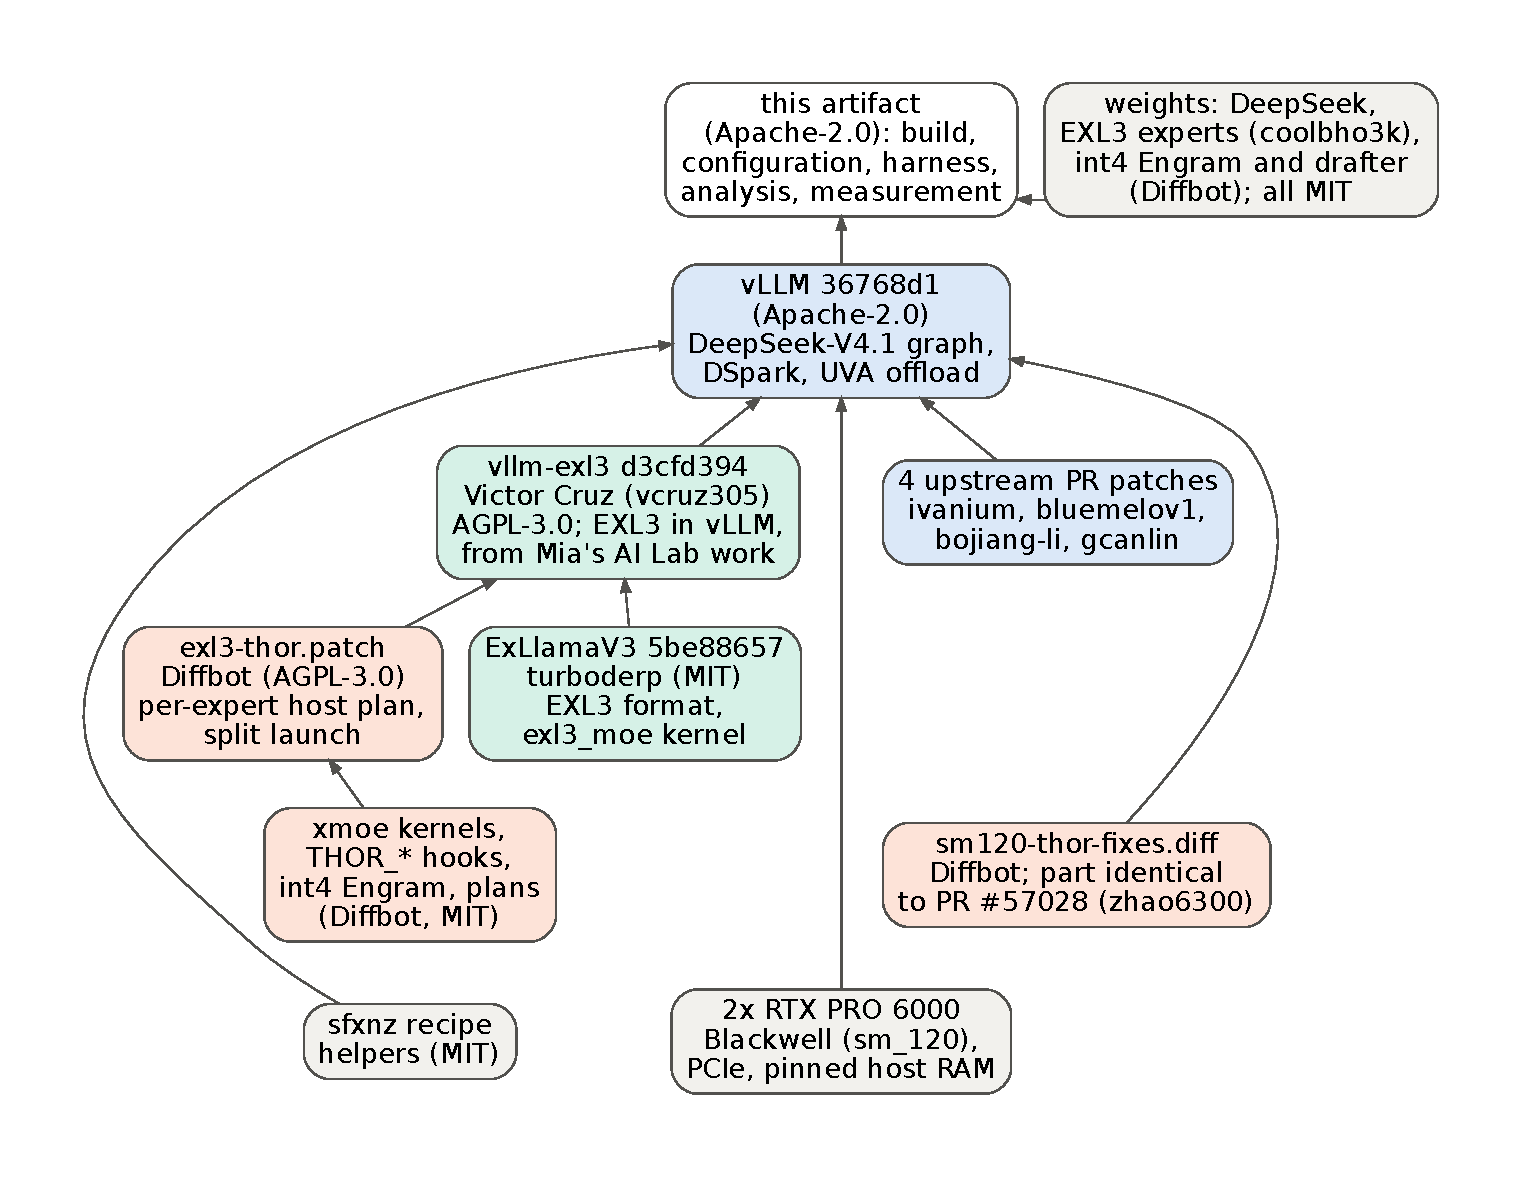
\includegraphics[width=\linewidth]{figures/generated/stack_provenance.pdf}
\caption{Layers of the measured stack and their authors (from \datafile{audit/ATTRIBUTION.md}, rendered from
\datafile{diagrams/stack_provenance.dot}). Orange: Diffbot's recipe. Blue: vLLM and upstream pull requests. Green:
EXL3 format and plugin.}
\label{fig:provenance}
\end{figure}

\paragraph{The people behind each layer.}
DeepSeek released the model's weights under the MIT license. turboderp wrote ExLlamaV3, its EXL3 weight format and the
\texttt{exl3\_moe} kernel that decodes compressed weights inside the matrix product, and coolbho3k quantized the
routed experts to \dv{cfg.exl3_bits} bits in that format. Victor Cruz (vcruz305) wrote vllm-exl3, the plugin that
brings EXL3 routed experts into vLLM, building on earlier work by Mia's AI Lab. That plugin is the foundation of the
whole arrangement. Diffbot's host-expert code is a patch to it, so none of the configurations we measure would run
without it. Diffbot wrote what makes the model fit: a plan file that lists, for every layer, which experts are cold
enough to live in host memory, chosen from routing counts over several traffic profiles, together with the kernels
and the split launch that compute those experts from host memory on a second CUDA stream while the hot experts run in
GPU memory. vLLM provides the serving engine, the DeepSeek-V4.1 graph, the DSpark speculative decoder and the
zero-copy reads of the Engram tables. Four upstream pull requests by ivanium, bluemelov1, bojiang-li and gcanlin, and
the runtime hooks of the sfxnz recipe, fill the remaining gaps. Table~\ref{tab:attribution} lists each feature with
its author and the class of contribution.

\paragraph{Three findings of the audit.}
First, the mechanism underneath the offload was not new inside the stack. Upstream vLLM at the pinned commit already
offers zero-copy weight offload with selection by parameter name, at the granularity of whole tensors, and Victor Cruz
documented an experimental placement of EXL3 expert payloads in pinned host memory two days after that commit and
before Diffbot's publication (\datafile{audit/evidence/vllm_upstream_offload.txt}). What Diffbot added is the
per-expert granularity, the profile-driven choice of which experts go out, and the kernels that make reading them
fast. Second, part of Diffbot's patch for the RTX PRO 6000's architecture (sm\_120) is identical to an open upstream
pull request by another author (zhao6300), which Diffbot's notices credit only in part. Third, our own share is small:
a build without docker, two serving settings (a larger maximum batch, and CUDA graph sizes capped low enough to avoid
a code path that graph capture cannot run), and everything that measures, from the load generator and the samplers to
the harness and the analysis (\datafile{audit/evidence/fat_any_item.txt}).

\begin{table}[t]
\centering\small
\begin{tabular}{p{4.3cm}p{3.4cm}p{3.4cm}l}
\toprule
feature & author & where & class \\
\midrule
DeepSeek-V4.1 graph, DSpark, Engram UVA offload, selective UVA weight offload & vLLM project & vLLM \texttt{36768d1} & implementation \\
EXL3 format and \texttt{exl3\_moe} kernel & turboderp & ExLlamaV3 \texttt{5be88657} & implementation \\
EXL3 support in vLLM & Victor Cruz (vcruz305), from Mia's AI Lab work & vllm-exl3 \texttt{d3cfd394} & implementation \\
EXL3 \dv{cfg.exl3_bits}-bit routed experts & coolbho3k & Hub checkpoint & artifact \\
per-expert host plan, split launch, side-stream SM budget & Diffbot & \texttt{exl3-thor.patch} & algorithmic + implementation \\
plan selection from routing counts & Diffbot & recipe \texttt{plans/} & heuristic \\
xmoe decode and decode-once prefill kernels & Diffbot (from ExLlamaV3) & recipe \texttt{kernels/} & implementation \\
int4 Engram format and lookup, host embedding, FP8 trims & Diffbot & recipe patches and hooks & implementation \\
sm\_120 fixes & Diffbot and zhao6300 (PR \#57028) & \texttt{sm120-thor-fixes.diff} & implementation \\
four upstream PR patches & ivanium, bluemelov1, bojiang-li, gcanlin & recipe \texttt{patches/vllm/} & implementation \\
runtime hooks & sfxnz, edited by Diffbot & \texttt{sitecustomize.py} & integration \\
build without docker, serve settings ($\le$64 sequences, graph sizes $\le$256) & inferencekey (us) & exploratory scripts & configuration \\
load generator, samplers, this harness and analysis & inferencekey (us) & this repository & measurement \\
\bottomrule
\end{tabular}
\caption{Authorship of the features measured in this paper, from the audit (\datafile{audit/ATTRIBUTION.md}, which gives
file:line evidence for every row). ``Class'' follows the audit's classification: algorithmic contribution,
implementation, integration, configuration, or measurement.}
\label{tab:attribution}
\end{table}

When this paper says ``the offload'', it means Diffbot's patch on top of upstream vLLM and Victor Cruz's plugin, run
with the recipe's own settings.

\section{Why the Model Does Not Fit, and How It Is Made To}\label{sec:background}

\paragraph{Why this model.}
On LiveBench~\citep{white2025livebench}, the unquantized model at maximum reasoning effort, as served by DeepSeek,
scores \dv{livebench.deepseek-v4.1-flash-max.All} overall against \dv{livebench.claude-opus-5-5-max-effort.All} for
Claude Opus 5.5 and \dv{livebench.claude-fable-5-1-max-effort.All} for Claude Fable 5.1 at maximum effort. On agentic
coding it is first of the \dv{livebench.n_models} models listed, at
\dv{livebench.deepseek-v4.1-flash-max.Agentic_Coding} against \dv{livebench.agentic.runner_up} for the next
(Figure~\ref{fig:livebench}, Table~\ref{tab:livebench}). The leaderboard data were downloaded on 2026-10-07 and are
stored with hashes in \datafile{data/static/livebench/}~\citep{livebench2026leaderboard}. These are third-party scores
of a different configuration. We serve a \dv{cfg.exl3_bits}-bit pack with thinking disabled, which was not evaluated
on LiveBench, so the scores say why the model is worth serving on modest hardware and are not results of this paper.

\begin{figure}[t]
\centering
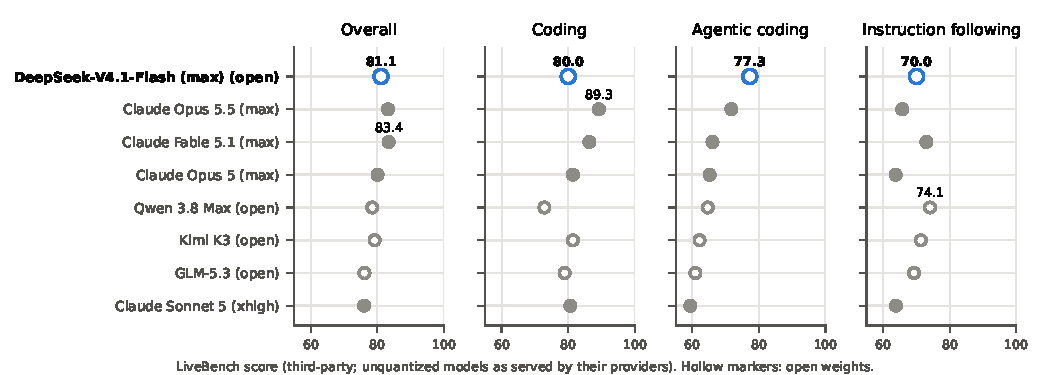
\includegraphics[width=\linewidth]{figures/generated/livebench.pdf}
\caption{Third-party context, not a measurement of this paper: LiveBench scores (question set 2026-06-25, downloaded
2026-10-07) of the unquantized models as served by their providers at the named reasoning effort. DeepSeek-V4.1-Flash
(highlighted) is the maximum-effort, thinking-on configuration. The 3-bit, thinking-off stack studied here was not
evaluated on LiveBench. Hollow markers are open-weight models. Values are labelled for DeepSeek-V4.1-Flash and the best
model of each panel. Source: \datafile{data/static/livebench/}.}
\label{fig:livebench}
\end{figure}

% Generated by hostoffload.analysis.pipeline. Do not edit.
\begin{table}[t]
\centering
\small
\begin{fittable}{tab:livebench}
\begin{tabular}{lrrrr}
\toprule
model & Overall & Coding & Agentic coding & Instruction following \\
\midrule
DeepSeek-V4.1-Flash (max) $^{\circ}$ & 81.1 & 80.0 & 77.3 & 70.0 \\
Claude Opus 5.5 (max) & 83.2 & 89.3 & 71.7 & 65.7 \\
Claude Fable 5.1 (max) & 83.4 & 86.4 & 66.1 & 73.0 \\
Claude Opus 5 (max) & 80.1 & 81.4 & 65.2 & 63.8 \\
Qwen 3.8 Max $^{\circ}$ & 78.5 & 72.9 & 64.6 & 74.1 \\
Kimi K3 $^{\circ}$ & 79.2 & 81.4 & 62.2 & 71.4 \\
GLM-5.3 $^{\circ}$ & 76.1 & 79.0 & 60.9 & 69.3 \\
Claude Sonnet 5 (xhigh) & 76.0 & 80.7 & 59.4 & 63.9 \\
\bottomrule
\end{tabular}
\end{fittable}
\caption{Third-party context: LiveBench scores of the unquantized models as served by their providers at the named reasoning effort (question set 2026-06-25, data downloaded 2026-10-07, \texttt{data/static/livebench/}). $^{\circ}$ open weights. The DeepSeek-V4.1-Flash row is maximum effort with thinking on; the 3-bit stack measured in this paper (thinking off) was not evaluated on LiveBench.}
\label{tab:livebench}
\end{table}


\paragraph{A team of specialists.}
Picture a very large team of specialists, of whom only a few are consulted for any given word. That is a
mixture-of-experts model. Each of DeepSeek-V4.1-Flash's \dv{cfg.num_hidden_layers}
layers~\citep{deepseekai2026v41flash,deepseekai2026v41flashcard} has \dv{cfg.n_routed_experts} routed experts plus
\dv{cfg.n_shared_experts} shared one, and a router sends each token (a piece of a word) to only
\dv{cfg.num_experts_per_tok} of the \dv{cfg.n_routed_experts}. Most specialists are idle at any moment, but all of them
have to be somewhere the GPU can reach, and together they hold most of the model's bytes:
\dv{static.orig.routed_expert_gib}\,GiB of the \dv{static.orig.total_gib}\,GiB checkpoint. The offload rests on that
picture. A specialist who is rarely consulted can wait in a back room, the host's memory, as long as the GPU can still
reach it when the router calls. The rest of this section shows that the back room is necessary on two 96\,GB GPUs and
how the stack uses it.

\paragraph{Making the specialists smaller.}
The first step is compression. EXL3, the format of ExLlamaV3~\citep{turboderp2026exllamav3}, belongs to the
trellis-coded family of QTIP~\citep{tseng2024qtip}. Weights are rotated with Hadamard transforms so that no single
value dominates, then encoded as paths through a trellis with a small codebook, and a GPU kernel decodes them tile by
tile inside the matrix product. The served pack stores the routed experts at \dv{cfg.exl3_bits} bits per
weight~\citep{coolbho3k2026dsv41exl3} and keeps the other weights in DeepSeek's FP8. One routed expert shrinks from
\dv{static.orig.expert_mib}\,MiB in the original checkpoint to \dv{static.expert_mib}\,MiB, and all routed experts
together from \dv{static.orig.routed_expert_gib} to \dv{static.pack.routed_expert_gib}\,GiB.

\paragraph{Compression is not enough.}\label{sec:system}
We accounted every tensor of both checkpoints by class, from their safetensors headers fetched with HTTP range
requests (\dv{static.pack.n_tensors} tensors and \dv{static.pack.total_gib}\,GiB for the pack, with no weights
downloaded), and from placement rules that mirror the documented configuration
(\datafile{src/hostoffload/weights/split.py}, Table~\ref{tab:static-placement}). Even with the large tables and the
embedding in host memory, the pack's GPU-resident weights come to \dv{static.noplan.vram_gib}\,GiB, or
\dv{static.noplan.vram_per_gpu_gib}\,GiB per GPU, against the \dv{expl.gpu_total_gib}\,GiB the driver reports per
card before any KV cache, CUDA graph or activation. That is \dv{expl.noplan_over_per_gpu_gib}\,GiB too much per card.
The original checkpoint is far out of reach, with \dv{static.orig.vram_min_gib}\,GiB outside its Engram tables and
embedding.

% Generated by hostoffload.analysis.pipeline. Do not edit.
\begin{table}[t]
\centering
\small
\begin{fittable}{tab:static-placement}
\begin{tabular}{lrrrrr}
\toprule
tensor class & original & EXL3 pack & VRAM & host & other \\
\midrule
routed experts (40 layers) & 268.95 & 190.48 & 133.34 & 57.14 &  \\
Engram tables & 188.83 & 103.00 & 0.00 & 103.00 &  \\
attention and indexer & 4.80 & 4.80 & 4.80 & 0.00 &  \\
drafter experts & 6.72 & 4.76 & 2.58 & 2.18 &  \\
shared experts & 1.42 & 1.42 & 1.42 & 0.00 &  \\
token embedding & 1.23 & 1.23 & 0.00 & 1.23 &  \\
lm head & 1.23 & 1.23 & 1.23 & 0.00 &  \\
vision tower & 0.90 & 0.90 & 0.00 & 0.00 & not loaded \\
Engram projections & 0.29 & 0.59 & 0.59 & 0.00 &  \\
drafter dense & 0.56 & 0.56 & 0.56 & 0.00 &  \\
routers & 0.15 & 0.15 & 0.15 & 0.00 &  \\
norms, hyper-connections & 0.15 & 0.15 & 0.15 & 0.00 &  \\
\textbf{total} & 475.24 & 309.28 & 144.81 & 163.56 & 0.90 \\
\bottomrule
\end{tabular}
\end{fittable}
\par\smallskip\parbox{0.95\linewidth}{\footnotesize\raggedright Sources: \texttt{data/static/weights/deepseek-ai-2cba9e42/placement.json}, \texttt{data/static/weights/diffbot-a1cf1bd2/placement.json}.}
\caption{Checkpoint bytes by tensor class (GiB, from safetensors headers) for DeepSeek's original checkpoint and the served EXL3 pack, and where the pack's bytes go under the \texttt{gen30} host-expert plan with the documented placement rules (text-only serving). File bytes, not runtime allocations. Static measurement.}
\label{tab:static-placement}
\end{table}


\paragraph{The back room.}
Diffbot's plans close the gap by moving the least-used experts to pinned host memory. All the plans published with the
recipe put \dv{static.gen30.host_target_experts} of the \dv{static.target_experts} target experts on the host
(\dv{static.gen30.host_target_share_pct}\%, between \dv{static.gen30.host_per_layer_min} and
\dv{static.gen30.host_per_layer_max} per layer, Figure~\ref{fig:hostperlayer}). They differ in which experts, chosen
from the routing counts of different traffic. Two other large objects live in the back room in every configuration:
the Engram tables~\citep{cheng2026engram}, two lookup tables indexed by hashed word sequences that give the model
memory by lookup rather than by computation (compressed to int4, from \dv{static.orig.engram_table_gib} to
\dv{static.pack.engram_table_gib}\,GiB), and the token embedding. With the \texttt{gen30} plan the pack's GPU share
drops to \dv{static.gen30.vram_per_gpu_gib}\,GiB per GPU, and \dv{static.gen30.host_gib}\,GiB of file bytes sit on the
host, \dv{static.gen30.host_expert_gib}\,GiB of them experts. Figure~\ref{fig:memarch} shows where everything lives.

The back room is reached without copies. CUDA can register host memory as pinned and map it into the GPU's address
space (unified virtual addressing, or UVA), so that a kernel dereferencing such a pointer reads the data over PCIe, the bus between each GPU and the
computer's main memory, at the moment of use, with no explicit transfer and no cache on the GPU
side~\citep{nvidia2026cudaguide}. This is called zero-copy access. Upstream vLLM already serves the Engram tables this way, and Diffbot's patch does
the same for the cold experts. At each expert layer the patched plugin launches the GPU-resident experts on the main
CUDA stream and the host experts on a second stream limited to a few of the GPU's compute units (SMs), so that the
slow reads over PCIe overlap with the fast work in GPU memory. Because these reads are not copies, a profiler does not
show them as transfers. They appear in the PCIe throughput counters, which our samplers record.

\begin{figure}[t]
\centering
\resizebox{\linewidth}{!}{% Memory architecture of the measured stack. Every number is a \dv value from data/ (static file bytes or the
% exploratory server log). Only the layout is hand-written.
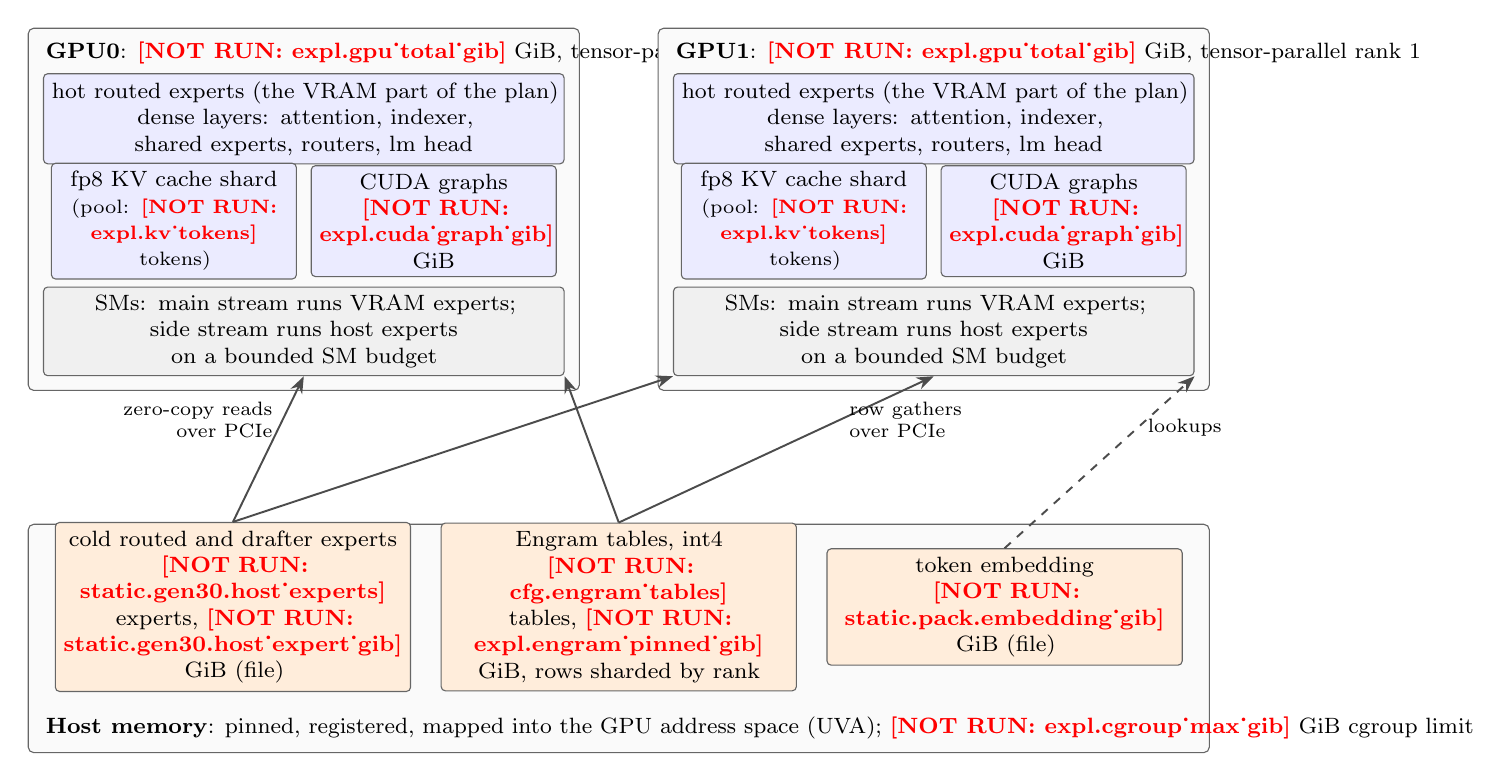
\begin{tikzpicture}[
  font=\footnotesize, >=Stealth,
  box/.style={draw=black!60, rounded corners=1.5pt, align=center, inner sep=3pt, line width=0.4pt},
  vram/.style={box, fill=blue!8},
  host/.style={box, fill=orange!14, text width=4.3cm},
  link/.style={->, line width=0.7pt, draw=black!70}]
  \foreach \g/\x in {0/0, 1/8} {
    \draw[draw=black!60, rounded corners=2pt, fill=black!2] (\x, 0) rectangle (\x+7, 4.6);
    \node[anchor=north west] at (\x+0.1, 4.55) {\textbf{GPU\g}: \dv{expl.gpu_total_gib} GiB, tensor-parallel rank \g};
    \node[vram, text width=6.4cm] (hot\g) at (\x+3.5, 3.45) {hot routed experts (the VRAM part of the plan)\\
      dense layers: attention, indexer, shared experts, routers, lm head};
    \node[vram, text width=2.9cm] (kv\g) at (\x+1.85, 2.15) {fp8 KV cache shard\\ \scriptsize(pool: \dv{expl.kv_tokens} tokens)};
    \node[vram, text width=2.9cm] (cg\g) at (\x+5.15, 2.15) {CUDA graphs\\ \dv{expl.cuda_graph_gib} GiB};
    \node[box, fill=black!6, text width=6.4cm] (sm\g) at (\x+3.5, 0.75) {SMs: main stream runs VRAM experts;\\
      side stream runs host experts on a bounded SM budget};
  }
  \draw[draw=black!60, rounded corners=2pt, fill=black!2] (0, -4.6) rectangle (15, -1.7);
  \node[anchor=south west] at (0.1, -4.55) {\textbf{Host memory}: pinned, registered, mapped into the GPU address
    space (UVA); \dv{expl.cgroup_max_gib} GiB cgroup limit};
  \node[host] (cold) at (2.6, -2.75) {cold routed and drafter experts\\ \dv{static.gen30.host_experts} experts,
    \dv{static.gen30.host_expert_gib} GiB (file)};
  \node[host] (engram) at (7.5, -2.75) {Engram tables, int4\\ \dv{cfg.engram_tables} tables,
    \dv{expl.engram_pinned_gib} GiB, rows sharded by rank};
  \node[host] (emb) at (12.4, -2.75) {token embedding\\ \dv{static.pack.embedding_gib} GiB (file)};
  \draw[link] (cold.north) -- node[pos=0.7, left, align=right, font=\scriptsize] {zero-copy reads\\ over PCIe} (sm0.south);
  \draw[link] (cold.north) -- (sm1.south west);
  \draw[link] (engram.north) -- node[pos=0.7, right, font=\scriptsize, align=left] {row gathers\\ over PCIe} (sm1.south);
  \draw[link] (engram.north) -- (sm0.south east);
  \draw[link, dashed] (emb.north) -- node[pos=0.7, right, font=\scriptsize] {lookups} (sm1.south east);
\end{tikzpicture}
}
\caption{Memory architecture of the measured stack (two GPUs, tensor parallel). Blue: GPU memory (VRAM). Orange:
pinned host memory that GPU kernels read over PCIe by zero-copy access (UVA). Sizes are checkpoint bytes from the safetensors headers
(\datafile{data/static/weights/diffbot-a1cf1bd2/placement.json}) or values the server logged at load in the exploratory
run (KV tokens, CUDA graph memory, Engram tables), all printed from data files.}
\label{fig:memarch}
\end{figure}

\begin{figure}[t]
\centering
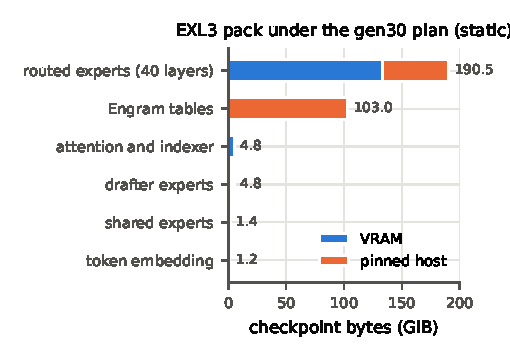
\includegraphics[width=0.49\linewidth]{figures/generated/static_placement.pdf}\hfill
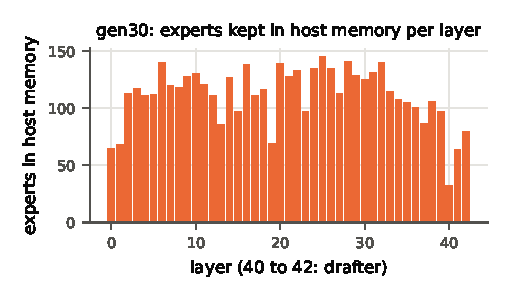
\includegraphics[width=0.49\linewidth]{figures/generated/static_host_per_layer.pdf}
\caption{Static measurement. Left: checkpoint bytes per tensor class in GPU memory and in pinned host memory under the
\texttt{gen30} plan. Right: experts the plan keeps in host memory, per layer (layers 40 to 42 are the drafter).
Source: \datafile{data/static/weights/diffbot-a1cf1bd2/placement.json}.}
\label{fig:hostperlayer}
\end{figure}

\paragraph{Checking the accounting against the server.}
Placement rules are a model, so we checked them where the server reports what it did. The Engram bytes the server
pinned in the exploratory run (\dv{expl.engram_pinned_gib}\,GiB, in four shards of
\dv{expl.engram_per_table_rank_gib}\,GiB) equal the file bytes. The per-layer counts of host experts it logged equal
those of one published plan on every layer, which identifies the plan each exploratory run used
(Section~\ref{sec:results-exploratory}). File bytes are not runtime bytes, though. vLLM reported
\dv{expl.model_loading_gib}\,GiB of weights per GPU, \dv{expl.runtime_minus_file_gib}\,GiB more than the plan's file
bytes in GPU memory, presumably from repacked and duplicated layouts that we did not attribute allocation by
allocation. The exploratory boot also left \dv{expl.headroom_mib}\,MiB of GPU memory unused per card at its peak.
Spending all of it on experts would bring \dv{expl.min_share.movable_experts} of them back, so with this KV budget and
these graph sizes at least \dv{expl.min_share.pct}\% of the target experts must stay on the host. That is an estimate
from one boot, and no run searched for the smallest share that boots.

\paragraph{The boots.}
Experiment E2 tested the accounting on the GPUs (Table~\ref{tab:ctl-E2}). The EXL3 plugin with every expert in GPU
memory and the offload build with an empty plan both stopped while loading, with the server's own out-of-memory
errors. The same offload build with the \texttt{gen30} plan booted and served all the measurements of the next
sections. The byte accounting (E0) and the boots (E2) are specified in Section~\ref{sec:method}, and the pods they ran
on in Section~\ref{sec:setup}.

% Generated by hostoffload.analysis.pipeline. Do not edit.
\begin{table}[t]
\centering
\small
\begin{fittable}{tab:ctl-E2}
\begin{tabular}{lllp{6cm}}
\toprule
configuration & status & failure & first error line \\
\midrule
exl3-min-allvram & boot\_failed & gpu\_oom & \texttt{(Worker\_TP1 pid=11812) ERROR 10-06 20:04:41 [multiproc\_executor.py:948] torch.OutOfMemoryE} \\
exl3-offload-noplan & boot\_failed & gpu\_oom & \texttt{(Worker\_TP1 pid=15785) ERROR 10-06 20:08:11 [multiproc\_executor.py:948] torch.OutOfMemoryE} \\
\bottomrule
\end{tabular}
\end{fittable}
\caption{Controlled: feasibility boots on 2x RTX PRO 6000 (E2). Status and the first matching error line of the server log (\texttt{hostoffload.analysis.failures}).}
\label{tab:ctl-E2}
\end{table}


\section{How Fast the Offloaded Stack Runs}\label{sec:results}\label{sec:results-controlled}

This section measures the speed of the offloaded stack: how long users wait, how fast replies are written, and how
both change with load, prompt length, the share of experts on the host and the host itself. It cannot say how much
of any slowdown the offload causes, because the reference with everything in GPU memory (E9) did not run. Only the two
host shares of E3 isolate part of that cost (Section~\ref{sec:limits}).

\paragraph{Reading and writing.}
One distinction makes the rest of the section easy to follow. Serving a request has two phases. In the first the model
\emph{reads} the prompt. It processes every prompt token in one pass, which is limited by compute and grows with the
prompt's length. In the second it \emph{writes} the reply one token at a time, and each step must fetch the weights of
the experts the router picks for that token, which is limited by memory traffic, including the reads from the back
room. vLLM~\citep{kwon2023vllm} keeps the KV cache in pages, batches requests continuously and splits long prompts into
chunks that share steps with ongoing replies~\citep{agrawal2024sarathi}. It also caches prompt prefixes, so a request
that shares a prefix with an earlier one skips reading it~\citep{zheng2024sglang,vllm2026prefixcaching}. Two numbers
follow from the two phases. The \emph{time to first token} (TTFT) is how long a user waits before anything appears,
which is mostly reading. The \emph{time per output token} (TPOT) is the pace of writing, and its inverse, the rate per
stream in tokens/s, is what a user perceives as speed. We report medians and tails: a TTFT p95 of 2\,s means that 95\%
of requests waited less than two seconds, and p5 is the slow end of a rate.

The measurements come from three sessions on rented pods with two RTX PRO 6000 GPUs each, on three different hosts
(Table~\ref{tab:pod-hardware}). Each experiment ran on a single boot, so intervals cover repetitions inside a boot and
never variation between boots. All runs used code prompts, DSpark speculative decoding and Diffbot's \texttt{gen30}
plan unless stated. Section~\ref{sec:method} gives the protocol.

\paragraph{One user, then many (E8).}
Start with a single user sending independent 4K-token code prompts. The model writes at a median of
\dv{ctl.E8.stream.A.N1.p50} tokens/s per stream (p5 \dv{ctl.E8.stream.A.N1.p5}, p95 \dv{ctl.E8.stream.A.N1.p95}).
Now add users. At eight, each stream gets a median of \dv{ctl.E8.stream.A.N8.p50} tokens/s, and at 64 only
\dv{ctl.E8.stream.A.N64.p50}. The server as a whole does more work as users arrive, but each user gets a smaller share
of it. With a cached 16K-token prefix, which removes most of the reading, the trade is clearer. The total output grows
from \dv{ctl.E8.main.B-prefix-16k.closed:1.agg_mean} tokens/s with one user to
\dv{ctl.E8.main.B-prefix-16k.closed:32.agg_mean} at 32 and \dv{ctl.E8.main.B-prefix-16k.closed:64.agg_mean} at 64,
while the rate of each stream falls from \dv{ctl.E8.stream.B.N1.p50} to \dv{ctl.E8.stream.B.N32.p50} and
\dv{ctl.E8.stream.B.N64.p50}, and TTFT p95 stays at or below \dv{ctl.E8.main.B-prefix-16k.closed:64.ttft_p95}\,s at
every level. Figure~\ref{fig:ctl-E8} shows both sides of the trade, and Tables~\ref{tab:ctl-E8}
and~\ref{tab:ctl-E8-thr} give every level.

\begin{figure}[t]
\centering
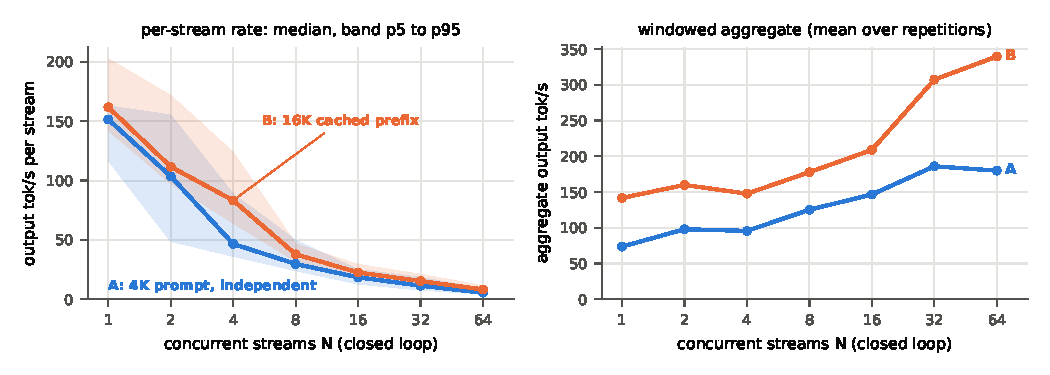
\includegraphics[width=\linewidth]{figures/generated/controlled_E8}
\caption{Controlled E8 sweep (pod 1, \texttt{gen30} plan). Left: output rate per stream against the number of
concurrent users $N$, median with a p5 to p95 band over the requests of each level (warm requests and errors excluded,
repetitions pooled). Right: windowed aggregate output rate, mean over repetitions (two in B, and in A two only at
$N=1$, where the mean includes a slow first repetition). A: independent 4K-token code prompts. B: 16K-token cached
prefix.}
\label{fig:ctl-E8}
\end{figure}

When every user brings a new prompt, reading competes with writing and the total stops growing earlier, at
\dv{ctl.E8.main.A-code-4k.closed:8.agg_mean} tokens/s with eight users, \dv{ctl.E8.main.A-code-4k.closed:32.agg_mean}
with 32 and \dv{ctl.E8.main.A-code-4k.closed:64.agg_mean} with 64, while TTFT p95 rises to
\dv{ctl.E8.main.A-code-4k.closed:64.ttft_p95}\,s. Reading alone, one prompt at a time, takes
\dv{ctl.E8.probes.prefill-4096.closed:1.ttft_p50}, \dv{ctl.E8.probes.prefill-16384.closed:1.ttft_p50} and
\dv{ctl.E8.probes.prefill-65536.closed:1.ttft_p50}\,s for 4K, 16K and 64K tokens. Two caveats apply to this sweep. The
cached-prefix scenario has two repetitions per level, but the unique-prompt scenario has two only for one user. In its
second repetition a single client-side disconnect among eight requests tripped the pre-registered stop rule and ended
the sweep, a rule we have since made less sensitive. That one-user level also pools a slow first repetition (TTFT p95
\dv{ctl.E8.main.A-code-4k.closed:1.ttft_p95}\,s), so its aggregate is not a steady-state rate.

% Generated by hostoffload.analysis.pipeline. Do not edit.
\begin{table}[t]
\centering
\small
\begin{fittable}{tab:ctl-E8}
\begin{tabular}{llrrrrrrrr}
\toprule
scenario & load & $n$ & TTFT p50 & p95 & p99 & TPOT p50 & p95 & E2E p50 & p99 \\
\midrule
\addlinespace\multicolumn{10}{l}{\textit{main}, pod 1} \\
A-code-4k & closed:1 & 16 & 0.65 & 9.44 & 25.81 & 6.6 & 9.6 & 2.3 & 29.4 \\
A-code-4k & closed:2 & 8 & 0.68 & 1.31 & 1.31 & 9.8 & 20.8 & 3.5 & 6.4 \\
A-code-4k & closed:4 & 8 & 0.65 & 1.28 & 1.30 & 22.1 & 27.7 & 6.3 & 8.4 \\
A-code-4k & closed:8 & 16 & 1.13 & 2.26 & 2.26 & 33.6 & 41.5 & 9.4 & 12.6 \\
A-code-4k & closed:16 & 32 & 2.65 & 5.40 & 5.47 & 54.2 & 78.1 & 17.2 & 25.0 \\
A-code-4k & closed:32 & 64 & 3.57 & 10.15 & 10.38 & 87.5 & 130.0 & 26.5 & 39.9 \\
A-code-4k & closed:64 & 128 & 4.77 & 27.29 & 28.85 & 182.2 & 235.2 & 53.2 & 83.4 \\
B-prefix-16k & closed:1 & 16 & 0.30 & 0.31 & 0.32 & 6.2 & 7.0 & 1.9 & 2.2 \\
B-prefix-16k & closed:2 & 16 & 0.42 & 0.45 & 0.46 & 9.0 & 10.3 & 2.6 & 3.1 \\
B-prefix-16k & closed:4 & 16 & 0.44 & 0.58 & 0.68 & 12.0 & 15.6 & 3.5 & 4.7 \\
B-prefix-16k & closed:8 & 32 & 0.52 & 0.82 & 0.89 & 26.4 & 31.4 & 7.3 & 8.9 \\
B-prefix-16k & closed:16 & 64 & 0.78 & 1.07 & 1.16 & 44.3 & 55.9 & 12.1 & 16.3 \\
B-prefix-16k & closed:32 & 128 & 1.19 & 1.59 & 1.66 & 65.3 & 87.7 & 17.9 & 24.9 \\
B-prefix-16k & closed:64 & 256 & 1.67 & 2.03 & 2.18 & 121.1 & 153.0 & 32.3 & 44.1 \\
\addlinespace\multicolumn{10}{l}{\textit{probes}, pod 1} \\
decode & closed:1 & 4 & 0.19 & 0.21 & 0.21 & 6.7 & 7.9 & 3.6 & 4.3 \\
decode & closed:8 & 8 & 0.85 & 0.85 & 0.85 & 21.2 & 22.6 & 11.7 & 12.3 \\
decode & closed:32 & 32 & 15.15 & 15.32 & 15.32 & 59.5 & 66.2 & 45.3 & 49.0 \\
prefill-4096 & closed:1 & 3 & 0.63 & 0.66 & 0.66 & 0.0 & 0.0 & 0.6 & 0.7 \\
prefill-16384 & closed:1 & 3 & 1.56 & 1.60 & 1.60 & 0.0 & 0.0 & 1.6 & 1.6 \\
prefill-65536 & closed:1 & 3 & 6.19 & 6.39 & 6.41 & 0.0 & 0.0 & 6.2 & 6.4 \\
\bottomrule
\end{tabular}
\end{fittable}
\caption{Controlled: Main benchmark of the measured stack as run (gen30 plan; scenarios A and B at N = 1 to 64, two repetitions in B and in A only at N = 1; prefill and decode probes, one repetition). Part 1 of 2, per-request latency: time to first token (TTFT, s), time per output token (TPOT, ms) and end-to-end time (E2E, s), with requests pooled over repetitions. Rows are grouped by variant and pod session (Table~\ref{tab:pod-hardware}). Throughput and SLOs of the same load points: Table~\ref{tab:ctl-E8-thr}.}
\label{tab:ctl-E8}
\end{table}
\begin{table}[t]
\centering
\small
\begin{fittable}{tab:ctl-E8-thr}
\begin{tabular}{llrrrrl}
\toprule
scenario & load & R & $n$ & aggregate tok/s & CV\% & SLO \\
\midrule
\addlinespace\multicolumn{7}{l}{\textit{main}, pod 1} \\
A-code-4k & closed:1 & 2 & 16 & 73.6 & 68.9 & - \\
A-code-4k & closed:2 & 1 & 8 & 97.9 & - & i,r,l \\
A-code-4k & closed:4 & 1 & 8 & 95.6 & - & i,r,l \\
A-code-4k & closed:8 & 1 & 16 & 125.2 & - & r,l \\
A-code-4k & closed:16 & 1 & 32 & 146.5 & - & r \\
A-code-4k & closed:32 & 1 & 64 & 186.0 & - & - \\
A-code-4k & closed:64 & 1 & 128 & 179.9 & - & - \\
B-prefix-16k & closed:1 & 2 & 16 & 141.7 & 5.2 & i,r,l \\
B-prefix-16k & closed:2 & 2 & 16 & 159.9 & 0.8 & i,r,l \\
B-prefix-16k & closed:4 & 2 & 16 & 147.7 & 4.6 & i,r,l \\
B-prefix-16k & closed:8 & 2 & 32 & 177.7 & 5.7 & i,r,l \\
B-prefix-16k & closed:16 & 2 & 64 & 208.9 & 7.2 & r,l \\
B-prefix-16k & closed:32 & 2 & 128 & 307.2 & 4.3 & r \\
B-prefix-16k & closed:64 & 2 & 256 & 339.5 & 7.5 & - \\
\addlinespace\multicolumn{7}{l}{\textit{probes}, pod 1} \\
decode & closed:1 & 1 & 4 & 133.2 & - & i,r,l \\
decode & closed:8 & 1 & 8 & 333.3 & - & i,r,l \\
decode & closed:32 & 1 & 32 & 334.5 & - & - \\
prefill-4096 & closed:1 & 1 & 3 & 1.6 & - & - \\
prefill-16384 & closed:1 & 1 & 3 & 0.6 & - & - \\
prefill-65536 & closed:1 & 1 & 3 & 0.2 & - & - \\
\bottomrule
\end{tabular}
\end{fittable}
\caption{Controlled: Main benchmark of the measured stack as run (gen30 plan; scenarios A and B at N = 1 to 64, two repetitions in B and in A only at N = 1; prefill and decode probes, one repetition). Part 2 of 2, throughput and objectives. R: repetitions at that point; aggregate: mean over repetitions of the windowed output rate (tokens/s), CV its coefficient of variation across repetitions (- for a single repetition); SLO: initials of the pre-registered SLOs met in every repetition. Latency of the same load points: Table~\ref{tab:ctl-E8}.}
\label{tab:ctl-E8-thr}
\end{table}


The same trade sets the cost of a token. At \dv{price.2xpro6000.usd_h}\,USD per pod-hour, with the whole hour charged
to output tokens (an upper bound for output that says nothing about input), one million output tokens cost
\dv{ctl.E8.main.B-prefix-16k.closed:1.usd_per_m_out}\,USD with one user on the cached prefix and
\dv{ctl.E8.main.B-prefix-16k.closed:64.usd_per_m_out}\,USD with 64, and \dv{ctl.E8.main.A-code-4k.closed:8.usd_per_m_out}
and \dv{ctl.E8.main.A-code-4k.closed:32.usd_per_m_out}\,USD at eight and 32 users with unique prompts, so the
cheapest tokens are those written when each stream is slowest. We registered three service-level objectives before
the controlled runs (Section~\ref{sec:method}). With the cached prefix the interactive one (TTFT p95 up to 2\,s and
TPOT p95 up to 50\,ms) holds in every repetition up to eight users and the relaxed one up to 32. With unique prompts
the interactive objective holds from two to four users and the relaxed one from two to 16, and the one-user level
misses both because of its slow first repetition (SLO column of Table~\ref{tab:ctl-E8-thr}). For coding agents the useful unit is the number of streams that stay fast, which is the
subject of Section~\ref{sec:agent}.\label{sec:cost}

\paragraph{Long prompts cost reading (E12).}
Coding agents work with long contexts, so we pushed the prompt to the context limit of
\dv{ctl.kv.max_len} tokens on the second pod. Reading grows as expected. A fresh prompt of 128K tokens waits
\dv{ctl.E12.long.prefill-long-131072.closed:1.ttft_p50}\,s for its first token, and one of 260,000 tokens
\dv{ctl.E12.long.prefill-long-260000.closed:1.ttft_p50}\,s. Writing by a single request hardly notices the length. It
takes \dv{ctl.E12.long.decode-128k.closed:1.tpot_p50_ms}\,ms per token after a 128K-token prompt and
\dv{ctl.E12.long.decode-256k.closed:1.tpot_p50_ms}\,ms after a 256K-token one, against
\dv{ctl.E3.gen30-session2.A-code-4k.closed:1.tpot_p50_ms}\,ms after a 4K-token prompt on the same pod. That changes
when several long requests write at once, at \dv{ctl.E12.long.decode-128k.closed:4.tpot_p50_ms}\,ms per token with
four 128K requests and \dv{ctl.E12.long.decode-256k.closed:2.tpot_p50_ms}\,ms with two of 256K.
Figure~\ref{fig:read-write} puts the two phases side by side: reading climbs with the length of the prompt, and
writing stays flat.

\begin{figure}[t]
\centering
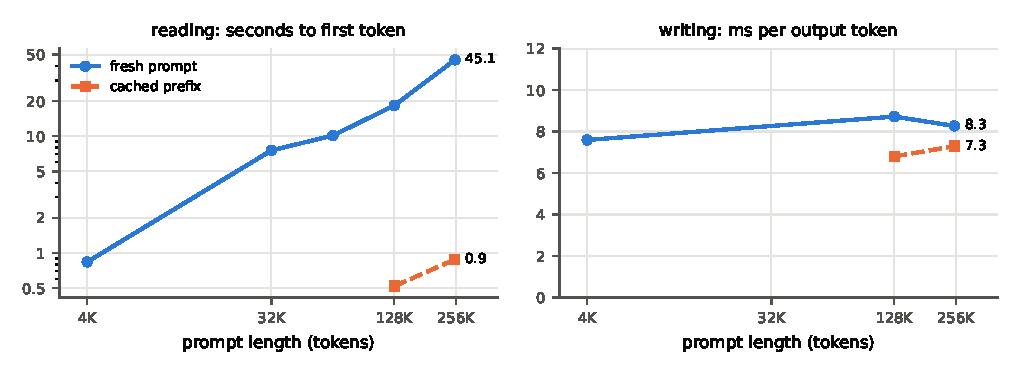
\includegraphics[width=\linewidth]{figures/generated/read_write_length.pdf}
\caption{Reading against writing for one request on pod~2 (one repetition, median of 2 to 8 requests per point).
Left: time to first token against prompt length, for fresh prompts and for prompts behind a cached prefix (log
scales). Right: time per output token against prompt length. The 4K point is the E3 \texttt{gen30} run on the same
pod, and the other points are E12. Values from Tables~\ref{tab:ctl-E12} and~\ref{tab:ctl-E3}, lengths from
\datafile{experiments/workloads/long_context.yaml}.}
\label{fig:read-write}
\end{figure}

When the long context is shared and cached, as for agents working on one large codebase, the reading is paid once.
With a 128K-token cached prefix, TTFT p95 is \dv{ctl.E12.long.B-prefix-128k.closed:8.ttft_p95}\,s at eight users, and
with 256K tokens it is \dv{ctl.E12.long.B-prefix-256k.closed:4.ttft_p95}\,s at four users with
\dv{ctl.E12.long.B-prefix-256k.closed:4.tpot_p50_ms}\,ms per token. A long context therefore stays interactive once it
has been read, and the expensive case is many users with different long prompts, where reading sets the limit. vLLM's
estimate of how many full-length requests fit in the KV cache (\dv{ctl.kv.max_concurrency}) is why E12 ran distinct
long prompts only up to four at 128K and two at 256K, and Section~\ref{sec:agent} shows that the estimate is
conservative. Each point is one repetition, on the second pod, which was slower than the first, and without a quality
check at these lengths (Tables~\ref{tab:ctl-E12} and~\ref{tab:ctl-E12-thr}).

% Generated by hostoffload.analysis.pipeline. Do not edit.
\begin{table}[t]
\centering
\small
\begin{fittable}{tab:ctl-E12}
\begin{tabular}{llrrrrrrrr}
\toprule
scenario & load & $n$ & TTFT p50 & p95 & p99 & TPOT p50 & p95 & E2E p50 & p99 \\
\midrule
\addlinespace\multicolumn{10}{l}{\textit{long}, pod 2} \\
B-prefix-128k & closed:1 & 4 & 0.52 & 0.57 & 0.57 & 6.8 & 7.2 & 2.3 & 2.3 \\
B-prefix-128k & closed:2 & 4 & 0.54 & 0.68 & 0.70 & 8.7 & 11.1 & 2.8 & 3.4 \\
B-prefix-128k & closed:4 & 8 & 0.66 & 1.19 & 1.33 & 13.2 & 19.2 & 4.0 & 6.1 \\
B-prefix-128k & closed:8 & 16 & 0.79 & 1.18 & 1.24 & 38.3 & 46.7 & 10.5 & 12.7 \\
B-prefix-256k & closed:1 & 4 & 0.88 & 0.89 & 0.89 & 7.3 & 7.5 & 2.7 & 2.8 \\
B-prefix-256k & closed:2 & 4 & 0.93 & 0.94 & 0.94 & 9.9 & 10.8 & 3.5 & 3.7 \\
B-prefix-256k & closed:4 & 8 & 1.26 & 1.66 & 1.70 & 16.6 & 19.6 & 5.4 & 6.1 \\
decode-128k & closed:1 & 2 & 22.45 & 25.13 & 25.36 & 8.7 & 10.4 & 26.9 & 28.9 \\
decode-128k & closed:2 & 2 & 27.10 & 34.05 & 34.67 & 29.1 & 43.1 & 42.0 & 42.2 \\
decode-128k & closed:4 & 4 & 48.20 & 71.72 & 73.77 & 68.4 & 118.4 & 83.7 & 84.2 \\
decode-256k & closed:1 & 2 & 44.75 & 47.79 & 48.06 & 8.3 & 9.3 & 49.0 & 52.9 \\
decode-256k & closed:2 & 2 & 58.74 & 75.79 & 77.30 & 48.2 & 81.8 & 83.3 & 83.5 \\
prefill-long-32768 & closed:1 & 3 & 7.57 & 10.75 & 11.04 & 0.0 & 0.0 & 7.6 & 11.0 \\
prefill-long-65536 & closed:1 & 3 & 10.14 & 14.91 & 15.34 & 0.0 & 0.0 & 10.1 & 15.3 \\
prefill-long-131072 & closed:1 & 3 & 18.33 & 18.46 & 18.48 & 0.0 & 0.0 & 18.3 & 18.5 \\
prefill-long-260000 & closed:1 & 3 & 45.07 & 58.68 & 59.89 & 0.0 & 0.0 & 45.1 & 59.9 \\
\bottomrule
\end{tabular}
\end{fittable}
\caption{Controlled: Long context at 128K and 256K tokens as run (pod 2; prefill, decode and cached shared prefix, one repetition). Part 1 of 2, per-request latency: time to first token (TTFT, s), time per output token (TPOT, ms) and end-to-end time (E2E, s), with requests pooled over repetitions. Rows are grouped by variant and pod session (Table~\ref{tab:pod-hardware}). Throughput and SLOs of the same load points: Table~\ref{tab:ctl-E12-thr}.}
\label{tab:ctl-E12}
\end{table}
\begin{table}[t]
\centering
\small
\begin{fittable}{tab:ctl-E12-thr}
\begin{tabular}{llrrrrl}
\toprule
scenario & load & R & $n$ & aggregate tok/s & CV\% & SLO \\
\midrule
\addlinespace\multicolumn{7}{l}{\textit{long}, pod 2} \\
B-prefix-128k & closed:1 & 1 & 4 & 111.0 & - & i,r,l \\
B-prefix-128k & closed:2 & 1 & 4 & 90.9 & - & i,r,l \\
B-prefix-128k & closed:4 & 1 & 8 & 115.3 & - & i,r,l \\
B-prefix-128k & closed:8 & 1 & 16 & 126.8 & - & i,r,l \\
B-prefix-256k & closed:1 & 1 & 4 & 92.5 & - & i,r,l \\
B-prefix-256k & closed:2 & 1 & 4 & 91.8 & - & i,r,l \\
B-prefix-256k & closed:4 & 1 & 8 & 177.9 & - & i,r,l \\
decode-128k & closed:1 & 1 & 2 & 20.6 & - & - \\
decode-128k & closed:2 & 1 & 2 & 24.3 & - & - \\
decode-128k & closed:4 & 1 & 4 & 24.3 & - & - \\
decode-256k & closed:1 & 1 & 2 & 11.4 & - & - \\
decode-256k & closed:2 & 1 & 2 & 12.3 & - & - \\
prefill-long-32768 & closed:1 & 1 & 3 & 0.1 & - & - \\
prefill-long-65536 & closed:1 & 1 & 3 & 0.1 & - & - \\
prefill-long-131072 & closed:1 & 1 & 3 & 0.1 & - & - \\
prefill-long-260000 & closed:1 & 1 & 3 & 0.0 & - & - \\
\bottomrule
\end{tabular}
\end{fittable}
\caption{Controlled: Long context at 128K and 256K tokens as run (pod 2; prefill, decode and cached shared prefix, one repetition). Part 2 of 2, throughput and objectives. R: repetitions at that point; aggregate: mean over repetitions of the windowed output rate (tokens/s), CV its coefficient of variation across repetitions (- for a single repetition); SLO: initials of the pre-registered SLOs met in every repetition. Latency of the same load points: Table~\ref{tab:ctl-E12}.}
\label{tab:ctl-E12-thr}
\end{table}


\paragraph{The size of the back room (E3).}
Putting more experts in the back room costs speed. Moving from the \texttt{gen30} plan to the union of its cold set
and that of the recipe's \texttt{agent30} plan lowers the total output with unique code prompts from
\dv{ctl.E3.gen30.A-code-4k.closed:1.agg_mean} to \dv{ctl.E3.union-gen30-agent30.A-code-4k.closed:1.agg_mean}
tokens/s with one user, from \dv{ctl.E3.gen30.A-code-4k.closed:8.agg_mean} to
\dv{ctl.E3.union-gen30-agent30.A-code-4k.closed:8.agg_mean} with eight and from
\dv{ctl.E3.gen30.A-code-4k.closed:32.agg_mean} to \dv{ctl.E3.union-gen30-agent30.A-code-4k.closed:32.agg_mean} with 32
(Table~\ref{tab:ctl-E3-thr}, one repetition per point, two boots). The decode scenario of the larger share is missing,
because the load generator stopped on a client-side disconnect while the server kept serving.

We also wanted to compare Diffbot's per-expert machinery with the zero-copy offload that upstream vLLM already ships,
at the same host bytes. We could not compare speed, because upstream's offload does not serve this model on these
pins. With the KV block size of 64 that the measured stack uses, it fails at initialization, since the FlashInfer
sparse-attention backend for DeepSeek-V4.1 accepts only blocks of 128. With 128 the server boots, and the engine dies
on the first request, because DeepGEMM's attention kernel asserts a block of 32 or 64
(\datafile{data/controlled/E3-host-share/uva-equal-gen30/} and \datafile{data/controlled/E3-host-share/uva-equal-gen30-bs128/}). Two kernels on the
same attention path accept different block sizes, and with the recipe's runtime hooks (sfxnz's, edited by Diffbot)
the stack serves with blocks of 64. On this hardware and these pins the hooks are needed to serve at all, so whether
the per-expert split is also faster than upstream's offload remains open.

% Generated by hostoffload.analysis.pipeline. Do not edit.
\begin{table}[t]
\centering
\small
\begin{fittable}{tab:ctl-E3}
\begin{tabular}{llrrrrrrrr}
\toprule
scenario & load & $n$ & TTFT p50 & p95 & p99 & TPOT p50 & p95 & E2E p50 & p99 \\
\midrule
\addlinespace\multicolumn{10}{l}{\textit{gen30}, pod 1} \\
A-code-4k & closed:1 & 8 & 0.64 & 0.66 & 0.66 & 6.5 & 7.0 & 2.3 & 2.4 \\
A-code-4k & closed:8 & 16 & 1.05 & 1.70 & 1.72 & 31.3 & 35.4 & 8.8 & 10.9 \\
A-code-4k & closed:32 & 64 & 3.38 & 9.05 & 9.56 & 86.6 & 111.1 & 26.0 & 36.9 \\
decode & closed:1 & 4 & 0.21 & 0.21 & 0.21 & 6.0 & 6.4 & 3.3 & 3.5 \\
decode & closed:8 & 8 & 0.83 & 0.84 & 0.84 & 21.3 & 22.1 & 11.6 & 12.2 \\
decode & closed:32 & 32 & 1.33 & 1.33 & 1.46 & 60.2 & 67.5 & 32.1 & 36.4 \\
\addlinespace\multicolumn{10}{l}{\textit{gen30-session2}, pod 2} \\
A-code-4k & closed:1 & 8 & 0.84 & 10.89 & 15.21 & 7.6 & 7.9 & 2.8 & 17.1 \\
A-code-4k & closed:8 & 16 & 1.65 & 2.81 & 2.87 & 43.3 & 55.2 & 13.2 & 16.0 \\
A-code-4k & closed:32 & 64 & 4.88 & 17.75 & 18.41 & 130.9 & 180.1 & 38.5 & 61.9 \\
decode & closed:1 & 4 & 0.22 & 0.24 & 0.24 & 7.4 & 9.4 & 4.0 & 5.1 \\
decode & closed:8 & 8 & 0.94 & 0.94 & 0.94 & 29.4 & 30.4 & 15.7 & 16.6 \\
decode & closed:32 & 32 & 12.33 & 12.33 & 12.50 & 77.2 & 90.3 & 51.5 & 58.6 \\
\addlinespace\multicolumn{10}{l}{\textit{union-gen30-agent30}, pod 1} \\
A-code-4k & closed:1 & 8 & 0.88 & 1.76 & 2.12 & 8.7 & 9.7 & 3.2 & 4.3 \\
A-code-4k & closed:8 & 16 & 1.92 & 2.77 & 2.77 & 42.0 & 54.8 & 12.6 & 16.5 \\
A-code-4k & closed:32 & 64 & 4.51 & 13.03 & 13.65 & 121.2 & 165.2 & 36.3 & 53.7 \\
\bottomrule
\end{tabular}
\end{fittable}
\caption{Controlled: Host share as run (rung (c) of the ablation ladder): the gen30 plan against the union of the gen30 and agent30 cold sets on pod 1, and the gen30 subset repeated on pod 2 (variant gen30-session2), one repetition per point. Part 1 of 2, per-request latency: time to first token (TTFT, s), time per output token (TPOT, ms) and end-to-end time (E2E, s), with requests pooled over repetitions. Rows are grouped by variant and pod session (Table~\ref{tab:pod-hardware}). Throughput and SLOs of the same load points: Table~\ref{tab:ctl-E3-thr}.}
\label{tab:ctl-E3}
\end{table}
\begin{table}[t]
\centering
\small
\begin{fittable}{tab:ctl-E3-thr}
\begin{tabular}{llrrrrl}
\toprule
scenario & load & R & $n$ & aggregate tok/s & CV\% & SLO \\
\midrule
\addlinespace\multicolumn{7}{l}{\textit{gen30}, pod 1} \\
A-code-4k & closed:1 & 1 & 8 & 112.1 & - & i,r,l \\
A-code-4k & closed:8 & 1 & 16 & 146.6 & - & i,r,l \\
A-code-4k & closed:32 & 1 & 64 & 197.9 & - & - \\
decode & closed:1 & 1 & 4 & 159.7 & - & i,r,l \\
decode & closed:8 & 1 & 8 & 335.5 & - & i,r,l \\
decode & closed:32 & 1 & 32 & 446.9 & - & r \\
\addlinespace\multicolumn{7}{l}{\textit{gen30-session2}, pod 2} \\
A-code-4k & closed:1 & 1 & 8 & 51.4 & - & - \\
A-code-4k & closed:8 & 1 & 16 & 102.2 & - & r,l \\
A-code-4k & closed:32 & 1 & 64 & 125.4 & - & - \\
decode & closed:1 & 1 & 4 & 132.2 & - & i,r,l \\
decode & closed:8 & 1 & 8 & 246.3 & - & i,r,l \\
decode & closed:32 & 1 & 32 & 278.3 & - & - \\
\addlinespace\multicolumn{7}{l}{\textit{union-gen30-agent30}, pod 1} \\
A-code-4k & closed:1 & 1 & 8 & 76.6 & - & i,r,l \\
A-code-4k & closed:8 & 1 & 16 & 115.9 & - & r,l \\
A-code-4k & closed:32 & 1 & 64 & 139.7 & - & - \\
\bottomrule
\end{tabular}
\end{fittable}
\caption{Controlled: Host share as run (rung (c) of the ablation ladder): the gen30 plan against the union of the gen30 and agent30 cold sets on pod 1, and the gen30 subset repeated on pod 2 (variant gen30-session2), one repetition per point. Part 2 of 2, throughput and objectives. R: repetitions at that point; aggregate: mean over repetitions of the windowed output rate (tokens/s), CV its coefficient of variation across repetitions (- for a single repetition); SLO: initials of the pre-registered SLOs met in every repetition. Latency of the same load points: Table~\ref{tab:ctl-E3}.}
\label{tab:ctl-E3-thr}
\end{table}


\paragraph{The host matters (E3 on two pods).}
The second session repeated the \texttt{gen30} subset of E3, with the same stack, plan and workload, on another host.
It was slower at every point. The median time per token was \dv{ctl.pod.cross.A.N1.tpot_ratio} to
\dv{ctl.pod.cross.A.N32.tpot_ratio} times pod~1's, and the total output \dv{ctl.pod.cross.decode.N32.agg_ratio} to
\dv{ctl.pod.cross.decode.N1.agg_ratio} times, except for one user with unique prompts
(\dv{ctl.pod.cross.A.N1.agg_ratio}), where a single request with a TTFT of \dv{ctl.pod.cross.A.N1.pod2.ttft_max}\,s
explains most of the gap (Table~\ref{tab:cross-pod}). Both hosts have the same GPU model, driver and PCIe Gen5 x16
links (Table~\ref{tab:pod-hardware}). One difference shows up in a single word of the topology table that
\texttt{nvidia-smi topo -m} prints. Between the two GPUs, pod~1 reports \texttt{\dv{ctl.pod.s1.gpu_link}} and pod~2
reports \texttt{\dv{ctl.pod.s2.gpu_link}}. On pod~1 both GPUs hang from the same CPU socket (NUMA node), while on
pod~2 each sits on a different socket, so tensor-parallel traffic and reads from host memory cross the link between
sockets. That is a plausible cause, but the CPUs also differ (\dv{ctl.pod.s1.cpu} against \dv{ctl.pod.s2.cpu}), both
servers had served other workloads on the same boot before this subset, and one repetition per pod cannot separate
these causes from each other or from variation between boots. What the data show is that the host a cloud pod lands
on matters as much as most settings we varied, and that numbers from different pods are not directly comparable.

% Generated by hostoffload.analysis.pipeline. Do not edit.
\begin{table}[t]
\centering
\small
\begin{fittable}{tab:cross-pod}
\begin{tabular}{lrrrrrrr}
\toprule
scenario & $N$ & aggr. pod 1 & pod 2 & ratio & TPOT p50 pod 1 & pod 2 & ratio \\
\midrule
A: 4K prompt & 1 & 112 & 51 & 0.46 & 6.5 & 7.6 & 1.17 \\
 & 8 & 147 & 102 & 0.70 & 31.3 & 43.3 & 1.38 \\
 & 32 & 198 & 125 & 0.63 & 86.6 & 130.9 & 1.51 \\
decode & 1 & 160 & 132 & 0.83 & 6.0 & 7.4 & 1.23 \\
 & 8 & 335 & 246 & 0.73 & 21.3 & 29.4 & 1.38 \\
 & 32 & 447 & 278 & 0.62 & 60.2 & 77.2 & 1.28 \\
\bottomrule
\end{tabular}
\end{fittable}
\par\smallskip\parbox{0.95\linewidth}{\footnotesize\raggedright Sources: \datafile{data/controlled/E3-host-share/gen30/20261006T203206Z}, \datafile{data/controlled/E3-host-share/gen30-session2/20261007T063646Z}. Levels whose slowest request had a TTFT above 10 s: A: 4K prompt $N=1$ on pod 2, 16.3 s; A: 4K prompt $N=32$ on pod 2, 18.4 s; decode $N=32$ on pod 2, 12.6 s.}
\caption{The same E3 subset workload (\texttt{gen30} plan, identical stack and workload file, one repetition) on pod 1 and pod 2: windowed aggregate output rate (tok/s) and median TPOT (ms) per load point, and the ratio pod 2 / pod 1. With one repetition per pod the ratio mixes the host difference with run-to-run and boot-to-boot variance.}
\label{tab:cross-pod}
\end{table}


\paragraph{Traffic on the bus and speculation.}
The PCIe receive rate, summed over both GPUs, peaked at \dv{ctl.pcie.E8.B.N32.gbs}\,GB/s in E8, and DSpark, which
proposes \dv{ctl.spec.k} draft tokens per step that the model then verifies, gained a request
\dv{ctl.spec.E8.A.accept_len} tokens per verification step on unique code prompts. Section~\ref{sec:bytes} gives both
in full, with the caveats on the PCIe counters and on speculation, which was always on and is therefore not separated
from the offload in any number above. The protocol of every experiment in this section is in
Section~\ref{sec:method}, and the hardware of the three pods in Section~\ref{sec:setup}.

\section{Do the Answers Hold?}\label{sec:quality}

On the items we tested, the \dv{cfg.exl3_bits}-bit stack matches DeepSeek's own service within the uncertainty. On a
fixed subset of GSM8K it scores \dv{ctl.E10.gsm8k_cot_llama.exact_match} against
\dv{ctl.E11.gsm8k_cot_llama.exact_match} for the API, with the same outcome on every item. On IFEval the difference is
\dv{ctl.Q.ifeval.diff} (95\% interval \dv{ctl.Q.ifeval.ci_lo} to \dv{ctl.Q.ifeval.ci_hi}) and on HumanEval
\dv{ctl.Q.humaneval_instruct.diff} (\dv{ctl.Q.humaneval_instruct.ci_lo} to \dv{ctl.Q.humaneval_instruct.ci_hi}). Both
intervals include zero, and \dv{ctl.Q.ifeval.flips_pct}\% and \dv{ctl.Q.humaneval_instruct.flips_pct}\% of the items
change outcome between the two systems (Table~\ref{tab:ctl-quality-paired}).

We did not assume the answers would hold. Routed experts at \dv{cfg.exl3_bits} bits per weight, int4 Engram tables and an FP8 output head
are aggressive choices, and mixture-of-experts models can react unevenly to quantization across
experts~\citep{li2024quantmoebench}. Equal averages can also hide answers that flip between right and
wrong~\citep{dutta2024accuracy}, which is why we compare item by item with a paired bootstrap and report the flips.
Diffbot's model card reports its own divergence measurements and small probes~\citep{diffbot2026dsv41exl3}. We cite
them and do not reuse their numbers.

\paragraph{How the comparison was run.}
Both systems answered the same fixed-seed subsets (\datafile{quality/subsets_lean2h_seed20261006.json}) through
lm-evaluation-harness~\citep{sutawika2023lmeval}, with greedy decoding and thinking off, behind the same local proxy
that logs every request (\datafile{quality/api_proxy.py}). HumanEval needed one fix on each side. Its prompts end with
a partial assistant message that the model must continue, and a plain chat request opens a new turn instead. Our first
API run did that, and our first run on the stack hit a related problem, because vLLM's DeepSeek-V4.1 tokenizer closes
the prefilled message with an end-of-sentence token and the model writes after it. We fixed the proxy so that both
backends continue the message (DeepSeek's chat prefix completion, and on vLLM the prompt rendered by vLLM's own
encoder without that token), and reran. The invalid runs are kept and marked as such in the data
(\datafile{data/controlled/E11-quality-reference/api/} and the E10 folder).

\paragraph{What the comparison covers.}
The subsets have \dv{ctl.Q.ifeval.n} (IFEval) and \dv{ctl.Q.humaneval_instruct.n} (HumanEval) items, so differences of
a few points cannot be excluded. The reference is DeepSeek's public API with thinking disabled, whose precision and
serving code we cannot see. The comparison therefore bounds the quality cost of the whole measured stack against the
vendor's service, not of quantization alone, and the designed reference, the original checkpoint on our own hardware,
did not run. The LiveBench scores of Section~\ref{sec:background} are not comparable with these subsets.
Tables~\ref{tab:ctl-E10} and~\ref{tab:ctl-E11} give the scores of each system with their standard errors, and
Section~\ref{sec:method} gives the task subsets, their seeds and the proxy that logs both backends.

% Generated by hostoffload.analysis.pipeline. Do not edit.
\begin{table}[t]
\centering
\small
\begin{fittable}{tab:ctl-quality-paired}
\begin{tabular}{llrrrrlr}
\toprule
task & metric & $n$ & E10 & E11 & diff. & 95\% CI & flips \% \\
\midrule
gsm8k\_cot\_llama & exact\_match & 150 & 0.960 & 0.960 & +0.000 & [+0.000, +0.000] & 0.0 \\
humaneval\_instruct & pass@1 & 164 & 0.963 & 0.982 & -0.018 & [-0.049, +0.012] & 4.3 \\
ifeval & prompt\_level\_strict\_acc & 150 & 0.867 & 0.853 & +0.013 & [-0.013, +0.047] & 4.0 \\
\bottomrule
\end{tabular}
\end{fittable}
\caption{Controlled: EXL3 stack (E10) against the API reference (E11) on the same items. Difference E10 minus E11 with a paired percentile bootstrap 95\% interval (5000 resamples); flips are items whose outcome differs. The reference is a different serving stack, so a difference is not attributable to quantization alone.}
\label{tab:ctl-quality-paired}
\end{table}


% Generated by hostoffload.analysis.pipeline. Do not edit.
\begin{table}[t]
\centering
\small
\begin{fittable}{tab:ctl-E10}
\begin{tabular}{lllrr}
\toprule
run & task & metric & value & stderr \\
\midrule
EXL3 stack, gen30 plan & gsm8k\_cot\_llama & exact\_match & 0.9600 & 0.0161 \\
EXL3 stack, gen30 plan & humaneval\_instruct & pass@1 & 0.9634 & 0.0147 \\
EXL3 stack, gen30 plan & ifeval & prompt\_level\_strict\_acc & 0.8667 & 0.0278 \\
\bottomrule
\end{tabular}
\end{fittable}
\caption{Controlled: Quality of the EXL3 stack (lm-evaluation-harness, pinned). lm-evaluation-harness 0.4.13, greedy, thinking off.}
\label{tab:ctl-E10}
\end{table}

% Generated by hostoffload.analysis.pipeline. Do not edit.
\begin{table}[t]
\centering
\small
\begin{fittable}{tab:ctl-E11}
\begin{tabular}{lllrr}
\toprule
run & task & metric & value & stderr \\
\midrule
DeepSeek API (deepseek-flash) & gsm8k\_cot\_llama & exact\_match & 0.9600 & 0.0161 \\
DeepSeek API (deepseek-flash) & humaneval\_instruct & pass@1 & 0.9817 & 0.0105 \\
DeepSeek API (deepseek-flash) & ifeval & prompt\_level\_strict\_acc & 0.8533 & 0.0290 \\
\bottomrule
\end{tabular}
\end{fittable}
\caption{Controlled: Quality reference: official DeepSeek API, model deepseek-flash (DeepSeek-V4.1-Flash), same subsets. lm-evaluation-harness 0.4.13, greedy, thinking off.}
\label{tab:ctl-E11}
\end{table}


\section{How Many Developers Can Share One Server?}\label{sec:agent}

Measured by monthly output, one pod covers \dv{agent.E13.agent.seats_volume_u100} developers of the usage profile we
observed at full utilization and \dv{agent.E13.agent.seats_volume_u50} at half. Measured by how many can see the model
write at 40 tokens/s or more at the same moment, it covers about \dv{agent.E13.agent.seats_conc_e1}, and that is the
number to plan with. The pod is the bar of the introduction, able to pour for a whole office every night but with four
stools at the counter. When more than four regulars want a drink at once, everyone is served more slowly, so the
number of stools decides how many regulars the bar can take. This section measures the stools and counts the
regulars.

The comparison is about serving capacity and infrastructure cost. It does not claim that DeepSeek-V4.1-Flash is
equivalent in quality or capability to the models behind a commercial coding agent. A subscription such as Claude
Code buys a complete product (the agent, its tools, model access, reliability and support), while the self-hosted
figures below are GPU rental only unless stated otherwise.

\paragraph{What a developer consumes.}
We started from one developer's Claude Code usage screen for seven days (\datafile{experiments/agent_workload.yaml}).
It reports \dv{agent.sample.total_week} tokens over \dv{agent.sample.sessions} sessions on
\dv{agent.sample.active_days} active days. Of those, the model wrote \dv{agent.sample.output_week}, or
\dv{agent.sample.output_share_pct}\%. Another \dv{agent.sample.cache_read_week} were cached context read again,
\dv{agent.sample.cache_write_week} were new context written to the cache and \dv{agent.sample.input_week} were
uncached input. A coding agent mostly re-reads. Per token it writes, this profile reads
\dv{agent.ratio.read_per_output} tokens of cached context and adds \dv{agent.ratio.write_per_output} new ones. With
replies of \dv{agent.turn.output} tokens (our assumption), a turn reads about \dv{agent.turn.context_read} tokens of
context and adds about \dv{agent.turn.new_tokens}. These are the provider's billing categories, not vLLM's accounting
of its prefix cache, so the profile shapes our synthetic workload without claiming token-for-token equivalence. One
developer of this profile receives \dv{agent.dev.output_month} million output tokens a month.

\paragraph{Two capacities.}
The two answers differ because two capacities are at work. The \emph{simultaneous-stream capacity} $C$ is the largest
number of streams for which that level and every smaller one keep a median rate per stream of at least 40 tokens/s
(25\,ms per token) and stay within the harness's error rule. Total throughput never counts as success here, since ten
streams at 20 tokens/s are not five at 40. The \emph{volume capacity} divides the output a pod produces in a month, at
the total rate measured at $C$ and a stated utilization, by one developer's monthly output. In the bar picture, $C$ is
the number of stools and the volume capacity is how much the bar can pour.

\paragraph{Four stools.}
Every context regime we ran to four streams keeps at least 40 tokens/s per stream up to four and loses it between
five and eight (Figure~\ref{fig:agent}, Table~\ref{tab:agent-capacity}). Independent 256K-token contexts were run only
up to three streams, all above the objective. We provision with a 10\% margin (44 tokens/s), because levels measured
once and within a few tokens/s of 40 pass or fail by noise. The shared 128K prefix passed at five and the agent turns
at six by less than one token/s each, and the shared 256K prefix failed at five just below the line and passed at six.
With the margin the capacity is \dv{agent.E13.short.Cprov} for short sessions, \dv{agent.E13.cached128k.Cprov} and
\dv{agent.E13.cached256k.Cprov} for shared 128K and 256K prefixes, \dv{agent.E13.own128k.Cprov} for independent 128K
contexts, \dv{agent.E13.own256k.Cprov_text} for independent 256K contexts and \dv{agent.E13.agent.Cprov} for agent
turns. At four agent-turn streams each one gets a median of \dv{agent.E13.agent.prov.rate_p50} tokens/s (p5
\dv{agent.E13.agent.prov.rate_p5}), TTFT p95 is \dv{agent.E13.agent.prov.ttft_p95}\,s and the pod writes
\dv{agent.E13.agent.prov.agg} tokens/s in total. At eight streams the median falls to
\dv{agent.E13.agent.fail.rate_p50}.

These capacities come from experiment E13 (\datafile{experiments/workloads/agent.yaml}, runner
\datafile{experiments/runs/agent.sh}), one boot of the \texttt{gen30} stack in \dv{lean.session3.minutes} minutes with
400-token replies. Its regimes cover how coding agents use context, and the tables use their names. In
\emph{short} sessions each stream has a unique 4K-token prompt. With a \emph{shared prefix} all streams branch from one
cached prefix of 128K or 256K tokens, like several agents on the same codebase. With an \emph{own context} each stream
owns an independent cached context of 128K or 256K tokens, extended by 512 new tokens per turn. \emph{Agent turns}
follow the observed ratios, each stream owning a context of 88,000 tokens that grows by 3,500 tokens per turn. In the
short and shared-prefix regimes the number of streams grew through 1, 2, 3, 4, 5, 6, 8 and 12 and stopped after two
levels below the objective, while the own-context regimes and agent turns ran fixed lists because of KV-cache and time
limits (own 128K up to five, own 256K up to three, agent turns at 1, 2, 3, 4, 6 and 8). The rate per stream is the reply's tokens over the
time from its first token to the end of the stream, which stays valid for the \dv{agent.E13.all.bursts} of
\dv{agent.E13.all.requests} requests whose reply arrived mostly in one late chunk. No request failed.

The length of the context barely matters once it is cached. The 256K-token regimes are no slower than the short one at
the same number of streams, because the time to write is dominated by the size of the batch, not by attention over the
cached context. Memory was not the limit either. Five independent 128K contexts and three of 256K ran with at most
\dv{agent.E13.own.kv_max_pct}\% of the KV cache in use (the session's maximum, \dv{agent.E13.all.kv_max_pct}\%, came
from eight agent-turn streams), and no request was paused to free memory (\dv{agent.E13.all.preemptions}
preemptions). vLLM's own estimate was \dv{ctl.kv.max_concurrency} full-length requests, so for this model's compressed
attention it is conservative. GPU memory stayed between \dv{agent.E13.all.gpu_mem_min} and
\dv{agent.E13.all.gpu_mem_max}\,GiB per GPU, host memory peaked at \dv{agent.E13.all.host_max}\,GiB, and PCIe reads
grew with load (Table~\ref{tab:agent-resources}).

\begin{figure}[t]
\centering
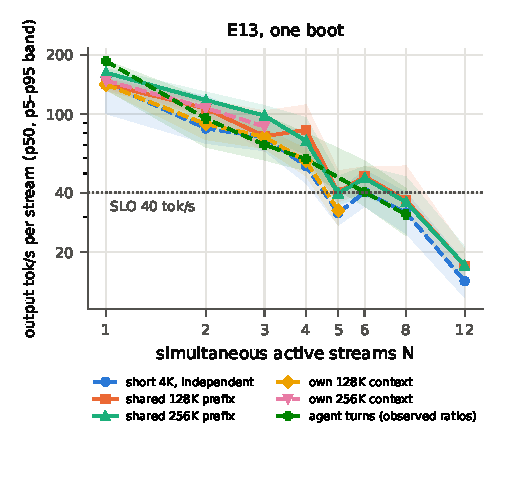
\includegraphics[width=0.49\linewidth]{figures/generated/agent_stream_rate.pdf}\hfill
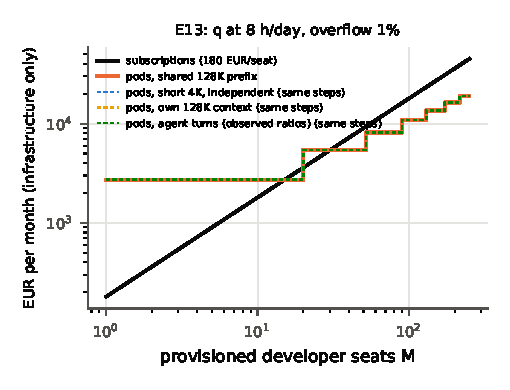
\includegraphics[width=0.49\linewidth]{figures/generated/agent_cost_seats.pdf}
\caption{Coding-agent case study, E13 (one boot). Left: median output rate per stream against simultaneous streams
(bands: p5 to p95 of requests), with the 40 tokens/s objective. Dashed lines are independent contexts. Right: monthly
cost of subscriptions and of the pods needed for $M$ provisioned seats, the larger of the volume and the concurrency
requirement (capacity with a 10\% margin, 50\% utilization, duty cycle for an 8-hour window, overflow probability 1\%),
infrastructure only. The four pod curves coincide because every regime has the same provisioning capacity.}
\label{fig:agent}
\end{figure}

% Generated by hostoffload.analysis.pipeline. Do not edit.
\begin{table}[t]
\centering
\small
\begin{fittable}{tab:agent-capacity}
\begin{tabular}{llrrrrrrrr}
\toprule
regime & source & C & C$_{+10\%}$ & p5 & p50 & p95 & TTFT p95 & aggr. & fails at \\
\midrule
short 4K, independent & E13 & 4 & 4 & 45 & 55 & 80 & 1.15 & 131 & 5 (32) \\
shared 128K prefix & E13 & 6 & 4 & 40 & 48 & 54 & 0.87 & 176 & 8 (37) \\
shared 256K prefix & E13 & 4 & 4 & 62 & 73 & 96 & 1.30 & 155 & 5 (40) \\
own 128K context & E13 & 4 & 4 & 49 & 58 & 67 & 1.72 & 172 & 5 (32) \\
own 256K context & E13 & $\ge$3 & $\ge$3 & 65 & 87 & 95 & 1.76 & 155 & - \\
agent turns (observed ratios) & E13 & 6 & 4 & 34 & 40 & 58 & 2.99 & 178 & 8 (31) \\
\bottomrule
\end{tabular}
\end{fittable}
\caption{Simultaneous streams at a median of at least 40 output tokens/s per stream. C is the largest N whose level and every smaller tested level meet it (failing on 2 or more errors above 5\%); per-stream rates (p5, p50, p95, tokens/s) and TTFT p95 (s) at C; the last column is the first failing N with its median rate. C$_{+10\%}$ is the same with a 10\% margin (44 tokens/s), used for provisioning.}
\label{tab:agent-capacity}
\end{table}

% Generated by hostoffload.analysis.pipeline. Do not edit.
\begin{table}[t]
\centering
\small
\begin{fittable}{tab:agent-levels}
\begin{tabular}{lrrrrrrrrrr}
\toprule
regime & N & rate p5 & p50 & p95 & TPOT p50 & p95 & TTFT p50 & p95 & err \% & aggr. \\
\midrule
short & 1 & 101 & 144 & 156 & 7.0 & 10.1 & 0.66 & 18.22 & 0 & 38 \\
short & 2 & 71 & 85 & 124 & 11.9 & 14.1 & 0.68 & 1.03 & 0 & 84 \\
short & 3 & 65 & 77 & 93 & 13.1 & 15.3 & 0.72 & 0.82 & 0 & 115 \\
short & 4 & 45 & 55 & 80 & 18.5 & 22.4 & 0.73 & 1.15 & 0 & 131 \\
short & 5 & 27 & 32 & 41 & 31.7 & 36.6 & 0.85 & 1.39 & 0 & 110 \\
short & 6 & 34 & 40 & 52 & 24.9 & 29.4 & 0.85 & 1.38 & 0 & 157 \\
short & 8 & 25 & 32 & 40 & 31.6 & 40.2 & 0.90 & 1.65 & 0 & 147 \\
short & 12 & 12 & 14 & 18 & 70.2 & 85.0 & 1.53 & 2.61 & 0 & 120 \\
cached128k & 1 & 132 & 142 & 152 & 7.0 & 7.6 & 0.61 & 0.63 & 0 & 118 \\
cached128k & 2 & 98 & 107 & 119 & 9.3 & 10.2 & 0.62 & 0.68 & 0 & 141 \\
cached128k & 3 & 69 & 77 & 104 & 12.9 & 14.6 & 0.72 & 0.80 & 0 & 145 \\
cached128k & 4 & 58 & 83 & 112 & 12.1 & 17.3 & 0.64 & 0.84 & 0 & 135 \\
cached128k & 5 & 36 & 40 & 52 & 25.0 & 27.8 & 0.74 & 0.88 & 0 & 155 \\
cached128k & 6 & 40 & 48 & 54 & 20.7 & 24.8 & 0.79 & 0.87 & 0 & 176 \\
cached128k & 8 & 32 & 37 & 55 & 27.3 & 31.8 & 0.84 & 1.00 & 0 & 178 \\
cached128k & 12 & 14 & 17 & 21 & 58.8 & 72.3 & 1.04 & 1.50 & 0 & 146 \\
cached256k & 1 & 146 & 162 & 171 & 6.2 & 6.8 & 0.96 & 1.02 & 0 & 113 \\
cached256k & 2 & 114 & 118 & 129 & 8.5 & 8.8 & 0.99 & 1.00 & 0 & 128 \\
cached256k & 3 & 77 & 98 & 111 & 10.2 & 13.1 & 1.02 & 1.17 & 0 & 155 \\
cached256k & 4 & 62 & 73 & 96 & 13.7 & 16.0 & 1.04 & 1.30 & 0 & 155 \\
cached256k & 5 & 35 & 40 & 48 & 25.2 & 28.8 & 1.08 & 1.53 & 0 & 131 \\
cached256k & 6 & 38 & 47 & 54 & 21.1 & 26.0 & 1.09 & 1.34 & 0 & 166 \\
cached256k & 8 & 32 & 36 & 48 & 27.9 & 31.7 & 1.34 & 1.67 & 0 & 212 \\
cached256k & 12 & 14 & 17 & 21 & 58.5 & 70.5 & 1.31 & 1.57 & 0 & 132 \\
own128k & 1 & 132 & 141 & 151 & 7.1 & 7.6 & 0.78 & 0.82 & 0 & 103 \\
own128k & 2 & 74 & 89 & 103 & 5.7 & 13.0 & 0.76 & 1.12 & 0 & 121 \\
own128k & 3 & 67 & 77 & 84 & 13.0 & 15.0 & 0.93 & 1.37 & 0 & 174 \\
own128k & 4 & 49 & 58 & 67 & 17.2 & 20.5 & 0.94 & 1.72 & 0 & 172 \\
own128k & 5 & 27 & 32 & 40 & 27.3 & 35.6 & 1.00 & 2.07 & 0 & 120 \\
own256k & 1 & 135 & 148 & 161 & 3.1 & 5.9 & 1.05 & 1.06 & 0 & 99 \\
own256k & 2 & 100 & 108 & 118 & 9.3 & 10.0 & 1.06 & 1.39 & 0 & 147 \\
own256k & 3 & 65 & 87 & 95 & 11.6 & 15.7 & 1.23 & 1.76 & 0 & 155 \\
agent & 1 & 134 & 186 & 188 & 5.4 & 7.6 & 0.91 & 0.94 & 0 & 133 \\
agent & 2 & 68 & 95 & 119 & 9.8 & 14.8 & 0.91 & 1.47 & 0 & 123 \\
agent & 3 & 59 & 70 & 98 & 14.3 & 17.2 & 0.97 & 2.08 & 0 & 146 \\
agent & 4 & 52 & 59 & 80 & 16.9 & 19.5 & 1.24 & 2.34 & 0 & 168 \\
agent & 6 & 34 & 40 & 58 & 24.9 & 29.3 & 1.37 & 2.99 & 0 & 178 \\
agent & 8 & 24 & 31 & 42 & 31.7 & 41.3 & 1.57 & 4.22 & 0 & 186 \\
\bottomrule
\end{tabular}
\end{fittable}
\caption{Controlled: E13 per level, part 1 of 2, service per stream. Per-stream rate p5/p50/p95 (tokens/s, tokens over end of stream minus first token), TPOT p50/p95 (ms), TTFT p50/p95 (s), failed requests (\%) and aggregate output (tokens/s). Resources at the same levels: Table~\ref{tab:agent-resources}.}
\label{tab:agent-levels}
\end{table}
\begin{table}[t]
\centering
\small
\begin{fittable}{tab:agent-resources}
\begin{tabular}{lrrrrrrrr}
\toprule
regime & N & GPU GiB & host GiB & PCIe GB/s & KV \% & hit \% & preempt. & bursts \\
\midrule
short & 1 & 86.2 & 214 & 15.09 & 3 & 0 & 0 & 0 \\
short & 2 & 86.3 & 214 & 38.12 & 4 & 0 & 0 & 0 \\
short & 3 & 86.4 & 214 & 55.41 & 4 & 0 & 0 & 0 \\
short & 4 & 87.6 & 214 & 57.15 & 7 & 0 & 0 & 0 \\
short & 5 & 87.6 & 214 & 80.81 & 5 & 0 & 0 & 0 \\
short & 6 & 87.6 & 214 & 72.06 & 8 & 0 & 0 & 0 \\
short & 8 & 87.6 & 214 & 75.27 & 9 & 0 & 0 & 0 \\
short & 12 & 89.9 & 214 & 91.26 & 17 & 0 & 0 & 0 \\
cached128k & 1 & 90.0 & 214 & 26.47 & 10 & 100 & 0 & 0 \\
cached128k & 2 & 90.0 & 214 & 36.93 & 10 & 100 & 0 & 0 \\
cached128k & 3 & 90.0 & 214 & 52.07 & 10 & 100 & 0 & 0 \\
cached128k & 4 & 90.0 & 214 & 57.82 & 10 & 100 & 0 & 0 \\
cached128k & 5 & 90.0 & 214 & 78.94 & 10 & 100 & 0 & 0 \\
cached128k & 6 & 90.6 & 214 & 71.71 & 11 & 100 & 0 & 0 \\
cached128k & 8 & 90.0 & 214 & 78.56 & 11 & 100 & 0 & 0 \\
cached128k & 12 & 90.0 & 214 & 90.66 & 12 & 100 & 0 & 0 \\
cached256k & 1 & 90.1 & 214 & 27.92 & 19 & 100 & 0 & 0 \\
cached256k & 2 & 90.1 & 214 & 42.66 & 19 & 100 & 0 & 0 \\
cached256k & 3 & 90.1 & 214 & 50.80 & 19 & 100 & 0 & 0 \\
cached256k & 4 & 90.1 & 214 & 55.81 & 19 & 100 & 0 & 0 \\
cached256k & 5 & 90.1 & 214 & 75.80 & 19 & 100 & 0 & 0 \\
cached256k & 6 & 90.1 & 214 & 72.85 & 20 & 100 & 0 & 0 \\
cached256k & 8 & 90.1 & 214 & 76.37 & 20 & 100 & 0 & 0 \\
cached256k & 12 & 90.1 & 214 & 88.75 & 21 & 100 & 0 & 0 \\
own128k & 1 & 90.1 & 214 & 50.15 & 10 & 100 & 0 & 0 \\
own128k & 2 & 90.1 & 214 & 70.71 & 19 & 100 & 0 & 2 \\
own128k & 3 & 90.1 & 214 & 65.54 & 29 & 100 & 0 & 0 \\
own128k & 4 & 90.1 & 214 & 72.83 & 39 & 100 & 0 & 1 \\
own128k & 5 & 90.1 & 214 & 84.21 & 48 & 100 & 0 & 1 \\
own256k & 1 & 90.1 & 214 & 49.08 & 19 & 100 & 0 & 1 \\
own256k & 2 & 90.1 & 214 & 55.53 & 38 & 100 & 0 & 0 \\
own256k & 3 & 90.1 & 214 & 59.58 & 56 & 100 & 0 & 0 \\
agent & 1 & 90.1 & 214 & 48.96 & 7 & 96 & 0 & 0 \\
agent & 2 & 90.1 & 214 & 65.56 & 17 & 96 & 0 & 1 \\
agent & 3 & 90.1 & 214 & 64.25 & 25 & 96 & 0 & 0 \\
agent & 4 & 90.1 & 214 & 75.86 & 34 & 96 & 0 & 0 \\
agent & 6 & 90.1 & 214 & 77.57 & 53 & 96 & 0 & 0 \\
agent & 8 & 90.1 & 214 & 81.58 & 62 & 96 & 0 & 0 \\
\bottomrule
\end{tabular}
\end{fittable}
\caption{Controlled: E13 per level, part 2 of 2, resources. Peak GPU memory per GPU (GiB), peak host anon+shmem (GiB), mean PCIe RX summed over GPUs (GB/s), peak KV-cache use (\%), prefix-cache hit rate (\%), preemptions, and requests whose reply arrived in one late burst (their TPOT is invalid; the per-stream rate of Table~\ref{tab:agent-levels} stays valid).}
\label{tab:agent-resources}
\end{table}


\paragraph{From stools to regulars.}
Developers do not keep the model writing all day. Of a whole week, the model was busy for this developer about
\dv{agent.dev.busy_h_week} hours, \dv{agent.q.week}\% of the week. We count each output token at 40 tokens/s and each
new context token at the reading rate E12 measured for a 128K-token prompt (\dv{agent.prefill_tok_s} tokens/s), which
makes this an upper bound, since faster service shortens it. Spread over an 8-hour working window on each active day,
the chance that the developer needs a stream at a random moment of that window is $q=\dv{agent.q.h8}\%$
(\dv{agent.q.h4}\% for a 4-hour window, \dv{agent.q.h24}\% for 24).

If $M$ developers work independently with the same $q$, the number who need a stream at once follows approximately a
Binomial$(M,q)$ distribution. A pod with $C$ stools can take the largest $M$ for which more than $C$ need one at once
only rarely. For agent turns ($C=\dv{agent.E13.agent.Cprov}$) that is \dv{agent.E13.agent.seats_conc_e1} developers if
the overflow may happen in fewer than one moment in a hundred, and \dv{agent.E13.agent.seats_conc_e5} at five in a
hundred (Tables~\ref{tab:agent-seats} and~\ref{tab:agent-duty}). An overflow does not fail requests. It means that the
streams of that moment fall below 40 tokens/s. The model ignores correlation between developers (shared working
hours, deadlines) and bursts within a session, both of which make overflows more frequent, so these numbers are
optimistic for a team on one schedule.

By volume the same pod looks much larger. At the total rate measured at four agent-turn streams, its monthly output
equals \dv{agent.E13.agent.seats_volume_u100} developers of this profile at full utilization and
\dv{agent.E13.agent.seats_volume_u50} at 50\%. The pod has the volume for \dv{agent.E13.agent.volume_over_conc_u50} to
\dv{agent.E13.agent.volume_over_conc_u100} times more intermittent developers than it can serve at 40 tokens/s at the
same moment, so the stools set the limit (Figure~\ref{fig:two-capacities}).

\begin{figure}[t]
\centering
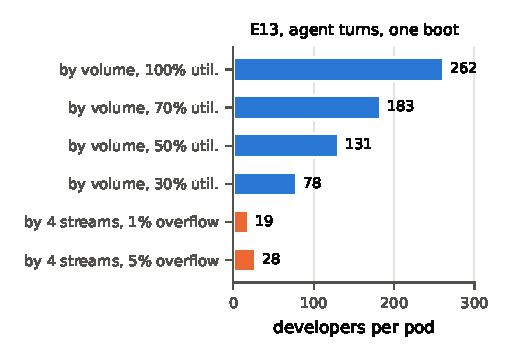
\includegraphics[width=0.62\linewidth]{figures/generated/agent_two_capacities.pdf}
\caption{The two capacities of one pod for agent turns (E13, one boot). Blue: developers whose monthly output the
pod can produce at the stated utilization. Orange: developers it can serve at 40 tokens/s or more each, with four
provisioned streams, an 8-hour active window and the stated probability that more than four want a stream at once.
Values from Table~\ref{tab:agent-seats}.}
\label{fig:two-capacities}
\end{figure}

To apply Table~\ref{tab:agent-duty} to another team, estimate how many hours a day its developers keep the agent
working, pick the row with that active window, and read the number of developers under the regime closest to how they
use context. A team that works in a narrower window concentrates its demand, so the same four stools take fewer
regulars.

% Generated by hostoffload.analysis.pipeline. Do not edit.
\begin{table}[t]
\centering
\small
\begin{fittable}{tab:agent-seats}
\begin{tabular}{lrrrrrrrrr}
\toprule
regime & C & aggr. & vol. 100\% & vol. 70\% & vol. 50\% & vol. 30\% & conc. 1\% & conc. 5\% & b.e. util. \% \\
\midrule
short 4K, independent & 4 & 131 & 204 & 143 & 102 & 61 & 19 & 28 & 7.4 \\
shared 128K prefix & 4 & 135 & 210 & 147 & 105 & 63 & 19 & 28 & 7.2 \\
shared 256K prefix & 4 & 155 & 242 & 169 & 121 & 73 & 19 & 28 & 6.3 \\
own 128K context & 4 & 172 & 268 & 188 & 134 & 81 & 19 & 28 & 5.6 \\
own 256K context & $\ge$3 & 155 & 242 & 170 & 121 & 73 & 12 & 20 & 6.2 \\
agent turns (observed ratios) & 4 & 168 & 262 & 183 & 131 & 78 & 19 & 28 & 5.8 \\
\bottomrule
\end{tabular}
\end{fittable}
\caption{Two capacities of one pod, provisioned on C with a 10\% margin (44 tokens/s). Volume: capacity-equivalent developer seats by observed monthly generation volume, at the aggregate output rate measured at that level and the stated utilization (these are NOT concurrent users). Concurrency: largest number of provisioned seats M with P(Binomial(M, q) > C) at most 1\% or 5\%, with q the duty cycle for an 8-hour active window. Last column: pod utilization at which the seats it serves would cost as much in subscriptions as the pod.}
\label{tab:agent-seats}
\end{table}

% Generated by hostoffload.analysis.pipeline. Do not edit.
\begin{table}[t]
\centering
\small
\begin{fittable}{tab:agent-duty}
\begin{tabular}{rrrrrrrr}
\toprule
active h/day & q \% & short & cached128k & cached256k & own128k & own256k & agent \\
\midrule
4 & 14.1 & 10 & 10 & 10 & 10 & 7 & 10 \\
8 & 7.1 & 19 & 19 & 19 & 19 & 12 & 19 \\
12 & 4.7 & 28 & 28 & 28 & 28 & 18 & 28 \\
24 & 2.4 & 55 & 55 & 55 & 55 & 36 & 55 \\
\bottomrule
\end{tabular}
\end{fittable}
\caption{Duty-cycle sensitivity. q is one developer's generating time (output at 40 tokens/s plus prefill of new tokens, from the usage sample) over an active window of the given hours on each of the 5 active days; cells are the largest M with P(Binomial(M, q) > C) at most 1\%.}
\label{tab:agent-duty}
\end{table}


\paragraph{What it costs against subscriptions.}
At \dv{agent.pod.eur_h}\,EUR an hour, a pod running all month costs \dv{agent.pod.eur_month}\,EUR, as much as
\dv{agent.break_even_seats} subscriptions of \dv{agent.seat_eur}\,EUR. One pod provisioned within its four stools
(\dv{agent.E13.agent.seats_conc_e1} developers) therefore lands just above break-even, and the next developer needs a
second pod, so 20 developers cost \dv{agent.E13.agent.cost.m20.extra}\,EUR a month more than subscriptions. Pooling
changes the picture, because the sum of many independent demands fluctuates less than each one. With load balanced
across pods, 100 developers need \dv{agent.E13.agent.cost.m100.pods} pods, \dv{agent.E13.agent.cost.m100.saving_pct}\%
below the cost of their subscriptions, and 250 need \dv{agent.E13.agent.cost.m250.pods},
\dv{agent.E13.agent.cost.m250.saving_pct}\% below, before engineering and operations (Table~\ref{tab:agent-cost},
Figure~\ref{fig:agent} right). Volume is never the constraint, since the pod breaks even at
\dv{agent.E13.agent.break_even_util}\% of its volume capacity. Stopping the pod outside a working window of
\dv{agent.pod.sched_hours} hours a month lowers its cost to \dv{agent.pod.sched_eur_month}\,EUR
(\dv{agent.break_even_seats_sched} subscriptions), but every start pays \dv{ctl.boot.min_minutes} to
\dv{ctl.boot.max_minutes} minutes of boot and weight loading and needs the \dv{static.pack.total_gib}\,GiB pack on
persistent storage. Engineering and operations move break-even substantially (Table~\ref{tab:agent-ops}), and those
amounts are assumptions, not measurements.

% Generated by hostoffload.analysis.pipeline. Do not edit.
\begin{table}[t]
\centering
\small
\begin{fittable}{tab:agent-cost}
\begin{tabular}{rrrrrrrrrr}
\toprule
seats & subs. EUR & pods cached128k & saving & pods short & saving & pods own128k & saving & pods agent & saving \\
\midrule
10 & 1,800 & 1 (c) & -923 & 1 (c) & -923 & 1 (c) & -923 & 1 (c) & -923 \\
15 & 2,700 & 1 (c) & -23 & 1 (c) & -23 & 1 (c) & -23 & 1 (c) & -23 \\
20 & 3,600 & 2 (c) & -1,847 & 2 (c) & -1,847 & 2 (c) & -1,847 & 2 (c) & -1,847 \\
25 & 4,500 & 2 (c) & -947 & 2 (c) & -947 & 2 (c) & -947 & 2 (c) & -947 \\
50 & 9,000 & 2 (c) & 3,553 & 2 (c) & 3,553 & 2 (c) & 3,553 & 2 (c) & 3,553 \\
100 & 18,000 & 4 (c) & 7,106 & 4 (c) & 7,106 & 4 (c) & 7,106 & 4 (c) & 7,106 \\
250 & 45,000 & 7 (c) & 25,936 & 7 (c) & 25,936 & 7 (c) & 25,936 & 7 (c) & 25,936 \\
\bottomrule
\end{tabular}
\end{fittable}
\caption{Subscriptions against self-hosted pods, infrastructure only (no engineering or operations). Pods per regime are the larger of the volume requirement (50\% utilization) and the concurrency requirement (P(demand > pods x C) at most 1\%, 8-hour window); v or c marks which binds. Savings are subscription cost minus pod cost per month, EUR; negative means self-hosting costs more.}
\label{tab:agent-cost}
\end{table}

% Generated by hostoffload.analysis.pipeline. Do not edit.
\begin{table}[t]
\centering
\small
\begin{fittable}{tab:agent-ops}
\begin{tabular}{rrrrr}
\toprule
ops EUR/month & 24/7 EUR & break-even & scheduled EUR & break-even \\
\midrule
0 & 2,723 & 15.1 & 985 & 5.5 \\
500 & 3,223 & 17.9 & 1,485 & 8.2 \\
1,500 & 4,223 & 23.5 & 2,485 & 13.8 \\
4,000 & 6,723 & 37.4 & 4,985 & 27.7 \\
\bottomrule
\end{tabular}
\end{fittable}
\caption{Operational overhead sensitivity for one pod: monthly cost and break-even subscription seats, 24/7 and scheduled (264 h/month). Overhead values are assumptions, not measurements.}
\label{tab:agent-ops}
\end{table}


\paragraph{Control of code and data.}
Price is not the only reason to run a coding agent's model in-house. With open weights the organization decides which
model and version run, when they change and how long prompts and outputs are kept. The source code, secrets and
internal documents that a coding agent reads by design (this profile re-reads \dv{agent.ratio.read_per_output} tokens
of context per token written) are not sent to a model provider, and the deployment can sit in a jurisdiction the
organization chooses, on its own hardware or with a provider bound by contract. These benefits of digital sovereignty,
privacy and data protection do not appear in the cost tables, and they come with two qualifications. They hold fully
only on hardware the organization controls. On a rented pod, as in our measurements, the data still reside on a third
party's machines, and their protection rests on that provider's isolation and contract. And self-hosting moves
responsibility rather than removing it, because security operations become the operator's work, part of the
operations overhead of Table~\ref{tab:agent-ops}. We measured no security property, so this paragraph describes what
the deployment model allows.

\paragraph{What the data support.}
Measured on one boot of one pod: four simultaneous coding-agent streams at 40 tokens/s or more each, whether the
context is short, a shared cached prefix of up to 256K tokens, an independent cached 128K-token context or agent turns
with the observed ratios, and a monthly volume for many times more developers of the observed profile. Derived under
stated assumptions (independent developers, an 8-hour window, 400-token replies): about
\dv{agent.E13.agent.seats_conc_e1} developers per pod at 1\% overflow, at the break-even of subscriptions for one pod
and below their cost for large pooled deployments. Not supported: any number transferred to another pod
(Section~\ref{sec:results-controlled} found a large difference between hosts), a real team's arrival pattern, or
replacing a commercial product. The workload, the usage profile and the cost model are specified in
Section~\ref{sec:method}, and the assumptions behind the seat counts are revisited in Section~\ref{sec:limits}.

\section{What It Means, and What Is Still Open}\label{sec:discussion}

\paragraph{What the offload makes possible.}
On two 96\,GB GPUs neither the original checkpoint nor the \dv{cfg.exl3_bits}-bit pack can keep all its experts in GPU
memory, and moving about a third of the experts to the host closes the last \dv{expl.noplan_over_per_gpu_gib}\,GiB per
card. The result serves a model whose unquantized version ranks first on agentic coding on LiveBench, on two GPUs that
can be rented by the hour. On the subsets we tested it matches the vendor's service within the uncertainty, and a long
context stays interactive once it is cached.

\paragraph{Practical guidance.}
For someone deploying this stack, four rules follow from the measurements. Each comes from a single boot on a specific
pod, so it is a starting point rather than a guarantee, and each names the check or the table to look at.
\begin{enumerate}
\item \emph{Check where the two GPUs sit before measuring or serving.} The same configuration had a median time per
token \dv{ctl.pod.cross.A.N1.tpot_ratio} to \dv{ctl.pod.cross.A.N32.tpot_ratio} times higher on a host where
\texttt{nvidia-smi topo -m} reports \texttt{\dv{ctl.pod.s2.gpu_link}} between the GPUs instead of
\texttt{\dv{ctl.pod.s1.gpu_link}} (and whose CPU also differed). Run \texttt{nvidia-smi topo -m} on the pod and
read the cell between GPU0 and GPU1. Our runners record it with the rest of the host (\datafile{experiments/lib.sh},
Tables~\ref{tab:pod-hardware} and~\ref{tab:cross-pod}).
\item \emph{Keep long contexts cached.} Once a 128K or 256K-token context is in the prefix cache, four streams keep a
median of \dv{agent.E13.own128k.prov.rate_p50} and \dv{agent.E13.cached256k.prov.rate_p50} tokens/s with TTFT p95
under two seconds, while a fresh 128K-token prompt costs \dv{ctl.E12.long.prefill-long-131072.closed:1.ttft_p50}\,s
of reading before its first token. Route the requests of one repository to the same server so that its prefix stays
in the cache (Figure~\ref{fig:read-write}, Tables~\ref{tab:ctl-E12} and~\ref{tab:agent-levels}).
\item \emph{Size interactive capacity in simultaneous streams, not tokens per month.} About
\dv{agent.E13.agent.Cprov} streams at 40 tokens/s per pod for agent turns, which under the observed usage profile
serve about \dv{agent.E13.agent.seats_conc_e1} intermittently active developers. Measure the team's active hours
and read the matching row of Table~\ref{tab:agent-duty}, and size the pods with Table~\ref{tab:agent-cost}.
\item \emph{Do not expect upstream vLLM's zero-copy offload to replace the recipe's hooks} on these pins. It does not
serve the model at all (Table~\ref{tab:ctl-E3}, with both KV block sizes).
\end{enumerate}

\paragraph{What we cannot yet explain.}
Each stream slows down as users are added, and we do not know which resource is responsible. The candidates are the
reads of cold experts over PCIe, the growing batch that speculative decoding must verify, interference from reading
new prompts, and the eager execution of decode steps larger than the biggest CUDA graph. Memory capacity is not among
them, since the pools are preallocated and did not move with load, and the KV cache was never the limit. The
experiments designed to separate the candidates (DSpark off, other placement policies, another SM budget for the
host-expert stream) did not run (Section~\ref{sec:not-run}). The same is true of placement. The plans are static and
derived from usage profiles, the recipe's own notes report that a plan tuned on one kind of traffic does worse on
another~\citep{diffbot2026dsv41exl3}, and recent systems argue that static placement is suboptimal in
general~\citep{he2026expertflow,zhong2025hybrimoe,zhu2026dali}. Our two nested plans show that a larger share on the
host costs throughput, and they say nothing about how much a better choice of experts would recover.
Section~\ref{sec:limits} lists every question the campaign leaves open, and Table~\ref{tab:plan} the experiments
written to answer them.

\section{Conclusion}\label{sec:conclusion}

A \dv{hub.orig.params_b}B-parameter model does not fit on two 96\,GB GPUs, even with its experts at
\dv{cfg.exl3_bits} bits, and a stack built by others makes it fit by moving its least-used experts to a back room in
host memory. The configuration boots and serves, matches the vendor's service within the uncertainty on the subsets we
tested, and for a single request keeps writing at nearly the same pace after reading a 256K-token prompt. It pays in
reading long prompts, in the speed of each stream as users are added, and in a sensitivity to the host as large as
most settings we varied. For coding agents, one server pours enough for a large team but has four stools, which
supports about \dv{agent.E13.agent.seats_conc_e1} developers who use the model now and then, close to the price of
their subscriptions, with larger pooled deployments below it. All of this rests on one boot per experiment.

The question in the introduction asked at what cost, and one part of the answer is still missing: how much speed the
offload costs against the same model held entirely in GPU memory. Measuring it needs larger GPUs and the original
checkpoint. The protocol is written, the variant is scripted to build from pinned sources, and the workload and the
analysis are the ones used throughout this paper. It has not yet been run, and on a prepared pod with two B300 GPUs
it is one command, \texttt{make bench-E9}.


\bigskip
\begin{center}\large\textbf{The Record}\end{center}
\noindent The rest of the paper holds what a reader needs to check or repeat the findings above: the earlier
exploratory runs that motivated the protocol, the full methodology with what each experiment actually ran, the setup
of the pods, related work, the limitations and threats to validity, and how every number is reproduced. It keeps the
level of detail of a methods section and can be read in any order.

\section{Exploratory Runs}\label{sec:results-exploratory}

This study began with runs made on 2026-10-06, before the protocol of Section~\ref{sec:method} existed. They are why
the protocol looks the way it does, and they are kept here for that reason, apart from the controlled results and
never mixed into their tables.

\noindent\fcolorbox{orange}{white}{\parbox{0.97\linewidth}{\small\textbf{\expl.} Everything in this section comes from
one run per configuration on a single pod, with all requests of a load level sent at once, usable bars chosen after
seeing the data, and no quality evaluation. The files are imported verbatim with hashes
(\datafile{data/exploratory/MANIFEST.tsv}), and the statistics below are recomputed from them by
\datafile{src/hostoffload/analysis/exploratory.py}.}}

\paragraph{What the first sweep showed.}
The sweep ran closed loops from $N=1$ to 64 users on the \texttt{\dv{expl.plan_identified.sweep}} plan
(Tables~\ref{tab:expl-sweep-A} and~\ref{tab:expl-sweep-B}, Figure~\ref{fig:expl-sweep}). With unique 4K-token code
prompts (scenario A), one request decoded at a median of \dv{expl.A.N1.decode_p50_tok_s} tokens/s and waited
\dv{expl.A.N1.ttft_p50_s}\,s for its first token. At eight users the median rate per request was
\dv{expl.A.N8.decode_p50_tok_s} tokens/s and at 64 it was \dv{expl.A.N64.decode_p50_tok_s}. The total output grew only
\dv{expl.A.agg_ratio_8_1}-fold from one user to eight and \dv{expl.A.agg_ratio_64_1}-fold to 64
(\dv{expl.A.N64.aggregate_out_tok_s} tokens/s). With a cached 16K-token prefix (scenario B) the total reached
\dv{expl.B.N64.aggregate_out_tok_s} tokens/s at 64 users and the median TTFT stayed at \dv{expl.B.N64.ttft_p50_s}\,s.
There were \dv{expl.A.errors_total} errors in \dv{expl.A.requests_total} requests in A and \dv{expl.B.errors_total} in
\dv{expl.B.requests_total} in B. This is the shape the controlled sweep later confirmed: concurrency buys total
throughput with each user's speed.

% Generated by hostoffload.analysis.pipeline. Do not edit.
\begin{table}[t]
\centering
\small
\begin{fittable}{tab:expl-sweep-A}
\begin{tabular}{rrrrrrrrrr}
\toprule
$N$ & $n$ & TTFT p50 & TTFT p95 & p95 later & decode p50 [CI] & p5 & aggr. & accept & USD/M out \\
\midrule
1 & 8 & 0.96 & 1.02 & 1.02 & 116.2 [113.0, 125.0] & 111.2 & 82.1 & 3.28 & 14.15 \\
2 & 8 & 0.99 & 1.80 & 1.80 & 70.9 [63.0, 94.7] & 54.0 & 112.2 & 3.39 & 10.35 \\
4 & 8 & 1.48 & 3.11 & 2.03 & 40.1 [33.8, 60.2] & 30.0 & 126.0 & 3.29 & 9.22 \\
8 & 16 & 2.04 & 4.99 & 2.55 & 23.1 [21.5, 26.3] & 16.7 & 152.1 & 3.37 & 7.63 \\
16 & 32 & 3.39 & 9.20 & 3.42 & 13.8 [13.3, 15.2] & 9.4 & 176.0 & 3.38 & 6.60 \\
32 & 64 & 5.05 & 18.47 & 5.82 & 8.2 [7.7, 9.1] & 5.8 & 209.3 & 3.37 & 5.55 \\
64 & 128 & 8.34 & 33.48 & 8.70 & 4.6 [4.3, 4.8] & 3.4 & 234.1 & 3.34 & 4.96 \\
\bottomrule
\end{tabular}
\end{fittable}
\par\smallskip\parbox{0.95\linewidth}{\footnotesize\raggedright Source: \texttt{data/exploratory/inferencekey-deepseek@546071a/vllm-exl3/pro6000-concurrency/results/scenario\_A.json}. ``p95 later'': TTFT p95 of requests sent after the first wave. Price: \texttt{experiments/pricing.yaml}.}
\caption{\textbf{EXPLORATORY} (single run, burst arrivals, not controlled). Scenario A: independent requests, a different 4K-token code prompt each (0 prefix-cache hits); 256 output tokens, closed loop, 2x RTX PRO 6000, DSpark $k=5$. TTFT and decode percentiles are nearest rank on $n$ requests (p95 is close to the maximum for $n<20$). Bracket: 95\% request-level bootstrap interval of the median, which ignores run-to-run variance. Cost: output-only attribution at the measured aggregate rate.}
\label{tab:expl-sweep-A}
\end{table}

% Generated by hostoffload.analysis.pipeline. Do not edit.
\begin{table}[t]
\centering
\small
\begin{fittable}{tab:expl-sweep-B}
\begin{tabular}{rrrrrrrrrr}
\toprule
$N$ & $n$ & TTFT p50 & TTFT p95 & p95 later & decode p50 [CI] & p5 & aggr. & accept & USD/M out \\
\midrule
1 & 8 & 0.41 & 0.49 & 0.42 & 136.4 [127.1, 149.6] & 121.8 & 113.0 & 3.87 & 10.28 \\
2 & 8 & 0.43 & 0.81 & 0.44 & 95.5 [84.5, 101.6] & 72.0 & 149.5 & 3.92 & 7.77 \\
4 & 8 & 0.49 & 0.94 & 0.79 & 61.7 [53.2, 72.4] & 51.2 & 208.2 & 3.90 & 5.58 \\
8 & 16 & 1.01 & 1.31 & 1.31 & 31.5 [29.7, 37.3] & 23.8 & 223.7 & 3.90 & 5.19 \\
16 & 32 & 1.44 & 1.81 & 1.81 & 18.8 [18.0, 20.8] & 15.0 & 264.8 & 3.95 & 4.38 \\
32 & 64 & 2.09 & 10.32 & 2.09 & 11.1 [10.7, 11.6] & 9.0 & 270.1 & 3.95 & 4.30 \\
64 & 128 & 2.23 & 4.39 & 2.45 & 7.1 [6.9, 7.3] & 6.0 & 398.2 & 4.03 & 2.92 \\
\bottomrule
\end{tabular}
\end{fittable}
\par\smallskip\parbox{0.95\linewidth}{\footnotesize\raggedright Source: \texttt{data/exploratory/inferencekey-deepseek@546071a/vllm-exl3/pro6000-concurrency/results/scenario\_B.json}. ``p95 later'': TTFT p95 of requests sent after the first wave. Price: \texttt{experiments/pricing.yaml}.}
\caption{\textbf{EXPLORATORY} (single run, burst arrivals, not controlled). Scenario B: 16K-token shared code prefix (cached) plus a short question; 256 output tokens, closed loop, 2x RTX PRO 6000, DSpark $k=5$. TTFT and decode percentiles are nearest rank on $n$ requests (p95 is close to the maximum for $n<20$). Bracket: 95\% request-level bootstrap interval of the median, which ignores run-to-run variance. Cost: output-only attribution at the measured aggregate rate.}
\label{tab:expl-sweep-B}
\end{table}


\paragraph{Three lessons that shaped the protocol.}
The first is about arrivals. Sending every request of a level at the same instant inflates the tail. In A at 64 users
the TTFT p95 was \dv{expl.A.N64.ttft_p95_s}\,s over all requests and \dv{expl.A.N64.ttft_p95_after_first_wave_s}\,s
over the requests sent after the first wave (Figure~\ref{fig:expl-ttft}), so the controlled protocol staggers starts,
which our runs did, and adds Poisson arrivals, which were designed but not run. The second is about content. DSpark
accepted on average \dv{expl.A.N8.spec_mean_accept_len} tokens per step in A and \dv{expl.B.N8.spec_mean_accept_len}
in B at eight users, and in the first run 480-token prose answers (an essay and two explanations) decoded at
\dv{expl.first.decode_480_0.decode_tok_s} to \dv{expl.first.decode_480_1.decode_tok_s} tokens/s for one stream,
against \dv{expl.A.N1.decode_p50_tok_s} for code reviews. Speed depends on what the model writes, which is why the
protocol separates code from prose and has an experiment with speculation off (E7, designed but not run, so every
controlled run used code prompts with DSpark on). The third is about attribution. These runs cannot say what the
offload costs: there is no run without it, because it does not fit, no run at another host share and no reference with
everything in GPU memory. The slowdown with more users may come from reads of host experts, from the growth of the
batch that speculation verifies, from interference by new prompts, or from decode steps larger than the biggest CUDA
graph running without one. The ablations designed to separate these (E4 to E7) did not run, so the controlled results
do not separate them either.

\begin{figure}[t]
\centering
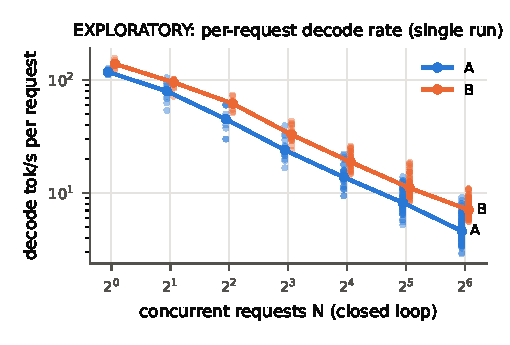
\includegraphics[width=0.49\linewidth]{figures/generated/exploratory_decode_per_request.pdf}\hfill
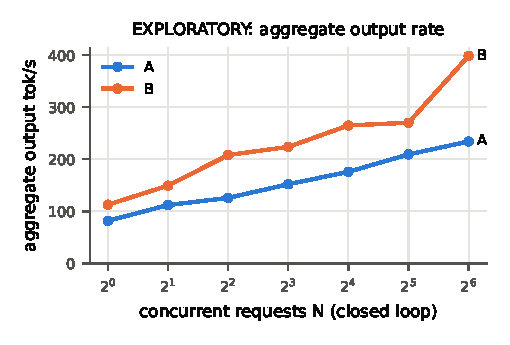
\includegraphics[width=0.49\linewidth]{figures/generated/exploratory_aggregate.pdf}
\caption{\expl{} (single run). Left: per-request decode rate (dots: requests, lines: medians) against concurrency.
Right: aggregate output rate. Sources: \texttt{scenario\_A.json} and \texttt{scenario\_B.json} in
\datafile{data/exploratory/inferencekey-deepseek@546071a/vllm-exl3/pro6000-concurrency/results/}.}
\label{fig:expl-sweep}
\end{figure}

\begin{figure}[t]
\centering
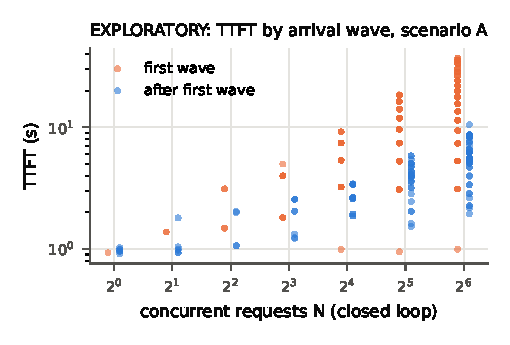
\includegraphics[width=0.49\linewidth]{figures/generated/exploratory_ttft_waves_A.pdf}\hfill
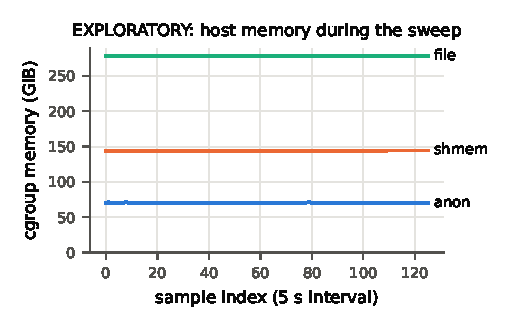
\includegraphics[width=0.49\linewidth]{figures/generated/exploratory_memory_timeline.pdf}
\caption{\expl{} (single run). Left: TTFT of first-wave requests (all sent at the start of a level) and of later
requests, scenario A. Right: host memory of the pod's cgroup during the sweep, 5\,s samples
(\texttt{mem\_samples.csv} in the folder of Figure~\ref{fig:expl-sweep}).}
\label{fig:expl-ttft}
\end{figure}

\paragraph{Memory stood still.}
The server reported \dv{expl.model_loading_gib}\,GiB of weights per GPU (loaded in \dv{expl.model_loading_s}\,s),
\dv{expl.cuda_graph_gib}\,GiB of CUDA graphs and a KV pool of \dv{expl.kv_tokens} tokens, enough for
\dv{expl.max_conc_x} requests at the full context limit. GPU memory stayed between \dv{expl.vram_min_peak_mib} and
\dv{expl.vram_peak_mib}\,MiB at every load level, because the pools are allocated in advance. Host memory did not move
with load either. Anonymous memory stayed between \dv{expl.ram_anon_min_gib} and \dv{expl.ram_anon_max_gib}\,GiB and
shared memory at \dv{expl.ram_shmem_gib}\,GiB, while the page cache filled the cgroup to
\dv{expl.ram_current_max_gib}\,GiB. The static split predicts \dv{static.gen30.host_gib}\,GiB of pinned file bytes for
this plan, more than the shared memory alone. These runs did not record how pinned buffers divide between anonymous
and shared mappings, and the controlled sampler dumps the largest mappings of every server process, but we have not
analyzed those dumps. Raising the context limit to 1M tokens raised the weight memory to
\dv{expl.1m.model_loading_gib}\,GiB and graphs to \dv{expl.1m.cuda_graph_gib}\,GiB per GPU and gave
\dv{expl.1m.kv_tokens} KV tokens from the same KV budget.

\paragraph{The first sign of prefix caching.}
In the first run a fresh code prompt of \dv{expl.first.ttft_16k.prompt_tokens} tokens took
\dv{expl.first.ttft_16k.ttft_s}\,s to its first token, and a second turn on the same prefix took
\dv{expl.first.ttft_16k_second_turn.ttft_s}\,s, with \dv{expl.first.ttft_16k_second_turn.cached} of
\dv{expl.first.ttft_16k_second_turn.prompt_tokens} prompt tokens served from the cache. That run's folder is named
\texttt{a100} after a sizing test, but it ran on the same 2x RTX PRO 6000 type
(\datafile{data/exploratory/inferencekey-deepseek@546071a/vllm-exl3/a100/results/agent30/bench.json}).

\paragraph{What the first sweep implied for cost.}
At the quoted pod price, with the whole hour charged to output tokens, the sweep implies
\dv{expl.A.N1.usd_per_m_out}\,USD per million output tokens for one user in A, \dv{expl.A.N8.usd_per_m_out} at eight
and \dv{expl.A.N64.usd_per_m_out} at 64, and \dv{expl.B.N1.usd_per_m_out}, \dv{expl.B.N8.usd_per_m_out} and
\dv{expl.B.N64.usd_per_m_out} in B. The cost per concurrent request falls as $1/N$, from \dv{expl.A.N1.usd_per_req_hour}
to \dv{expl.A.N64.usd_per_req_hour}\,USD per request-hour. Applying the pre-registered objectives (with TPOT p95
approximated by the inverse of the nearest-rank p5 decode rate, because that run did not store per-token times), the
interactive objective holds in A up to $N=\dv{expl.A.slo.interactive.N}$ at
\dv{expl.A.slo.interactive.usd_per_m_out}\,USD per million output tokens, the relaxed one up to
$N=\dv{expl.A.slo.relaxed.N}$ at \dv{expl.A.slo.relaxed.usd_per_m_out}\,USD, and the long-context one in B up to
$N=\dv{expl.B.slo.long_context.N}$ at \dv{expl.B.slo.long_context.usd_per_m_out}\,USD. With percentiles from 8 to 128
requests and burst arrivals, these numbers say where the frontier lies, not how precisely.

\section{PCIe Traffic and Speculative Decoding}\label{sec:bytes}

The samplers record each GPU's PCIe receive rate every half second (Table~\ref{tab:pcie-per-token}). Summed over both
GPUs it peaks at \dv{ctl.pcie.E8.B.N32.gbs}\,GB/s in E8 and \dv{ctl.pcie.E13.A.N12.gbs}\,GB/s in the coding-agent
experiment, against a line rate of \dv{ctl.pcie.calib.link_gbs}\,GB/s per GPU and direction for a PCIe Gen5 x16 link.
In E8 the bytes received per output token fall as users are added, from \dv{ctl.pcie.E8.A.N1.mb_per_tok} to
\dv{ctl.pcie.E8.A.N64.mb_per_tok}\,MB with unique prompts and from \dv{ctl.pcie.E8.B.N1.mb_per_tok} to
\dv{ctl.pcie.E8.B.N64.mb_per_tok}\,MB with the cached prefix, which is what one expects if one read of a host expert
serves several requests of a batch. In the coding-agent experiment they do not fall
(\dv{ctl.pcie.E13.A.N1.mb_per_tok}\,MB at one stream, \dv{ctl.pcie.E13.A.N12.mb_per_tok}\,MB at twelve in its short-session
regime), and we cannot explain the difference with these data. The two experiments differ in reply length (400 tokens
against 256), host (pod~3 against pod~1) and how far past saturation their sweeps went, and the counter mixes prompt
reading, drafter reads and expert reads, which we did not attribute. The counter itself is only partly validated. On
pod~1 a calibration script found NVML reporting \dv{ctl.pcie.calib.gpu0.copy.ratio} and
\dv{ctl.pcie.calib.gpu1.copy.ratio} times the true bytes for copies on GPU~0 and~1, and
\dv{ctl.pcie.calib.gpu0.zerocopy.ratio} times for zero-copy reads on GPU~0. The zero-copy test on GPU~1 is invalid, and
pods~2 and~3 have no calibration, so these values are raw and descriptive.

DSpark~\citep{cheng2026dspark,leviathan2023speculative}, the model's drafter, proposes \dv{ctl.spec.k} draft tokens per
step, and on code prompts a request gains on average \dv{ctl.spec.E8.A.accept_len} tokens per verification step with
unique prompts and \dv{ctl.spec.E8.B.accept_len} with the cached prefix (\dv{ctl.spec.E8.A.accept_rate_pct}\% and
\dv{ctl.spec.E8.B.accept_rate_pct}\% of proposed tokens accepted), almost independent of the number of users (in A
\dv{ctl.spec.E8.A.N1.accept_len} with one user and \dv{ctl.spec.E8.A.N64.accept_len} with 64,
Table~\ref{tab:spec-acceptance}). The coding-agent regimes, pooled over their levels, range from
\dv{ctl.spec.E13.A.accept_len} for short independent prompts to \dv{ctl.spec.E13.C256k.accept_len} for independent
256K-token contexts. All prompts were code or coding-agent turns with thinking off, so these values say nothing about
prose, and with speculation always on, its share of the speeds reported in the paper is not separated from the
offload's (E7, which would switch it off, did not run).

% Generated by hostoffload.analysis.pipeline. Do not edit.
\begin{table}[t]
\centering
\small
\begin{fittable}{tab:pcie-per-token}
\begin{tabular}{lrrr}
\toprule
regime & $N$ & PCIe RX GB/s & MB per output token \\
\midrule
E8 A: 4K independent & 1 & 25.2 & 473 \\
 & 8 & 72.4 & 395 \\
 & 64 & 66.3 & 231 \\
E8 B: 16K cached prefix & 1 & 36.5 & 326 \\
 & 8 & 76.2 & 356 \\
 & 64 & 68.2 & 150 \\
E13 short: 4K independent & 1 & 15.1 & 365 \\
 & 8 & 75.3 & 373 \\
 & 12 & 91.3 & 599 \\
E13 shared 128K prefix & 1 & 26.5 & 290 \\
 & 8 & 78.6 & 324 \\
 & 12 & 90.7 & 515 \\
E13 shared 256K prefix & 1 & 27.9 & 312 \\
 & 8 & 76.4 & 330 \\
 & 12 & 88.7 & 497 \\
E13 own 128K context & 1 & 50.2 & 455 \\
 & 5 & 84.2 & 570 \\
E13 own 256K context & 1 & 49.1 & 464 \\
 & 3 & 59.6 & 325 \\
E13 agent turns & 1 & 49.0 & 412 \\
 & 8 & 81.6 & 386 \\
\bottomrule
\end{tabular}
\end{fittable}
\par\smallskip\parbox{0.95\linewidth}{\footnotesize\raggedright Calibration on pod 1 (\texttt{data/controlled/E8-main/pcie-calibration.json}): NVML over true bytes 1.11 for DMA copies and 1.22 for zero-copy kernel reads on GPU 0. The GPU 1 zero-copy test is invalid: its nominal 294 GB/s exceeds the 63 GB/s PCIe 5.0 x16 line rate and NVML saw almost no traffic, so the kernel did not read over PCIe. Values are not corrected.}
\caption{PCIe receive traffic summed over both GPUs (NVML, raw counter) per level, and megabytes received per output token completed in the level window. E8 ran on pod 1 (two repetitions for B and for A at $N=1$, pooled), E13 on pod 3 (one repetition). Rows: $N=1$, $N=8$ and the largest tested $N$; every level is in \texttt{values.tex} (\texttt{ctl.pcie.*}). Descriptive: the bytes include prefill and drafter traffic.}
\label{tab:pcie-per-token}
\end{table}

% Generated by hostoffload.analysis.pipeline. Do not edit.
\begin{table}[t]
\centering
\small
\begin{fittable}{tab:spec-acceptance}
\begin{tabular}{lrrrrr}
\toprule
regime & $N$ & drafts & accepted/draft & accept. length & accepted \% \\
\midrule
E8 A: 4K independent & 1 & 1,139 & 2.39 & 3.39 & 48 \\
 & 8 & 1,192 & 2.44 & 3.44 & 49 \\
 & 64 & 9,744 & 2.37 & 3.37 & 47 \\
 & all & 20,627 & 2.37 & 3.37 & 47 \\
E8 B: 16K cached prefix & 1 & 1,134 & 2.63 & 3.63 & 53 \\
 & 8 & 2,318 & 2.54 & 3.54 & 51 \\
 & 64 & 18,279 & 2.58 & 3.58 & 52 \\
 & all & 37,575 & 2.60 & 3.60 & 52 \\
E13 short: 4K independent & 1 & 450 & 2.57 & 3.57 & 51 \\
 & 8 & 1,903 & 2.37 & 3.37 & 47 \\
 & 12 & 2,852 & 2.37 & 3.37 & 47 \\
 & all & 9,991 & 2.37 & 3.37 & 47 \\
E13 shared 128K prefix & 1 & 472 & 2.39 & 3.39 & 48 \\
 & 8 & 1,677 & 2.82 & 3.82 & 56 \\
 & 12 & 2,760 & 2.48 & 3.48 & 50 \\
 & all & 9,336 & 2.60 & 3.60 & 52 \\
E13 shared 256K prefix & 1 & 417 & 2.85 & 3.85 & 57 \\
 & 8 & 1,763 & 2.64 & 3.64 & 53 \\
 & 12 & 2,718 & 2.54 & 3.54 & 51 \\
 & all & 9,315 & 2.62 & 3.62 & 52 \\
E13 own 128K context & 1 & 223 & 2.60 & 3.60 & 52 \\
 & 5 & 1,063 & 2.77 & 3.77 & 55 \\
 & all & 3,272 & 2.67 & 3.67 & 53 \\
E13 own 256K context & 1 & 194 & 3.15 & 4.15 & 63 \\
 & 3 & 653 & 2.67 & 3.67 & 53 \\
 & all & 1,275 & 2.77 & 3.77 & 55 \\
E13 agent turns & 1 & 302 & 2.98 & 3.98 & 60 \\
 & 8 & 2,594 & 2.71 & 3.71 & 54 \\
 & all & 7,726 & 2.74 & 3.74 & 55 \\
\bottomrule
\end{tabular}
\end{fittable}
\caption{DSpark acceptance per level from vLLM's counters: drafts (\texttt{vllm:spec\_decode\_num\_drafts}), accepted draft tokens per draft, acceptance length $1 + \text{accepted}/\text{drafts}$ (tokens a request gains per verification step) and the share of proposed draft tokens accepted. Rows: $N=1$, $N=8$, the largest tested $N$ and all levels pooled; E8 on pod 1 (repetitions pooled), E13 on pod 3.}
\label{tab:spec-acceptance}
\end{table}


\section{Methodology}\label{sec:method}

The protocol was written to answer the paper's question in full, and our measurement campaign ran part of it. This
section gives both, the design and what actually ran, item by item, so that a reader can tell a measured result from a
designed one and can run the rest with the same tools.

\subsection{Six questions}
\begin{description}
\item[RQ1 (feasibility).] On two 96\,GB GPUs, which configurations of the model serve at all without host offload, and
with which exact failure do the others stop?
\item[RQ2 (cost of offload).] How do reading, writing, TTFT, TPOT and throughput change with the share of experts in
host memory, and how much of that is PCIe traffic?
\item[RQ3 (what the refinement adds).] At equal host bytes, how does Diffbot's per-expert split of hot and cold experts
compare with upstream vLLM's own selective zero-copy offload, and how much depends on the placement policy and its
match to the traffic?
\item[RQ4 (frontier).] What is the cost per token and per concurrent request under pre-registered service-level
objectives, from 1 to 64 users, and how does it compare with a reference that holds everything in GPU memory?
\item[RQ5 (quality).] How much accuracy does the \dv{cfg.exl3_bits}-bit stack lose against the original checkpoint on
reasoning, code, instruction following and long context?
\item[RQ6 (coding agents).] How many simultaneous coding-agent streams keep at least 40 output tokens/s each, and how
many intermittently active developers can share one pod under an observed usage profile (Section~\ref{sec:agent})?
\end{description}

\subsection{An ablation ladder}
To separate what each layer contributes, the protocol climbs a ladder in which each rung adds one layer on the same
hardware and with the same serving settings (\datafile{stack/variants/}, \datafile{experiments/experiments.yaml}).
\begin{enumerate}
\item[(a)] \textbf{upstream}: vLLM at the pinned commit, unpatched, with DeepSeek's original checkpoint. It is expected
to fail at load on two 96\,GB GPUs (Section~\ref{sec:system}), and E2 records the error. \textbf{upstream-uva} is the
same with upstream vLLM's selective zero-copy offload of the expert parameters, the closest upstream baseline that
may fit.
\item[(b)] \textbf{exl3-min} adds the five vLLM patches the pack needs on sm\_120, the unpatched vllm-exl3 plugin and
stock ExLlamaV3 kernels, with every expert in GPU memory. It is expected to fail at load, and E2 records it.
\item[(c0)] \textbf{exl3-uva} is (b) plus upstream vLLM's selective zero-copy offload of the EXL3 expert parameters,
sized to the same host bytes as a plan (\texttt{hostoffload.weights.plan bytes}).
\item[(c)] \textbf{exl3-offload} adds Diffbot's patch, kernels and hooks. Its factors are the plan (host shares from
25 to 60\%, chosen from routing counts of a calibration workload on a disjoint corpus half, the recipe's three plans,
and a seeded random plan with the same sizes per layer), the format of the Engram tables (int4, or FP8 if host memory
allows) and the number of SMs given to the host-expert stream.
\item[(d)] \textbf{DSpark on or off} on top of (c).
\end{enumerate}
A reference rung, \textbf{upstream on 2x B300}, serves the original checkpoint entirely in GPU memory (E9, E11). It is
the baseline of speed and quality that the offload has to be judged against, on different and more expensive
hardware.

\paragraph{The rungs that ran.} Our three pod sessions ran rung (b) and the offload build with an empty plan, both only
to the load failure (E2), rung (c0), which boots or fails but never serves (Section~\ref{sec:results-controlled}), and
rung (c) with DSpark on and two plans: the recipe's \texttt{gen30} plan and the union of its \texttt{gen30} and
\texttt{agent30} cold sets. Rung (a) and its upstream-uva variant (both with the original checkpoint), the calibrated,
random and FP8-Engram plans, the sweep of SM budgets, rung (d) and the B300 reference did not run
(Section~\ref{sec:not-run}).

\subsection{The benchmark protocol}
The harness (\datafile{src/hostoffload/harness/}) replaces the exploratory load generator and fixes the weaknesses
listed in Table~\ref{tab:fixes}. The protocol below is the full design (\datafile{experiments/workloads/main.yaml}),
and each item ends with what our runs used (\datafile{experiments/workloads/lean_main.yaml}, \datafile{experiments/workloads/lean_probes.yaml},
\datafile{experiments/workloads/lean_subset.yaml}, \datafile{experiments/workloads/long_context.yaml} and
\datafile{experiments/workloads/agent.yaml}, run by \datafile{experiments/runs/lean.sh},
\datafile{experiments/runs/long.sh} and \datafile{experiments/runs/agent.sh}).
\begin{itemize}
\item \textbf{Prompts} are cut to exact token counts with the server's own tokenizer endpoints, from pinned corpora:
the vLLM sources at the pinned commit for code, and four public-domain books for prose, both pinned by the sha256 of
the assembled text (\datafile{experiments/corpora.yaml}). Every prompt of a run is unique except deliberately shared
prefixes, and benchmark and calibration workloads use disjoint halves of the corpus. \emph{In our runs} it was as
designed, but every measured prompt came from the code corpus and the calibration workload did not run.
\item \textbf{Scenarios.} A sends independent 4K-token code prompts, A-Poisson the same as an open-loop Poisson stream
at five rates, B a 16K-token shared prefix (cached after one warm request) plus a question, P a 1K-token prose
continuation, where speculation is expected to accept fewer tokens, and L fresh 128K-token prompts. All use 256 output
tokens, temperature 0.6, top-p 0.95, a seed per request and thinking off. \emph{In our runs} only A and B ran in E8,
and neither A-Poisson nor P ran. Long prompts were measured by the separate experiment E12 (fresh prompts up to
260,000 tokens, decode after 128K and 256K-token prompts, and shared prefixes of 128K and 256K tokens), and E13 used
400-token replies (Section~\ref{sec:agent}).
\item \textbf{Arrivals.} Closed loops with $N\in\{1,2,4,8,16,32,64\}$ users whose starts are staggered over 10\,s, so
that there is no synchronized first wave, and Poisson open loops. A sweep stops when TTFT p95 exceeds 120\,s or more
than 5\% of requests fail, and the saturation point is recorded. \emph{In our runs} only closed loops ran. Starts were
staggered over 5\,s in the scenarios with independent short prompts or a shared prefix (E8, E3, the prefix scenarios
of E12 and regimes A and B of E13), but not in the decode scenarios after long prompts of E12 or in regimes C and D
of E13. In E8 and E3 scenario A each user sent two requests and each level had at least eight, and in the decode
probes one per user and at least four. The minimum of two errors in the error rule applies to E12 and E13 only (the
second session's rerun of E3 kept the first session's rule to match its baseline), and the long-context and agent
sweeps stop at a TTFT p95 of 900\,s.
\item \textbf{Reading and writing measured apart.} Prefill probes send unique prompts of 1K to 64K tokens with one
output token, one at a time, so that TTFT is reading plus an empty queue. Decode probes send 128-token prompts with
512 forced output tokens at each $N$, so that TPOT is writing under batching. Server-side histograms of queue, prefill
and decode time per request are differenced around every level. \emph{In our runs} the prefill probes used 4K, 16K and
64K tokens (three requests each), and the decode probes $N\in\{1,8,32\}$, with one repetition.
\item \textbf{Repetitions.} Three per load point within a boot, with fresh prompts and seeds each time, and three cold
boots at $N\in\{1,8,32\}$ for the component that varies between boots. Every request of every repetition is stored
raw. \emph{In our runs} there were no cold-boot repetitions, and each experiment's measurements come from a single
boot. The \texttt{gen30} configuration was booted on three pods, but no measurement was repeated across boots. E8 has
two repetitions per level in B and, after an early stop (Section~\ref{sec:results-controlled}), in A only at $N=1$.
E3, E12 and E13 have one. Every request is stored raw.
\end{itemize}

\begin{table}[t]
\centering\small
\begin{tabular}{p{4.1cm}p{5.6cm}p{4.5cm}}
\toprule
weakness of the exploratory runs & fix in the controlled protocol & in our runs \\
\midrule
single run per configuration & 3 repetitions per point plus 3 cold boots, cluster bootstrap over repetitions, variance components & partly: 1 or 2 repetitions inside one boot, no cold boots \\
usable bars chosen after seeing the data & SLOs registered in \datafile{experiments/sla.yaml} before any controlled run & yes \\
all $N$ requests sent at once (burst) & staggered closed-loop starts, plus open-loop Poisson arrivals & staggered starts (5\,s), no Poisson \\
speculation makes decode content-dependent & separate code and prose scenarios, DSpark on and off (E7), acceptance length recorded & partly: code only, DSpark always on, acceptance length recorded (Table~\ref{tab:spec-acceptance}) \\
quality never evaluated & E10 and E11 with lm-evaluation-harness against the original checkpoint & partly: three task subsets, DeepSeek's API as reference \\
per-chunk timing, several tokens per chunk & cumulative token counts on every chunk, per-token latency weighted by tokens & yes \\
corpus from the installed package, chars-per-token guess & pinned corpora, exact token counts via the server tokenizer & yes \\
5\,s sampler, no PCIe, no per-process memory & 0.5\,s sampler with NVML PCIe RX/TX, cgroup and per-process memory by kind, mapping dump & sampler yes, PCIe per level reported (Table~\ref{tab:pcie-per-token}), no Nsight capture, mappings not analyzed \\
plan of the sweep not recorded & plan path and sha256 in every run's configuration log & yes \\
aggregate rate includes ramp and drain & windowed aggregate rate (first send plus warm-up to last send) & yes \\
\bottomrule
\end{tabular}
\caption{Known weaknesses of the exploratory measurements, how the controlled protocol addresses them, and which fixes
our three pod sessions applied.}
\label{tab:fixes}
\end{table}

\subsection{What we compute}
TTFT is the arrival of the first streamed token minus the send time. TPOT is the time from the first to the last token
divided by the number of tokens after the first, and the per-request rate is its inverse. Per-token latency weights
each chunk's inter-arrival time by the tokens it carried. E2E is the end of the stream minus the send time. Aggregate
output throughput counts the tokens of requests that finished inside a window from the first send (plus a warm-up) to
the last send, so that ramp-up and drain do not dilute it. We report p50, p95 and p99 with linear interpolation, always
with $n$, and with fewer than 20 requests a p95 is close to the maximum. Requests of one repetition share server state,
so uncertainty comes from a bootstrap that resamples whole repetitions~\citep{efron1994bootstrap} and from the
coefficient of variation across repetitions, and a one-way variance decomposition separates the variance between and
within repetitions (\datafile{src/hostoffload/analysis/stats.py}).

\subsection{Following the bytes}
Zero-copy reads never show up as copies, so finding them takes several instruments. For every run we record the memory
of each GPU over time (NVML), the cgroup's anonymous, shared and file memory, each process's resident, anonymous,
shared, locked and pinned memory, the largest mappings of each server process at start, and the placement the server
logs at load (host experts per layer, Engram bytes per rank, weight, KV and graph memory). The static split
(Table~\ref{tab:static-placement}) gives file bytes per tensor class in GPU and host memory, and the runtime records
give allocations. PCIe receive and transmit rates per GPU come from NVML every 0.5\,s and from
\texttt{nvidia-smi dmon}, to be cross-checked by one Nsight Systems capture with GPU metrics and calibrated by a script
that drives a known volume of copy and zero-copy traffic and compares it with the counters
(\datafile{experiments/tools/pcie_calibrate.py}). The analysis correlates the PCIe receive rate with the decode rate
across load points and plans, with Pearson and Spearman coefficients and bootstrap intervals. \emph{In our runs} the
sampler and \texttt{nvidia-smi dmon} ran in every session and the calibration script once, in the first, where its
zero-copy test on the second GPU is invalid. We report PCIe receive traffic per level and per output token
(Section~\ref{sec:bytes}), but the Nsight capture, the attribution of allocations from the mappings and the
correlation analysis were not done.

\subsection{Cost and service-level objectives}
Cost per hour is the pod's quoted price in USD, converted to EUR at the ECB reference rate of \dv{price.fx.date}
(\dv{price.fx.usd_per_eur} USD per EUR, \datafile{experiments/pricing.yaml}). Cost per million output tokens divides
it by the sustained output rate. Splitting cost between input and output tokens is a modelling choice, so the model
offers three rules: all cost to output, a dedicated split (input cost from the prefill probe at saturation, output cost
from the decode probe), and a fixed price ratio solved at a mixed load point. Cost per concurrent request is the hourly
price divided by $N$, and cost per request is the level's pod time divided by its requests. Cost under an objective
uses the highest-throughput load point that meets it in every repetition. The three objectives are interactive (TTFT
p95 up to 2\,s and TPOT p95 up to 50\,ms), relaxed (10\,s and 100\,ms) and long context (5\,s and 66.7\,ms). They
were registered on 2026-10-06 before any controlled run, but after we had seen the exploratory data
(\datafile{experiments/sla.yaml}).

\subsection{Quality}
E10 and E11 run lm-evaluation-harness~\citep{sutawika2023lmeval} 0.4.13 (task names validated locally,
\datafile{quality/tasks.yaml}) against the measured stack and the reference. The design covers GSM8K~\citep{cobbe2021gsm8k}
and MATH-500~\citep{hendrycks2021math} for reasoning, HumanEval~\citep{chen2021humaneval} and MBPP~\citep{austin2021mbpp}
for code, IFEval~\citep{zhou2023ifeval} for instruction following, and subsets of RULER~\citep{hsieh2024ruler} and
LongBench~\citep{bai2024longbench} for long context. Both systems get identical prompts, greedy decoding, thinking off
and fixed seeds, with logs per item, so that differences are tested item by item with a paired bootstrap. Quantization
can change behaviour that averages hide~\citep{dutta2024accuracy}, so we also report the share of items whose outcome
flips. As designed, the reference is DeepSeek's original checkpoint on upstream vLLM on the B300 pod (E11). \emph{In
our runs} only fixed-seed subsets of GSM8K, IFEval and HumanEval were evaluated
(\datafile{quality/subsets_lean2h_seed20261006.json}), and the reference is the official DeepSeek API with thinking
disabled, reached through a local proxy that logs token usage (\datafile{quality/api_proxy.py}), reported separately
because its serving precision and implementation cannot be verified. MATH-500, MBPP, RULER and LongBench did not run.

\subsection{Designed but not run}\label{sec:not-run}
Six experiments of the protocol were designed and implemented but did not run in our campaign. Their full
specifications, workloads and runners are in \datafile{experiments/experiments.yaml} and \datafile{experiments/runs/},
and none of their numbers appears in this paper. E9 would serve the original checkpoint entirely in GPU memory on two
B300 GPUs, the reference against which the cost of the offload would be measured. E7 would turn DSpark off to separate
its effect, on code and on prose. E4 would compare placement policies at a fixed host share, including a random plan
and one fitted to our own routing counts. E5 would compare int4 and FP8 Engram tables in host memory. E6 would vary the
number of SMs given to the stream that computes host experts. E1 would rebuild every variant from scratch on a CPU
machine and record image digests.

\section{Experimental Setup}\label{sec:setup}

\paragraph{Hardware.}
Every controlled measurement ran on RunPod pods with two NVIDIA RTX PRO 6000 Blackwell Server Edition GPUs (sm\_120,
\dv{expl.gpu_total_mib}\,MiB reported per card), connected to the host over PCIe, at \dv{price.2xpro6000.usd_h}\,USD
per pod-hour (\dv{price.2xpro6000.eur_h}\,EUR). The exploratory pod had a cgroup memory limit of
\dv{expl.cgroup_max_gib}\,GiB. The designed reference (E9, not run) would use two B300 GPUs at
\dv{price.2xb300.usd_h}\,USD per hour, twice the single-GPU quote of \dv{price.1xb300.usd_h}\,USD. A single 80\,GB
A100 (\dv{price.1xa100.usd_h}\,USD per hour) is out of reach for two reasons: according to the exploratory notes the
pinned vLLM has no Ampere path for this model's sparse attention (Ampere support is an open feature request,
\datafile{audit/evidence/gh_issue_57144.json}), and neither checkpoint fits (Section~\ref{sec:system}). Every run
records the GPU model, driver, PCIe link generation and width, NUMA topology, CPU and cgroup limits
(\datafile{experiments/lib.sh}), and that record is what later explained part of the difference between hosts.

\paragraph{Software.}
All inputs are pinned in \datafile{stack/pins.env}: the vLLM nightly image by digest (vLLM \dv{expl.vllm_version}),
vllm-exl3 \texttt{d3cfd394}, ExLlamaV3 \texttt{5be88657}, the sfxnz recipe \texttt{460ac89c} and Diffbot's recipe at Hub
revision \texttt{a1cf1bd2}, verified file by file against \datafile{stack/recipe.lock.tsv}. Each variant is built
inside the pinned image by \datafile{stack/build/bootstrap_pod.sh} (or the Dockerfile wrapping it), which records
versions, git revisions, hashes of patched files and the full package list. Every variant shares the same serving
settings: tensor parallelism across the two GPUs, a context limit of 262,144 tokens, an fp8 KV cache of 4.25\,GiB, up to
64 sequences, 16,384 batched tokens per step, CUDA graphs for decode with capture sizes up to 256, prefix caching on,
and text only (\datafile{stack/serve.sh}).

\paragraph{Models.}
The EXL3 pack is \texttt{diffbot/DeepSeek-V4.1-Flash-EXL3-3bpw-2x-RTX-PRO-6000} at revision \texttt{a1cf1bd2}
(\dv{static.pack.total_gib}\,GiB), and the reference is \texttt{deepseek-ai/DeepSeek-V4.1-Flash} at \texttt{2cba9e42}
(\dv{static.orig.total_gib}\,GiB). Both are under the \dv{hub.orig.license} license as declared on the Hub
(\datafile{data/static/hub/}). Weights are downloaded on the pod at their pinned revisions and never redistributed.

\paragraph{Three sessions, three hosts.}
The campaign ran in three sessions on pods of this type, each on a different host. The first, on
\dv{lean.session.date}, lasted \dv{lean.session.minutes} minutes and ran E2, E8, E10 and E3. The second, on
\dv{lean.session2.date}, lasted \dv{lean.session2.minutes} minutes and ran E12, the E3 baseline again and the zero-copy
rung. The third lasted \dv{lean.session3.minutes} minutes and ran E13. Table~\ref{tab:pod-hardware} gives each host's
fingerprint. The GPUs, driver and PCIe link are the same, but the CPU model and the NUMA placement of the two GPUs are
not. The third session's record notes the first host's public IP, but its CPU and GPU bus ids differ, so it is a
different machine. The quality reference (E11) ran through DeepSeek's official API instead of on our own hardware.
Appendix~\ref{app:plan} lists the status of every experiment and how each session went.

% Generated by hostoffload.analysis.pipeline. Do not edit.
\begin{table}[!hb]
\centering
\small
\begin{fittable}{tab:pod-hardware}
\begin{tabular}{lp{2.4cm}p{2.2cm}rp{1.1cm}llp{1.2cm}p{1.6cm}}
\toprule
session & run & CPU & threads & GPU NUMA & GPU link & driver & PCIe max & bus ids \\
\midrule
1 (pod 1) & E8-main/main & AMD EPYC 9534 64-Core & 224 & 1, 1 & NODE & 595.91.07 & Gen5 x16 & 81:00.0, E1:00.0 \\
2 (pod 2) & E12-long-context/long & AMD EPYC 9535 64-Core & 256 & 0, 1 & SYS & 595.91.07 & Gen5 x16 & 06:00.0, 86:00.0 \\
3 (pod 3) & E13-coding-agent/agent & AMD EPYC 9535 64-Core & 256 & 1, 1 & NODE & 595.91.07 & Gen5 x16 & 86:00.0, F4:00.0 \\
\bottomrule
\end{tabular}
\end{fittable}
\caption{Hardware fingerprint of the three pod sessions (all 2x RTX PRO 6000 Blackwell Server Edition, same datacenter), from one run folder per session: CPU model and threads visible to the container (\texttt{fingerprint.json}), NUMA node of each GPU and the path between GPU0 and GPU1 (\texttt{nvidia-smi topo -m}: NODE within one NUMA node, SYS across the inter-socket link), driver, maximum PCIe link and GPU bus ids (\texttt{nvidia-smi -q}).}
\label{tab:pod-hardware}
\end{table}


\section{Related Work}\label{sec:related}

Every system that serves a model larger than its GPUs has to answer the same four questions: where the weights that
do not fit should live, whether the CPU should compute with them, how they reach the GPU when they are needed, and
whether the choice of what lives where is fixed or adapts at run time. This section uses those four questions to
place the stack we measured among the systems that came before it, after the serving machinery that all of them share.

\paragraph{Serving systems and batching.}
The evaluated stack runs on vLLM~\citep{kwon2023vllm,vllm2026github}, whose PagedAttention manages the KV cache in
fixed-size blocks, in the spirit of virtual memory paging, so that almost no memory is wasted and blocks can be shared
within and across requests. Orca~\citep{yu2022orca} introduced iteration-level scheduling, in which requests join and
leave the running batch between model iterations instead of between whole batches. Sarathi-Serve~\citep{agrawal2024sarathi}
splits long prompts into chunked prefills and schedules them without stalling ongoing decodes.
DistServe~\citep{zhong2024distserve} and Splitwise~\citep{patel2024splitwise} go further and place the prefill and
decode phases on different GPUs or machines, optimizing each for its own latency target (TTFT and TPOT, in DistServe's
terms). SGLang~\citep{zheng2024sglang} pairs a frontend language with a runtime that reuses the KV cache through
RadixAttention, and FlashInfer~\citep{ye2025flashinfer,flashinfer2026github} provides attention kernels with composable
block-sparse KV formats and a scheduler compatible with CUDA graphs. Host-resident experts add PCIe traffic on top of
this machinery.

\paragraph{Where idle experts can go.}
Sparse mixture-of-experts layers~\citep{shazeer2017outrageously,lepikhin2021gshard,fedus2022switch} activate a few
experts per token, so most expert weights are idle at any moment, which makes them natural candidates for slower
memory. DeepSpeed-MoE~\citep{rajbhandari2022deepspeedmoe} serves MoE models from aggregate GPU memory with expert
parallelism and does not offload. The systems that do offload fall into four families according to the four questions
above, and Table~\ref{tab:related-offload} places each one.

The first family keeps experts in host memory and \emph{copies} them into an expert cache on the GPU, hiding the
transfer with prediction. \citet{eliseev2023fast} keep an LRU cache of experts per layer and load experts speculatively
by applying the next layer's gate to the current hidden states, combined with mixed HQQ quantization.
MoE-Infinity~\citep{xue2024moeinfinity} traces expert activation per request and uses the trace to drive replacement
and prefetching. Pre-gated MoE~\citep{hwang2024pregated} changes the model itself, with a trained pre-gate that selects
the experts of the next block one block ahead so that only those are prefetched. SiDA~\citep{du2024sida} trains an
offline hash function that predicts expert activation and places experts on the GPU ahead of each batch.
ProMoE~\citep{song2024promoe} predicts later expert usage from intermediate results and fetches experts proactively,
AdapMoE~\citep{zhong2024adapmoe} adds sensitivity-based adaptive gating and a cache allocation per layer,
ExpertFlow~\citep{he2026expertflow} predicts routing paths for all layers with a learned predictor and schedules tokens
with similar routes together, and Fate~\citep{fang2025fate} uses a cross-layer gate for prefetching with a cache that
favors shallow layers and quantized cached experts. SwapMoE~\citep{kong2024swapmoe} and EdgeMoE~\citep{yi2025edgemoe}
target edge devices, the first by keeping a small dynamic set of important experts in memory and the second by
preloading predicted experts from storage with bit widths chosen per expert.

The second family aims at throughput and \emph{streams} weights layer by layer, spreading each transfer over a large
batch. FlexGen~\citep{sheng2023flexgen} and ZeRO-Inference, the heterogeneous component of
DeepSpeed-Inference~\citep{aminabadi2022deepspeedinference}, do this for dense models, FlexGen with a linear program
that splits weights, activations and KV cache across GPU, CPU and disk. MoE-Lightning~\citep{cao2025moelightning}
pipelines paged weight transfers with attention on the CPU under a performance model,
MoE-Gen~\citep{xu2025moegen} accumulates tokens in host memory to launch large batches per module on the GPU,
Klotski~\citep{fang2025klotski} overlaps expert loading with computation over several batches using a prefetcher aware
of expert correlations, and MoE-Lens~\citep{yuan2025moelens} derives its design from a holistic performance model of
CPU memory capacity and GPU compute.

The third family \emph{computes} cold experts on the CPU and moves activations instead of weights.
Fiddler~\citep{kamahori2025fiddler} places frequently used experts on the GPU from offline popularity profiling and,
for the remaining experts, chooses with a latency model between copying weights to the GPU and running the expert on
the CPU. KTransformers~\citep{chen2025ktransformers} keeps routed experts in CPU memory and runs them with CPU kernels
aware of arithmetic intensity and NUMA placement, keeps attention and shared experts on the GPU, and uses Expert
Deferral to overlap part of the expert work with the next layer's attention. HybriMoE~\citep{zhong2025hybrimoe},
DAOP~\citep{zhang2025daop} and DALI~\citep{zhu2026dali} schedule experts dynamically between CPU and GPU, and HybriMoE
and DALI argue explicitly that fixed assignments are inefficient because activation patterns vary.
eMoE~\citep{tairin2025emoe} combines learned expert prediction with request scheduling aware of service-level
objectives.

The fourth family, the one closest to the stack we measured, lets GPU kernels \emph{read host memory in place}.
DAK~\citep{lin2026dak} reads weights and KV cache directly from host memory without staging them in device memory,
with static offload ratios per operation from an offline sweep. Its abstract reports that direct access outperforms
prefetching, but it targets dense models. CUDA exposes the underlying mechanism as mapped, page-locked host memory in
a unified virtual address space~\citep{nvidia2026cudaguide}. In our search we found no peer-reviewed MoE system whose
GPU kernels execute host-resident expert weights in place. The only instance we found is the third-party software we
evaluate~\citep{vcruz2026vllmexl3,diffbot2026dsv41exl3}.

\begin{table}[t]
\centering
\small
\begin{fittable}{tab:related-offload}
\begin{tabular}{@{}l >{\raggedright\arraybackslash}p{1.55cm} >{\raggedright\arraybackslash}p{1.65cm} >{\raggedright\arraybackslash}p{3.0cm} >{\raggedright\arraybackslash}p{2.6cm} >{\raggedright\arraybackslash}p{1.95cm}@{}}
\toprule
System & Cold weights in & CPU computes & How weights reach the GPU & Placement & Quantization \\
\midrule
\multicolumn{6}{@{}l}{\emph{Copy into a GPU expert cache, hidden by prediction}} \\
\citet{eliseev2023fast} & host & no & copy, speculative prefetch & dynamic (LRU) & HQQ \\
MoE-Infinity~\citep{xue2024moeinfinity} & host & no & copy, prefetch & dynamic (activation-aware) & n.s. \\
Pre-gated MoE~\citep{hwang2024pregated} & host & no & copy, trained pre-gate & dynamic & n.s. \\
SiDA~\citep{du2024sida} & host & no & copy ahead of each batch & dynamic (offline-trained predictor) & no \\
ProMoE~\citep{song2024promoe} & host & no & copy, proactive prefetch & dynamic (LRU) & INT4 in evaluation \\
AdapMoE~\citep{zhong2024adapmoe} & host or SSD & no & copy, prefetch & dynamic (adaptive cache) & 4-bit \\
ExpertFlow~\citep{he2026expertflow} & host & no & copy, predictive & dynamic (predictive cache) & no \\
Fate~\citep{fang2025fate} & host & no & copy, prefetch & dynamic (ARC) & INT4, INT2 \\
\midrule
\multicolumn{6}{@{}l}{\emph{Stream weights, amortized over large batches}} \\
Klotski~\citep{fang2025klotski} & host, disk & no & copy, pipelined with batches & dynamic (correlation-aware) & 4-bit, optional \\
MoE-Lightning~\citep{cao2025moelightning} & host & attention only & copy, paged streaming & offline policy search & n.s. \\
MoE-Gen~\citep{xu2025moegen} & host & part of attention & copy, module batching & n.s. & n.s. \\
FlexGen$^\dagger$~\citep{sheng2023flexgen} & GPU, host, disk & optional attention & copy, layer streaming & offline LP & 4-bit \\
ZeRO-Inference$^\dagger$~\citep{aminabadi2022deepspeedinference} & host or NVMe & no & copy, layer prefetch & static & n.s. \\
\midrule
\multicolumn{6}{@{}l}{\emph{Compute cold experts on the CPU}} \\
Fiddler~\citep{kamahori2025fiddler} & host & yes & per expert: copy or CPU compute & static (offline profiling) & no \\
KTransformers~\citep{chen2025ktransformers} & host (routed experts) & yes & none: activations move & static & CPU block-wise \\
HybriMoE~\citep{zhong2025hybrimoe} & host & yes & copy or CPU compute & dynamic & 4-bit \\
DAOP~\citep{zhang2025daop} & host & yes & activations move to the CPU & calibrated, adjusted per sequence & n.s. \\
DALI~\citep{zhu2026dali} & host & yes & copy or CPU compute & dynamic & n.s. \\
\midrule
\multicolumn{6}{@{}l}{\emph{Read host memory in place from GPU kernels}} \\
DAK$^\dagger$~\citep{lin2026dak} & host & no & in place, direct kernel access & static (offline sweep) & n.s. \\
\textbf{Evaluated stack}~\citep{vcruz2026vllmexl3,diffbot2026dsv41exl3} & pinned host & no & in place, UVA zero-copy & static (usage profile) & EXL3, int4 Engram \\
\bottomrule
\end{tabular}
\end{fittable}
\caption{Qualitative positioning of offloading systems, grouped by how cold weights reach the computation and restricted
to facts stated in each paper (for the evaluated stack, in its documentation). ``Host'' is system memory (DRAM).
``Copy'' means host-resident weights are transferred into device memory before use, ``in place'' that GPU kernels read
host memory directly. $^\dagger$~dense model, all others are MoE. n.s.: not stated as part of the design in the text
we read.}
\label{tab:related-offload}
\end{table}

\paragraph{Making weights smaller.}
Post-training weight quantization ranges from scalar methods such as GPTQ~\citep{frantar2023gptq}, which uses
approximate second-order information, and AWQ~\citep{lin2024awq}, which protects salient channels identified from
activation statistics, to methods that also quantize activations, such as LLM.int8()~\citep{dettmers2022llmint8} with
its decomposition of outliers in mixed precision and SmoothQuant~\citep{xiao2023smoothquant}, which migrates the
difficulty of quantization from activations to weights. At three bits and below, incoherence processing and vector
codes dominate. QuIP~\citep{chee2023quip} introduced incoherence processing with random orthogonal transforms,
QuIP\#~\citep{tseng2024quipsharp} combined the randomized Hadamard transform with E$_8$ lattice codebooks, and
AQLM~\citep{egiazarian2024aqlm} adapted multi-codebook additive quantization. QTIP~\citep{tseng2024qtip} replaces
vector quantization with trellis-coded quantization, whose stateful decoder separates codebook size from bitrate and
effective dimension, and designs a bitshift trellis that is efficient in hardware. ExLlamaV3~\citep{turboderp2026exllamav3}
describes its EXL3 format as a streamlined variant of QTIP, and the evaluated plugin dispatches EXL3 routed experts
inside vLLM~\citep{vcruz2026vllmexl3}. For MoE models in particular, MoQE~\citep{kim2023moqe} reports that expert
layers are much more robust to quantization than dense feed-forward layers, QMoE~\citep{frantar2024qmoe} compresses
trillion-parameter MoE models below one bit per parameter with custom decoding kernels, MxMoE~\citep{duanmu2025mxmoe}
allocates mixed precision using both quantization sensitivity and expert activation frequency, MiLo~\citep{huang2025milo}
adds low-rank compensators to extremely quantized MoE models, and QuantMoE-Bench~\citep{li2024quantmoebench} studies
quantization heuristics aware of MoE structure. Quantization reduces the bytes that host-resident experts move over
PCIe, so it interacts directly with the offloading choices above.

\paragraph{Speculative decoding.}
Speculative decoding~\citep{leviathan2023speculative,chen2023accelerating} lets a cheap drafter propose tokens that the
target model verifies in parallel, preserving the target distribution, and blockwise parallel
decoding~\citep{stern2018blockwise} is an earlier form of draft and verify. Later work removes the separate draft model
or improves the drafts. Medusa~\citep{cai2024medusa} adds decoding heads verified with tree attention,
SpecInfer~\citep{miao2024specinfer} verifies token trees, and EAGLE~\citep{li2024eagle,li2024eagle2,li2025eagle3}
drafts at the feature level, with dynamic draft trees and, in EAGLE-3, direct token prediction with fusion of features
from several layers. \citet{gloeckle2024multitoken} train with multi-token prediction heads, and DeepSeek-V3 uses a
multi-token prediction objective in training~\citep{deepseekai2024v3}. Under batching the benefit is not automatic.
TurboSpec~\citep{liu2024turbospec} observes that naive speculation can degrade serving performance and adapts the
speculation length to predicted goodput, while MagicDec~\citep{sadhukhan2025magicdec} shows speedups at large batch
sizes for moderate to long sequences. \citet{xia2024unlocking} give a survey. DeepSeek-V4.1-Flash replaces the MTP
module with DSpark~\citep{deepseekai2026v41flash}, a semi-autoregressive drafter with confidence-scheduled
verification whose abstract reports per-user generation speedups of 60 to 85 percent at matched throughput over an
MTP-1 production baseline in DeepSeek's own serving system~\citep{cheng2026dspark}. In the evaluated stack part of the
drafter's experts are also host resident~\citep{diffbot2026dsv41exl3}, so drafting itself generates PCIe traffic.

\paragraph{Prefix caching and long context.}
Automatic prefix caching in vLLM~\citep{vllm2026prefixcaching} and RadixAttention in SGLang~\citep{zheng2024sglang}
reuse the KV cache of shared prefixes, which matters for multi-turn agentic sessions where most of each prompt repeats.
Chunked prefill~\citep{agrawal2024sarathi} bounds the latency impact of long prompts on concurrent decodes.
Long-context capability is commonly assessed with LongBench~\citep{bai2024longbench}, a bilingual multitask benchmark,
and RULER~\citep{hsieh2024ruler}, a synthetic benchmark with configurable length and task complexity.

\paragraph{The DeepSeek architecture.}
DeepSeekMoE~\citep{dai2024deepseekmoe} introduced fine-grained expert segmentation and shared expert isolation, and
DeepSeek-V3 added load balancing without an auxiliary loss~\citep{wang2024auxlossfree,deepseekai2024v3}.
DeepSeek-V2~\citep{deepseekai2024v2} introduced Multi-head Latent Attention (MLA), which compresses the KV cache into a
latent vector. Sparse attention followed with Native Sparse Attention~\citep{yuan2025nsa} and DeepSeek Sparse Attention
in DeepSeek-V3.2~\citep{deepseekai2025v32,deepseekai2025v32exp}, and DeepSeek-V4~\citep{deepseekai2026v4} combines
Compressed Sparse Attention with Heavily Compressed Attention for contexts of one million tokens.
DeepSeek-V4.1-Flash~\citep{deepseekai2026v41flash,deepseekai2026v41flashcard} has 552B backbone parameters, activates
16B parameters per token during decode and 8B during prefill, and reduces its global KV cache with cross-layer reuse in
Compressed Sparse Attention 2 and FP4 KV caching. Its model card lists 384 routed experts and one shared expert per MoE
layer, six routed experts active per token, and 196B parameters of Engram conditional memory accessed by token-based
lookup. Engram~\citep{cheng2026engram} (a conference version names the module Deep Sparse
Embedding~\citep{cheng2026dse}) modernizes $N$-gram embeddings for constant-time lookup and notes that deterministic
addressing allows prefetching from host memory, and the V4.1 report describes prefetching Engram embeddings from host
memory through background RDMA. The evaluated stack instead keeps int4 Engram tables in pinned host memory and reads
them over UVA inside CUDA graphs~\citep{diffbot2026dsv41exl3}.

\paragraph{Evaluating quantized and offloaded models.}
Common task suites for quality include GSM8K~\citep{cobbe2021gsm8k}, MATH~\citep{hendrycks2021math},
HumanEval~\citep{chen2021humaneval}, MBPP~\citep{austin2021mbpp}, LiveCodeBench~\citep{jain2025livecodebench} and
IFEval~\citep{zhou2023ifeval}, typically run through lm-evaluation-harness~\citep{sutawika2023lmeval}, whose
maintainers document the pitfalls of reproducing language-model evaluations~\citep{biderman2024lessons}. Matching
accuracy is not enough to show that a compressed model behaves like its reference. \citet{dutta2024accuracy} show that
answers flip between correct and incorrect even when aggregate accuracy is unchanged, and propose KL divergence and
flips as distance metrics. For DeepSeek-V4.1-Flash, AtomicChat published top-512 log-probability dumps and KL analyses
for an NVFP4 quantization~\citep{atomicchat2026dsv41metrics}, and the EXL3 checkpoints we use report KL against the
original model under that protocol~\citep{diffbot2026dsv41exl3,coolbho3k2026dsv41exl3}. On the performance side, MLPerf
Inference~\citep{reddi2020mlperf} prescribes rules for comparability across systems, \citet{agrawal2024etalon} argue
that TTFT and TPOT do not fully capture the latency users perceive, and the tools and statistics behind our
measurements are NVIDIA Nsight Systems and NVML~\citep{nvidia2026nsight,nvidia2026nvml} and the
bootstrap~\citep{efron1979bootstrap,efron1994bootstrap}.

\paragraph{Where the measured stack sits.}
The stack we evaluate is third-party software: the vllm-exl3 plugin by Victor Cruz (vcruz305)~\citep{vcruz2026vllmexl3},
which serves EXL3 routed experts in vLLM and offers an experimental mode in which packed expert weights are pinned in
host RAM while the GPU remains the compute device, and a host-expert patch with kernels by
Diffbot~\citep{diffbot2026dsv41exl3}, built on vLLM~\citep{kwon2023vllm} and ExLlamaV3~\citep{turboderp2026exllamav3}.
According to its documentation, the Diffbot configuration keeps a static set of cold experts in pinned host memory
(\dv{static.gen30.host_target_experts} of \dv{static.target_experts} routed experts in the plans it publishes, chosen
as those least used in long multi-turn agentic coding sessions), together with the int4 Engram tables and the
embedding table. GPU kernels read these weights in place over PCIe, the cold experts run on a second CUDA stream with a
bounded number of SMs while the experts in GPU memory run on the main stream, and there is neither computation of
experts on the CPU nor prefetching. Measured against the four questions, the design shares static, profile-derived
placement with Fiddler~\citep{kamahori2025fiddler} and KTransformers~\citep{chen2025ktransformers} but runs cold experts
on the GPU rather than the CPU. It shares direct kernel access to host memory with DAK~\citep{lin2026dak}, which
targets dense models, and with the zero-copy weight offload that upstream vLLM itself provides at the pinned commit,
which offloads whole parameter tensors (for a fused MoE layer, all of its experts) until a per-GPU budget is reached
(Section~\ref{sec:attribution}). And it differs from the cache and prefetch systems in that cold expert weights are read
in place rather than copied into a cache on the device. Several recent papers argue that static placement is
suboptimal~\citep{he2026expertflow,zhong2025hybrimoe,zhu2026dali}. Our controlled experiments measure one static
zero-copy placement on one hardware configuration at two host shares, without comparing against those systems on equal
terms and without testing other placement policies (Section~\ref{sec:not-run}). We claim no new algorithm or system.
Our contribution is a reproducible measurement of what this existing stack makes possible on two RTX PRO 6000
Blackwell GPUs, and at what cost in latency, throughput, memory, PCIe bandwidth and quality.

\section{Limitations and Threats to Validity}\label{sec:limits}

The findings of Sections~\ref{sec:background} to~\ref{sec:discussion} are only as strong as the measurements behind
them. This section says where they are weak, starting with the weakness that matters most.

\paragraph{One boot per experiment.}
The controlled evidence comes from three pod sessions on three different hosts (\dv{lean.session.minutes},
\dv{lean.session2.minutes} and \dv{lean.session3.minutes} minutes, Table~\ref{tab:pod-hardware}). Each experiment's
measurements come from a single boot. The \texttt{gen30} configuration was booted on all three pods, but no
measurement was repeated across boots, so the intervals cover repetitions inside a boot and nothing across boots. The
one configuration measured on two hosts differed by far more than any interval inside a boot
(Section~\ref{sec:results-controlled}), which makes the placement of a pod a large factor that we did not control. E8
has two repetitions per level in scenario B, but in scenario A only at $N=1$, because one client-side disconnect among
eight requests tripped the pre-registered stop rule (error rate above 5\%) and ended A's second sweep. A rule evaluated
on eight requests is too sensitive. After the first session we closed idle client connections before the server does,
which was the cause of those disconnects, and required at least two errors, a rule that E12 and E13 used. The second
session's rerun of the E3 subset kept the first session's rule to match its baseline, and the first session's data
were not rerun under the new rule.

\paragraph{The questions the campaign leaves open.}
Our three sessions (Section~\ref{sec:setup}) answer RQ1 on the measured hardware, give RQ2 two host shares with one
repetition each, measure the RQ4 frontier for two scenarios, give RQ5 a first answer on small subsets, and answer RQ6
for one pod and six context regimes with one repetition (E13, Section~\ref{sec:agent}). They leave open the following.
\begin{itemize}
\item The speed of the model held entirely in GPU memory, so that without the 2x B300 pod (E9) the cost of the offload
is bounded only by the slope between two host shares, not against a baseline without offload.
\item RQ3 as a comparison of speed, because without Diffbot's hooks the zero-copy variant cannot serve DeepSeek-V4.1 on
these pins at any KV block size (64 fails at initialization, 128 on the first request), so the cost of the per-expert
split against upstream's offload is unknown.
\item A quality reference on our own hardware and serving code, since the API stands in for E11 and differences may
come from the API's precision, prompt handling or sampling rather than from quantization.
\item Upstream vLLM with the original checkpoint on the same GPUs, dropped to avoid its \dv{static.orig.total_gib}\,GiB download.
\item Plans fitted to routing counts at several shares and the smallest share that fits, and the decode scenario at the
larger share, lost to a client-side disconnect.
\item Placement policy (E4), Engram format (E5), the SM budget of the host-expert stream (E6) and speculation off (E7).
\item The prose scenario, Poisson arrivals, MATH, MBPP, RULER and LongBench, while long context (E12) was measured with
one repetition, on the slower second pod, and without a quality check at those lengths.
\end{itemize}
Statements about these remain hypotheses.

\paragraph{Model capability.}
The LiveBench scores in Section~\ref{sec:background} belong to the unquantized model at maximum reasoning effort as
served by DeepSeek. How much of that capability survives \dv{cfg.exl3_bits}-bit quantization with thinking disabled is
not measured, since our quality evidence covers three small task subsets with thinking off. Running LiveBench on the
served stack, with thinking on and off, is future work.

\paragraph{The coding-agent case study.}
E13 is one repetition on one boot of one pod. Levels near the objective pass or fail by noise, which is why we
provision on a 10\% margin, and its capacities do not transfer to another pod (Section~\ref{sec:results-controlled}).
Replies have a fixed length of 400 tokens, and the agent turns are synthetic, with unique corpus text standing in for
tool output, so speculative decoding may accept more or fewer tokens than on real coding work. The usage profile is
one developer's week, read from a provider's billing categories that need not match vLLM's prefix-cache accounting, and
the reply length per turn and the daily active window are assumptions varied in the tables. The duty cycle uses the
floor of 40 tokens/s, an upper bound on busy time, and the Binomial model assumes independent developers with equal
activity, which understates the tail for a team on one schedule. Costs are GPU rental at one quoted price and exchange
rate. Storage, networking, engineering, operations and the differences in model capability and product features are
not priced, except in the stated sensitivity.

\paragraph{The exploratory data.}
The imported runs were measured once per configuration, used usable bars chosen after seeing the data, started every
level with a synchronized burst that dominates the TTFT tails, depend on content through speculative decoding with
synthetic prompts (slices of the vLLM sources and question templates, or a few essays), and never evaluated quality.
They also timed chunks rather than tokens, computed percentiles by nearest rank on 8 to 128 requests, measured
aggregate throughput including ramp-up and drain, and ran on one pod on one day.

\paragraph{The static accounting.}
File bytes are not runtime allocations. Repacking, FP8 copies and workspaces change the memory used on the GPU
(\dv{expl.runtime_minus_file_gib}\,GiB per GPU more in the exploratory boot). The placement rules model the documented
configuration and are checked against the server log only where the log reports placement. The minimal host share is
an estimate from one boot.

\paragraph{The protocol.}
The service-level objectives were registered before the controlled runs but after we saw the exploratory data. Cloud
pods share hosts, so CPU, memory bandwidth and PCIe topology vary between pods. We record them but cannot control
them, and repetitions across boots were designed for one pod and did not run. Upstream vLLM's zero-copy offload did
fail on this model at the pinned commit, at both KV block sizes we tried, and we report that failure as a result, but
it leaves RQ3 unanswered as a comparison of speed. When the B300 reference runs, it will bound the cost of the offload
together with the difference in hardware, because it uses other GPUs. GSM8K, HumanEval and similar benchmarks may be
in the training data, and since the comparison is between two versions of the same model, that limits the concern but
does not remove it. NVML's PCIe counters are sampled and their meaning varies between GPUs, hence the calibration
step.

\paragraph{Attribution.}
The audit relies on pinned public sources, keyword searches confirmed by reading code, and metadata from the Hub and
GitHub. Diffbot's code is attributed to the organization, because individual authors are not visible. Work that is
not public or not cited by the recipe could precede it.

\section{Reproducibility}\label{sec:repro}

A measurement study is only useful if someone else can repeat it. Everything in this paper comes out of the artifact
repository through documented commands.
\begin{itemize}
\item \texttt{make audit} reruns the attribution audit, with the sources fetched at their pins outside the repository.
\item \texttt{make static} measures the byte accounting and the Hub metadata again from public files.
\texttt{make test} runs the test suite, including the guard against numbers without data described below, and
\texttt{make analyze figures paper} regenerates every table, figure and value and builds this PDF.
\item \texttt{make stack-fetch} and \texttt{make pod-bootstrap VARIANT=\ldots} build each variant from pinned inputs
with recorded hashes. \texttt{make bench-E\textit{n}} and \texttt{make quality-E\textit{n}} run each experiment on a
prepared pod, and \texttt{make plan} regenerates the plan of experiments.
\end{itemize}

\paragraph{No number without a file.}
Every measured number in the text is printed by a macro that looks up a value written by the analysis pipeline. The
pipeline refuses values without an existing source file, refuses controlled values computed from exploratory files,
and records the sha256 of every source (\datafile{paper/generated/provenance.json}). Tables appear only for experiments
with data, so running one of the experiments of Section~\ref{sec:not-run} (\texttt{make bench-E\textit{n}}) adds its
table on the next build, and \texttt{STRICT=1} makes the build fail if any cited value lacks its source. A test fails
if a decimal number appears in the paper sources outside these macros, unless it is a whitelisted configuration
constant with its source (\datafile{paper/literal_numbers.yaml}).

\paragraph{From a finding to its data.}
Table~\ref{tab:trace} follows each row of Table~\ref{tab:key-results} back to the experiment, the script that ran it on
the pod, the folder that holds its raw data and the table or figure that prints it. The runners are the session
scripts of Appendix~\ref{app:plan}, and each folder has a README with the status of every run in it.

\begin{table}[h]
\centering\footnotesize
\begin{tabular}{>{\raggedright\arraybackslash}p{3.2cm}l>{\raggedright\arraybackslash}p{3.4cm}>{\raggedright\arraybackslash}p{3.6cm}>{\raggedright\arraybackslash}p{2.9cm}}
\toprule
finding & exp. & ran with & folder in \texttt{data/controlled/} & printed in \\
\midrule
fits only with the offload & E0, E2 & \texttt{make static}, \repolink{experiments/runs/lean.sh}{\texttt{lean.sh}} & \repolink{data/controlled/E2-feasibility/}{\texttt{E2-feasibility/}} (bytes: \datafile{data/static/weights/}) & Tables~\ref{tab:static-placement}, \ref{tab:ctl-E2} \\
reading against writing & E12, E3 & \repolink{experiments/runs/long.sh}{\texttt{long.sh}} & \repolink{data/controlled/E12-long-context/}{\texttt{E12-long-context/}} & Figure~\ref{fig:read-write}, Table~\ref{tab:ctl-E12} \\
one user and many & E8 & \repolink{experiments/runs/lean.sh}{\texttt{lean.sh}} & \repolink{data/controlled/E8-main/}{\texttt{E8-main/}} & Figure~\ref{fig:ctl-E8}, Table~\ref{tab:ctl-E8} \\
quality against the API & E10, E11 & \repolink{experiments/runs/lean.sh}{\texttt{lean.sh}}, \repolink{quality/api_proxy.py}{\texttt{api\_proxy.py}} & \repolink{data/controlled/E10-quality-exl3/}{\texttt{E10-quality-exl3/}}, \repolink{data/controlled/E11-quality-reference/}{\texttt{E11-quality-reference/}} & Table~\ref{tab:ctl-quality-paired} \\
streams and developers & E13 & \repolink{experiments/runs/agent.sh}{\texttt{agent.sh}} & \repolink{data/controlled/E13-coding-agent/}{\texttt{E13-coding-agent/}} & Figures~\ref{fig:agent}, \ref{fig:two-capacities}, Tables~\ref{tab:agent-capacity}, \ref{tab:agent-seats} \\
upstream offload alone & E3 & \repolink{experiments/runs/lean.sh}{\texttt{lean.sh}}, \repolink{experiments/runs/long.sh}{\texttt{long.sh}} & \repolink{data/controlled/E3-host-share/}{\texttt{E3-host-share/}} & Table~\ref{tab:ctl-E3} \\
the host matters & E3 & \repolink{experiments/runs/lean.sh}{\texttt{lean.sh}}, \repolink{experiments/runs/long.sh}{\texttt{long.sh}} & \repolink{data/controlled/E3-host-share/}{\texttt{E3-host-share/}}, \repolink{data/controlled/LEAN/}{\texttt{LEAN/}} & Tables~\ref{tab:cross-pod}, \ref{tab:pod-hardware} \\
\bottomrule
\end{tabular}
\caption{Traceability of the findings in Table~\ref{tab:key-results}. Session runners are in
\datafile{experiments/runs/}, the API proxy in \datafile{quality/}.}
\label{tab:trace}
\end{table}

\paragraph{Licenses and redistribution.}
The repository contains no third-party source code. The recipe, the plugin and the kernels are fetched and patched at
build time from pinned revisions. vllm-exl3 and Diffbot's patch to it are AGPL-3.0, so a built image that includes
them carries AGPL obligations when distributed or served with modifications. Our code is Apache-2.0, compatible with
vLLM's license and combinable with the AGPL components in a built image, and text and data are CC-BY-4.0. Model weights
are never redistributed (\datafile{THIRD_PARTY.md}, \datafile{PROVENANCE.md}).

\paragraph{Archival.}
The repository is prepared for an archived release with a persistent identifier (\datafile{CITATION.cff},
\datafile{.zenodo.json}, \datafile{RELEASE_CHECKLIST.md}).

\paragraph{Availability.}
The artifact repository, \url{https://github.com/inferencekey/vllm-exl3-moe-hostoffload}, holds the code, the
stack configurations, the workloads, the raw data and the sources of this paper, and every file named in the text
links to it. The configurations that
make the model boot (the variant builds, the expert plans and the session runners) are the ones measured here and
can be reused to serve the model on the same class of hardware.


\section*{Acknowledgments}
This paper measures open work by others. We thank Victor Cruz, whose vllm-exl3 plugin brings EXL3 to vLLM and is the
base on which the host-memory offload is built; turboderp for ExLlamaV3 and the EXL3 format; Diffbot for the serving
recipe, the host-expert patch and its kernels; coolbho3k for the 3-bit EXL3 checkpoint; sfxnz for the recipe helpers;
Mia's AI Lab for the work vllm-exl3 derives from; the vLLM project and the authors of the pull requests the recipe
carries; and DeepSeek for releasing the model's weights. None of them took part in this study, and any error is ours.

\bibliographystyle{plainnat}
\bibliography{references}

\appendix
\section{Experiment Plan and Status}\label{app:plan}

Table~\ref{tab:plan} lists every experiment of the protocol (\datafile{experiments/experiments.yaml}), whether it ran,
and where its data are. Hours and commands of the full and minimal plans are in \datafile{experiments/PLAN.md}. The
experiments that did not run keep their workloads, runners and data folders in the repository, and running one makes
its table appear in the paper on the next build.

\paragraph{The campaign.}
The campaign that ran is a reduced version of the protocol, called the \emph{lean plan} in the repository
(\datafile{experiments/runs/lean.sh}). Its first session runs on one 2x RTX PRO 6000 pod of at most
\dv{lean.hard_cap_minutes} minutes, paying boot, build and the weight download once. It covers the setup, E2 reduced to
the two EXL3 boots without offload, E8 with scenarios A and B at all seven concurrency levels, two repetitions and the
probes, E10 on fixed-seed subsets of GSM8K, IFEval and HumanEval, and E3 reduced to the \texttt{gen30} plan against
upstream's zero-copy offload at the \texttt{gen30} host bytes, with one repetition at $N\in\{1,8,32\}$. A final
optional step adds a larger nested plan, the union of the \texttt{gen30} and \texttt{agent30} cold sets. The runner
checks the remaining time before every step, so that a session ends cleanly instead of in the middle of a
measurement.

\paragraph{How each session went.}
The first session ran on \dv{lean.session.date} for \dv{lean.session.minutes} minutes
(\datafile{data/controlled/LEAN/session.json}). It completed every step, including the optional one, plus a repeat of
E10 after the continuation fix of Section~\ref{sec:quality}. Two bootstrap bugs forced two restarts before the first
valid boot: git refused the copied sources, and a patch check could not tell whether overlapping patches had been
applied. Both are fixed in \datafile{stack/build/bootstrap_pod.sh}. The second session, on \dv{lean.session2.date}
(\dv{lean.session2.minutes} minutes, \datafile{experiments/runs/long.sh}), ran on a different host. A first attempt
was aborted by a third bootstrap bug, a git configuration step that ran before git was installed, and its boots were
invalid and stayed on the pod. The session then ran the long-context experiment E12, the E3 \texttt{gen30} point again
as a baseline on the same pod, and the zero-copy rung with the KV block size it needs. The third session
(\dv{lean.session3.minutes} minutes, \datafile{experiments/runs/agent.sh}) ran on a third host, whose record notes the
first host's public IP but a different CPU model and GPU bus ids (Table~\ref{tab:pod-hardware}). It ran the
coding-agent experiment E13 after a first attempt that stopped before any measurement because the image lacked git.

\paragraph{The quality reference.}
The quality reference is the official DeepSeek API, whose \texttt{deepseek-flash} model is served by
DeepSeek-V4.1-Flash according to its pricing page (fetched 2026-10-06, \datafile{data/static/pricing/}). The run sent
\dv{ctl.E11.api.requests} requests, all answered, through the proxy that logs the real token counts.

\begin{table}[h]
\centering\small
\begin{tabular}{llp{6.2cm}p{3.6cm}}
\toprule
id & GPUs & question & status \\
\midrule
E0 & none & static byte accounting & done (Section~\ref{sec:system}) \\
E1 & CPU & reproducible build of every variant, image digests and provenance & not run \\
E2 & 2x PRO 6000 & feasibility without host offload, exact failure & ran (session 1, EXL3 rungs only) \\
E3 & 2x PRO 6000 & host share, upstream zero-copy offload at equal host bytes & ran (two shares, sessions 1 and 2, zero-copy cannot serve) \\
E4 & 2x PRO 6000 & placement policy at 30\%: recipe plans, random, our profile plan & not run \\
E5 & 2x PRO 6000 & Engram int4 vs FP8 in host memory & not run \\
E6 & 2x PRO 6000 & SM budget of the host-expert stream & not run \\
E7 & 2x PRO 6000 & DSpark on vs off, code vs prose & not run \\
E8 & 2x PRO 6000 & main benchmark: $N$ = 1 to 64, probes, memory, PCIe & ran (session 1, closed loop, two repetitions in B, one in A beyond $N=1$ and in the probes) \\
E9 & 2x B300 & upstream reference with everything in GPU memory, original checkpoint & not run \\
E10 & 2x PRO 6000 & quality of the EXL3 stack & ran (session 1, fixed subsets) \\
E11 & 2x B300 & quality of the reference & ran through DeepSeek's API instead \\
E12 & 2x PRO 6000 & long context at 128K and 256K tokens & ran (session 2) \\
E13 & 2x PRO 6000 & coding-agent workload, streams at 40 tokens/s & ran (session 3) \\
\bottomrule
\end{tabular}
\caption{Controlled experiments and their status. Sessions: \datafile{data/controlled/LEAN/session.json},
\datafile{data/controlled/LEAN/session2.json}, \datafile{data/controlled/LEAN/session3.json}.}
\label{tab:plan}
\end{table}


\end{document}
